\documentclass[12pt]{article}

\usepackage{notes}

\def\showsolutions{}

\begin{document}
 
\title{EECS 445 Lecture Notes}
\author{Matthew Jia}
\maketitle

\part{Lecture 1}

Supervised Learning: Training data has a fatures \textbf{and} labels (i.e. the training data has the answer/classification for each example)\\
Binary Classification Problem: A machine learning problem where you are given features of a data point and you want to classify the data point into two possible groups (ex: a review is helpful or not helpful)

If each problem has a discrete finite set of possible labels, we call these problems a Classification Problem. If there are only two possible labels, then it is a Binary Classification Problem. Linear classifiers are when you split the space of possible features into two parts using a hyperplane.

\newpage

\part{Lecture 2}

\section{Supervised Learning}
A model that is trained on features \textbf{with} labels

\subsection{Classification as an ML problem}
Each datapoint has the following:

\begin{enumerate}[label=\arabic*.]
	\item 
		Features are statistics or attributes that describe the data

		Feature vector for datapoint i is denoted as
		\[ \bar{x}^{(i)} \in \R^d \]
		Where $d$ is the dimensionality of the feature
	\item 
		The label for datapoint $i$ is denotes as
		\[ y^{(i)} = \{ -1, +1 \} \]
		For binary classifiers
\end{enumerate}

The training dataset is the set of datapoints used to train the model. It takes the form:

\[ S_n = \{ \bar{x}^{(i)}, y^{(i)} \}_{i=1}^n \]

Our goal, given the training dataset, is to learn the \underline{linear} decision boundary. Afterwards, we can use this boundary to predict future test points.

\subsection{Why a linear decision boundary?}

Our goal is to find a general solution to a problem, not overfit to the training data. Thus, a linear boundary is better than a arbitrary shape that fits perfectly to a dataset because it can generalize the solution/model.

\section{Linear Classifiers}

Start off with the following assumptions:

\begin{enumerate}
	\item only choose hyperplanes that go through the origin
	\item Constrain problem to datasets that are linearly seperable
\end{enumerate}

\subsection{Hyperplanes}

\subsection{Definition}

A hyperplane in $\R^d$ can be specified by parameter vector $\bar{\theta} \in \R^d$ and offset $b \in \R$. It is the set of points $\bar{x} \in \R^d$ such that 
\[ \bar{\theta} \cdot \bar{x} + b = 0 \]

Note that $\bar{\theta}$ is orthogonal to the hyperplane $\bar{\theta} \cdot \bar{x} = 0$

\subsection{Linear Classification in 2D}

Claim: For any vector $\bar{x}' \in \R^d$, if $\bar{x}'$ lies on the same side of the hyperplane $\bar{\theta} \cdot \bar{x} = 0$ as $\bar{\theta}$, $\bar{\theta} \cdot \bar{x}' > 0$. The converse if true.

\begin{proof}~\\
	\[ \bar{\theta} \cdot \bar{x} = ||\bar{\theta}||_2 ||\bar{x}||_2 \cos \alpha\]
	
	Where $\alpha$ is the angle between $\bar{\theta}$ and $\bar{x}$. $\cos \alpha$ is positive in the 1st and 4th quatrant, meaning the dot product is positive in the range $(-\frac {\pi} 2, \frac {\pi} 2)$. This happens to be the same side of the hyperplane as $\bar{\theta}$.
\end{proof}

Using this previous claim, we will define our linear classifier (that goes through the origin) as 

\[ h(\bar{x};\bar{\theta}) = sign(\bar{\theta} \cdot \bar{x}) \]

Points that lie on the hyperplanes are assumed to be misclassified.\\

The choice of $\bar{\theta}$ determines:
\begin{enumerate}
	\item orientation of the hyperplane
	\item the predicted class label
\end{enumerate}

\subsection{Linear Separability: Definition}

Given training examples 
\[ S_n = \{ \bar{x}^{(i)}, y^{(i)} \}_{i=1}^n \]
we say the data are \emph{linearly separable} if there exists $\bar{\theta} \in \R^d$ such that

\begin{center}
	$sign(\bar{\theta} \cdot \bar{x}^{(i)})$ agrees with $y^{(i)}$
\end{center}

Observe that if $sign(\bar{\theta} \cdot \bar{x}^{(i)})$ agrees with $y^{(i)}$, then $y^{(i)}(\bar{\theta} \cdot \bar{x}^{(i)}) > 0$\\

\textbf{Note:} This is the definition for datasets that are linearly separable using hyperplanes that go through the origin. 

\subsection{Selecting $\bar{\theta}$}

\begin{itemize}
	\item Find $\bar{\theta}$ that works well on training data $S_n = \{ \bar{x}^{(i)}, y^{(i)} \}_{i=1}^n$
	\item The training error is defined as
		\[ E_n(\bar{\theta}) = \frac 1 n \sum_{i=1}^n [[y^{(i)}(\bar{\theta} \cdot \bar{x}) \le 0 ]] \]
		Where $[[p]]$ is an indicator function that follows
		\[ 
			[[p]] = \begin{cases}
				1, & p \text{ is true}\\
				0, & \text{otherwise}\\
			\end{cases}
		\]
\end{itemize}

\subsection{Perceptron Algorithm}

This is an algorithm to find $\bar{\theta}$.\\

\begin{algorithm} \label{alg:perceptron}
\caption{Perceptron Algorithm}
\begin{algorithmic}
\State $k \gets 0$, $\bar{\theta}^{(0)} \gets \bar{0}$
\While{there exists a misclassified point}
    \For{$i = 1, \dots, n$}
        \If{$y^{(i)}(\bar{\theta}^{(k)} \cdot \bar{x}^{(i)}) \le 0$}
            \State $\bar{\theta}^{(k+1)} \gets \bar{\theta}^{(k)} + y^{(i)}\bar{x}^{(i)}$
						\State $k \gets k + 1$
        \EndIf
    \EndFor
\EndWhile
\end{algorithmic}
\end{algorithm}

In words, it initializes $\bar{\theta}$ and loops until a $\bar{\theta}$ creates a separating hyperplane. Inside the loop, it checks for all points that are misclassified by the current hyperplane defined by $\bar{\theta}$ and tilts the $\bar{\theta}$ towards those points. \\

\textbf{Note:} This algorithm does not halt on some inputs, i.e., the inputs that are not linearly separable.

\newpage

\part{Lecture 3}

\section{The Perceptron Update}

Let us focus on the steps that update the hyperplane in the Perceptron Algorithm (\ref{alg:perceptron}). First, observe that the update only happens if $y^{(i)}(\bar{\theta}^{(k)} \cdot \bar{x}^{(i)}) \le 0$. This only happens when the signs of $y^{(i)}$ and $\bar{\theta}^{(k)} \cdot \bar{x}^{(i)}$ are different, i.e., the label differs with the way the hyperplane is oriented with respect to point (i). This makes sense, since you only really want to update the oritentation of the hyperplane if it disagrees with a point.\\

Secondly, notice what the update does. It sets $\bar{\theta}^{(k+1)} = \bar{\theta}^{(k)} + y^{(i)}\bar{x}^{(i)}$. Its not super obvious how this change to the hyperplane is effective directly from an analysis on $\bar{\theta}^{(k+1)}$. Instead, we will see what this does to the next prediction of point (i):

\[ 
	\begin{aligned}
		y^{(i)}(\bar{\theta}^{(k+1)} \cdot \bar{x}^{(i)}) &= y^{(i)}((\bar{\theta}^{(k)} + y^{(i)}x^{(i)}) \cdot \bar{x}^{(i)})\\
																											&= y^{(i)}(\bar{\theta}^{(k)} \cdot x^{(i)}) + (y^{(i)})^2||\bar{x}^{(i)}||_2^2\\
																											&= y^{(i)}(\bar{\theta}^{(k)} \cdot \bar{x}^{(i)}) + ||\bar{x}^{(i)}||_2^2
	\end{aligned}
\]

Overall, the updated guess will be nudged towards being positive. Thus, you are causing the hyperplane to make a ``better" guess with respect to the current data point.

\subsection{Important Observations}

\begin{itemize}
	\item The perceptron algo updates based on a single (missclassified) point at a time. Not sure why this is useful yet.
	\item The algo moves the hyperplane in the `right' direction based on that point.
\end{itemize}

\subsection{Quiz 1}

Given the following data points, find the value of $\bar{\theta}$ after the first iteration of the Perceptron algo.\\

\begin{tabular}{lccc}
\toprule
      & Dimension 1 & Dimension 2 & Label \\
\midrule
Datapoint 1 & 6 & 6 & + \\
Datapoint 2 & 9 & 1 & - \\
\bottomrule
\end{tabular}~\\

\begin{solution}~\\
	1st datapoint: $\bar{\theta}^{(0)}$ will be updated since $\bar{\theta}^{(0)} = \bar{0}$, and $\bar{0} \cdot \bar{x} = 0 \le 0$ for all $\bar{x}$. We get
	\[
		\bar{\theta}^{(1)} = 
		\begin{bmatrix}
			0\\
			0
		\end{bmatrix} +
		\begin{bmatrix}
			6\\
			6
		\end{bmatrix} = 
		\begin{bmatrix}
			6\\
			6
		\end{bmatrix}
	\]\\

	2nd datapoint: $\bar{\theta}^{(1)}$ will be updated since $y^{(1)}(\bar{\theta}^{(1)} \cdot \bar{x}^{(1)}) = -1(6 \cdot 9 + 6 \cdot 1) = -60 \le 0$. We get
	\[
		\bar{\theta}^{(2)} = 
		\begin{bmatrix}
			6\\
			6
		\end{bmatrix} + 
		(-1)\begin{bmatrix}
			9\\
			1
		\end{bmatrix} = 
		\begin{bmatrix}
			-3\\
			5
		\end{bmatrix}
	\]\\

\end{solution}

\textbf{Note:} It is possible for the perceptron algo to missclassify the first datapoint after processing the second datapoint, since it could overcompensate and move the hyperplane too far. It is also possible for the algo to missclassify the second datapoint even after processing it, since it could undercompensate and move the hyperplane too little.

\section{Perceptron with Offset}

\subsection{Linearly Separable with Offset: Definition}

Given training examples 
\[ S_n = \{ (\bar{x}^{(i)}, y^{(i)}), \}_{i=1}^n \]
we say the data are \emph{linearly separable} if there exists $b \in \R$ and $\bar{\theta} \in \R^d$ such that

\begin{center}
	$y^{(i)}(\bar{\theta} \cdot \bar{x}^{(i)} + b) > 0$
\end{center}

for $i = 1, \dots, n$.\\
We refer to 
\[ \bar{x}: \bar{\theta} \cdot \bar{x} + b = 0 \]
as a separating hyperplane

\subsection{Perceptron Algorithm (Modified)}

\textbf{Goal:} Learn $\bar{\theta}$ that minimizes training error

\[ E_n(\bar{\theta}) = \frac 1 n \sum_{i=1}^n [[y^{(i)}(\bar{\theta} \cdot \bar{x} + b) \le 0 ]] \]

Since we added a new dimension (offset) to the problem, we will be adding an extra dimension to our feature vector $\bar{x}^{(i)} \in \R^d$. This extra dimension will be the first index of our column vector and will be set to 1 for all feature vectors, giving us\\

\[ 
	\bar{x}^{(i)'} = 
	\begin{bmatrix}
		1\\
		x_1^{(i)}\\
		\dots\\
		x_d^{(i)}
	\end{bmatrix}
\]

Observe (for the Perceptron Algorithm Algorithm) that, at convergence, 

\[
	\begin{aligned}
								& \forall i, y^{(i)}(\bar{\theta}^{(k)'}) \cdot \bar{x}^{(t)'} > 0\\
		\rightarrow & \forall i, y^{(i)}
		\left(
			\begin{bmatrix}
				\theta_0^{(k)}\\
				\theta_1^{(k)}\\
				\dots\\
				\theta_d^{(k)}\\
			\end{bmatrix}
		\right)
		\cdot
			\begin{bmatrix}
				1\\
				x_1^{(k)}\\
				\dots\\
				x_d^{(k)}\\
			\end{bmatrix}
		> 0\\
		\rightarrow & \forall i, y^{(i)}(\bar{\theta}^{(k)} \cdot \bar{x}^{(t)} + \theta_0^{(k)}) > 0\\
	\end{aligned}
\] 

Amazingly, with the extremely small change of adding an extra dimension to our feature vectors, our perceptron algo works exactly as before without modification, and will find the hyperplane to a linearly separable dataset even if it must contain an offset. 

\section{Loss functions and Gradient Descent}

What if our dataset is not linearly separable?\\

\textbf{Idea:} focus on minimizing empirical risk\\
\textbf{Goal:} Find parameter vector $\bar{\theta}$ that minimizes the empirical risk:

\[ R_n(\bar{\theta}) = \frac 1 n \sum_{i=1}^n Loss(h(\bar{x}^{(i)};\bar{\theta}), y^{(i)}) = \frac 1 n \sum_{i=1}^n Loss(y^{(i)}(\bar{\theta} \cdot \bar{x}^{(i)})) \]

Example of loss functions for linear classifiers:

\begin{itemize}
	\item 0-1 Loss function
		\[ R_n(\bar{\theta}) = \frac 1 n \sum_{i=1}^n [[y^{(i)}(\bar{\theta} \cdot \bar{x}^{(i)}) \le 0]] \]
	\item Hinge loss function
\end{itemize}

\subsection{Hinge loss function}

\textbf{Idea:} minimize empirical risk using gradient descent

\[ R_n(\bar{\theta}) = \frac 1 n \sum_{i=1}^n max((1 - y^{(i)}(\bar{\theta} \cdot \bar{x}^{(i)})), 0) \]

Hinge loss functions are nice because they incorporate the idea of ``worse" mistakes (if $y^{(i)}(\bar{\theta} \cdot \bar{x}^{(i)})$ is more negative, then the function incurs more loss. We can visualize this with a datapoint that is very far from the hyperplane and on the wrong side), and it also forces predictions to be more than just a ``little correct" (this is done by adding the 1 in the term $1 - y^{(i)}(\bar{\theta} \cdot \bar{x}^{(i)})$, guesses that are barely correct will have a lower $y^{(i)}(\bar{\theta} \cdot \bar{x}^{(i)})$ value and thus would still incur loss from this loss function).\\

The hinge loss function is a convex function, which are characterized by bowl shapes when plotted on a graph. 

\subsection{Gradient Descent (GD)}

\textbf{Goal:} Find the value of parameter $\bar{\theta}$ that minimizes training error $R_n(\bar{\theta})$\\
Initial guess on minimizer $\bar{\theta} = \bar{0}$ and for some (variable or fixed) step size $\eta$\\

Update guess on $\bar{\theta}$:

\[ \bar{\theta}^{(k+1)} = \bar{\theta}^{(k)} - \eta \nabla_{\bar{\theta}}R_n(\bar{\theta}) |_{\bar{\theta} = \bar{\theta}^k}  \]


\part{Lecture 4}

From last lecture, we started looking at Datasets that are not linearly separable. The perceptron algorithm does not work perfectly on these datasets due to its halting condition, which is defined as the moment when all datapoints are correctly classified. Another problem with perceptron is that it doesn't get the line of least loss; it only gets $\bar{\theta}$ that separates the dataset. Thus, we began to look at a new algorithm, called gradient descent, that tries to solve these two problems.

\subsection{Convergence Criteria}

We have a couple of options for this:

\begin{enumerate}
	\item Keep track of $R_n(\bar{\theta})$ (halt the algorithm if our Loss function doesn't seem to classify our data well?? (check if this is right))
	\item Keep track of $\bar{\theta}$ (bound the algorithm by rate of change of $\bar{\theta}$)
	\item Keep track of $k$ (bound the algorithm by number of interations)
\end{enumerate}

\subsection{Step Size}

We don't want $\eta$ to be too big because it might give us an inaccurate $\bar{\theta}$. We also don't want $\eta$ to be too small because the algorithm might take too long. We also don't want step size to be too large because corrections to $\bar{\theta}$ might overshoot the optimzal value for the dataset and result in more error.\\

Often we set $\eta_k = 1/(k+1)$

Our classic GD algorithm looks like this:

\begin{algorithm} \label{alg:GD}
	\caption{Linear Classification Using Gradient Descent}
	\begin{algorithmic}
		\State $k \gets 0$, $\bar{\theta}^{(0)} \gets \bar{0}$
		\While{convergence criteria is not met}
		\State $\bar{\theta}^{(k+1)} \gets \bar{\theta}^{(k)} - \frac{\eta_k} {n} \sum_{i = 1}^n \nabla_{\bar{\theta}} Loss(y^{(i)}(\bar{\theta} \cdot \bar x^{(i)}))$
		\State $k \gets k + 1$
		\EndWhile
	\end{algorithmic}
\end{algorithm}

\subsection{Issues with GD}

Remember that 

\[ \bar{\theta}^{(k+1)} = \bar{\theta}^{(k)} - \eta \nabla_{\bar{\theta}}R_n(\bar{\theta}) |_{\bar{\theta} = \bar{\theta}^k}  \]

and 

\[ R_n(\bar{\theta}) = \frac 1 n \sum_{i=1}^n max((1 - y^{(i)}(\bar{\theta} \cdot \bar{x}^{(i)})), 0) \]

To find $\nabla R_n(\bar{\theta})$, we need to find the partial derivative of each point. This happens on \textbf{each} update of $\bar{\theta}$, which is incredibly slow!!

\section{Stochastic Gradient Descent (SGD)}

\textbf{Idea:} Instead of looping over all examples before update, update based on a single point. We use a combination of perceptron and GD here.

\[ R_n(\bar{\theta}) = \frac 1 n \sum_{i=1}^n max((1 - y^{(i)}(\bar{\theta} \cdot \bar{x}^{(i)})), 0) \]

\begin{algorithm}
	\caption{Linear Classification Using Stochastic Gradient Descent}
	\begin{algorithmic}
		\State $k \gets 0$, $\bar{\theta}^{(0)} \gets \bar{0}$
		\While{convergence criteria is not met}
		\State randomly shuffle points
		\For{$i = 1, \dots, n$}
		\State $\bar{\theta}^{(k+1)} \gets \bar{\theta}^{(k)} - \eta_k \nabla_{\bar{\theta}}Loss_h(y^{(i)}(\bar{\theta} \cdot \bar{x}^{(i)}))|_{\bar{\theta} = \bar{\theta}^k}$
		\State $k \gets k + 1$
		\EndFor
		\EndWhile
	\end{algorithmic}
\end{algorithm}

Observe that if $y^{(i)}\bar{\theta} \cdot \bar x^{(i)} \ge 1$, then the hinge loss function has a loss of 0 and gradient of 0, so $\bar{\theta}$ doesn't change. If $y^{(i)}\bar{\theta} \cdot \bar x^{(i)} < 1$, then we get a change of 
\[
	\begin{aligned}
		\nabla_{\bar{\theta}}Loss_h(y^{(i)}(\bar{\theta} \cdot \bar{x}^{(i)})) &= \nabla_{\bar{\theta}}max\{ 1 - y^{(i)}(\bar{\theta} \cdot \bar{x}^{(i)}), 0 \}\\
																																					 &= \nabla_{\bar{\theta}}(1 - y^{(i)}(\bar{\theta} \cdot \bar{x}^{(i)}))\\
																																					 &= 0 - y^{(i)}\bar{x}^{(i)}\\
																																					 &= - y^{(i)}\bar{x}^{(i)} 
	\end{aligned}
\]
So we get an updated SGD algorithm:

\begin{algorithm} \label{alg:SGD}
	\caption{Linear Classification Using Stochastic Gradient Descent (updated)}
	\begin{algorithmic}
		\State $k \gets 0$, $\bar{\theta}^{(0)} \gets \bar{0}$
		\While{convergence criteria is not met}
		\State randomly shuffle points
		\For{$i = 1, \dots, n$}
		\If {$y^{(i)}(\bar{\theta}^{(k)} \cdot \bar{x}^{(i)}) < 1$}
		\State $\bar{\theta}^{(k+1)} \gets \bar{\theta}^{(k)} - \eta_k y^{(i)}\bar{x}^{(i)}$
		\State $k \gets k + 1$
		\EndIf
		\EndFor
		\EndWhile
	\end{algorithmic}
\end{algorithm}

This looks almost exactly like our original perceptron algorithm, except for a few differences

\begin{itemize}
	\item Step size $(\eta)$ changes as the algorithm runs
	\item Randomly shuffling the points before looping prevents the algorithm from continuously going through cycles 
	\item Perceptron only checks for missclassification before updating $\bar{\theta}$, SGD checks for accuracy of the classification (if $y^{(i)}(\bar{\theta}^{(k)} \cdot \bar{x}^{(i)}) < 1$).
	\item The convergence criteria does not require all points to be classified correctly.
\end{itemize}

\section{SGD vs GD}

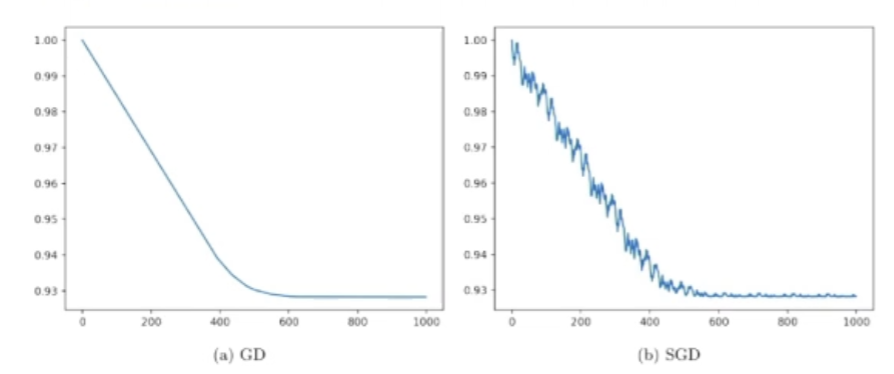
\includegraphics[width=0.75\linewidth]{images/sgd_vs_gd.png}

When we use GD, at each iteration, we change $\bar{\theta}$ based on the gradient of the loss function on the entire dataset. Barring any issues with step size ($\eta$), this would cause our epirical risk to decrease at every iteration, since we take into account the loss at every datapoint. Since the SGD algorithm only looks at the gradient of our loss function at one specific point, we won't always be decreasing overall risk when we consider our entire dataset. Thus, when we graph the empirical risk as number of iterations increase, we see that the GD algorithm is a smooth curve towards 0 and SGD is a spiky curve that still tends towards 0 but will occasionally increase in error. \\

In practice, we usually use an algorithm between GD and SGD, which is called mini-batch SGD. In this algorithm, you compute the gradient based on a subset of the entire training set.

\section{Linear Regression}

Labels of a supervised learning question could be discrete or continuous.
\begin{itemize}
	\item Discrete labels: classification
	\item Continuous labels: regression
\end{itemize}

In linear regression, often times we are looking for a function $f: \R^d \rightarrow \R$ where $f \in \mathcal{F}$. For many classification problems, we will restrict the possible functions that we get to specific classes of functions (i.e., quadratic, linear, etc.).\\

A linear regression function is simply a linear function of the feature vector:
\[ f(\bar x, \bar{\theta}, b) = \bar{\theta} \cdot \bar x + b \]

Learning task: Choose parameters in response to training set

\[ S_n = \{ \bar{x}^{(i)}, y^{(i)} \}_{i=1}^n \quad \bar x^{(i)} \in \R^d \quad y^{(i)} \in \R \]

\subsection{Empirical risk for Linear Regression}

\[ R_n(\bar{\theta}) = \frac 1 n \sum_{i=1}^n Loss(y^{(i)} - (\bar{\theta} \cdot \bar{x}^{(i)})) \]

\textbf{Note:} The loss for Linear Regression is almost exactly the same as linear classification, except you care less about the sign of the predicted label and more about the pure value. This is why in the loss function, we see $y^{(i)} - (\bar{\theta} \cdot \bar x^{(i)})$ instead of our usual $y^{(i)}(\bar{\theta} \cdot \bar x^{(i)})$, which was more useful when we cared only about sign.

\subsection{Least Squares Loss function}

Squared Loss: $Loss(z) = \frac {z^2} 2$\\

Idea: Permit small discrepancies and heavily penalize large deviations

\[ R_n(\bar{\theta}) = \frac 1 n \sum_{i=1}^n \frac {(y^{(i)} - (\bar{\theta} \cdot \bar{x}^{(i)}))^2} 2 \]

\begin{algorithm}
	\caption{Linear Regression Using Stochastic Gradient Descent With Squared Loss}
	\begin{algorithmic}
		\State $k \gets 0$, $\bar{\theta}^{(0)} \gets \bar{0}$
		\While{convergence criteria is not met}
		\State randomly shuffle points
		\For{$i = 1, \dots, n$}
		\State $\bar{\theta}^{(k+1)} \gets \bar{\theta}^{(k)} - \eta_k \nabla_{\bar{\theta}}Loss_{sqd}(y^{(i)} - (\bar{\theta} \cdot \bar{x}^{(i)}))|_{\bar{\theta} = \bar{\theta}^k}$
		\State $k \gets k + 1$
		\EndFor
		\EndWhile
	\end{algorithmic}
\end{algorithm}
After doing some computation
\[
	\begin{aligned}
		\nabla_{\bar{\theta}} Loss_{sqd}(y^{(i)} - (\bar{\theta}^{(k)} \cdot \bar x^{(i)})) &= \nabla_{\bar{\theta}} \frac{(y^{(i)} - (\bar{\theta} \cdot \bar{x}^{(i)}))^2} 2\\
		&= \frac {2 (y^{(i)} - \bar{\theta} \cdot \bar{x}^{(i)})} 2 (-\bar{x}^{(i)})\\
		&= (y^{(i)} - \bar{\theta} \cdot \bar{x}^{(i)})(-\bar{x}^{(i)})
	\end{aligned}
\]
We get 
\begin{algorithm}
	\caption{Linear Regression Using Stochastic Gradient Descent With Squard Loss (updated)}
	\begin{algorithmic}
		\State $k \gets 0$, $\bar{\theta}^{(0)} \gets \bar{0}$
		\While{convergence criteria is not met}
		\State randomly shuffle points
		\For{$i = 1, \dots, n$}
		\If{$(y^{(i)} - \bar{\theta}^{(k)}\cdot \bar{x}^{(i)})\bar{x}^{(i)} \ne 0$}
		\State $\bar{\theta}^{(k+1)} \gets \bar{\theta}^{(k)} + \eta_k (y^{(i)} - \bar{\theta} \cdot \bar{x}^{(i)})\bar{x}^{(i)}$
		\State $k \gets k + 1$
		\EndIf
		\EndFor
		\EndWhile
	\end{algorithmic}
\end{algorithm}

If we instead wanted to use GD, we would have the following function:

\begin{algorithm}
	\caption{Linear Regression Using Gradient Descent With Squard Loss}
	\begin{algorithmic}
		\State $k \gets 0$, $\bar{\theta}^{(0)} \gets \bar{0}$
		\While{convergence criteria is not met}
		\State $\bar{\theta}^{(k+1)} \gets \bar{\theta}^{(k)} + \frac {\eta_k} {n} \sum_{i = 1}^{n} (y^{(i)} - \bar{\theta}^{(k)} \cdot \bar{x}^{(i)})\bar{x}^{(i)}$
		\State $k \gets k + 1$
		\EndWhile
	\end{algorithmic}
\end{algorithm}

\newpage

\part{Lecture 5}

Last lecture we began talking about linear regression. The difference between linear classification and linear regression boils down to our label set. If our labels belong to a discrete set, then it is a linear classification problem. If our labels belong to a continuous set, then it is a linear regression problem. In a linear regression problem, we are trying to find 

\[ f(\bar x, \bar{\theta}, b) = \bar{\theta} \cdot \bar x + b \quad \text{where} \quad f: \R^d \rightarrow \R, \bar x \in \R^d\]


So that given a new feature vector $\bar{x}'$, we can predict its label $y'$.

\section{Closed form solution for Empirical Risk with Squared Loss}
\[ R_n(\bar{\theta}) = \frac 1 n \sum_{i=1}^n \frac {(y^{(i)} - (\bar{\theta} \cdot \bar{x}^{(i)}))^2} 2 \]

\begin{enumerate}
	\item Find gradient wrt $\bar {\theta}$
	\item Set it to zero and solve for $\bar{\theta}$
\end{enumerate}

\[
	\begin{aligned}
		\nabla_{\bar{\theta}} R_n(\bar{\theta}) &= -\frac 1 n \sum_{i=1}^n \bar{x}^{(i)}y^{(i)} + \frac 1 n \sum_{(i=1)}^n (\bar{\theta} \cdot \bar{x} ^{(i)}) \bar{x}^{(i)}\\
		\nabla_{\bar{\theta}} R_n(\bar{\theta}) |_{\bar{\theta} = \bar{\theta}^*} &= 0\\
																																						 &= -\frac 1 n \sum_{i=1}^n \bar{x}^{(i)}y^{(i)} + \frac 1 n \sum_{(i=1)}^n \bar{x} ^{(i)} (\bar{x}^{(i)})^T \bar{\theta}^* \\
	\end{aligned}
\]
Let

\[ A = \frac 1 n \sum_{(i=1)}^n \bar{x} ^{(i)} (\bar{x}^{(i)})^T, \quad \bar{b} = \frac 1 n \sum_{i=1}^n \bar{x}^{(i)}y^{(i)} \]

Then to get 
\[ \nabla_{\bar{\theta}} R_n(\bar{\theta}) |_{\bar{\theta}} = 0 \]
we simply set
\[ \bar{\theta}^* = A^{-1}\bar{b} \]

To find a nicer computation using linear algebra and our feature + label vectors, we do the following 

\[. 
	\begin{aligned}
		X &= [\bar{x}^{(1)}, \dots, \bar{x}^{(n)}]^T\\
			&= 
			\begin{bmatrix}
				x_1^{(1)} & \cdots & x_d^{(1)}\\
				\vdots & \ddots & \vdots\\
				x_1^{(n)} & \cdots & x_d^{(n)}
			\end{bmatrix}\\
		y &= 
		\begin{bmatrix}
			y^{(1)}\\
			\vdots\\
			y^{(n)}
		\end{bmatrix}
	\end{aligned}
\]
Then
\[ 
	\begin{aligned}
		A &= \frac 1 n \sum_{(i=1)}^n \bar{x} ^{(i)} (\bar{x}^{(i)})^T\\
			&= \frac 1 n X^TX\\
		\bar{b} &= \frac 1 n \sum_{i=1}^n \bar{x}^{(i)}y^{(i)}\\
						&= \frac 1 n X^T\bar{y}
	\end{aligned}
\]
Which gives us
\[ 
	\bar{\theta}^* = (X^TX)^{-1}X^T\bar{y}
\]
that exactly minimizes our Empirical Risk with Squared Loss.\\

We don't always use this closed form solution for a couple reasons. One reason is that it might be more efficient to use SGD rather than calculating the closed form solution. Since the closed form solution requires solving for the inverse of a matrix, this could take a very long time, or it could be impossible.\\

Remember, a matrix is not invertible if its determinant is zero, making it a singularity. This happens when its rows/columns are dependen, meaning information is lost and you can't uniquely reverse the transformation to get back the original input.

To solve this, we can do either of the following:

\begin{enumerate}
	\item Identify and remove offending features. Since you are the one deciding which elements are in a feature vector, you can remove dependent rows/columns. This is often hard and is very hands on.
	\item Use regularization. This is more simple and hands off way.
\end{enumerate}

\section{Brief Digression Back to Classification}

Some classification questions are much better classified using a higher dimensional shape, like a circle or a curve. Turns out, we can use the same algorithm as before to find these boundaries.\\

Lets assume that we want to learn a circlular boundary with center (2, 2) and radius 1. We need to find the following formula:

\[ 
	\begin{aligned}
		(x_1 - 2)^2 + (x_2 - 2)^2 &= 1^2\\
		x_1^2 - 4x_1 + 4 + x_2^2 - 4x_2 + 4 &= 1\\
		x_1^2 + x_2^2 - 4x_1 - 4x_2 + 7 &= 0
	\end{aligned}
\]

Which can be rewritten in matrices as:

\[ 
	\begin{bmatrix}
		x_1^2\\
		x_2^2\\
		x_1\\
		x_2\\
		1
	\end{bmatrix}
	\cdot
	\begin{bmatrix}
		1\\
		1\\
		-4\\
		-4\\
		7
	\end{bmatrix}
\]

To do this, we introduce \emph{feature maps}. In this case we have the following feature map:

\[
	\phi(\bar x) = 
	\begin{bmatrix} 
		 x_1^2\\
		 x_2^2\\
		 x_1\\
		 x_2\\
		 1
	\end{bmatrix}
\]

Which simple takes a two dimensional vector and maps it to a five dimensional space. We have seen this before when transiotioning from perceptron to perceptron with offset. We had a feature map that mapped a two dimensional input $[x_1, x_2]^T$ to a three dimensional space, specificall $[1, x_1, x_2]^T$.\\

Similar to before, our goal is to find $\bar{\theta}$ that would classify our dataset the best. In this example, $\bar{\theta} = [1, 1, -4, -4, 7]$.\\

Our final classifier would be $sign(\bar{\theta} \cdot \phi(\bar x))$\\

Visually, our feature map takes our feature vector from a lower dimensional space to a higher dimensional space and we find $\bar{\theta}$ in this higher dimensional space. When we remap all of our datapoints and $\bar{\theta}$ back to our lower dimensional space, we get something that might look very different from a line.\\

Here is what our GD and SGD for linear regression with squared loss function would look like if we wanted to solve for higher dimensional shapes.

\[ \phi: \R^d \rightarrow \R^p, \quad \text{Input: } \{(\bar{x}^{(i)}, y^{(i)})\}_{i=1}^n \rightarrow \{ (\phi (\bar{x}^{(i)}), y^{(i)}) \}_{i=1}^n\]

\begin{algorithm} \label{alg:GD For Higher Dimensions}
	\caption{Stochastic Gradient Descent With Squard Loss For Higher Dimensions}
	\begin{algorithmic}
		\State $k \gets 0$, $\bar{\theta}^{(0)} \gets \bar{0}$
		\While{convergence criteria is not met}
		\State $\bar{\theta}^{(k+1)} \gets \bar{\theta}^{(k)} + \frac {\eta_k} {n} \sum_{i=1}^n (y^{(i)} - \bar{\theta} \cdot \phi(\bar{x}^{(i)}))\phi(\bar{x}^{(i)})$
		\State $k \gets k + 1$
		\EndWhile
	\end{algorithmic}
\end{algorithm}

\begin{algorithm} \label{alg:SGD For Higher Dimensions}
	\caption{Stochastic Gradient Descent With Squard Loss For Higher Dimensions}
	\begin{algorithmic}
		\State $k \gets 0$, $\bar{\theta}^{(0)} \gets \bar{0}$
		\While{convergence criteria is not met}
		\State randomly shuffle points
		\For{$i = 1, \dots, n$}
		\If{$(y^{(i)} - \bar{\theta}^{(k)} \cdot \phi(\bar{x}^{(i)}))\phi(\bar{x}^{(i)}) \ne 0$}
		\State $\bar{\theta}^{(k+1)} \gets \bar{\theta}^{(k)} + \eta_k (y^{(i)} - \bar{\theta} \cdot \phi(\bar{x}^{(i)}))\phi(\bar{x}^{(i)})$
		\State $k \gets k + 1$
		\EndIf
		\EndFor
		\EndWhile
	\end{algorithmic}
\end{algorithm}


\section{Regression with Regularization}

Now that we have this feature map, we have a lot of power in our hands. Theoretically, if we have $n$ datapoints, we could perfectly fit a shape to our dataset. However, this probably isn't a good idea for two reasons. 
\begin{enumerate}
	\item It would be much more computationally expensive since you would need to feature map each feature map to a higher dimension, and you would need to do matrix arithmetic with (often much) higher dimensional matrices which could increase compution drastically.
	\item Since the goal of our shape is to be able to generalize to more data points, and overfitting to the dataset does not seem like it would do a good job with respect to our goal.
\end{enumerate}
To prevent overfitting, we introduce a new term in addition to our empirical risk function $R_n(\bar{\theta})$ to calculate our loss. This term is dependent on how complex our model is and is called the regularization term $\lambda Z(\bar{\theta})$, where $\lambda \ge 0$.\\

\textbf{Idea:} prefer a simpler hypothesis

\begin{itemize}
	\item will push parameters towards some default value (typically zero)
	\item resists setting parameters away from default value when data weakly tells us otherwise
\end{itemize}

Our new ridge loss function look like:

\[ J_{n,\lambda} (\bar{\theta}) = \lambda Z(\bar{\theta}) + R_n(\bar{\theta}) \]

\subsection{What should $Z(\bar{\theta})$}

Desirable characteristics:
\begin{itemize}
	\item should force components of $\bar{\theta}$ to be small (close to zero)
	\item Convex, Smooth
\end{itemize}

A popular choice
\begin{itemize}
	\item $\l_p norms$
	\item Let's use $\l_2$ norm as the penalty function
\end{itemize}

L2 regularization: $Z(\bar{\theta}) = \frac {||\bar{\theta}||^2} 2$\\
Squared loss: $R_n(\bar{\theta}) = \frac 1 n \sum_{i=1}^n \frac {(y^{(i)} - (\bar{\theta} \cdot \bar{x}^{(i)}))^2} 2$

So our complete ridge loss function is:

\[ J_{n,\lambda} (\bar{\theta}) = \lambda \frac {||\bar{\theta}||^2} 2 + \frac 1 n \sum_{i=1}^n \frac {(y^{(i)} - (\bar{\theta} \cdot \bar{x}^{(i)}))^2} 2 \]

\subsection{Ridge Loss Closed form solution}

Similar to before when we were trying to find the closed form solution to our squared loss function, to find the closed form solution to our Ridge Loss function, we do the following:

\begin{enumerate}
	\item Find gradient wrt $\bar{\theta}$
	\item Set it to zero and solve for $\bar{\theta}$
\end{enumerate}

\[
	\begin{aligned}
		\nabla_{\bar{\theta}} J_{n, \lambda} &= 0\\
																				 &= \nabla_{\bar{\theta}} \left(\lambda \frac {||\bar{\theta}||^2} 2 + \frac 1 n \sum_{i=1}^n \frac {(y^{(i)} - (\bar{\theta} \cdot \bar{x}^{(i)}))^2} 2\right)\\
																				 &= \nabla_{\bar{\theta}} \left(\lambda \frac {||\bar{\theta}||^2} 2\right) + (-b + A \bar{\theta})\\
																				 &= \lambda \bar{\theta} + A\bar{\theta} - b\\
		(\lambda I + A)\bar{\theta} &= b\\
		\bar{\theta} &= (\lambda I + A)^{-1}b\\
								 &= (\lambda' I + X^TX)^{-1}X^T \bar y
	\end{aligned}
\]

We can always find this value for theta as long as $\lambda > 0$ because $(\lambda' I + X^TX)^{-1}$ is always invertible when $\lambda > 0$.

\section{Classification with Regularization}

You can apply a similar idea of regularization to classifiers. A lot of the times, we don't only want a boundary that perfectly classifies each of our datapoints. We would also like our boundary to maximize the margins between our boundary and the datapoints so that it is less sensitive to noise. The function we would like to minimize is the following:

\[SVM = \lambda \frac {||\bar{\theta}||^2} 2 + \frac 1 n \sum_{i=1}^n max(1 - y^{(i)}(\bar{\theta} \cdot \bar{x}^{(i)}), 0) \]

This function is called the Soft margin SVM, solving for $\bar{\theta}$ that would minimize it turns out to maximize the margins.

\part{Lecture 6 - Kernels}

So far, we have benn talking about algorithms try to find a good value for $\bar{\theta}$. Eventually, we can use this $\bar{\theta}$ to predict the label for $\bar x$ by calculating $\bar{\theta} \cdot \bar x$.\\

Our most recent (and most advanced/general) algorithm \ref{alg:SGD For Higher Dimensions} involved using a feature map $\phi$ to raise our feature vectors to a higher dimension $\R^p$ and taking the dot product between these higher dimensional feature vectors $(\phi(\bar x^{(i)}) \cdot \phi(\bar x^{(j)}))$. This would result back into a number in $\R$. Sometimes, $(\phi(\bar x^{(i)}) \cdot \phi(\bar x^{(j)}))$ can be computed much more efficiently than searately computing $\phi(\bar x^{(i)})$ and $\phi(\bar x^{(j)})$.

\section{Kernels}

Each \emph{valid kernel} has an associated feature mapping:

\[ K(\bar u, \bar v) = \phi(\bar u) \cdot \phi(\bar v)\]

where

\[ \phi: \R^d \rightarrow \R^p, \quad K: \R^d \times \R^d \rightarrow \R\]

\subsection{Quadratic kernel}

Consider a Feature Map $\phi(\bar u) = [u_1^2, u_2^2, \sqrt 2 u_1u_2]^T$ for $\bar{u} \in \R^2$.\\
Here, $\phi: \R^2 \rightarrow \R^3$

\[ 
	\begin{aligned}
		\phi(\bar u) \cdot \phi(\bar v) &= [u_1^2, u_2^2, \sqrt 2 u_1u_2]^T \cdot [v_1^2, v_2^2, \sqrt 2 v_1v_2]^T\\
																		&= u_1^2v_1^2 + u_2^2v_2^2 + 2u_1u_2v_1v_2\\
																		&= (\bar u \cdot \bar v)^2
	\end{aligned}
\]

Kernel $K(\bar u, \bar v) = (\bar u \cdot \bar v)^2 = \phi(\bar u) \cdot \phi(\bar v)$

\part{Leacture 7}

\subsection{Kernel Trick with Gradient Descent}

Notice a very important aspect of our definition of a valid kernel. It can find the dotproduct of two vectors in $\R^d$. When we take a look at our update step in our gradient descent algorithm:

\[
	\bar{\theta}^{(k+1)} \gets \bar{\theta}^{(k)} + \frac {\eta_k} {n} \sum_{i=1}^n (y^{(i)} - \bar{\theta} \cdot \phi(\bar{x}^{(i)}))\phi(\bar{x}^{(i)})
\]

Notice that we only ever take the dot product between $\bar{\theta}$ and $\bar{x}^{(i)}$. We can't use a kernel here because $\bar{\theta}$ starts off in $\R^p$ and has no form in $\R^d$. In order to use a kernel, we need to rewrite our update so that we take the dot product between $\phi(\bar{x}^{(i)})$ and $\phi(\bar{x}^{(j)})$.

\subsubsection{Derivation of Kernel Trick}

\begin{itemize}
	\item Update Step:
		\[
			\bar{\theta}^{(k+1)} \gets \bar{\theta}^{(k)} + \frac {\eta_k} {n} \sum_{i=1}^n (y^{(i)} - \bar{\theta} \cdot \phi(\bar{x}^{(i)}))\phi(\bar{x}^{(i)})
		\]
	\item Assume $\bar{\theta}^{(0)} = \bar{0}$
	\item Define $\gamma_i^{(k)} = y^{(i)} - \bar{\theta}^{(k)} \cdot \bar x^{(i)}$, \quad $\alpha_i^{(k+1)} = \alpha_i^{(k)} + \frac{\eta_k}n \gamma_i^{(k)}$, \quad $\alpha_i^{(0)} = 0$
	\item Then to find $\bar{\theta}^{(1)}$, we find
		\[ 
			\begin{aligned}
				\bar{\theta}^{(1)} &= \bar{\theta}^{(0)} + \frac {\eta_0} n \sum_{i=1}^n((y^{(i)} - \bar{\theta}^{(0)} \cdot \bar{x}^{(i)}) \bar{x}^{(i)})\\
													 &= \frac{\eta_0}n \sum_{i = 1}^n (\gamma_i^{(0)} \bar{x}^{(i)})\\
													 &= \sum_{i = 1}^n (\alpha_i^{(1)} \bar{x}^{(i)})
			\end{aligned}
		\]
	\item To find $\bar{\theta}^{(2)}$:
		\[ 
			\begin{aligned}
				\bar{\theta}^{(2)} &= \bar{\theta}^{(1)} + \frac{\eta_1}n \sum_{i=1}^n (\gamma_i^{(1)} \bar{x}^{(i)})\\
													 &= \sum_{i=1}^n (\alpha_i^{(1)} + \frac{\eta_1}n \gamma_i^{(1)}) \bar{x}^{(i)}\\
													 &= \sum_{i=1}^n (a_i^{(2)} \bar{x}^{(i)})
			\end{aligned}
		\]
		\item Thus
			\[ \bar{\theta}^{k} = \sum_{i=1}^n (a_i^{(k)} \bar{x}^{(i)}) \]
		\item Also notice
			\[ 
				\begin{aligned}
					\alpha_i^{(k+1)} &= \alpha_i^{(k)} + \frac{\eta_k}n \gamma_i^{(k)}\\
													 &= \alpha_i^{(k)} + \frac{\eta_k}n (y^{(i)} - \bar{\theta}^{(k)} \cdot \bar{x}^{(i)})\\
													 &= \alpha_i^{(k)} + \frac{\eta_k}n \left( y^{(i)} - \left( \sum_{j=1}^n \alpha_j^{(k)} \bar{x}^{(j)} \right) \cdot \bar{x}^{(i)} \right)\\
													 &= \alpha_i^{(k)} + \frac{\eta_k}n \left( y^{(i)} - \sum_{j=1}^n \left(  \alpha_j^{(k)} \bar{x}^{(j)} \cdot \bar{x}^{(i)} \right) \right)
				\end{aligned}
			\]
		\item If each feature $\bar{x}^{(i)}$ was mapped to a higher dimension using $\phi$, and if $K$ was a valid kernel such that $K(\bar u, \bar v) = \phi(\bar u) \cdot \phi(\bar v)$, we get
			\[ 
				\begin{aligned}
					\alpha_i^{(k+1)} &= \alpha_i^{(k)} + \frac{\eta_k}n \left( y^{(i)} - \sum_{j=1}^n \left(  \alpha_j^{(k)} \bar{x}^{(j)} \cdot \bar{x}^{(i)} \right) \right)\\
													 &= \alpha_i^{(k)} + \frac{\eta_k}n \left( y^{(i)} - \sum_{j=1}^n \left( \alpha_j^{(k)} K(\bar{x}^{(j)}, \bar{x}^{(i)}) \right) \right)
				\end{aligned}
			\]
		\item Since 
			\[ \bar{\theta}^{k} = \sum_{i=1}^n (a_i^{(k)} \bar{x}^{(i)}) \]
			The prediction on $\bar x$ becomes
			\[ \sum_{i=1}^n \alpha_i^{(k)}(K(\bar{x}^{(i)}, \bar{x})) \]
		\item Final note: To reason through our formula to calculate $\alpha_i^{(k+1)}$, we can compare it to the prediction formula above. Observe that

			\[
				\alpha_i^{(k+1)} = \alpha_i^{(k)} + \frac{\eta_k}n \left( y^{(i)} - \sum_{j=1}^n \left( \alpha_j^{(k)} K(\bar{x}^{(j)}, \bar{x}^{(i)}) \right) \right)
			\]

			Has exactly the term for a prediction of $\bar x^{(i)}$:

			\[ \sum_{j=1}^n \alpha_j^{(k)}(K(\bar{x}^{(j)}, \bar{x}^{(i)})) \]

			Thus, our update for $\alpha_i^{(k+1)}$ is exactly $\alpha_i^{(k)}$ plus the difference between the given label $y^{(i)}$ and our predicted label $\sum_{j=1}^n \alpha_j^{(k)}(K(\bar{x}^{(j)}, \bar{x}^{(i)}))$ (bar the step size).

\end{itemize}

This concludes our derivation of the kernel

\subsection{Examples of Valid Kernels}

Linear Kernel:
\[ K(\bar u, \bar v) = \bar u \cdot \bar v \]

Quadratic Kernel:
\[ K(\bar u, \bar v) = (\bar u \cdot \bar v + r)^2 \text{ with } r \ge 0 \]

RBF Kernel (aka Gaussian Kernel):
\[ K(\bar u, \bar v) = \exp(-\gamma ||\bar u - \bar v||^2) \text{ with } \gamma \ge 0 \]

The RBF Kernel is special because it's underlying feature map is infinite dimensional and is controlled by $\gamma$ (we can show this through the Taylor Series expansion of $e$). $\gamma$ scales the affect of higher dimensional terms, so higher gamma leads to more complex models.

\begin{itemize}
	\item Small $\gamma$: Larger influence, resulting in smoother decision boundaries. The function becomes more spread out, meaning data points can influence far-away regions.
	\item Large $\gamma$: Samller influence, resulting in more complex decision boundaries. The function becomes narrow, meaning each point only affects its immediate neighbors
\end{itemize}

\subsection{Kernel Algebra}

Let $K_1(\bar x, \bar z)$ and $K_2(\bar x, \bar z)$ be valid kernels, then the following are valid kernels:
\[ K (\bar x, \bar z) = K_1(\bar x, \bar z) + K_2(\bar x, \bar z) \quad \text{sum}\]
\[ K (\bar x, \bar z) = \alpha K_1(\bar x, \bar z), \quad \alpha > 0 \quad \text{scalar product}\]
\[ K (\bar x, \bar z) = K_1(\bar x, \bar z) K_2(\bar x, \bar z) \quad \text{product}\]

\subsection{Mercer's Theorem}

A function $K: \R^d \times \R^d \rightarrow \R$ is a valid kernel iff for any $\bar{x}^{(1)}, \dots, \bar{x}^{(n)}$ with $\bar{x}^{(i)} \in \R^d$ and finite $n$ the $n \times n$ matrix $G$ with $G_{ij} = K(\bar{x}^{(i)}, \bar{x}^{(j)})$ is \emph{positive-semidefinite}. That is, $G$ is

\begin{itemize}
	\item symmetric ($G = G^T$)
	\item $\forall z \in \R^n \quad z^TGz \ge 0$
\end{itemize}

In other words, a function is a valid kernel iff:

\begin{itemize}
	\item There exists a function $\phi(\cdot)$ such that $K(\bar x, \bar z) = \phi(\bar x) \cdot \phi(\bar z)$
	\item Symmetry: $K(\bar x, \bar z) = K(\bar z, \bar x)$
	\item Non-negative for a vector with itself: $K(\bar x, \bar x)$
\end{itemize}



\section{Classifiers in Practice}

\subsection{Training strategy}

Now that we have all the tools to create a model, we have to train our model in a strategic way. As we've said before, making our model too complex could lead to overfitting to our training dataset, which could lead to poor performance when testing our model on non-trained datapoints. We have already gone through a possible technique to prevent overfitting called regularization. To further prevent overfitting, we can split our training dataset into 3 parts:

\begin{itemize}
	\item Training dataset: these datapoints are used to train our model and should have less error/loss as our model gets more complex
	\item Validation dataset: these datapoints are used to determine how well our model works on datapoints that it wasn't tested on. The error on this dataset should be parabolic (high when the mdoel is very simple and too complex, and low when it find a good balence w.r.t the training dataset).
	\item Test dataset: Used at the end (probably only once per classification question) to determine the final efficacy of the model.
\end{itemize}

\subsection{Feature Selection}

\textbf{Motivation}

\begin{itemize}
	\item When you have few examples and a large number of features (i.e., $d >> n$) it becomes very easy to overfit your training data
	\item How can we remove uniformative features?
\end{itemize}

Different FS approaches:
\begin{enumerate}
	\item Filter
	\item Wrapped
	\item Embedded
\end{enumerate}

\subsubsection{Filter Approach}
\begin{itemize}
	\item rank features according to some metric (independent of learning algo)
	\item filter out features that fall below a certain threshold
\end{itemize}

Example metric: correlation with output/label

\textbf{Pearson's correlation}

\[  
	r_{x_j, y} = \frac {\sum_{i=1}^n (x_j^{(i)} - \tilde x_j)(y^{(i)} - \tilde y)} {\sqrt{\sum_{i = 1}^n (x_j^{(i)} - \tilde x_j)^2} \sqrt{\sum_{i=1}^n (y^{(i)} - \tilde y) ^2}} 
\]

\subsubsection{Wrapper Approach}
\begin{itemize}
	\item utilize learning algo to score subsets according to predictive power
	\item learning algorithm is ``wrapped" in a search algorithm
\end{itemize}

Both the Filter and Wrapper approach are heuristics that forces you to think critically on certain aspects of the entire model

\subsubsection{Embedded Methods}
\begin{itemize}
	\item Incorporate varaible selection as part of the training process
		\begin{itemize}
			\item Regularization with L1 or L2 norms
			\item When $\lambda$ is sufficiently large, the L1-norm penalty will shrink some parameters to zero, which gives us implicit (or embedded) feature selection
		\end{itemize}
	\item How do we choose hyperparameters like $\lambda$? We can choose a value for $\lambda$ and use k-fold Cross Validation
\end{itemize}

\subsection{k-fold Cross Validation}

Partition the dataset into $k$ subsets. Choose one of the subsets to be the validation set and the other $k-1$ subsets to be the training dataset. After training the model, test it on the validation set. Average the results over $k$ runs. This ensures that our model is less prone to varaince in validation set selection.

\subsection{Evaluating Classifiers}

\textbf{Common Performance Metrics}\\

\[
	\begin{aligned}
		\text{Classification Error}:& \quad FP+FN\\
		\text{Accuracy}:& \quad \frac {TP+TN}N\\\\
		\text{False Positive Rate}:& \quad \frac {FP} {TN+FP}\\
		\text{True Positive Rate}:& \quad \frac {TP}{TP+FN}\\\\
		\text{Sensitivity (Recall)}:& \quad TPR\\
		\text{Precision}:& \quad \frac{TP}{TP+FP}\\
		\text{Specificity}:& \quad \frac{TN}{TN+FP}\\\\
		\text{F1 Score}:& \quad \frac{2 * Precision * Sensitivity} {Precision + Sensitivity}
	\end{aligned}
\]

\part{Lecture 8}

\section{Decision Trees}

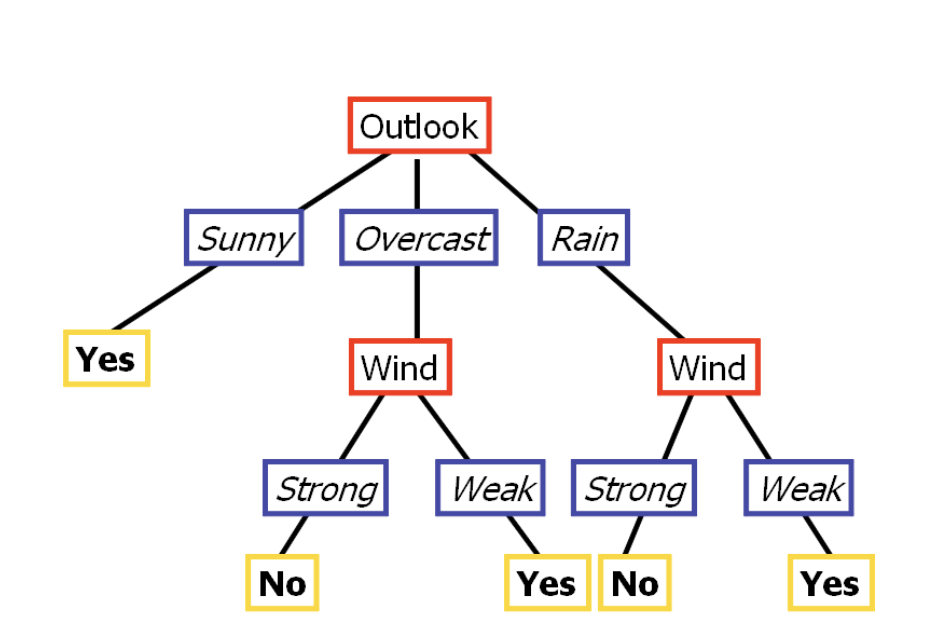
\includegraphics[width=0.75\linewidth]{images/decision_tree_example_1.png}

\subsection{Overview}

Decision Trees are a powerful class of model that have the following pros:

\begin{itemize}
	\item Iterpertability \& Transparency: The tree structure is easy to understand even for non-technical users. It is also provides a very clear train of thought that a user can apply when making decisions. 
	\item Effectively models complex patterns where features and outcomes aren't linearly related. Ex: Can perfectly classify the XOR dataset, whereas the linear classifiers could not.
\end{itemize}

\textbf{Definition:} 

\begin{itemize}
	\item Each internal node an attribute/feature $x_i$
	\item Each branch assigns a value $x_i = v$
	\item Each leaf assigns a class (binary or discrete) $\hat{y}_i$
\end{itemize}

\textbf{Goal}: Find the smallest decision tree that minimizes error

\begin{itemize}
	\item NP-hard question
	\item Idea: use a heuristics - greedy approach to picking ‘best’ attribute to split on
\end{itemize}

\subsection{Decision Tree: Greedy approacch} \label{sub:14.1}

\textbf{Idea:} Pick a split that leads to more certainty in classification\\

Ex: \begin{tabular}{|c|c|c|}
	\hline
	$x_1$ & $x_2$ & $y$\\
	\hline
	a & 1 & T\\
	\hline
	a & 1 & T\\
	\hline
	a & 2 & F\\
	\hline
	a & 1 & F\\
	\hline
	b & 2 & T\\
	\hline
	b & 2 & F\\
	\hline
\end{tabular}\\

In this case, you could first split on either $x_1$ or $x_2$. The following tables show the results of splitting on $x_1$ and $x_2$:\\

\begin{tabular}{|c|c|c|}
	\hline
	$x_1$ & T & F\\
	\hline
	a & 1/2 & 1/2\\
	\hline
	b & 1/2 & 1/2\\
	\hline
\end{tabular} \quad
\begin{tabular}{|c|c|c|}
	\hline
	$x_2$ & T & F\\
	\hline
	1 & 2/3 & 1/3\\
	\hline
	2 & 1/3 & 2/3 \\
	\hline
\end{tabular}\\

Intuitively, splitting on $x_2$ gives us a better split since the value of $x_2$ actually helps us with our decision of $y$.

\subsection{Measuring Uncertainty: Shannon Entropy}

We need a function that meansures the uncertainty of our labels in our training dataset. Later, once we generalize this to be able to compare uncertainty between splits of a decision tree, this will be useful for our greedy algorithm mentioned above. For binary classification, here are a couple of properties that we want our function to exhibit:

\begin{enumerate}[label=(\alph*)]
	\item Entropy is at its peak when $P_{\oplus}$ (the percentage of positive labels) or, equivalently, $P_{\ominus}$ is equal to 0.5.
	\item Entropy is at its lowest, 0, when $P_{\oplus}$ (or, equivalently, $P_{\ominus}$) is equal to 0 or 1.
	\item Entropy is equivalent when $P_{\oplus}$ is equal to $\frac 1 3$ and $\frac 2 3$, or in other words, the function is symmetric.
\end{enumerate}

Shannon's Entropy is defined as follows:

\[ Entropy(S_n) = -p_{\oplus}\log_2p_{\oplus} - p_{\ominus}\log_2p_{\ominus}\]

\textbf{Note}: Assumy by convention $0 \log 0 = 0$\\

The function, when graphed, look like this:

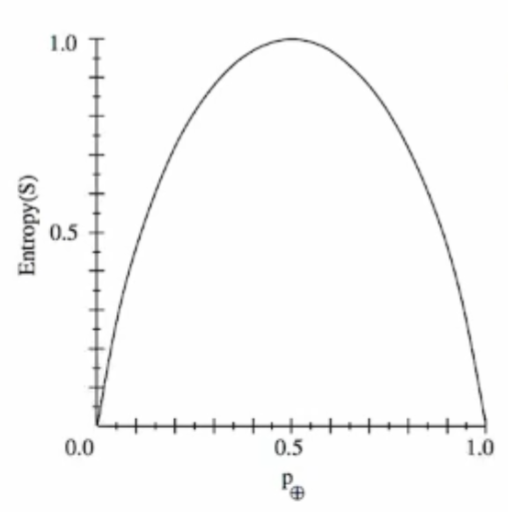
\includegraphics[width=0.25\linewidth]{images/shannon_entropy.png}

\subsection{Entropy and Conditional Entropy}

In general, for $k$-class classification, the uncertainty in the class label $Y$ becomes

\[ H(Y) = -\sum_{i=1}^k Pr(Y=y_i) \log_2 Pr(Y=y_i) \]

If we wanted to know the uncertainty of a class label given that a specific feature $X$ took a particular value $x_j$, the formula becomes

\[ H(Y | X = x_j) = -\sum_{i=1}^k Pr(Y=y_i | X=x_j) \log_2 Pr(Y=y_i | X=x_j) \]

Finally, if we wanted to know the uncertainty of a class label given that you knew the value of a specific feature $X$, the formula becomes

\[ H(Y | X) = \sum_{j=1}^m Pr(X=x_j) H(Y|X=x_j) \]

\subsection{Information Gain}

The amount of information we learn about the class label $Y$, given a specific feature $X$, is given by the following formula:

\[ IG(X,Y) = H(Y) - H(Y|X) \]

Which, in words, means that the information gained from knowing a specific feature is the difference between the uncertainty before knowing the feature and the uncertainty after knowing the feature.

\begin{itemize}
	\item Supposed the feature $X$ and class label $Y$ are independent random varaibles. Then when finding the uncertainty of $Y$ given feature $X$, we get

		\[ H(Y | X = x_j) = -\sum_{i=1}^k Pr(Y=y_i) \log_2 Pr(Y=y_i) = H(Y) \]
		
		which makes

		\[ H(Y | X) = \sum_{j=1}^m Pr(X=x_j) H(Y) = H(Y) \]

		So $IG(X,Y) = 0$

	\item Supposed the class label $Y$ is completely dependent on $X$. Then $H(Y|X) = 0$ and so $IG(X,Y) = H(Y)$
\end{itemize}

\subsection{Learning Decision Trees}

In subsection \ref{sub:14.1}, we talked about a greedy approach to creating a decision tree that has 

\begin{enumerate}
	\item best classification
	\item minimum depth
\end{enumerate}

This approach followed these steps:

\begin{enumerate}
	\item start with an empty tree
	\item split on the ``best" feature
	\item recurse
\end{enumerate}

To elaborate on this algorithm, we say to find the best feature, we find the feature that results in the most information gain.

\[ 
	\begin{aligned}
		best\_feature &= arg max_j IG(X_j, Y)\\
									&= argmax_jH(Y) - H(Y|X_j)\\
									&= argmin_jH(Y|X_j)  
	\end{aligned}
\]

\subsection{Stopping Criterion}

Here are a few intuitive stopping criterias for creating our decision tree:

\begin{enumerate}
	\item When all records (datapoints) have the same label
	\item If all records have identical features (no further splits possible)
	\item If all attributes have zero IG. This is not a great approach for a couple reasons
		\begin{itemize}
			\item Could lead to overfitting to the training data.
			\item Could halt early and ignore potential iteractions between features. Consider the xor dataset \ref{tab:xor_data}.
				\begin{table}[h]
					\centering
					\caption{XOR dataset} 
					\vspace{2mm}
					\label{tab:xor_data}
					\begin{tabular}{|c|c|c|}
						\hline
						$x_1$ & $x_2$ & $y$\\
						\hline
						1 & 1 & 0\\
						\hline
						1 & 0 & 1\\
						\hline
						0 & 1 & 1\\
						\hline
						0 & 0 & 0\\
						\hline
					\end{tabular}
				\end{table}
				If you consider $x_1$ and $x_2$ separately, each would result in an information gain of 0. However, together, they would make a perfect classifier. The main issue with halting on zero information gain is because that would immediately assume that features don't rely on each other. This is because the greedy algorithm only considers the locally best feature by itself and doesn't persue and interactions between featues. 
		\end{itemize}
	\item When the decision tree reaches a maximum depth
	\item Measure performance on validation data. Halt if growing tree results in worse performance.
	\item Post-prune. Grow entire/full tree and then greedily remove nodes that affect validation error the least.
\end{enumerate}

Options 4-6 are effective at avoiding overfitting to the training dataset. Option 6 is interesting because it seems similar to option 5, but remember that because of our greedy algorithm, the IG gain or validation metric could get worse before it gets better due to interactions between labels. Take the XOR dataset \ref{tab:xor_data} as an example.

\subsection{Learning Decision Trees: Pseudocode}

\begin{algorithm} \label{Decision Tree: Greedy Algorithm}
\caption{Decision Tree: Greedy Algorithm}
\begin{algorithmic}
\Function{BuildTree}{$DS$}
		\If{$y^{(i)} = y$ for all examples in $DS$} \Comment{all labels are the same}
        \State \Return $y$
    \ElsIf{$\mathbf{x}^{(i)} = \mathbf{x}$ for all examples in $DS$} \Comment{all rows have same feature values}
        \State \Return majority label
    \Else
        \State $x_s = \arg\min_x H(y|x)$
        \For{each value $v$ of $x_s$}
            \State $DS_v = \{ \text{examples in } DS \text{ where } x_s = v \}$
            \State \Call{BuildTree}{$DS_v$}
        \EndFor
    \EndIf
\EndFunction
\end{algorithmic}
\end{algorithm}

For the recursive step, here is an example of what the algorithm would look like. Lets say we had the following data set

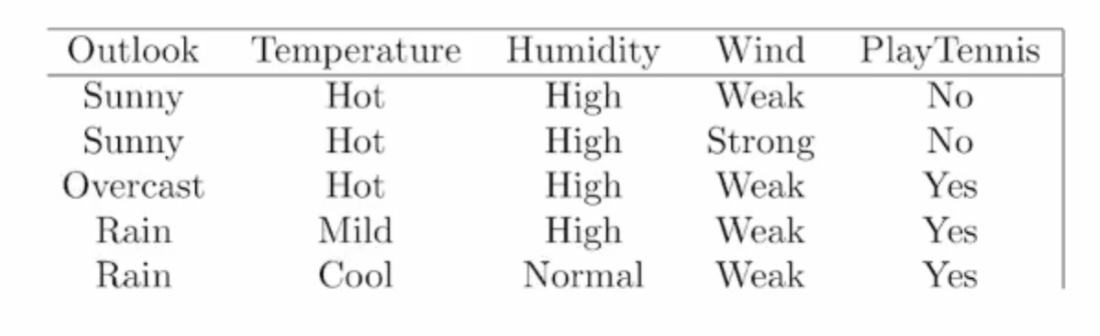
\includegraphics[width=0.75\linewidth]{images/decision_tree_example_3.png}

If we wanted to split on the ``Outlook" label, we would make 3 different $DS_v$ for each unique value of the outlook label:

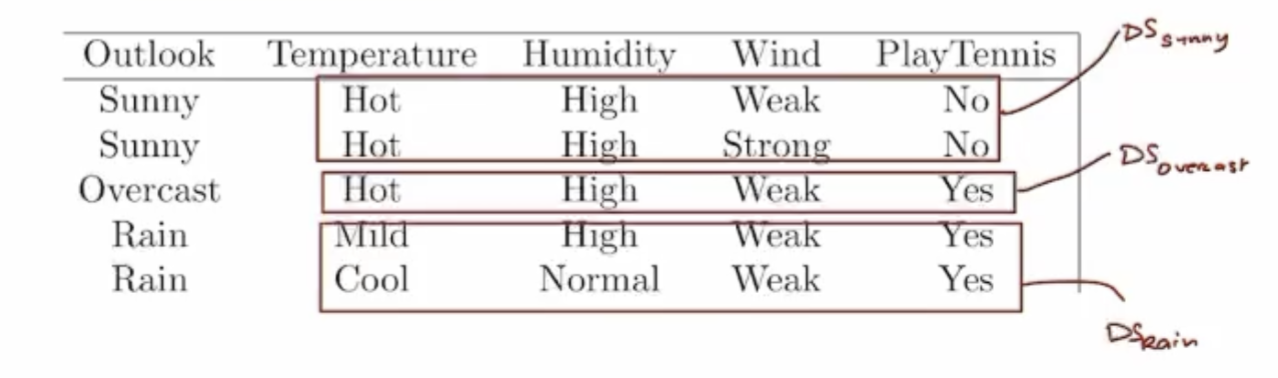
\includegraphics[width=0.75\linewidth]{images/decision_tree_example_4.png}

For each of the unique $DS_v$ ($DS_{sunny}, DS_{Overcast}, DS_{Rain}$), we would recursively call the BuildTree function on that $DS_v$ to build that branch of our decision tree.\\

\textbf{Note:} Observe that this algorithm does not necessarily make a symmetric decision tree (which is expected for a decision tree).

\textbf{Note 2:} This greedy algorithm \ref{Decision Tree: Greedy Algorithm} is still the most popular way to build a decision tree.

\section{Sources of Error}

\textbf{Goal:} Minimize generalization error

Sources of error:

\begin{itemize}
	\item bias (structural error). You usually get this from a model that is not complex enough to understand the underlying patterns in a training dataset. 
	\item variance (estimation error). You usually get this from a model that is too complex and sees noise as patterns in a training dataset.
	\item noise. Natural variance and non-certain choices in the problem that you can't really do anything about.
\end{itemize}

\subsection{Bias-Variance tradeoff}

\textbf{Estimation Error (variance)}
\begin{itemize}
	\item low variance $\rightarrow$ constant function
	\item high variance $\rightarrow$ high degree polynomial, RBF kernel 
\end{itemize}

\textbf{Structural Error (bias)}
\begin{itemize}
	\item low bias $\rightarrow$ Linear regression applied to linear data, RBF kernel 
	\item high bias $\rightarrow$ constant function, linear model applied to non-linear data
\end{itemize}

So far, the strategies that we know (i.e., tuning hyperparameters) only shift along the bias/variance tradeoff. We will learn a strategy that allows us to keep bias fixed while lowering variance.

\part{Lecture 9}

\section{Ensemble Methods}

\textbf{Goal:} decrease variance without increasing bias\\
\textbf{Idea:} average across multiple models to reduce variance.\\

But how do we learn different Decision Trees from an essentially deterministic algorithm?\\

\textbf{Idea 1:} Train Decision Trees on Split Dataset. \\

This idea is a great starting point, but there are a few problems. The main problem is that the training dataset gets smaller, so the model will tend to overfit even harder to the smaller datasets. Additionally, if you wanted a large number of decision trees, each model will get trained on less and less datapoints and likely result in increasingly more error.\\

\textbf{Idea 2:} Bootstrap Sampling. \\

Bootstap sampling is done by drawing uniformly at random (with replacement) from the training dataset to create a new training dataset with the same size as the original training dataset. You can prove that if the original testing dataset represented the true underlying distribution of global datapoints, so will the bootstrap samples.

\subsection{Bagging} \label{bagging}

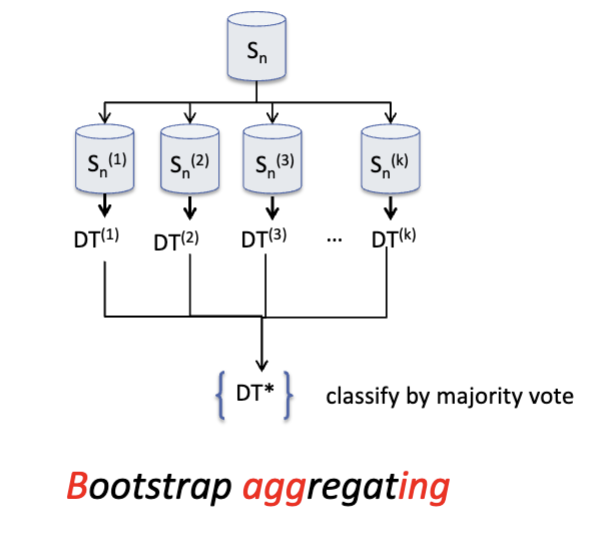
\includegraphics[width=0.75\linewidth]{images/bagging.png}

\textbf{Idea:} Using some method to get multiple datasets (ex, Bootstrap Sampling), generate multiple different models based on those datasets. On a new datapoint to classify, run the datapoint through each of the models and take the majority vote of what label they decide.\\

\textbf{Note:} $B$ is the number of models in our bag.\\

\textbf{Result:} As $B \rightarrow \infty$, missclassification rate $\rightarrow$ 0\\

\textbf{Assumptions:}
\begin{itemize}
	\item	each decision tree has a misclassification rate of better that 50\%
	\item classifiers are independent
\end{itemize}

Even though, theoreticlally, missclassification rate goes to zero as $B \rightarrow \infty$, prediction error rarely ever goes to zero. This happens for 2 main reasons:

\begin{itemize}
	\item	Bagging reduces variance (estimation error), but bias (structural error) may still remain
	\item Independence of classifiers is a strong assumption
\end{itemize}

\subsection{Random Forest Procedure}

\begin{algorithm} \label{Random Forest Procedure}
\caption{Random Forest Procedure}
\begin{algorithmic}
		\For{$b = 1, \dots, B$}
        \State draw bootstrap sample $S_n(b)$ of size $n$ from $S_n$
				\State grow decision tree $DT^{(b)}$
    \EndFor
		\State return Ensemble \{ $DT^{(1)}, \dots, DT^{(B)}$ \}
\end{algorithmic}
\end{algorithm}

[subprocedure for growing $DT^{(b)}$]
until stopping criteria are met, recursively repeat following steps for each node of tree:
\begin{enumerate}
	\item select $k$ features at random from $d$ features
	\item pick best feature to split on (using IG)
	\item split node into children
\end{enumerate}

The Random Forest Procedure is essentially the bagging ensemble method we talked about in subsection \ref{bagging}. The main difference is that to grow decision tree $DT^{(b)}$, we first select $k$ reatures at random from the entire $d$ features. This is done to make each classifier as independent from one another as possible, so that the ``Classifiers are independent" claim is stronger.

\subsection{Boosting}

Boosting is a family of ensemble methods that convert a collection of weak models (models that are only slightly better than random guessing, with a missclassification rate that must be $>$ 0.5) into a single, stronger model.

\section{AdaBoost}

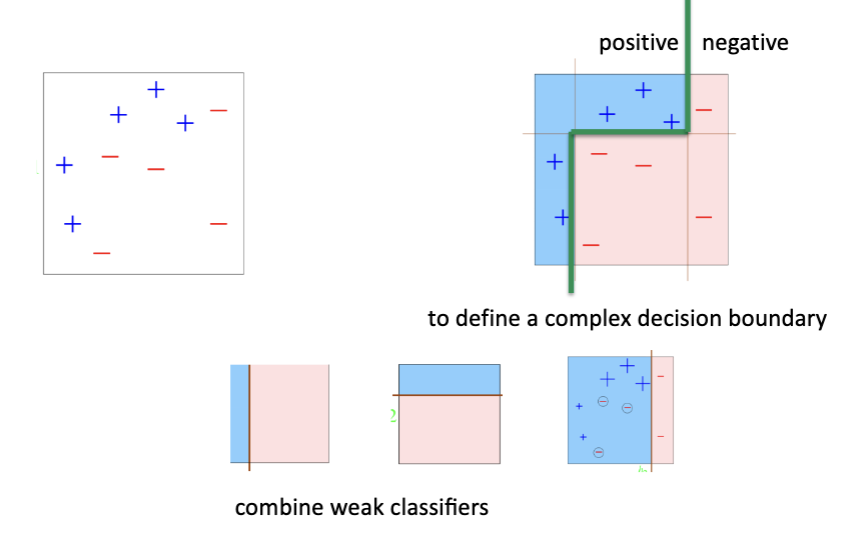
\includegraphics[width=0.75\linewidth]{images/adaboost.png}

Adaboost, short for Adaptive Boosting, belongs to the Boosting family of ensemble methods. It optimizes exponential loss:

\[ Loss_{exp}(z) = exp(-z) \]

The ensemble classifier that is learned is the following:

\[ h_M(\bar{x}) = \sum_{j=1}^M a_j h(\bar x; \bar{\theta}_j) \]

AdaBoost aims to minimize

\[ \sum_{i=1}^n Loss_{exp}(y^{(i)} h_m(\bar x ^{(i)})) \]

\subsection{Decision stups as a weak classifier}

Each $h(\bar x, \bar{\theta})$ is called a decision stub because its goal is to simply split the classification space by a single feature (depth 1 decision tree). 

\[ h(\bar x; \bar{\theta}) = sign(\theta_1 (x_k - \theta_0)) \]

where

\[ \bar{\theta} = (k, \theta_0, \theta_1) \in \R^3, \quad x \in \R^d \]

and 

\[ k \rightarrow \text{coordinate/feature}, \quad \theta_0 \rightarrow \text{position}, \quad \theta_1 \rightarrow \text{direction} \]

\subsection{AdaBoost: Example}

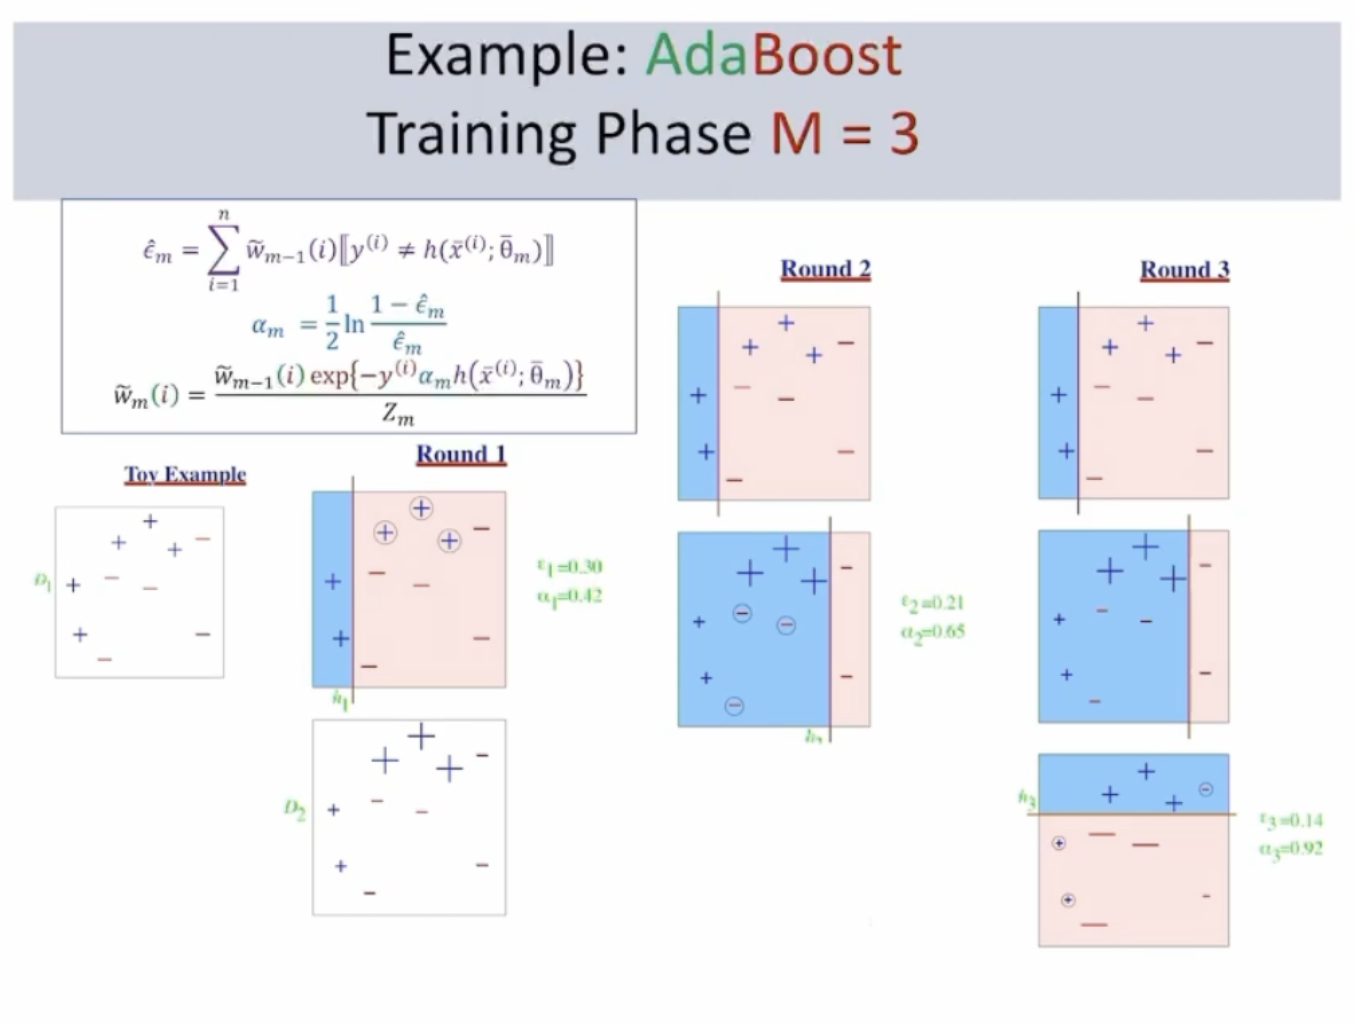
\includegraphics[width=0.75\linewidth]{images/adaboost_example_1.png}\\

\[ \hat{\epsilon}_m \rightarrow \text{error of mth classifier}, \quad \alpha_m \rightarrow \text{weight of mth classifier}, \quad \widetilde{w}_m(i) \rightarrow \text{weigh of mth datapoint} \]

\[ Z_m = \sum_{i=1}^{n} \widetilde{w}_{m}(i) \quad \text{(nomalization factor)} \]

Most interesting things about the formulas to focus on:

\begin{itemize}
	\item Missclassified points are increased in weight while correctly classified points are decreased in weight. This is done by the exp function inside of the calculation for $\widetilde{w}_m(i)$. If point i was correctly classified, then $sign(y^(i)) == sign(h(\bar{x}^{(i)}; \bar{\theta}_m))$ and $ -y^{(i)} \alpha_m h(\bar x^{(i)}; \bar{\theta}_m) $ is negative so $\exp\{ -y^{(i)} \alpha_m h(\bar x^{(i)}; \bar{\theta}_m) \}$ is small ($<1$). If point i was incorrectly classified, then $sign(y^(i)) \ne sign(h(\bar{x}^{(i)}; \bar{\theta}_m))$ and $ -y^{(i)} \alpha_m h(\bar x^{(i)}; \bar{\theta}_m) $ is positive so $\exp\{ -y^{(i)} \alpha_m h(\bar x^{(i)}; \bar{\theta}_m) \}$ is large ($>1$). 
	\item The error of the mth classifier is not only dependent on how many points the classifier correctly classifies, but also how how much the correctly classified points are weighted. 
	\item AdaBoost cannot solve all problems. Take, for example, the xor dataset \ref{tab:xor_data}. Since AdaBoost only allows for $\bar{\theta}$ to draw a line parallel to the $y$-axis or $x$-axis, it can only allows for a classification rate $=$ 0.5. One of our original assumptions for AdaBoost to work is that each weak classifier does slightly better than random guessing (missclassification rate $>$ 0.5). Since this is not true, $\alpha_m = \frac 1 2 \ln \frac {1/2} {1/2} = 0$, so the classifier has a weight of 0 and the procedure breaks.
	\item Weighted error relative to updated weights: 
		\[ \sum_{i=1}^n \widetilde{w}_m(i) [[y^{(i)} \ne h(\bar x^{(i)}; \bar{\theta}_m)]] \]
		is exactly 0.5. This means that in future iterations, when we are picking a weak classifier that does better than chance (missclassification rate $> 0.5$), we will never pick the same classifier ever again. Otherwise, the weighted error would equal $0.5$, which contradict our statement that the future classifier does better than chance.
\end{itemize}

\subsection{AdaBoost: Classify}

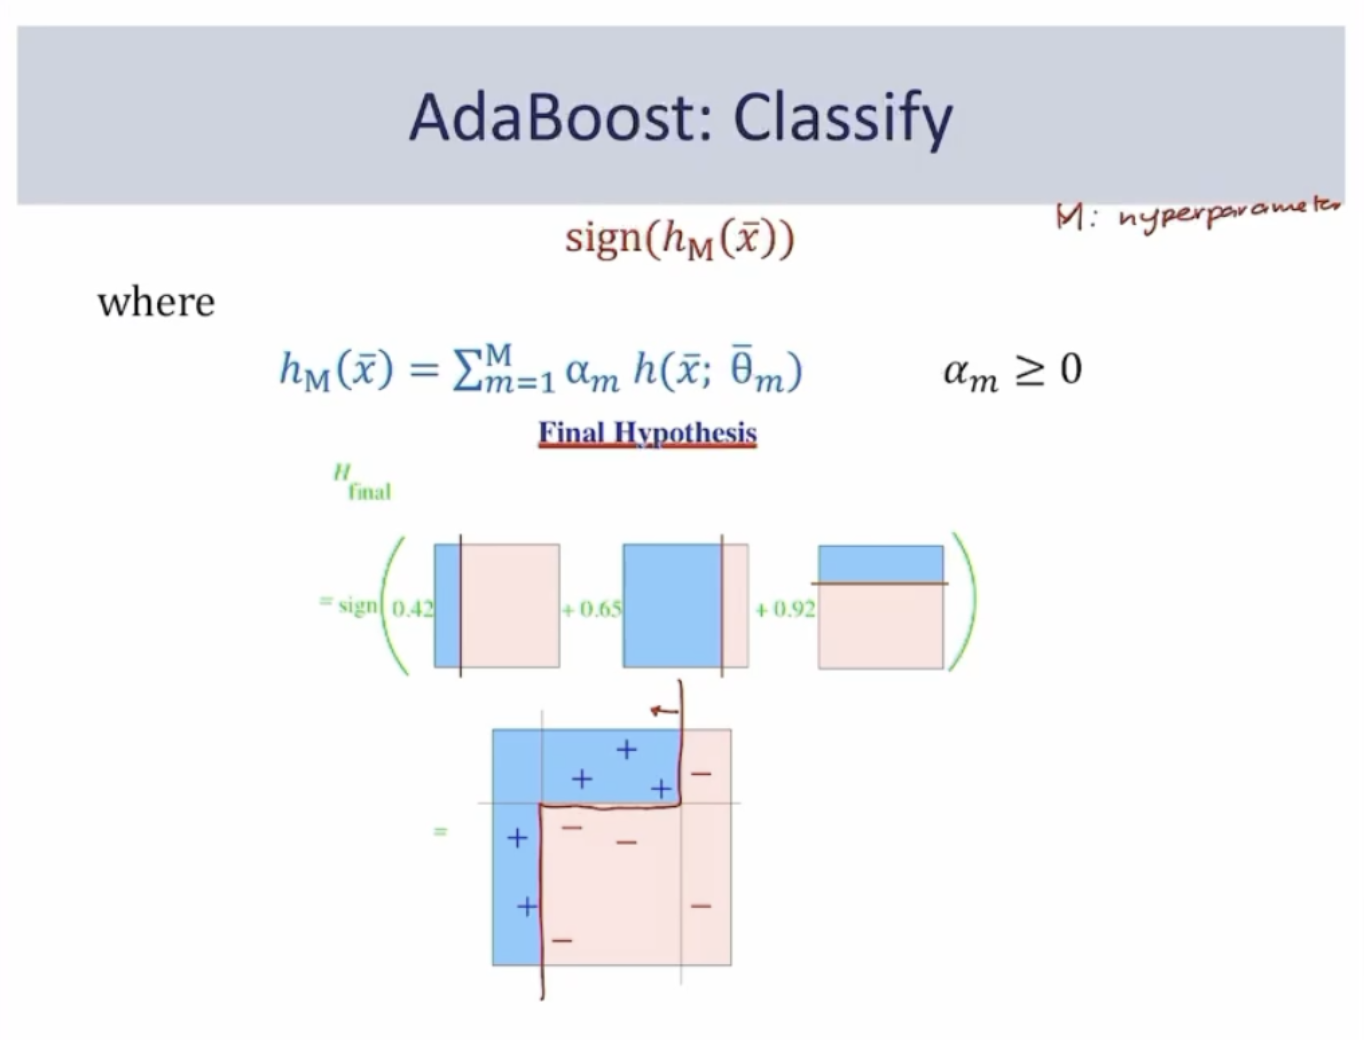
\includegraphics[width=0.75\linewidth]{images/adaboost_example_2.png}\\

\newpage

\subsection{AdaBoost Algorithm}

\begin{algorithm} \label{alg:AdaBoost}
\caption{AdaBoost}
\begin{algorithmic}
	\For{$i = 1, \dots, n$}
		\State $\widetilde{w}_0(i) = \frac 1 n$
	\EndFor
	\For{$m = 1, \dots, n$}
		\State find $\bar{\theta}_m = \underset{\bar{\theta}}{argmin} ~ \epsilon_m$
		\State $\hat{\epsilon}_m \gets \sum_{i=1}^n \widetilde{w}_{m-1} (i) [[y^{(i)} \ne h(\bar{x}^{(i)}; \bar{\theta}_m)]]$
		\State $\alpha_m \gets \frac 1 2 \ln \frac {1 - \hat{\epsilon_m}} {\hat{\epsilon_m}}$
		\For{$i = 1, \dots, n$}
		\State $\widetilde{w}_m(i) = \frac {\exp\{ -y^{(i)} h_m(\bar x^{(i)}) \}} {z_m} = \frac {\widetilde{w}_{m-1}(i) \exp\{ -y^{(i)} \alpha_m h(\bar x^{(i)}; \bar{\theta}_m) \}} {z_m}$ 
		\EndFor
	\EndFor
	\State return classifier $h_M(\bar x) = \sum_{m = 1}^M \alpha_m h(\bar x; \bar{\theta}_m)$
\end{algorithmic}
\end{algorithm}

\part{Lecture 10}

Mostly a review of Lecture 9

\subsection{Proof that AdaBoost optimizes for Exponential Loss}

Lecture 10, minute 54:00-1:08:00

\part{Lecture 11}

\section{Intro to Deep Learning / Neural Networks}

Idea: Map the structure of the human brain so that we can have artificial intelligence think less artificially. One of the main goals of training a Neural Network is discovering whether neurons should be strongly or weakly connected to other neurons.

\subsection{Definition}

\begin{itemize}
	\item Input Layer: The input feature vector $\bar x \in \R^d$ 
	\item Hidden Layers: The stages of neurons that makes up the architecture of the neural network.
	\item Fully connected (FC): Each node is connected to all nodes from previous layer
	\item Feed Forward: Directed, acyclic graphs. Only propagate features forward through hidden layers.
\end{itemize}

\subsection{Introducing non-linearity}

At each hidden neuron, we take a linear combination of the neurons from the previous layer. We then apply a non-linear function to this input. Examples of these non-linear (activation) functions are:

\begin{itemize}
	\item Threshold ($sign(z)$)
	\item Logistic ($\sigma(z) = \frac 1 {1 + \exp(-z)}$, range [0,1])
	\item hyperbolic tangent ($\tanh(z) = 2 \sigma(2z) - 1$, range [-1,1])
	\item ReLU ($f(x) = max(0,z)$)
\end{itemize}

\subsection{Example: Two-layer NN}

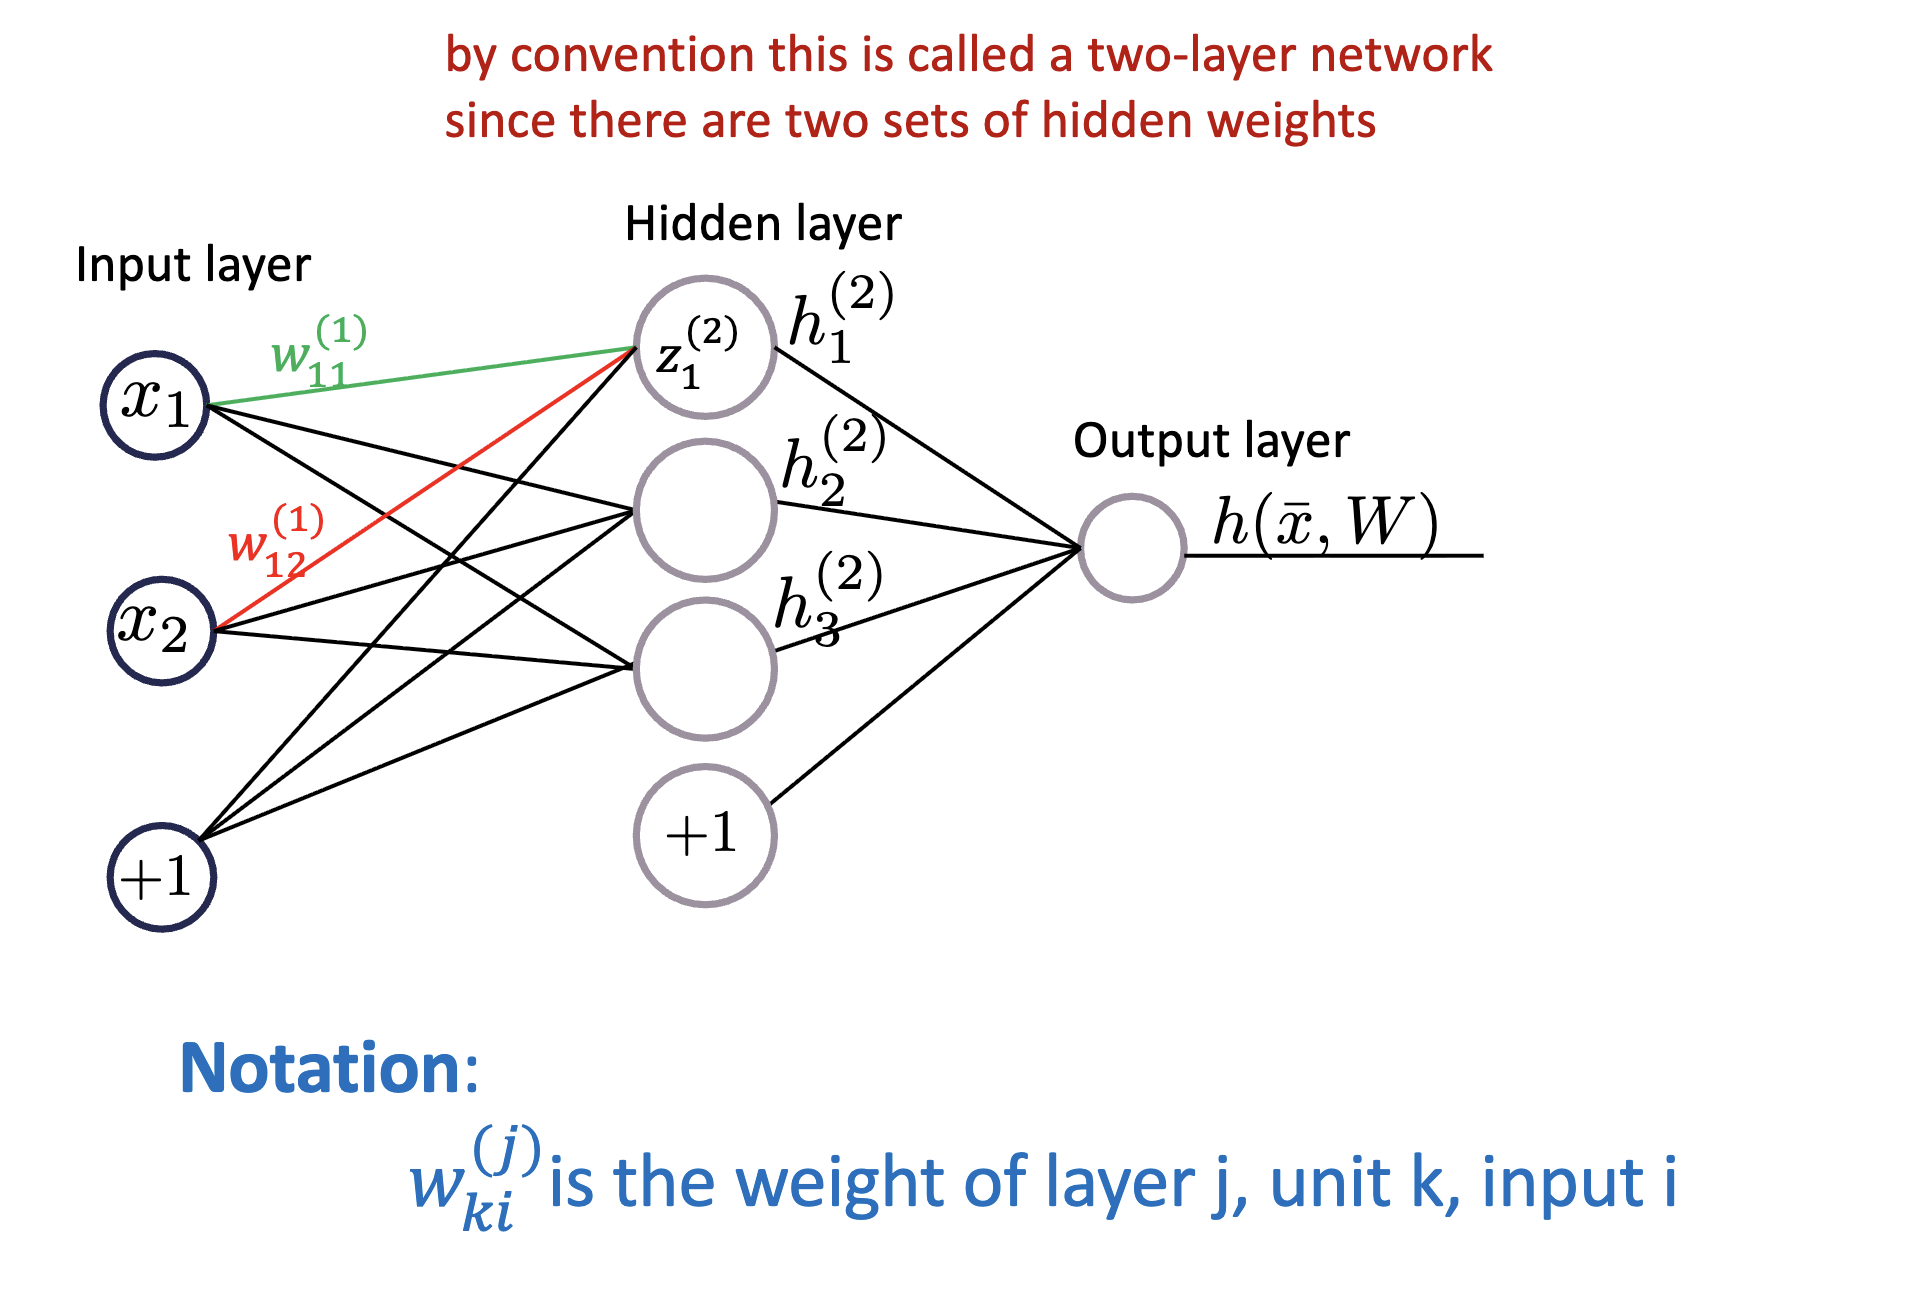
\includegraphics[width=0.75\linewidth]{images/two_layer_nn_example.png}

To get the inputs into the 2nd layer, we do the following:

\[ z_1^{(2)} = W_{11}^{(1)} x_1 + W_{12}^{(1)} x_2 + W_{10}^{(1)}, h_1^{(2)} = g(z_1^{(2)}) \]
\[ z_2^{(2)} = W_{21}^{(1)} x_1 + W_{22}^{(1)} x_2 + W_{20}^{(1)}, h_2^{(2)} = g(z_2^{(2)}) \]
\[ z_3^{(2)} = W_{31}^{(1)} x_1 + W_{32}^{(1)} x_2 + W_{30}^{(1)}, h_3^{(2)} = g(z_3^{(2)}) \]

For the output layer, we simply do same thing, propagated forward a layer:

\[ z^{(3)} = W_{11}^{(2)} h_1 + W_{12}^{(2)} h_2 + W_{13}^{(2)} h_3 + W_{10}^{(2)}, h(\bar x, W) = f(z^{(3)}) \]

\textbf{Note:} $f$ is potentially a different activation function from $g$. It is likely the Threshold function for classification. In fact, within a layer, neurons use the same activation function, and between layers, neurons use different activation functions.\\

This process of going layer by layer and (assumably) only using the most previous layer is called \textbf{forward propagation}

\section{Training Neural Networks}

Goal: Learn all weights for input neurons.\\
Idea: Use back-propagation, which is essentially SGD + chain rule.\\

Note: Remember, the number of hidden layers and the activation functions are all hyperparameters of the architecture. We will focus on non-hyperparameter selection for now.

\subsection{Single Layer NN}

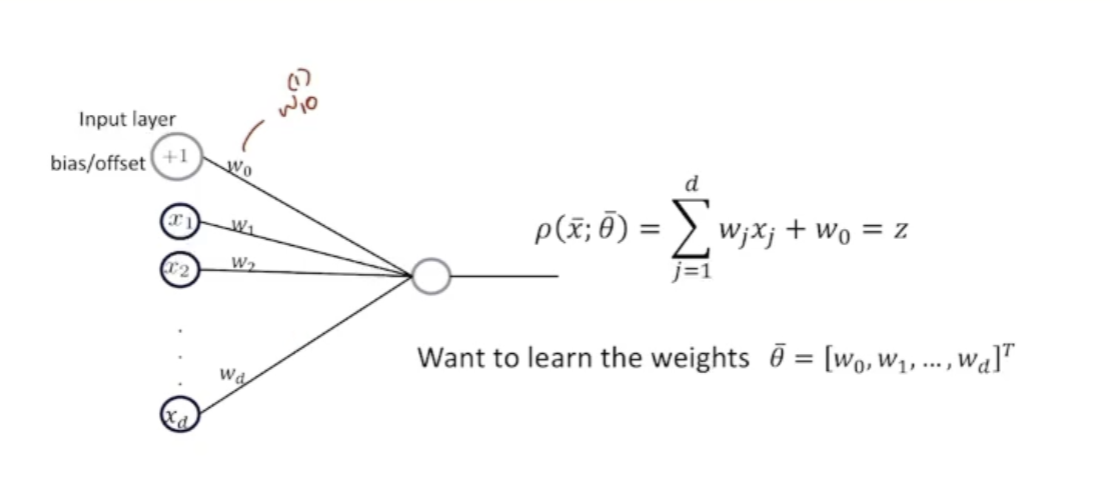
\includegraphics[width=0.75\linewidth]{images/training_nn_example.png}

Similar to earlier classification problems, we have the input dataset:

\[ S_n = \{ \bar{x}^{(i)}, y^{(i)} \}_{i=1}^n \qquad \bar x \in \R^d \qquad y \in \{ -1,1 \} \]

\textbf{Goal:} Learn model parameters $\bar{\theta}$ so as to minimize loss over the training examples

\[ J(\bar{\theta}) = \frac 1 n \sum_{i = 1}^n Loss\left( y^{(i)} z^{(i)}) \right) \]

\textbf{Idea:} sample a point at random, nudge parameters toward values that would improve classification on that particular example.\\

\textbf{Steps:}

\begin{enumerate}[label=(\alph*)]
	\item Initialize parameters to small random values
	\item Select a point $i$ at random
	\item Update the parameters based on the point and the gradient:
		\[ \bar{\theta}^{(k+1)} = \bar{\theta}^{(k)} - \eta_k \nabla_{\bar{\theta}} Loss(y^{(i)} z^{(i)}) \]
\end{enumerate}

\subsection{Calculating $\nabla_{\bar{\theta}} Loss(yz)$}

Assume we are using hinge loss, we need to find the following:

\[ \nabla_{\bar{\theta}} Loss(yz) = \nabla_{\bar{\theta}} max\{ 1-yz, 0 \} \]

So we need to find 

\[ \pdv{Loss(yz)}{w_j} = \pdv{Loss(yz)}{z} \pdv{z}{w_j} \quad \text{(chain rule)} \]

Since 

\[ z = \sum_{j=1}^d w_jx_j + w_0 \implies \pdv{z}{w_j} = x_j, \quad \text{and} \quad \pdv{Loss(yz)}{z} = 
	\begin{cases}
		-y & 1-yz > 0\\
		0 & \text{otherwise}
	\end{cases}
\]

We get

\[ 
	\pdv{Loss(yz)}{w_j} = 
	\begin{cases}
		-yx_j & 1-yz > 0\\
		0 & \text{otherwise}
	\end{cases}
\]

So our final updates to the individual weights in $\bar{\theta}$ are:

\[ w_j^{(k+1)} = w_j^{(k)} + \eta_k yx_j [[1 - yz > 0]] \]

\section{Two Layer NN with SGD}

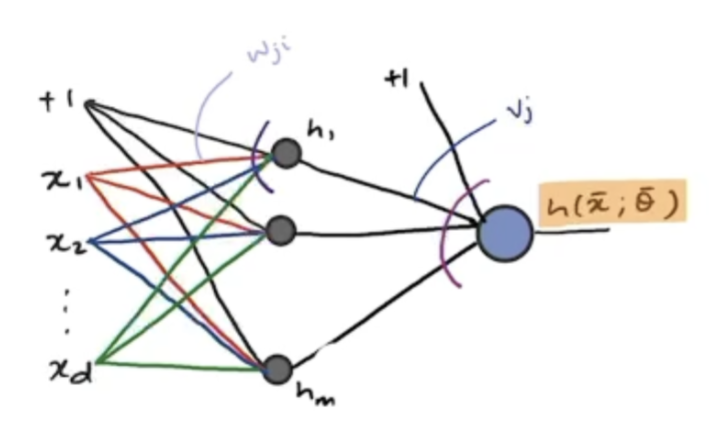
\includegraphics[width=0.75\linewidth]{images/two_layer_nn_with_diff_notation.png}

Since there are only two layers, for notational convenience, let's drop the superscript:\\

$w_{ji} = w_{ji}^{(1)}$ for $j= 1, \dots, m$, $i = 0, \dots, d$\\
$v_{j} = w_{ji}^{(2)}$ for $j= 0, \dots, m$\\
$z_{j} = z_{j}^{(2)}$ for $j= 1, \dots, m$\\
$h_{j} = h_{j}^{(2)}$ for $j= 1, \dots, m$\\
$z = z^{(3)}$\\

We are still be using hinge loss as our loss function and ReLU as our activation function.\\

So our non-weight values become:

\begin{equation}
	Loss(yz) = max\{ 1-yz, 0 \}, \quad z = \sum_{j=1}^m v_jh_j + v_0, \quad h_j = g(z_j) = max(0, z_j), \quad z_j = \sum_{i=1}^d w_{ji}x_i + w_{j0}
	\label{eq:two layer nn with sgd 1}
\end{equation}

\textbf{Goal:} Work out update for each parameter\\

\textbf{Last Layer Updates:}\\

Start with the last layer and work backwards. We loop through all the weights $w$ in the current layer and calculate the gradient of our loss function with respect to $w$. To do this, we will need to use the chain rule.\\

Referencing \ref{eq:two layer nn with sgd 1}, for each weight in the last layer, we get

\[ \pdv{Loss(yz)}{v_j} = \pdv{Loss(yz)}{z} \pdv{z}{v_j} = -yh_j[[(1-yz) > 0]] \]

So the update step becomes

\begin{equation}
	v_j^{(k+1)} = v_j^{(k)} + \eta_k yh_j[[(1-yz) > 0]]
	\label{eq:two layer nn with sgd 2}
\end{equation}

Notice that the last layer is a simple linear classifier, which makes sense because our last layer is a simple linear transformation layer.\\

\textbf{First Layer Updates:}\\

Update for parameters in the first layer is more complicated since we are computing the derivative of the composition of two or more functions.\\

\textbf{Idea: use back-propagation}\\
back-propagation = gradient descent + chain rule\\

Referencing \ref{eq:two layer nn with sgd 1}, for each weight in the first layer, we get

\begin{equation}
	\pdv{Loss(yz)}{w_{ji}} = \pdv{Loss(yz)}{z} \pdv{z}{h_j} \pdv{h_j}{z_j} \pdv{z_j}{w_{ji}} = -y[[1-yz > 0]] v_j [[z_j > 0]] x_i	\label{eq:two layer nn with sgd 3}
\end{equation}

So the update step becomes

\begin{equation}
	w_{ji}^{k+1} = w_{ji}^{(k)} + \eta_k y[[1-yz > 0]] v_j [[z_j > 0]] x_i
	\label{eq:two layer nn with sgd 4}
\end{equation}

\part{Lecture 12}

\subsection{Overall Algorithm}

\textbf{Idea:} sample a point at random, nudge parameters toward values that would improve classification on that particular example\\

\textbf{Steps:}

\begin{enumerate}
	\item Initialize parameters $\bar{\theta}$ to small random values
	\item For each training instance $\{ \bar x^{(i)}, y^{(i)} \}$
		\begin{enumerate}
			\item Make a prediction $\rho(\bar x^{(i)}, \bar{\theta})$, called forward propagation
			\item Measure the loss of the prediction $\rho(\bar x^{(i)}, \bar{\theta}) = z^{(i)}$ with respect to the true label $y^{(i)}$ 
				\[ Loss(y^{(i)} z^{(i)} \]
			\item Go through each layer in reverse to measure the error contribution of each connection, called back-propagation. 
			\item Tweak weight to reduce error (SGD update step)
				\[ \bar{\theta}^{(k+1)} = \bar{\theta}^{(k)} - \eta_k \nabla_{\bar{\theta}} Loss(y^{(i)} z^{(i)}) \]
				Where $\nabla_{\bar{\theta}} Loss(y^{(i)} z^{(i)})$ is computed using eq \ref{eq:two layer nn with sgd 2} and eq \ref{eq:two layer nn with sgd 3}
		\end{enumerate}
\end{enumerate}

One thing to note about NN is that unlike with linear models, the loss functions in NN are not convex, meaning that locations with a zero gradient are not necessarily global minimums but instead could be local minimums. Thus, we could end up training a model that gets stuck in one of these local minimums, which is why initializing parameters $\bar{\theta}$ at the beginning of the algorithm becomes essential to learning an efficient model. To get out of a local minimum, we can rerun the algorithm with different initial weights and hope it ends up at a lower minimum.

\subsection{Pros and Cons}

\textbf{Pros:} Universal Approximation Theorem (UAT) - A feedforward neural network with a single hidden layer can approximate any continuous function on compact subsets of $\R^n$ to arbitrary percision, given a non-polynomial activation function. In other words, any reasonable classification problem can be solved using a 2-layer NN.\\

\textbf{Cons:} Since you can learn pretty much any function with NN, you can very overfit to training datasets. In other words, you can very easily learn noise as well.

\section{NNs: Details}

\begin{itemize}
	\item How to choose an architecture
	\item Avoiding Overfitting
	\item How to pick learning rate
	\item Issues with gradient values
\end{itemize}

\subsection{NN: Number of hidden layers}

\begin{itemize}
	\item NN with one hidden layer can model complex functions provided it has enough neurons (i.e., is wide)
		\begin{itemize}
			\item In fact, 2 layer NNs can approximate any function (UAT)
		\end{itemize}
	\item Deeper nets can converge faster to a good solution
	\item Take-away: Start with 1-2 hidden layers and ramp up until you start to overfit
\end{itemize}

\subsection{NN: Number of Neurons per Hidden Layer}

\textbf{Number of Neurons per Hidden layer}
\begin{itemize}
	\item \# nodes in input \& output determined by task at hand
	\item Common practice: same size for all hidden layers so that you only have one tuning parameter across all layers
	\item Take-away: Increase number of neurons until you start to overfit
\end{itemize}

\subsection{NN: How to set learning rate}

\begin{itemize}
	\item \textbf{Simple recipe:} Keep it fixed and use the same for all parameters.
		\begin{itemize}
			\item \textbf{Note:} better results can generally be obtained by allowing learning rates to decrease (learning schedule)
		\end{itemize}
\end{itemize}

\subsection{NN: Reducing Overfitting}
 
\begin{enumerate}
	\item Early stopping: interrupt training when performance on the validation set starts to decrease
	\item L1 \& L2 regularization: applied as before to all weights
	\item Dropout\\
		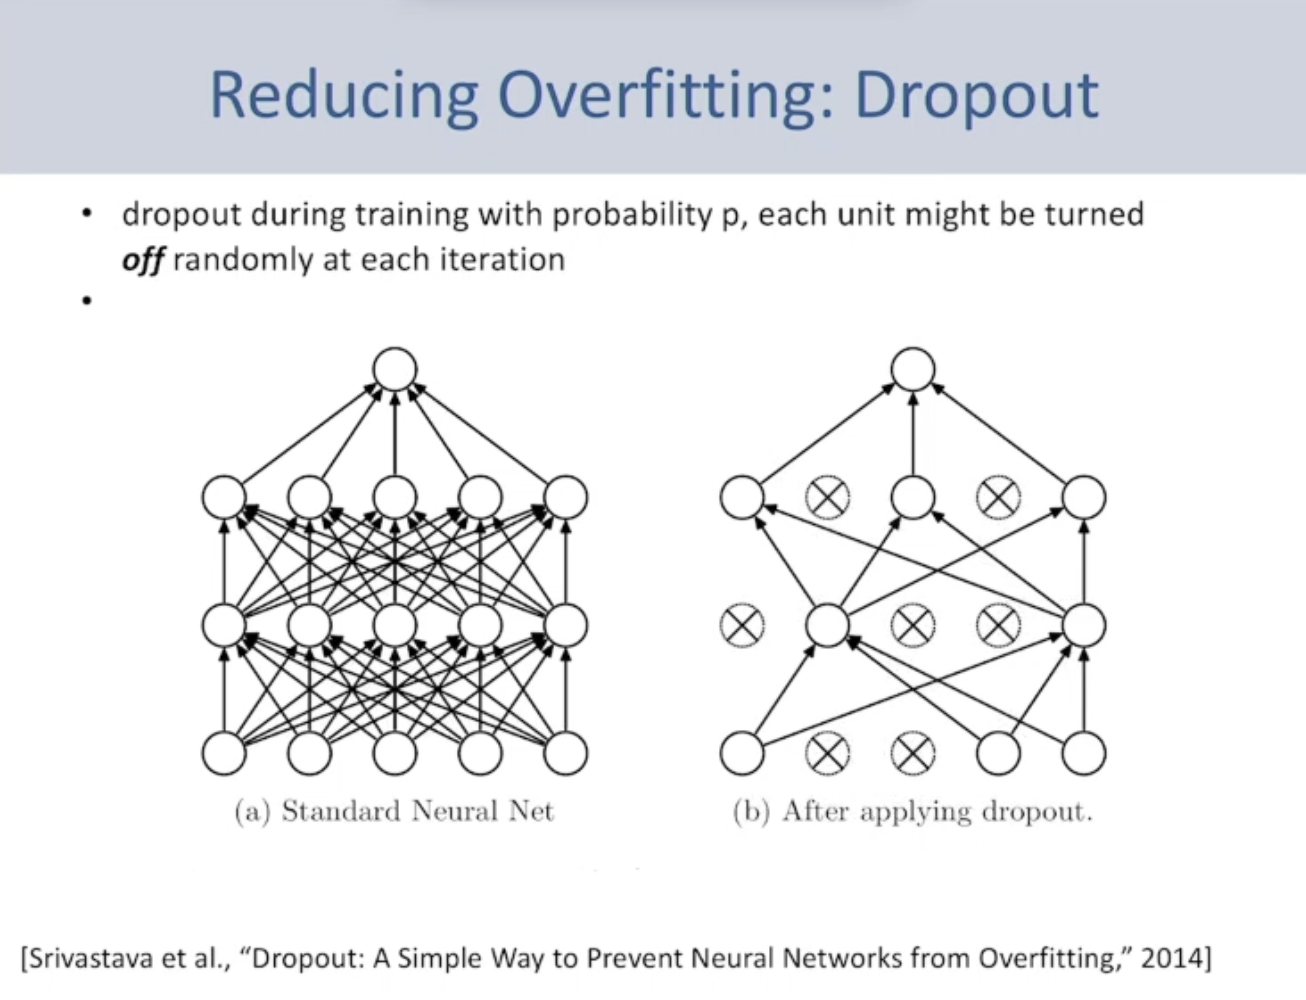
\includegraphics[width=0.75\linewidth]{images/dropout.png}
\end{enumerate}

\subsection{Vanishing/Exploding Gradient}

\begin{itemize}
	\item It turns out that the gradient in deep neural networks is unstable, tending to either exploding or vanishing in earlier layers.
		\begin{itemize}
			\item e.g., sometimes gradients get smaller and smaller as the algorithm progresses down to the lower layers, this can leave the lower layer connection weights virtually unchange and training never converges to a good solution.
			\item solutions include gradient clipping, non-saturationg activation function (dying ReLU) and proper weight initialization.
		\end{itemize}
\end{itemize}

\part{Lecture 13}

\section{Convolutional Neural Networks}

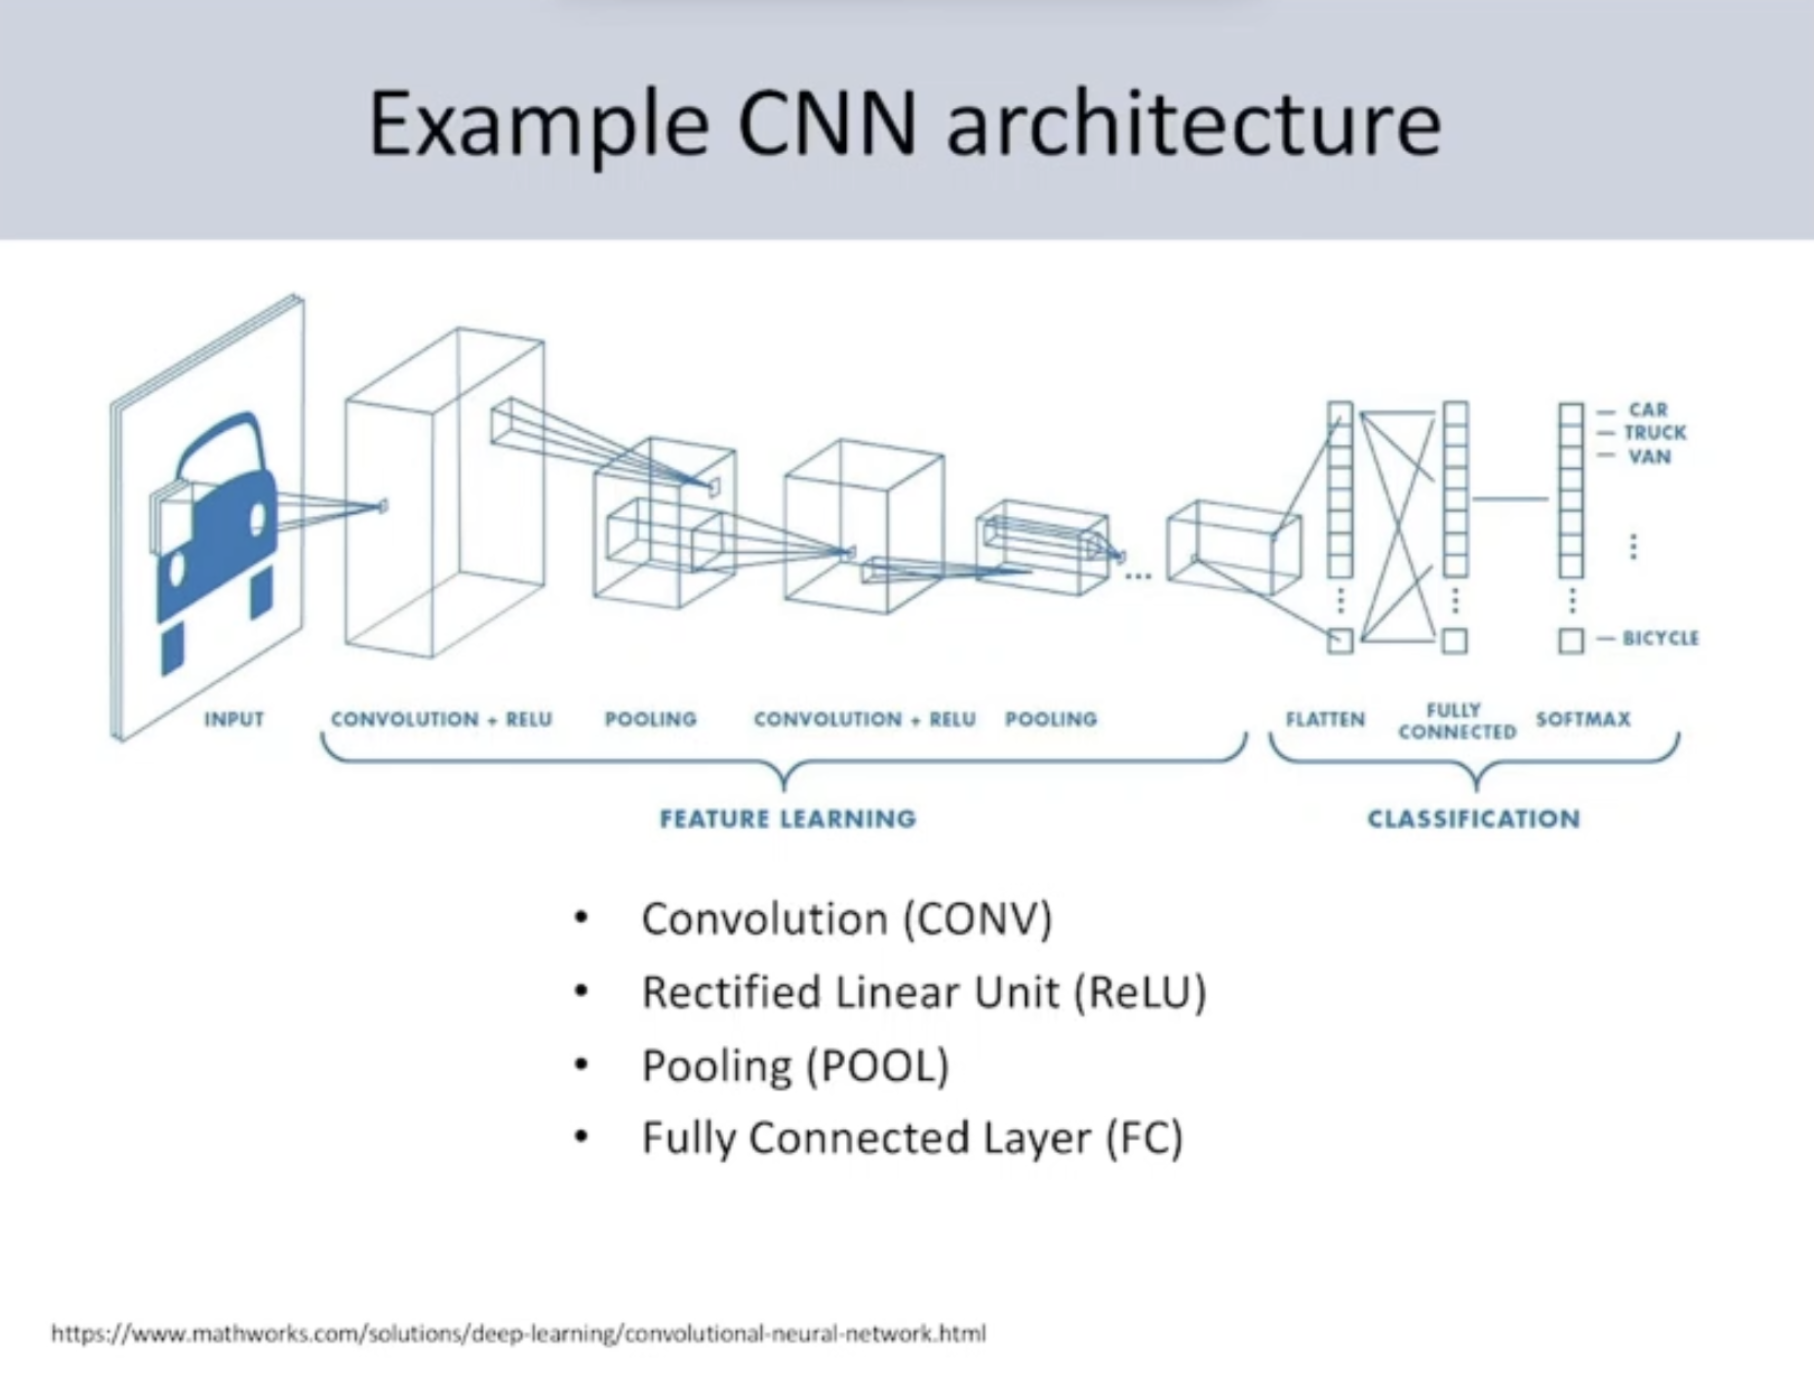
\includegraphics[width=0.75\linewidth]{images/cnn_example_1.png}

\begin{itemize}
	\item Class of neural networks used primarily in computer vision
		\begin{itemize}
			\item image recognition and classification
			\item identifying faces, objects and traffic signs
		\end{itemize}
\end{itemize}

One observation about pictures is that pixels that are close to one another have higher relationship that pixels that are further apart. CNNs try to exploit this tendancy.\\

\textbf{Question:} Given that the universal approximation theorem exists, what is the point of using CNNs? Aren't they simply added complexity?\\

\textbf{Answer:} When we look at pictures, the proximity of pixels to one another conveys meaning. CNNs encode this information into the neural network and pushes it towards using this fact. Normal NNs would need many more parameters and configurations to learn these patterns by themselves, leading to more complexity and larger input sizes. For example, when we try to classify the picture below, the O and the P must be next to each other for it to be a stop sign. A CNN has this tendancy of grouping pixels together already encoded into its design, leading to less number of parameters and faster conversion time.

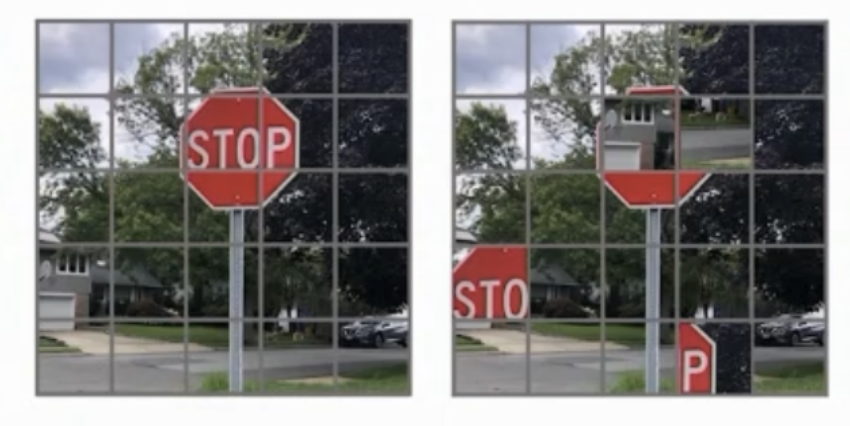
\includegraphics[width=0.75\linewidth]{images/cnn_example_2.png}



\subsection{Convolutional Layer}

One of the layers of the CNN is called the convolution layer.\\

\textbf{Steps:}
\begin{enumerate}
	\item Decide on the dimensions and stepsize of the filter. This is dependent on the architecture (hyperparameters)
	\item Learn the values/weights in the filter
	\item convolve the filter over the input image\\
		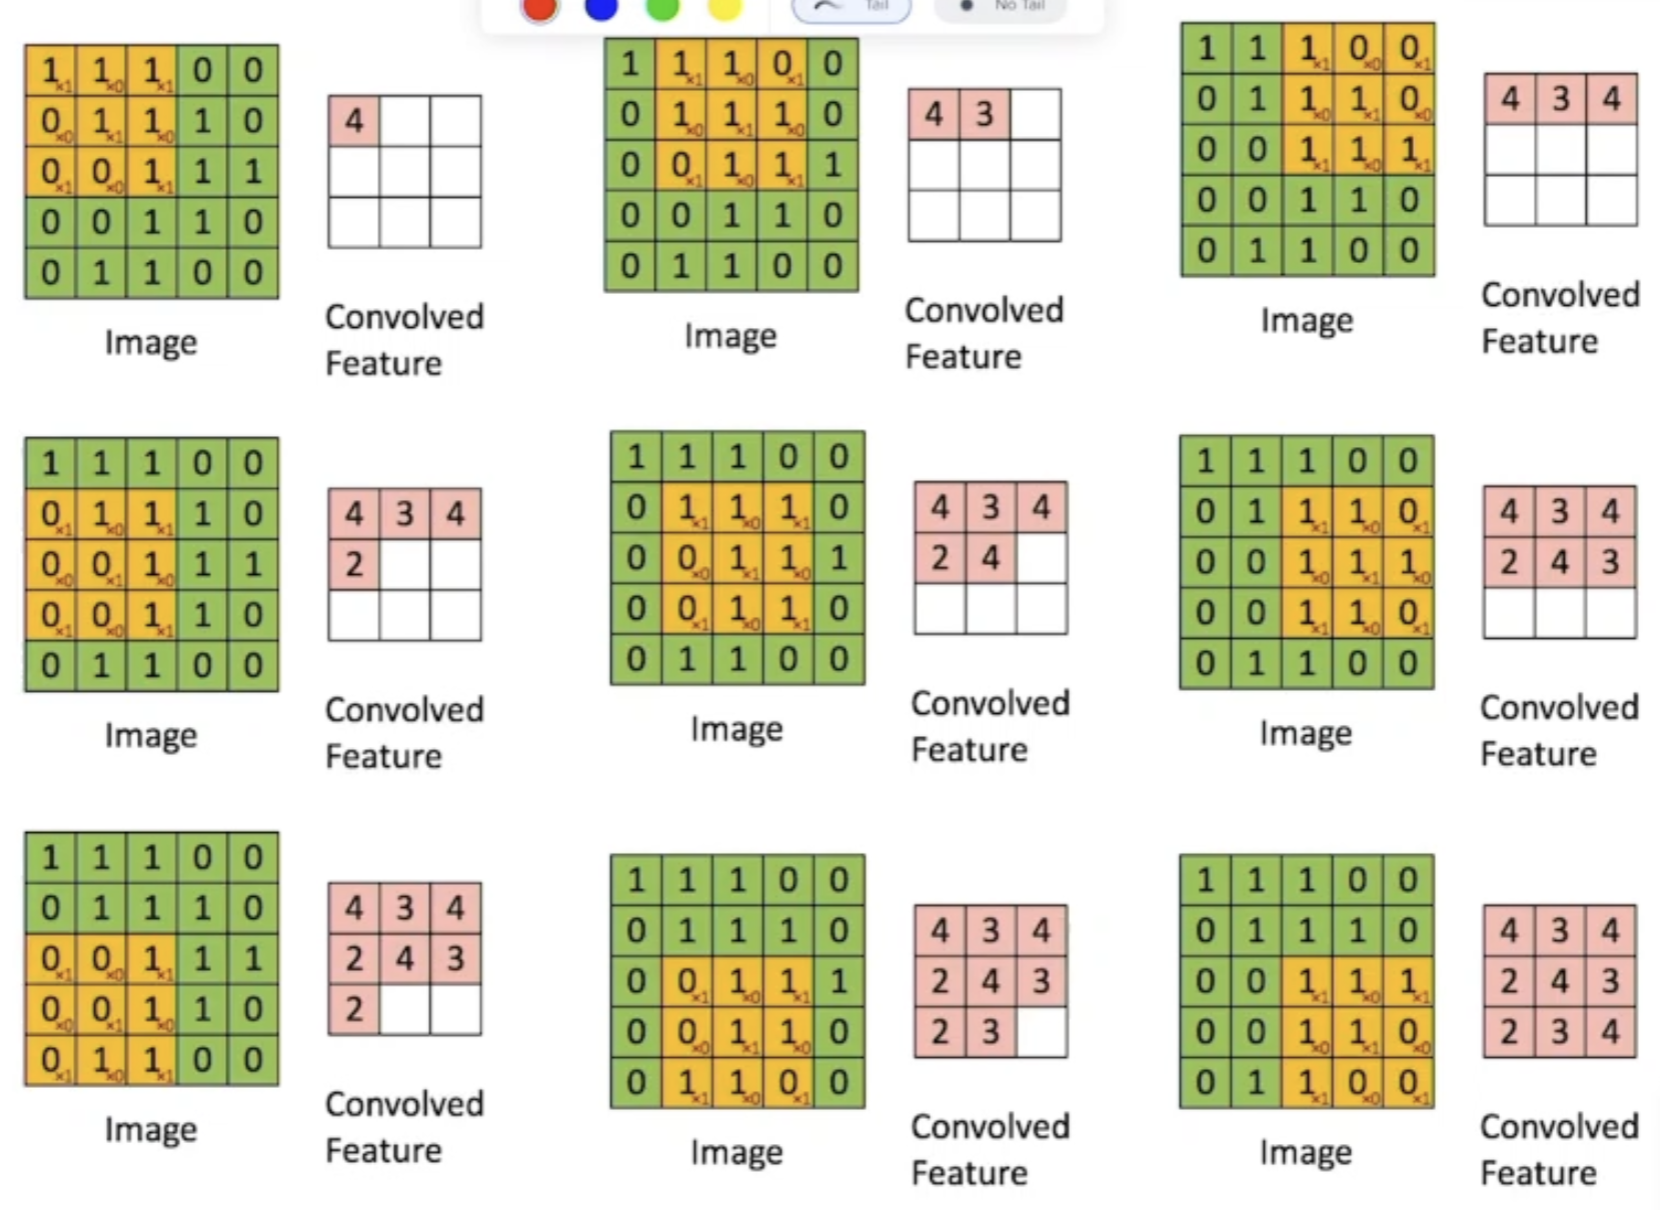
\includegraphics[width=0.75\linewidth]{images/convolve_example_1.png}
\end{enumerate}

You can think of a filter as simply taking the dot product of two flattened vectors. You flatten a subsection of the input and dot it with the flattened version of your filter. The dimesions of your filter will determine how the input gets flattened. Filters can be any dimensional. If you have an image input, then the input will be 3 dimensional (height, width, and RGB). The corresponding filter could be 3 dimensional. 

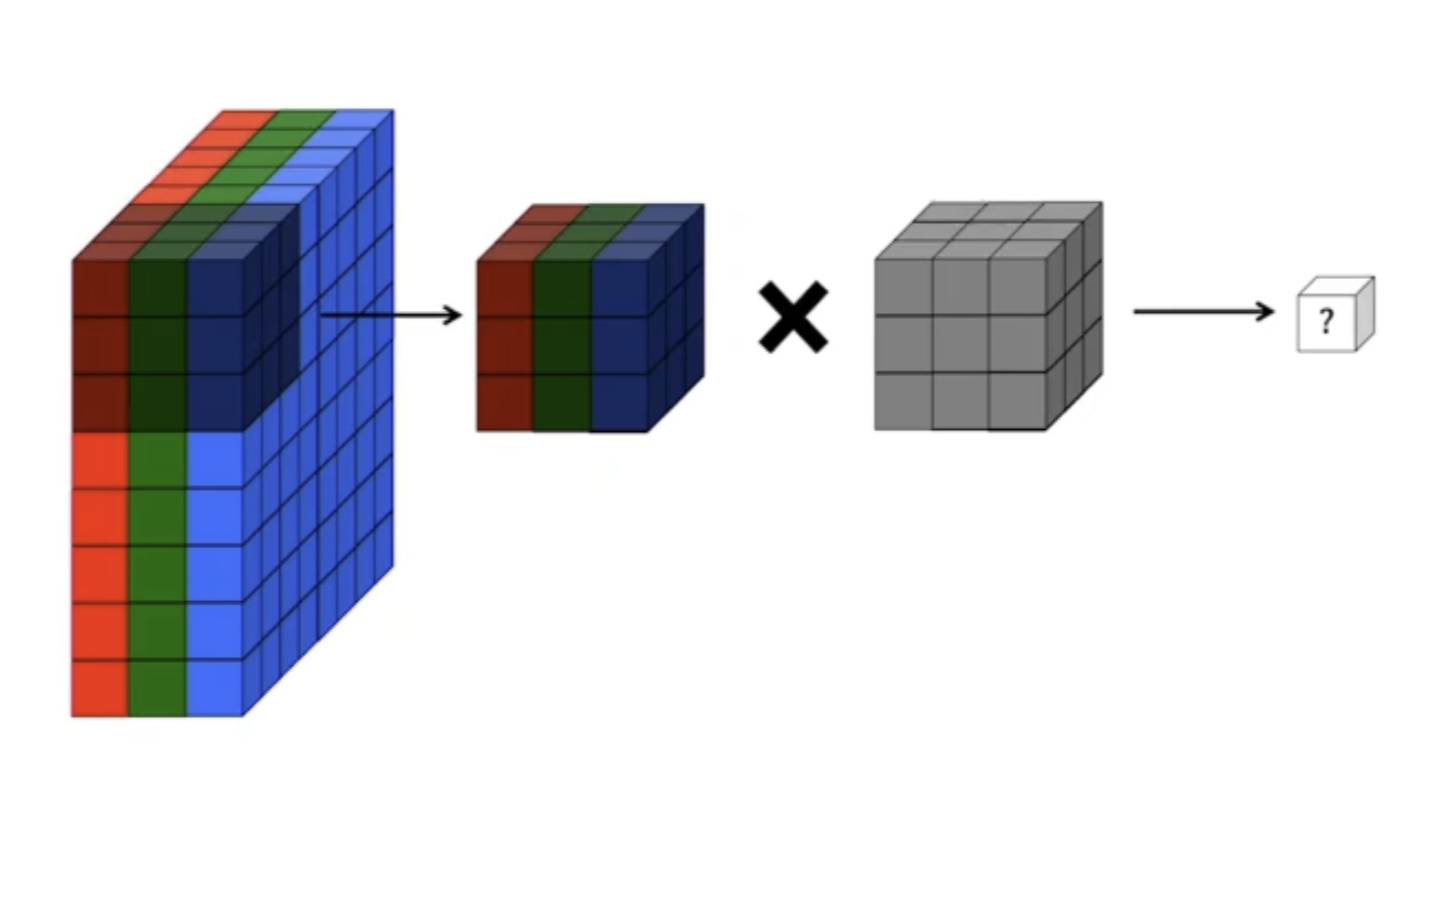
\includegraphics[width=0.75\linewidth]{images/convolve_example_2.png}

Additionally, a convolution layer can have several ($> 1$) filters. The result after convolving the image with these filters will have an additional dimension equal to the number of filters used.\\

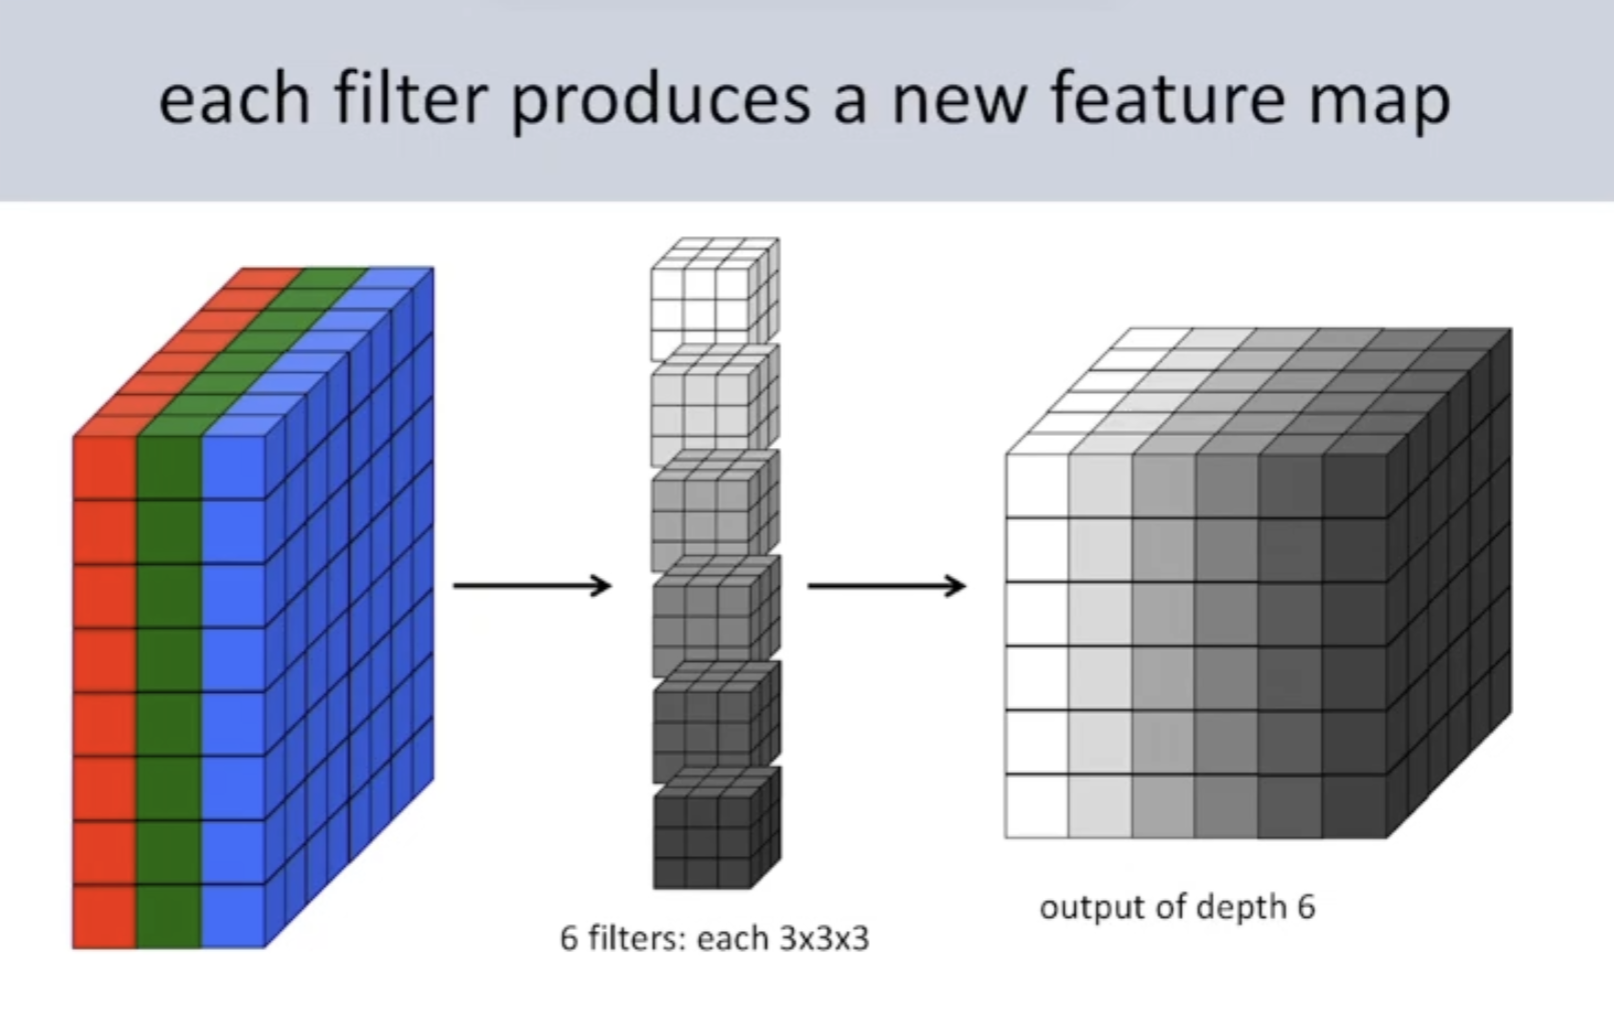
\includegraphics[width=0.75\linewidth]{images/convolve_example_3.png}

\subsection{Filter details}

\begin{itemize}
	\item Each filter produces a new feature map.
		\begin{itemize}
			\item Intuitively, network learns filters that activate on details in intial layers and more "holistic" features on later layers
				\begin{itemize}
					\item e.g., on first layer edge detection and higher layers wheel-like patterns
				\end{itemize}
		\end{itemize}
	\item Hyperparameters:
		\begin{itemize}
			\item number of filters
			\item stride length (how much a filter moves between iterations)
			\item filter size (dimensions)
			\item zero-padding (reference zero-padding picture). Besides preserving the size of the original input, zero-padding also results in the edge cells being less under-represented than before.
		\end{itemize}
	\item Efficiency concerns
		\begin{itemize}
			\item parameter sharing (same weights across all depths)
		\end{itemize}
\end{itemize}

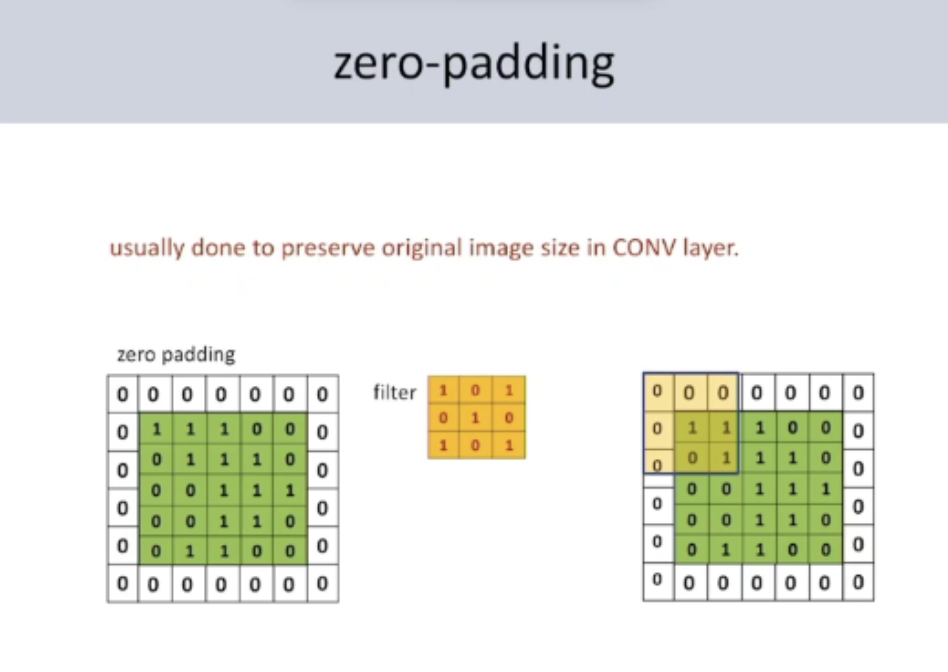
\includegraphics[width=0.75\linewidth]{images/convolve_example_4.png}

\subsection{ReLU Layer}

Apply ReLU to each cell in the input (the input could be the output of the convolution layer)\\

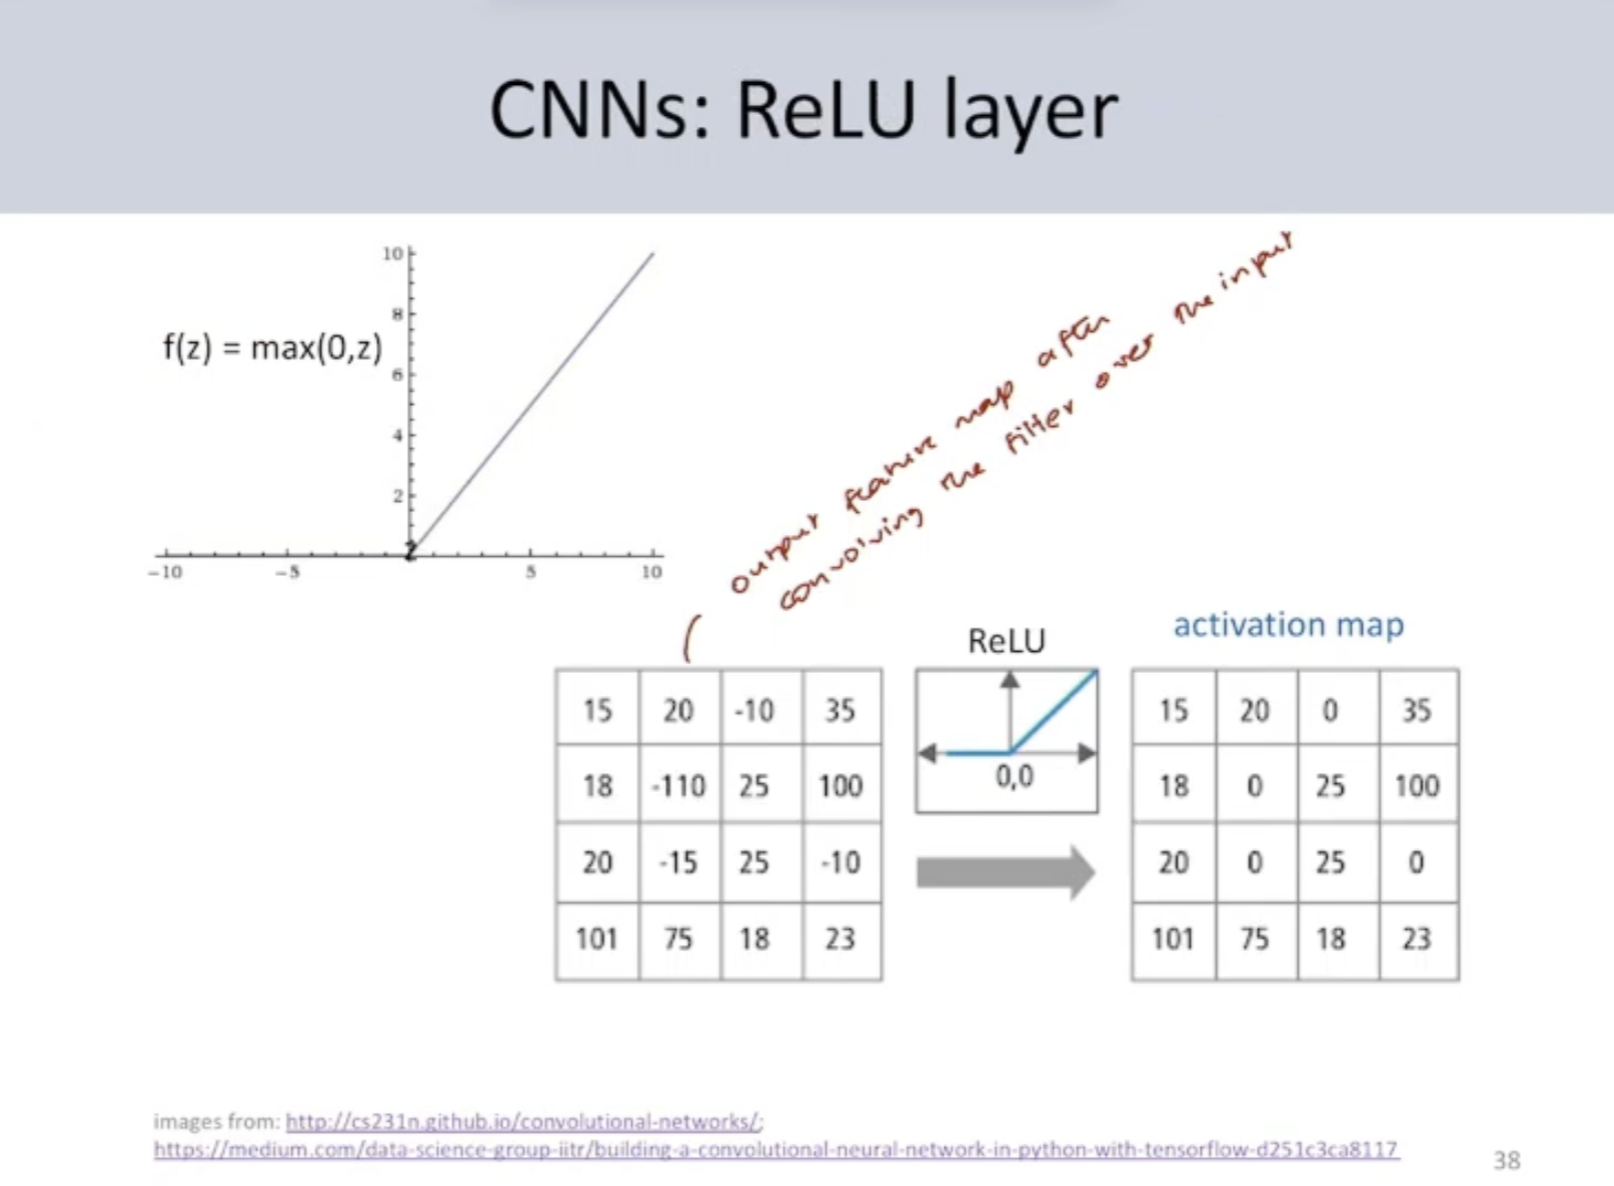
\includegraphics[width=0.75\linewidth]{images/cnn_relu_layer_example_1.png}

\subsection{Pooling Layer}

\textbf{Idea:} reduce dimensionality of feature map/compress input while retaining significant information. As a consequence, control overfitting. One possible pooling technique is \textbf{max pooling}, where, similar to the convolution layer, you have a filter and take the max of the cells in the filter.\\

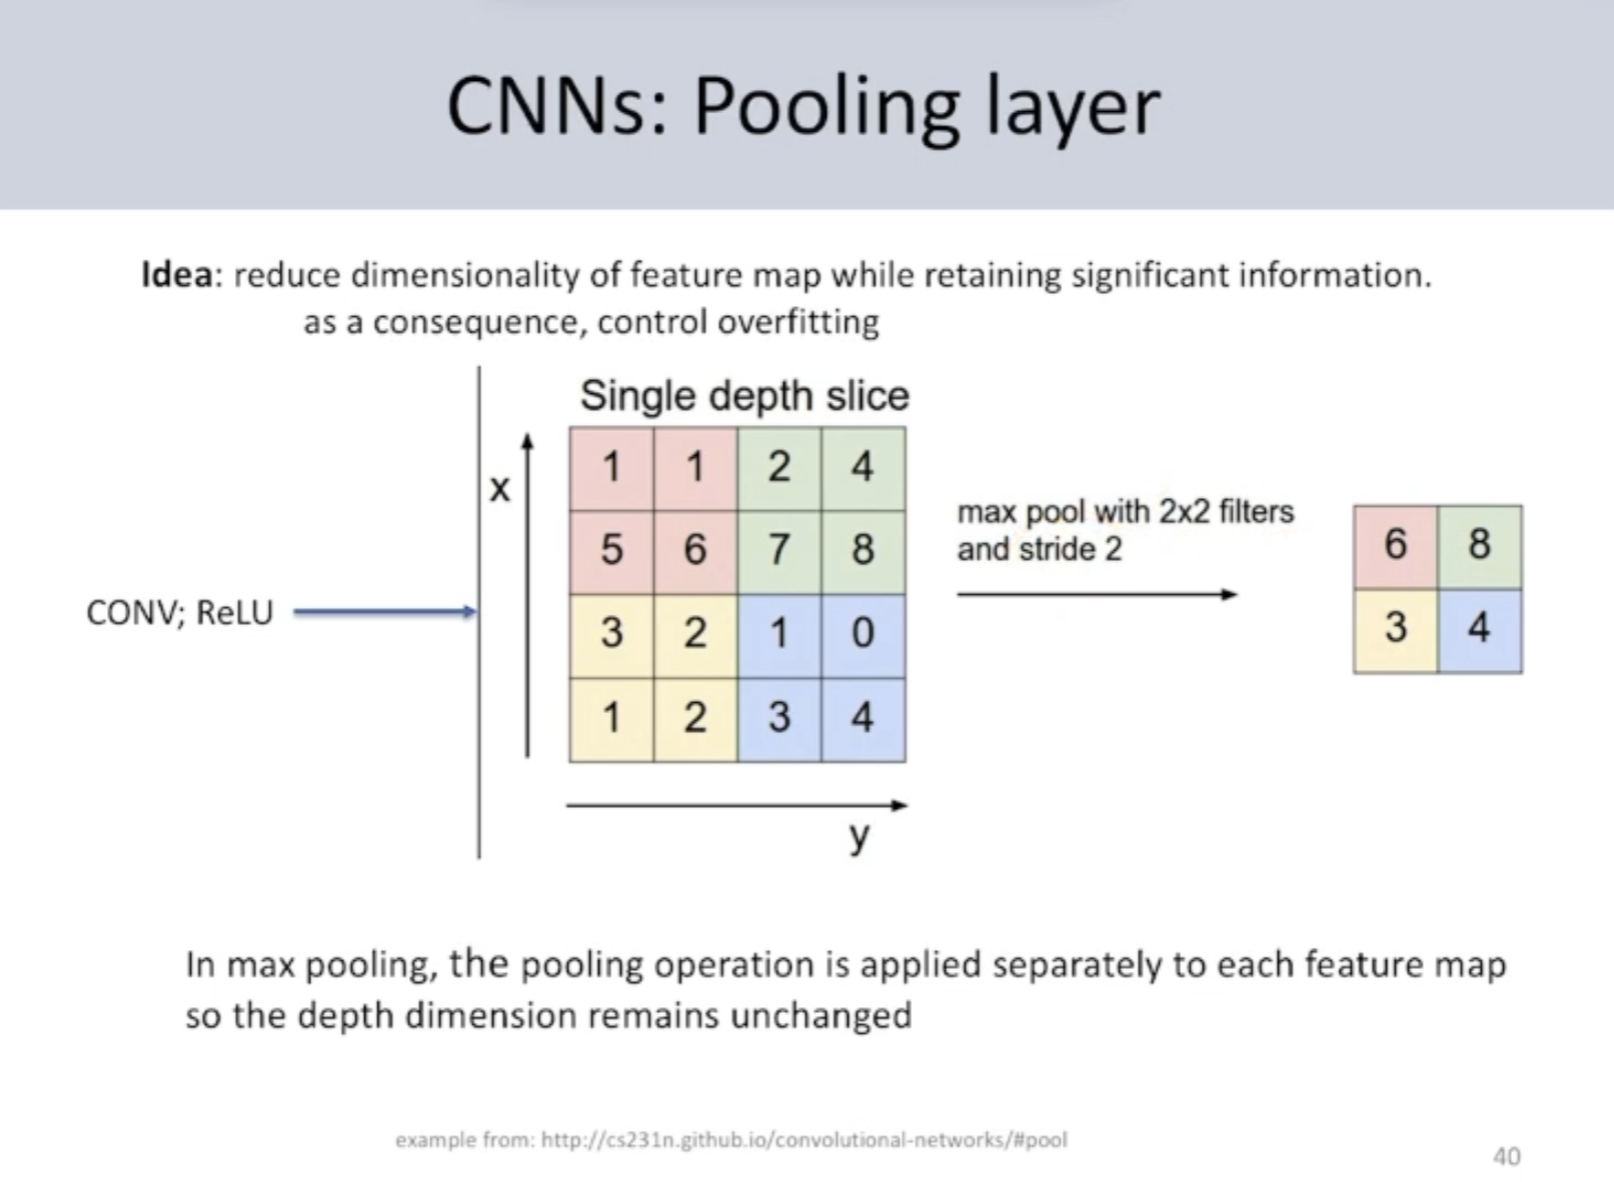
\includegraphics[width=0.75\linewidth]{images/cnn_pool_layer_example_1.png}\\

Max pooling leaves depth unchanced, so you end up with somehting like this:

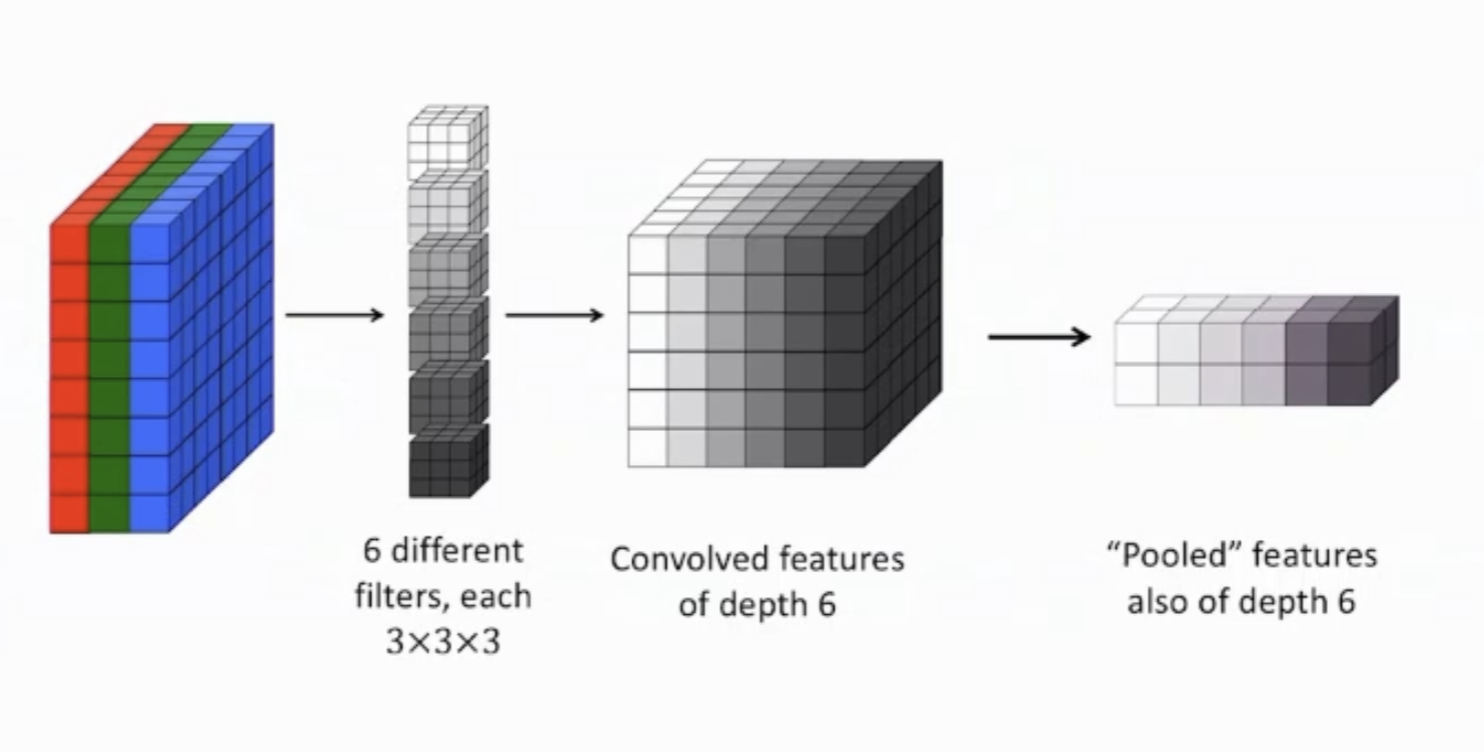
\includegraphics[width=0.75\linewidth]{images/cnn_pool_layer_example_2.png}

\subsection{Fully Connected Layer}

This is the NN algorithm that we talked about before CNNs. Take the output from the previous layers, flatten it, and that will be the input to the learned NN. 

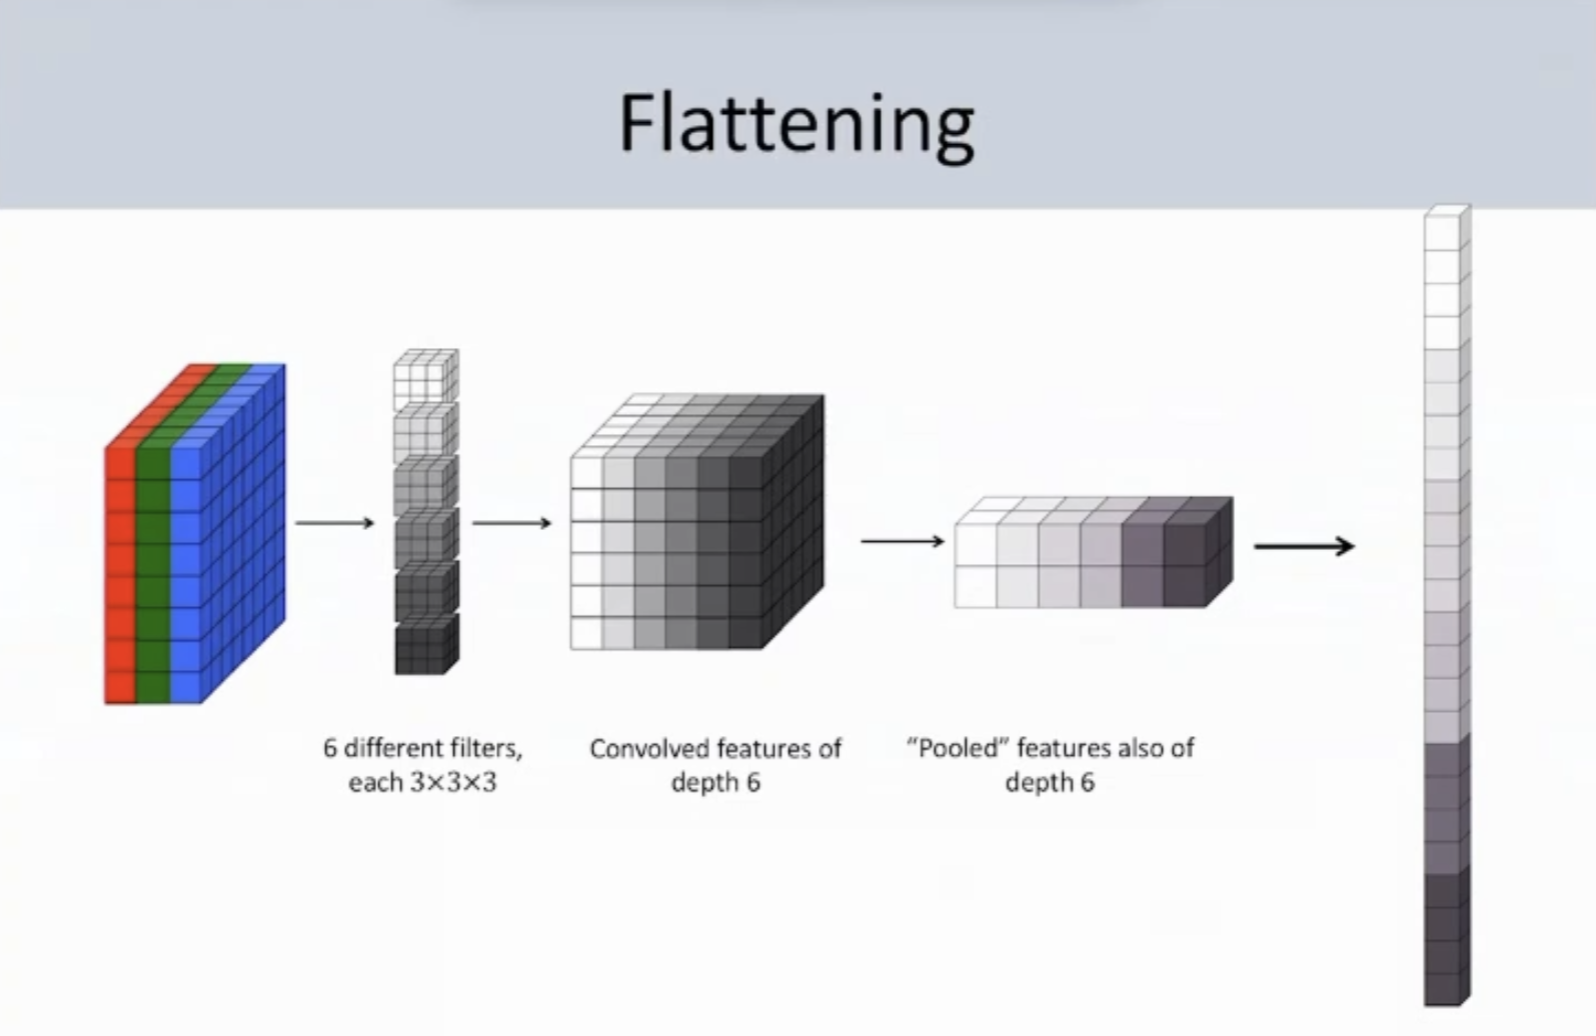
\includegraphics[width=0.75\linewidth]{images/cnn_flattening_example_1.png}

\subsection{Softmax neurons}

Oftentimes, each output neuron for our fully connected NN will give a probability for how likely the input image should be classified as a certain class, giving us a total of (\# of unique classes) output neurons. To transform this information into a prediction, we usually use the softmax function and take the max of the results. The softmax function is defined as:

\[ \hat{y}_j = \frac{e^{z_j}}{\sum_k e^{z_k}} \]

Essentially, this gives us another layer of neurons that takes in the output neurons $\bar{z}$ as inputs. We call this layer of neurons the softmax neurons, and they have a couple of really nice properties:

\begin{itemize}
	\item They gives real-valued output that is a smooth and bounded function of their total input
		\begin{itemize}
			\item The outputs sum up to 1 (useful for classification problems)
			\item They have nice derivatives which makes analysic easier
		\end{itemize}
\end{itemize}

Once you have the output of this softmax layer, you want to compute the loss. Obviously, a softmax layer that has an output that has the actual class predicted much higher than the other classes is preferred. So we cross entropy loss:

\[ Loss(\bar y, \hat y) = -\sum_j \bar y_j \log \hat y_j\]

\textbf{Note:} $\bar y \in R^{(\text{\# of classes})}$ is a vector of all 0s for all classes $\ne$ true class, and 1 for the class $=$ true class. 

\subsection{Overview: Training a CNN}

\begin{itemize}
	\item Initialize parameters (weights, filter values, etc)
	\item Forware propagate a training example (image)
		\begin{itemize}
			\item i.e., through convolution, ReLU, pooling and fully connected layers
			\item compute class probabilities
		\end{itemize}
	\item Calculated the loss at the output layer
	\item Use backprop to calculate error contribution of each layer (how do you backprop through the convolution, ReLU and pooling layer?)
	\item update parameter values to minimize the output error
\end{itemize}

\newpage

\part{Lecture 14}

\section{Transfer Learning}

We have already talked about a couple of ways to reduce biases in our models (regularization and dropout). Transfer Learning is another way to reduce this bias and tries to solve a unique case of bias.\\

\textbf{Idea:} Some problems (target task) have a very small sample set of data that you want to learn features from. This makes the models that are generated from these datasets very prone to high bias. However, if you think there is another problem (source task) that has some similar features to the target task and much more data to train on, you can train some of your model on the source task to try to reduce this bias.

\begin{itemize}
	\item Addresses the challenge of small dataset. 
	\item Have:
		\begin{itemize}
			\item Data from target task: $S_n = \{ (\bar x^{(i)}, y^{(i)}) \}_{i=1}^n$
			\item Data from a related source task: $S'_m = \{ (\bar x^{(i)}, y^{(i)}) \}_{i=1}^m$
			\item Typically: source and target inputs lie in the same space and $m >> n$
		\end{itemize}
	\item Intuition: Patterns learned in the source task can help with the target class
\end{itemize}

\subsection{Transfer Learning: Main Application}

Recall that different features of a picture are learned at different layers of a CNN Lower-level features, like edge detection, can be shared across tasks.\\

\textbf{Step 1:} Pre-training - Using source task as training dataset to train a NN (learning all the weights).\\

\textbf{Step 2:} Adjust model to target task. There are two main ways of doing this to be aware of:

\begin{enumerate}
	\item Linear Probing: Fix all the weights of your model except for the last layer weights. Thus, you are really only changing the linear combination of the final layer of neurons, which is why it is called linear probing. 
	\item Fine-tuning: Use the trained weights from the source task as initialized weights and normally traing the NN as usual (keeping none of the weights fixed). This is better than just regularly training the NN on the target dataset since the loss function of a NN is not convex, making initialization of weights important.
\end{enumerate}

You can also do Transfer Learning using a combination of Linear Probing and Fine-tuning by choosing $k$ layers to freeze and training the remaining $L-k$ layers. 

\section{Data Augmentation}

Another way to combat the "too small dataset" problem is through data augmentation. The idea is that you can augment your data a little, like flipping or rotating an image, and the model should still be able to pick up the features and classify the image correctly under these augmentations. As a result, you get more datapoints to train your NN on.

\section{Recurrent Neural Network (RNN)}

\subsection{Sequence Model}

Many problems in ML involve sequences. Some examples are languange translation, where the input is a sequence of words and the output is another sequence of words. You can visualize what an ML architecture would look like and how they would differ from previous tasks for these sorts of problems.

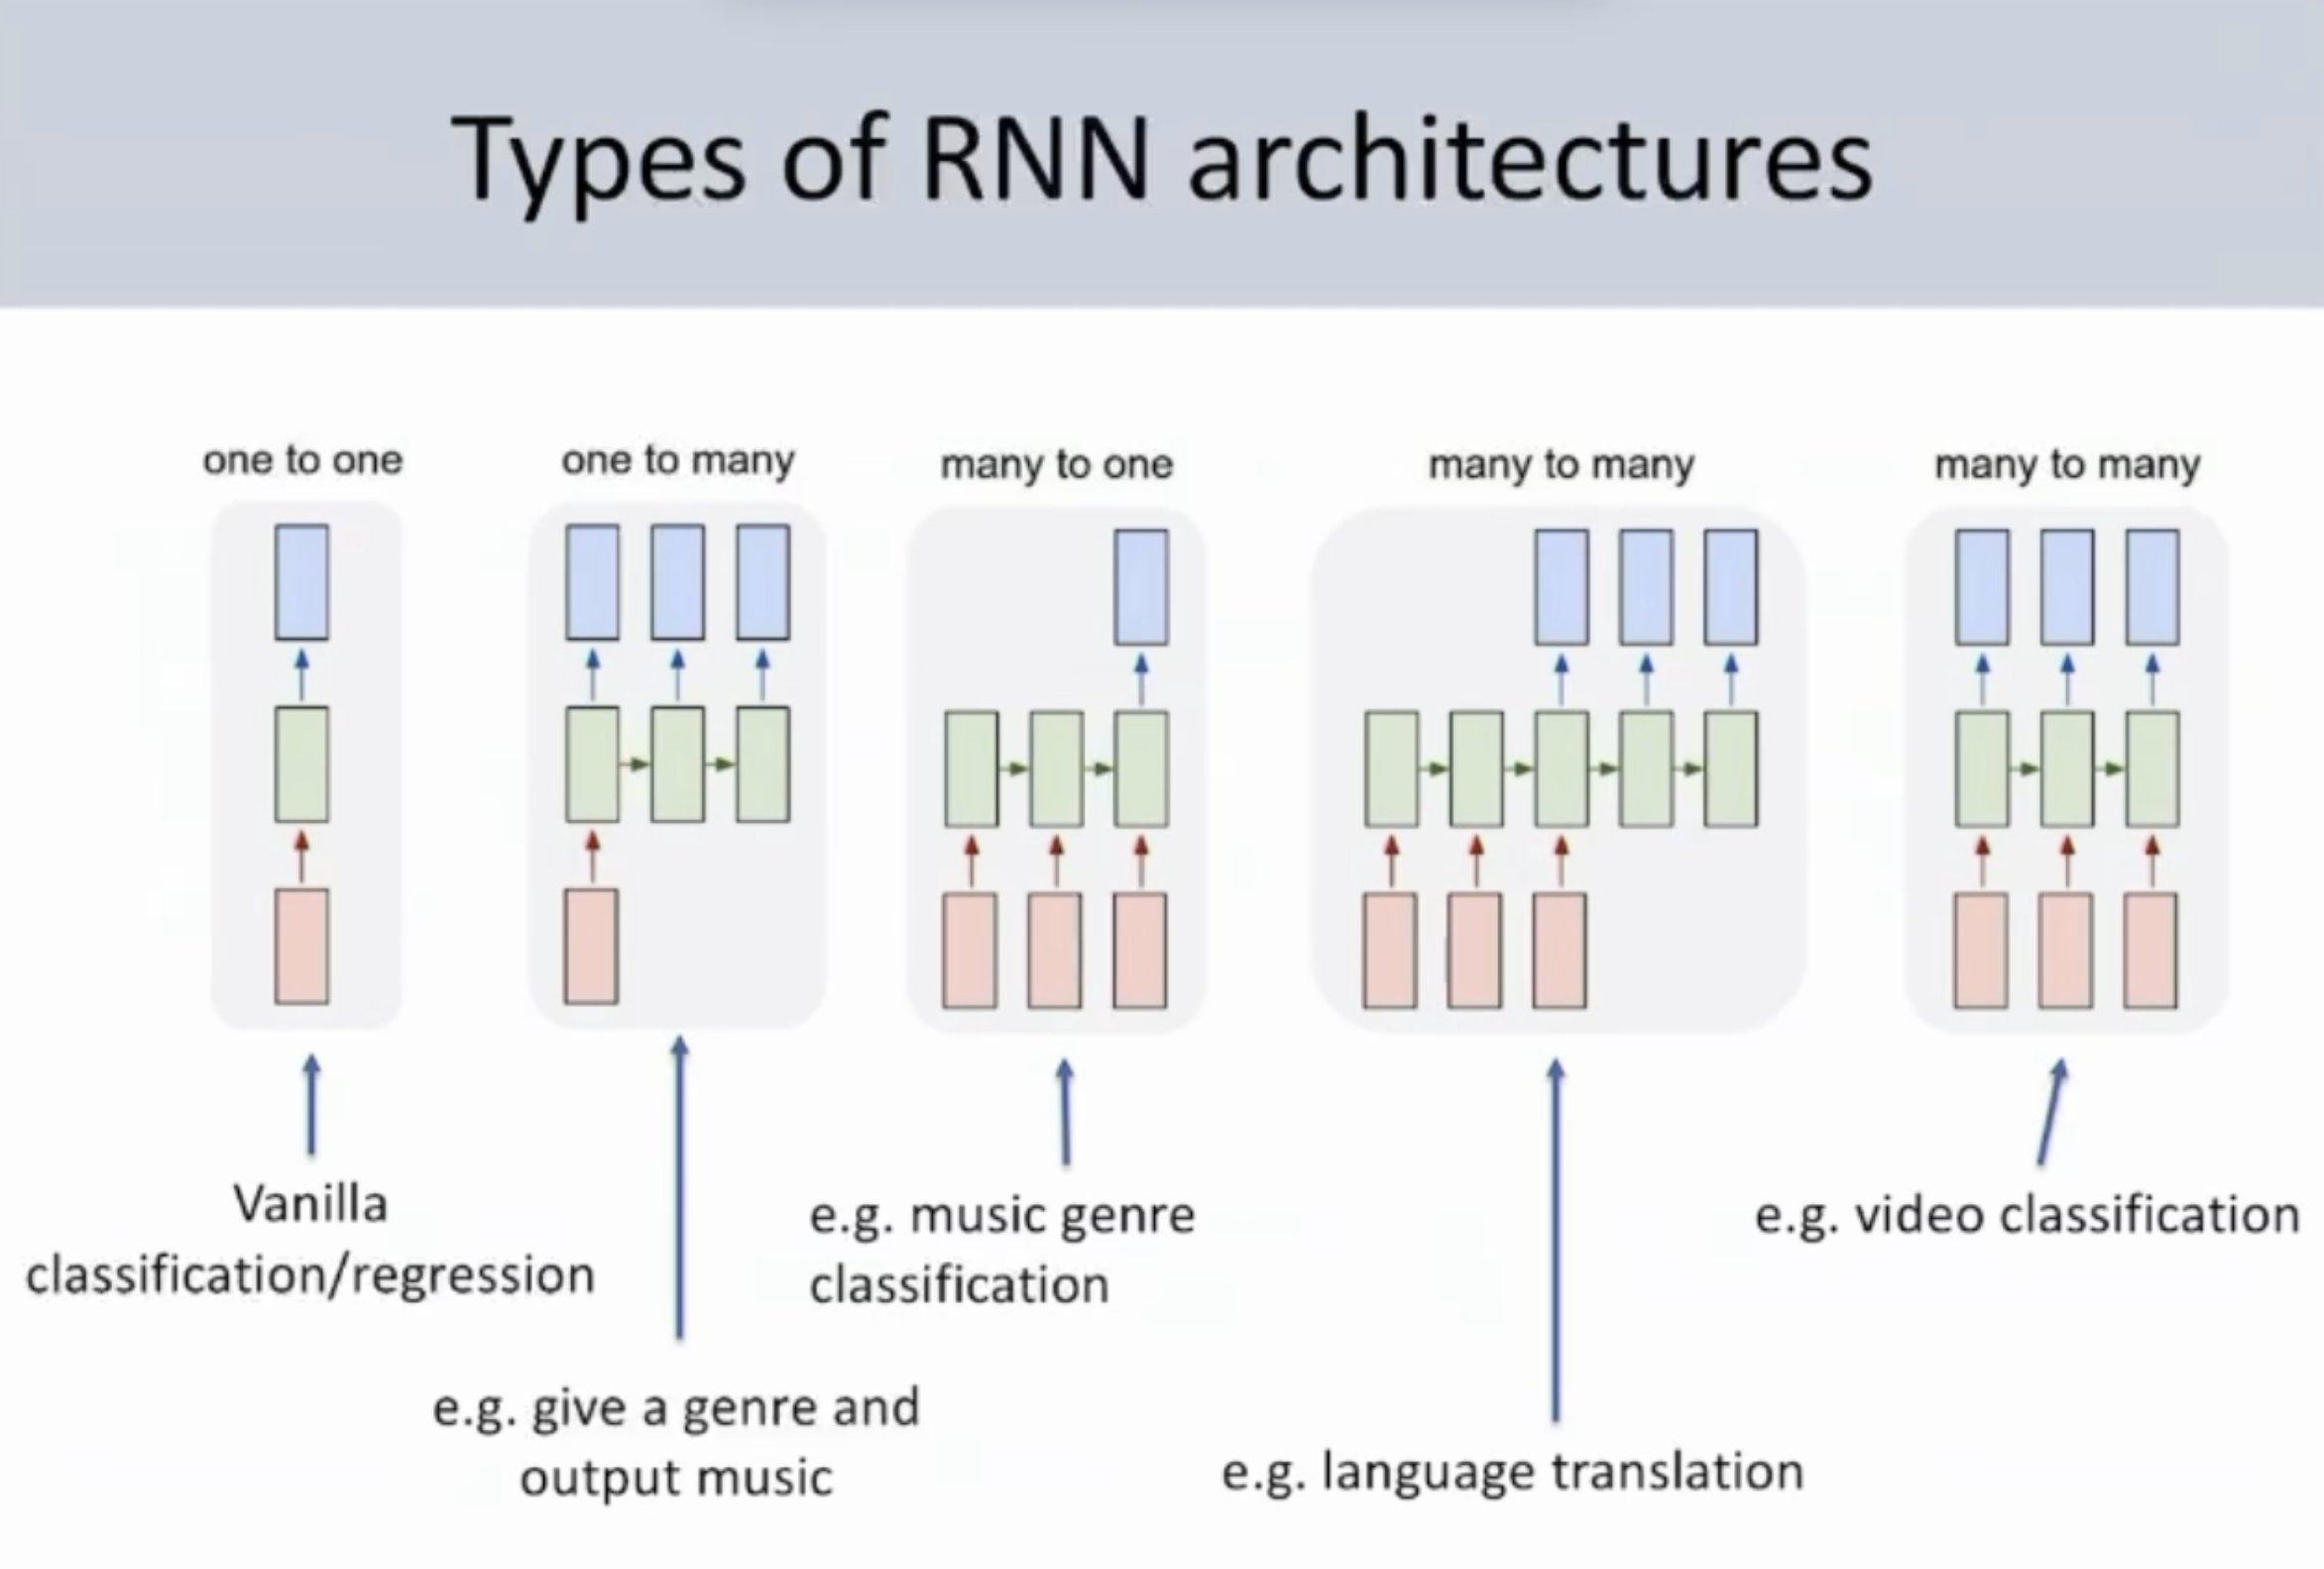
\includegraphics[width=0.75\linewidth]{images/rnn_example_1.png}

\textbf{Desired features}

\begin{itemize}
	\item Efficiently address varying input size
	\item Incorporate dependencies over sequences/time
	\item Allow shared parameters over time
\end{itemize}

\subsection{RNN conceptually}

RNNs have similar features to previous NN. They have layers of neurons, and each layer has forward propagating information. The main unusual/novel thing about RNNs are backwards connections between neurons. These are the main aspects of RNNs that allow them to retain/share infromation over time.

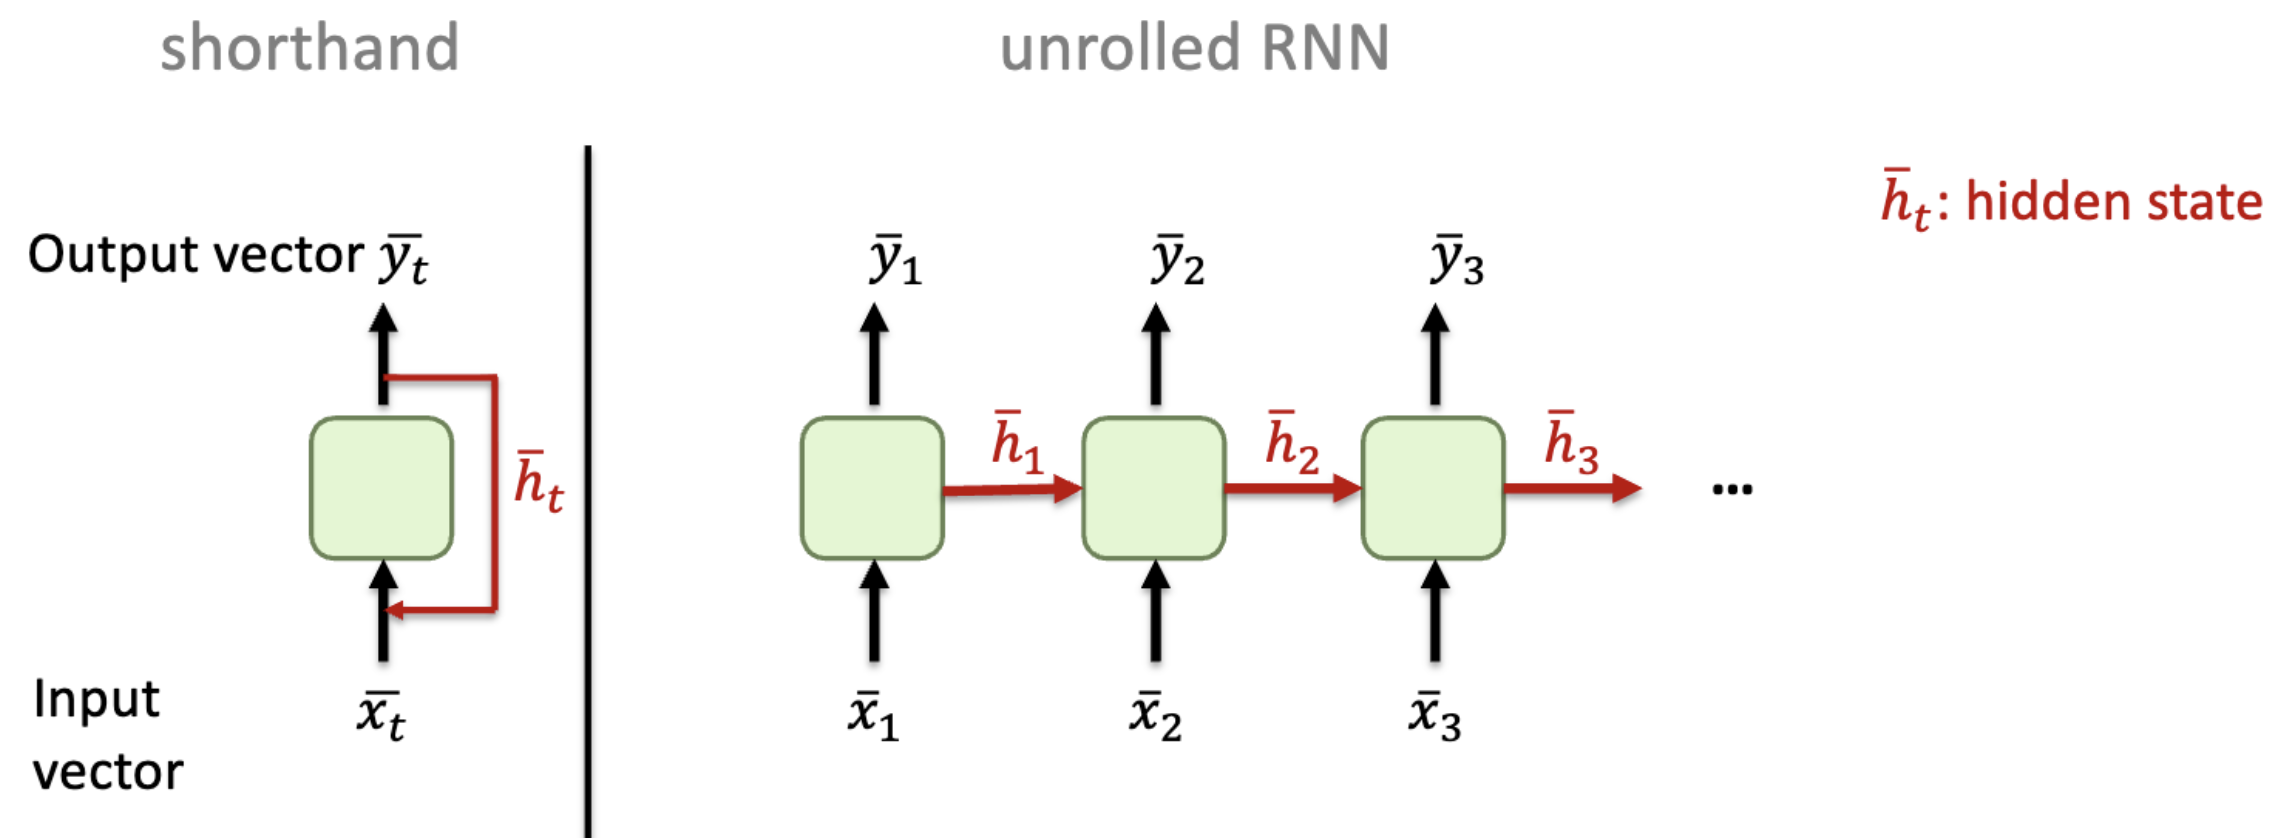
\includegraphics[width=0.75\linewidth]{images/rnn_example_2.png}

Where

\[ \bar h_t = f(\bar h_{t-1}, \bar x_t; W), \quad \bar y_t = g(\bar h_{t-1}, \bar x_t; W) \]

and $f$ and $g$ are functions with learnable parameters (e.g., ffNN). Notice how the $W$ in the functions, which represent the weights in the models, have no $t$ subscript, which means they are time independent. So during our forward pass through the model, the weights in the models are unchanged (all inputs use the same weights).\\

\textbf{Note:} The input vector at $t=1$ (the first input vector) usually takes in a hidden state $h_0$, which is initialized by the architecture or could probably be learnable parameters. This initial state could simply be a zero vector, or it could be specific to bias the architecture towards outputs.

\subsection{Training RNNs}

\begin{itemize}
	\item Initialize prarameters
	\item Forward pass for random input
	\item Backpropagation through time (BPTT). For each timestep (starting with the last timestep), back-propagate through the RNN. This is where the ``through time" comes from.
\end{itemize}

\part{Lecture 15}

\subsection{Overview (revisited)}

Many problems in the human world involve sequences (ex: language translation; input is a sequence of words and output is another sequence of words). Although these problems can be solved by using vanilla NN and CNNs, it becomes very cumbersome to restate the problems to be effectively solved using these previous architectures. Additionally, getting these previous architectures to really understand the notion of a sequence (where previous input/output affects the next output) is much more problematic than using an architecture with this notion designed into the architecture.\\

On top of this new notion of sequences that we want to learn, we also have tasks that have different combinations of sequences in their inputs and outputs:

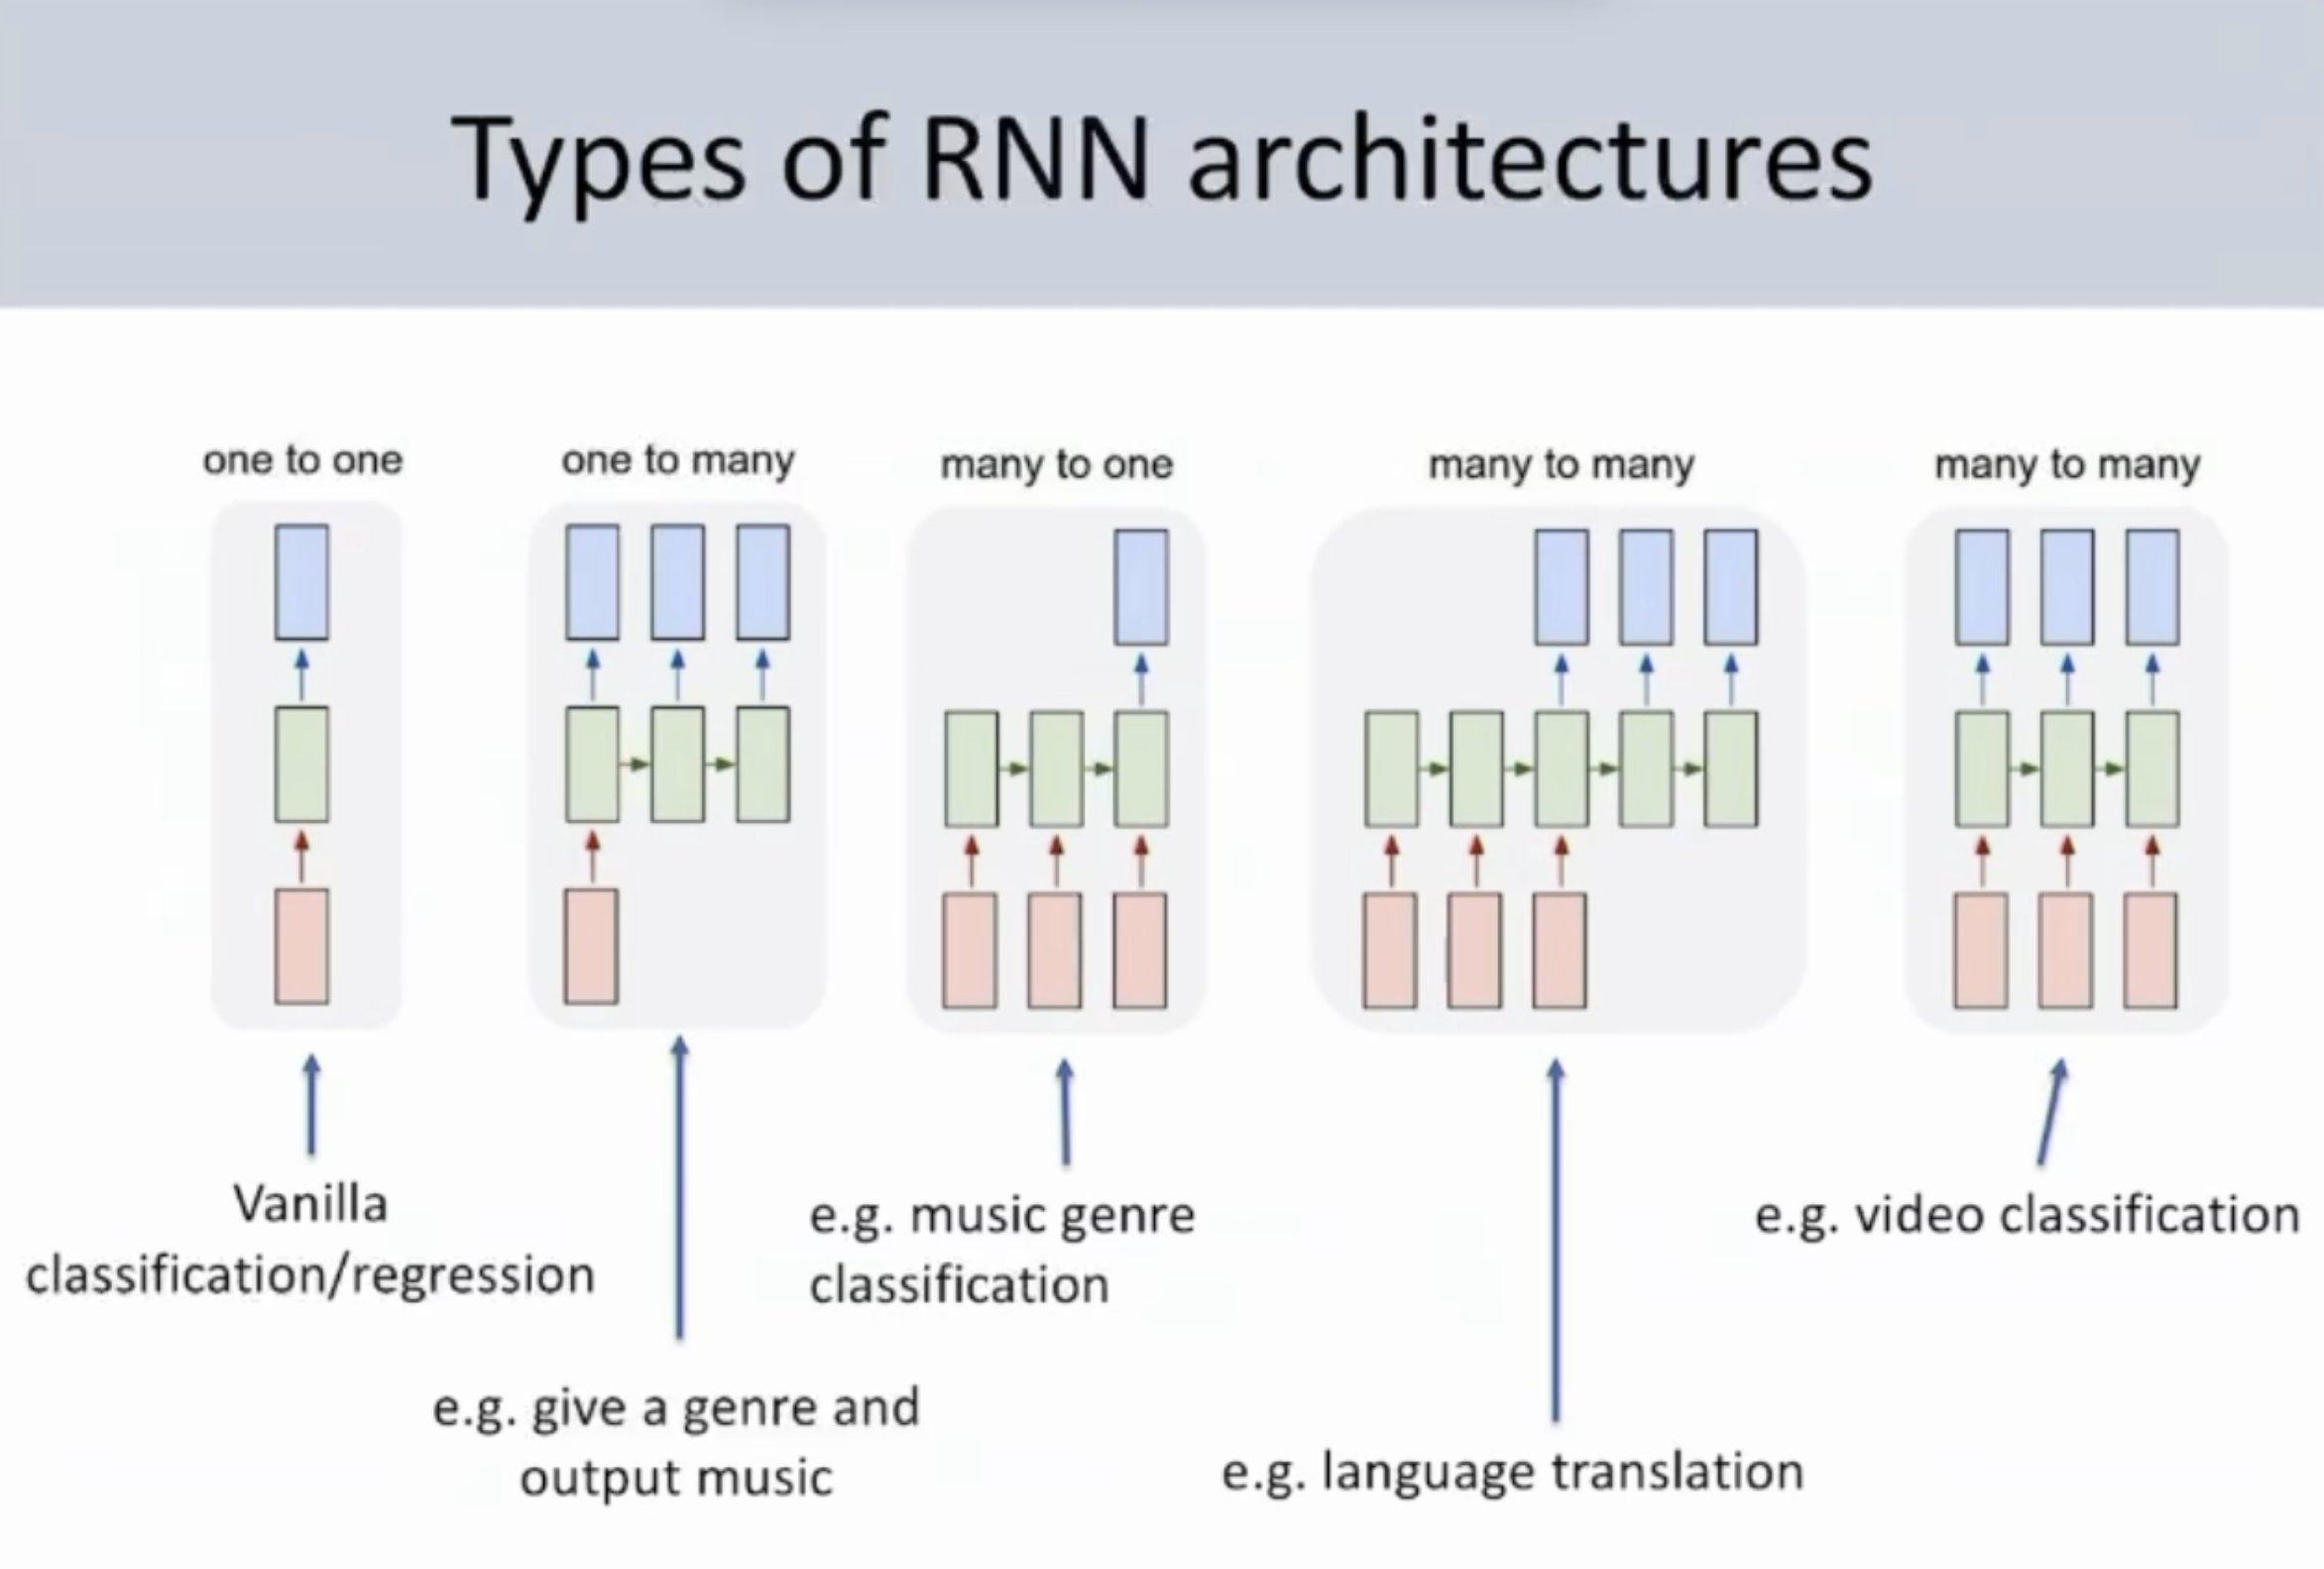
\includegraphics[width=0.75\linewidth]{images/rnn_example_1.png}\\
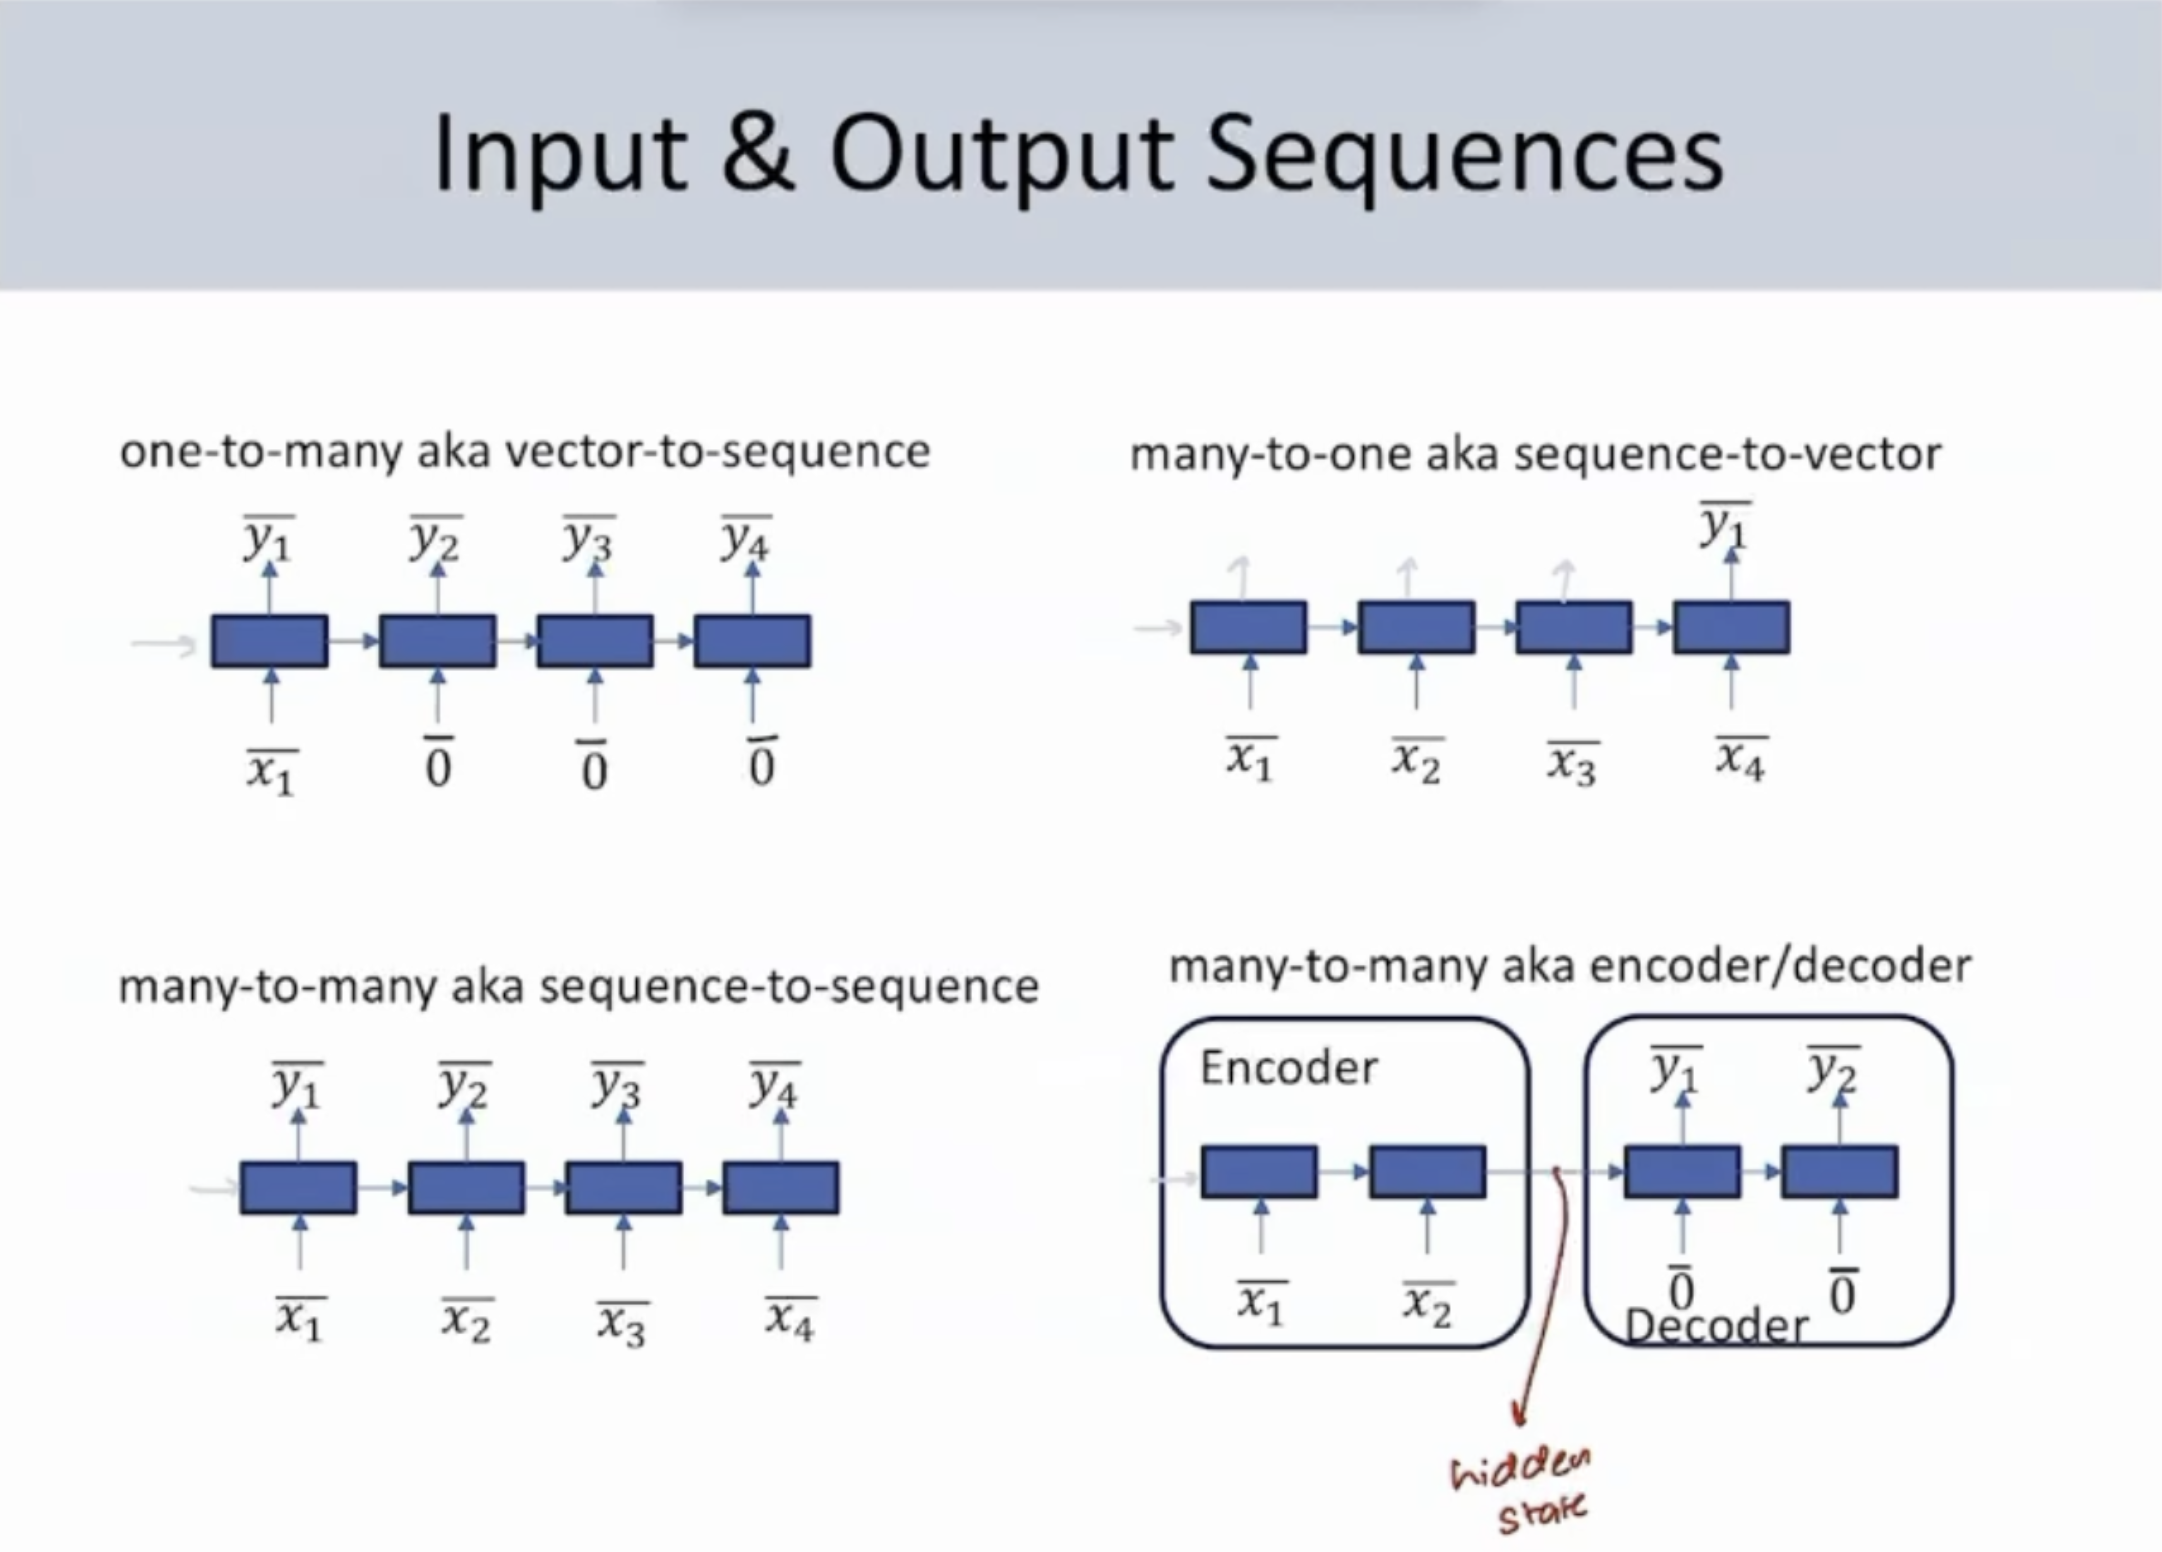
\includegraphics[width=0.75\linewidth]{images/rnn_example_8.png}\\

One interesting task is language translation, which has a special many to many architecture (input is a sequence and output is a sequence) that has an output only after a certain sequence has been read. With this in mind, we might want to encode some information into our architecture to effectively do this type of task, which we can see is the hidden state passed between the encoder and decoder section. However, similar to cons listed in section 26.6, this encoded information could contain heavily diluted information from many timesteps ago, leading to poor long-term dependencies.\\

Another thing of note is that the weights for each of the blue boxes in any of the given models must be the exact same, except for the many-to-many encoder/decoder model which can have two seperate weights, one for the encoder and one for the decoder. This makes sense because you are reusing the same model for each element in a sequence, which is clear from the shorthand version in section 26.2. If this weren't the case, the model could not take in a variable sequence length, which would be a huge drawback.

\subsection{RNN: example}

The first thing to understand is that inputs (and outputs) of an RNN model at each timestep are usually a vector, even though they are technically one single element of a sequence. We can take an element and make it into a vector through many forms of encoding, but one very basic way is through one-hot encoding:\\

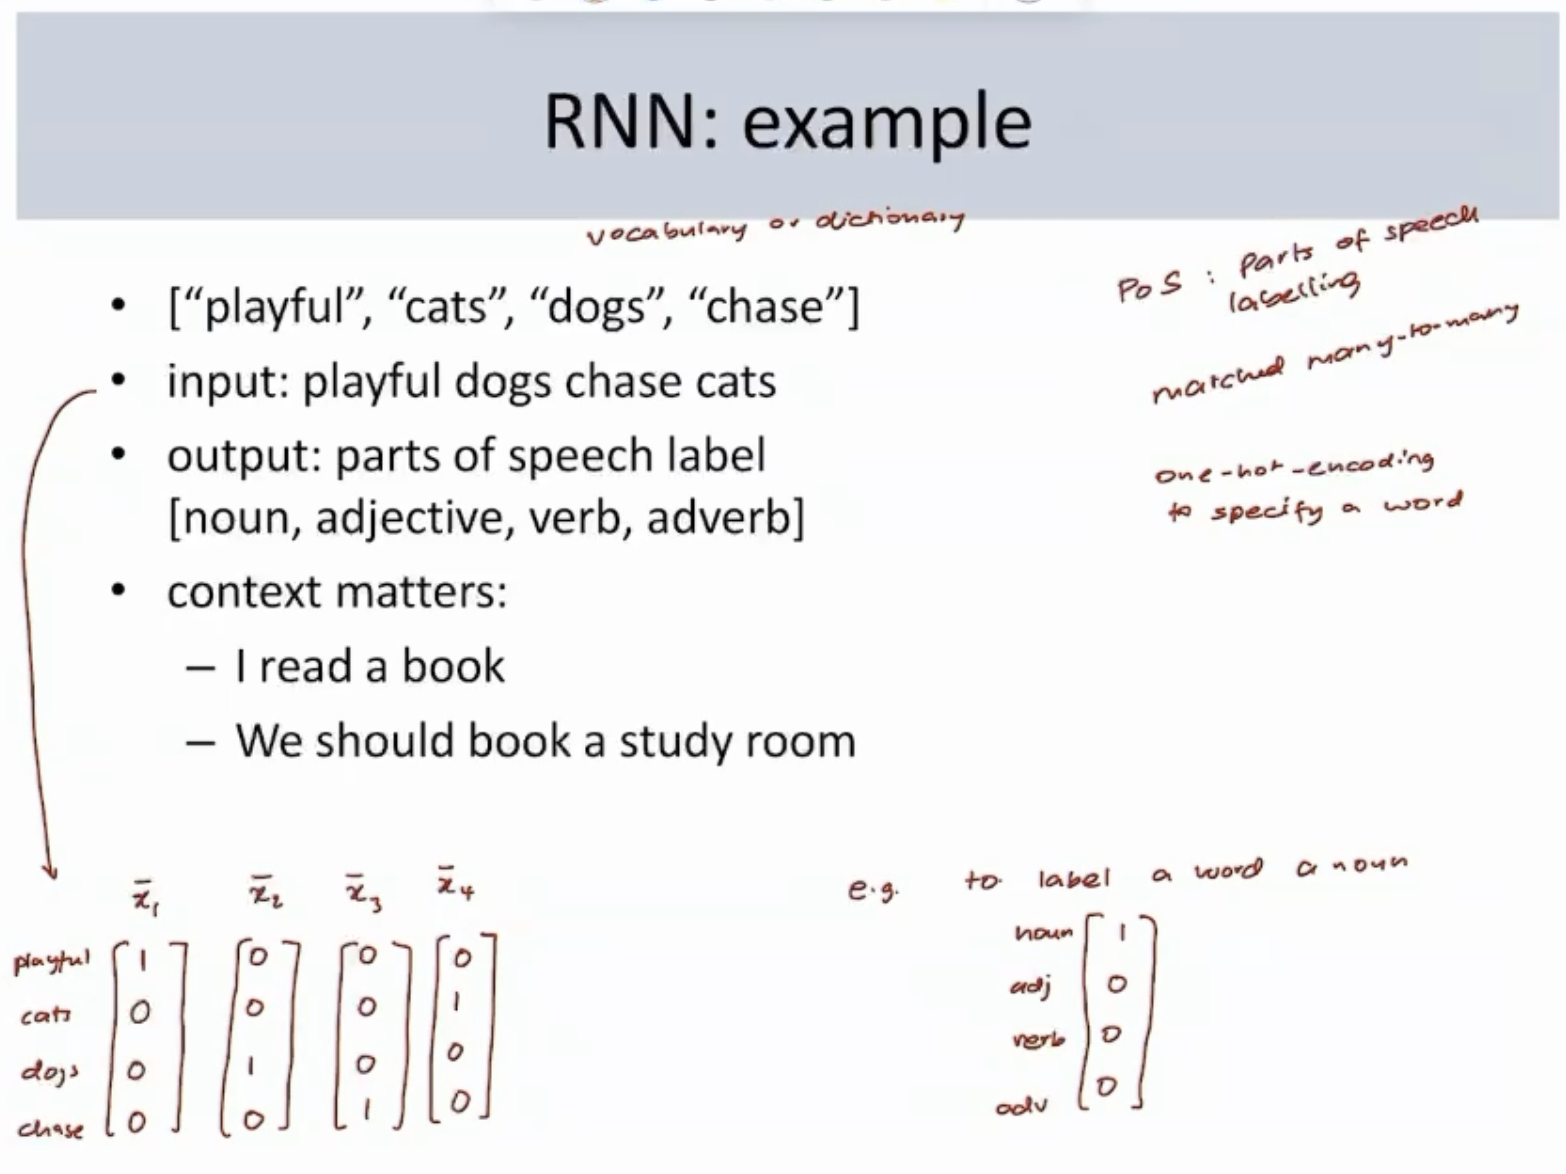
\includegraphics[width=0.75\linewidth]{images/rnn_example_3.png}\\

In this example, we have a preset dictionary of words [playful, cats, dogs, chase]. If our input is ``playful dogs chase cats", we transform this input into 4 vectors $\bar x_1, \bar x_2, \bar x_3, \bar x_4$ listed above. Since this is a matched many-to-many example, we have output $\bar y_1, \bar y_2, \bar y_3, \bar y_4$ corresponding to each input element. These outputs are also a vector, which we again encode through one-hot encoding of a list of parts of speech labels [noun, adjective, verb, adverb].\\

Now lets look at how the architecture might look like for this example:\\

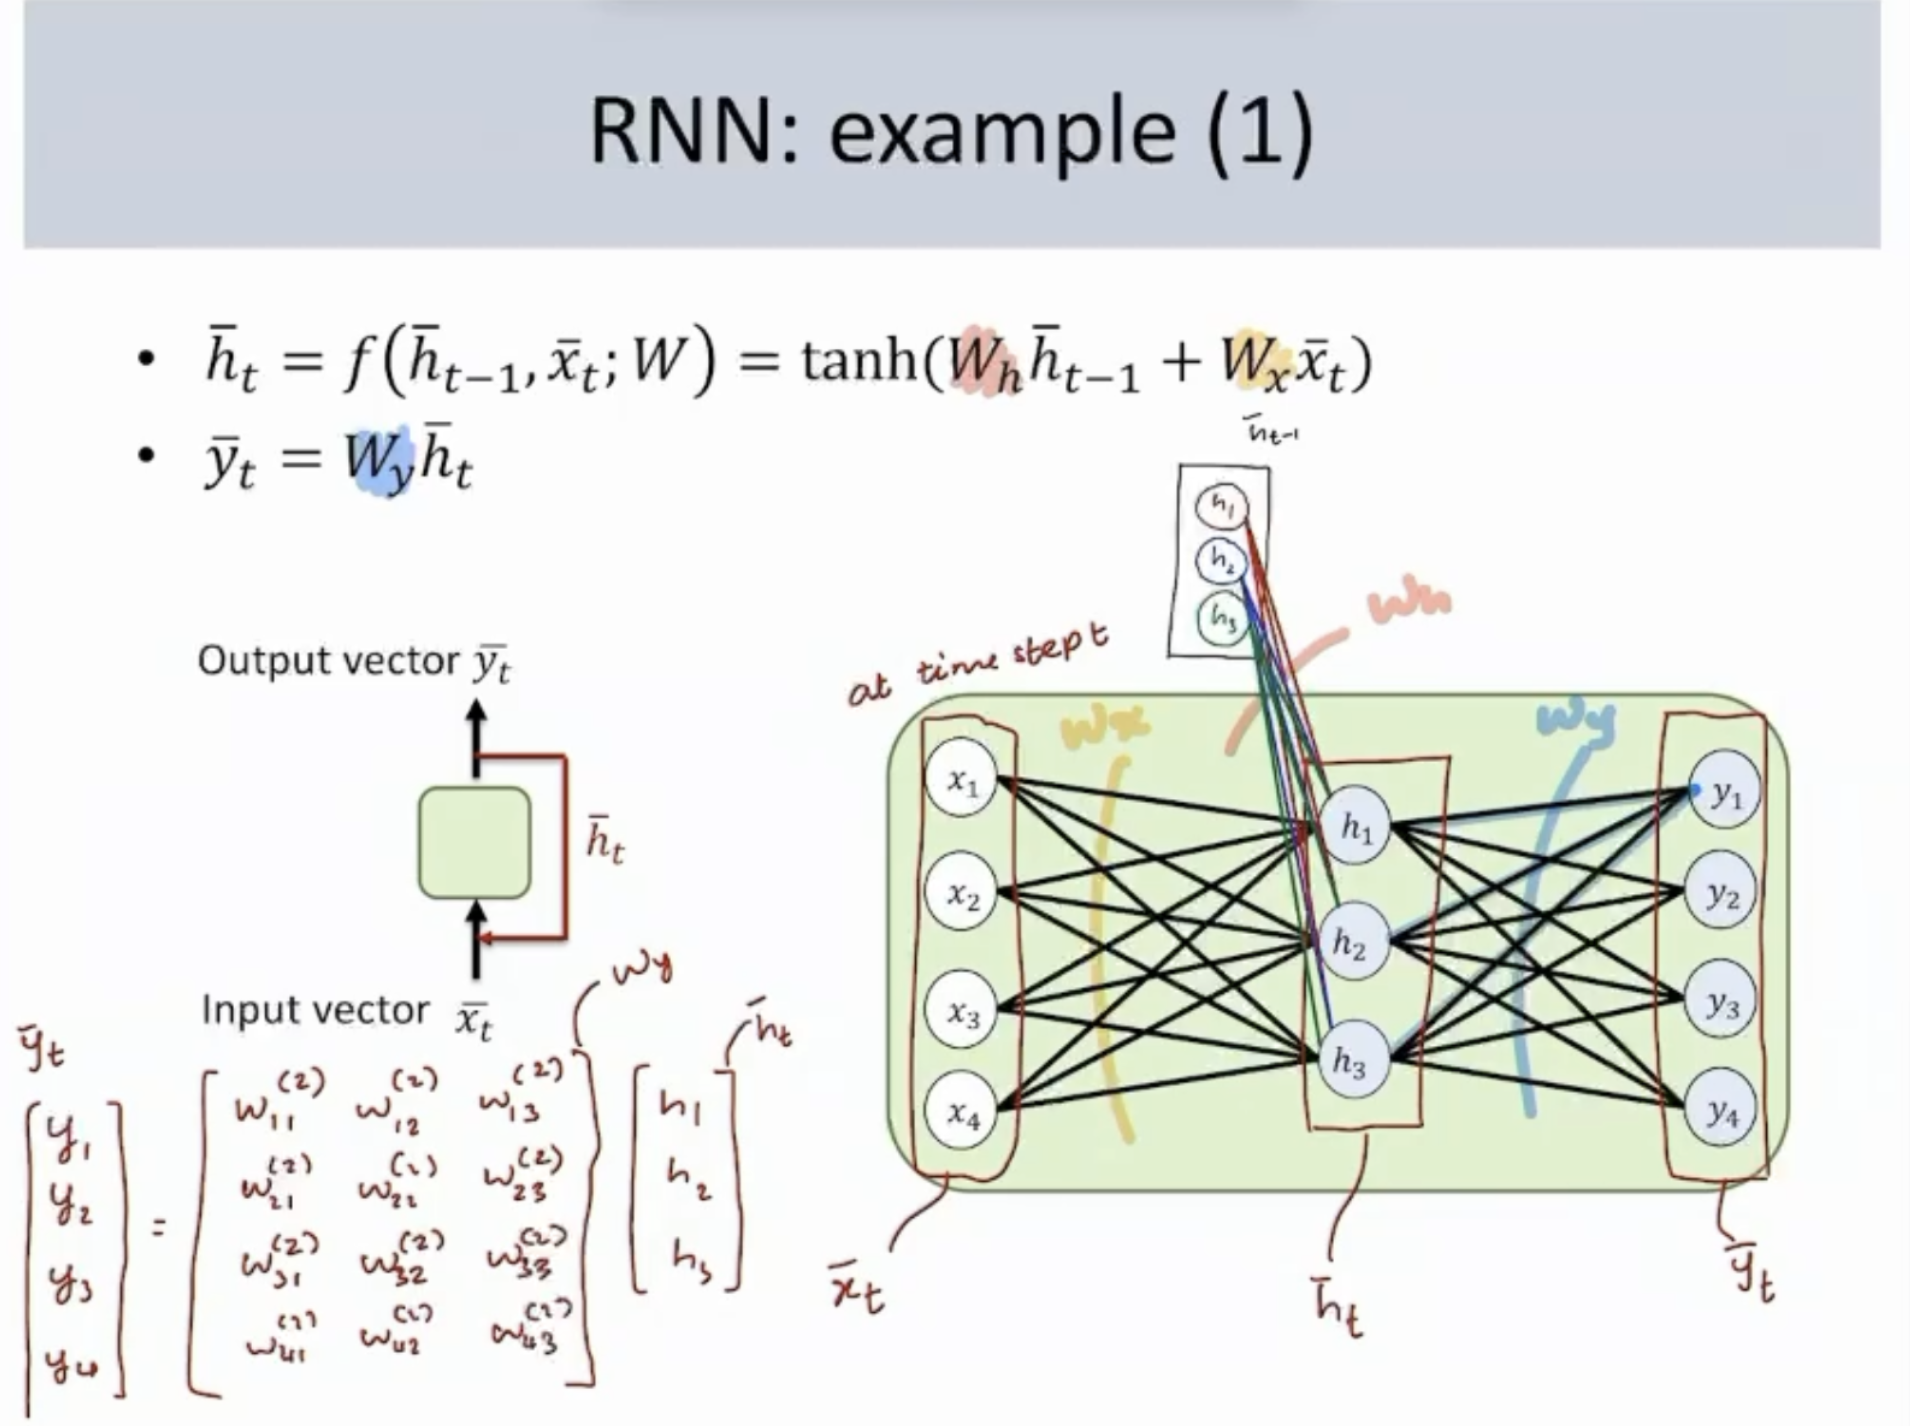
\includegraphics[width=0.75\linewidth]{images/rnn_example_4.png}\\

\textbf{Note:} The model in the green box represents the $f$ and $g$ functions that we talked about before, and could be any model with learnable parameters. In this case, it is a fully-connected Neural Network, but not necessarily a feed forward one because there much be connections backwards between $\bar h$s to retain information between input vectors.\\

Given that we already learned our weights:\\

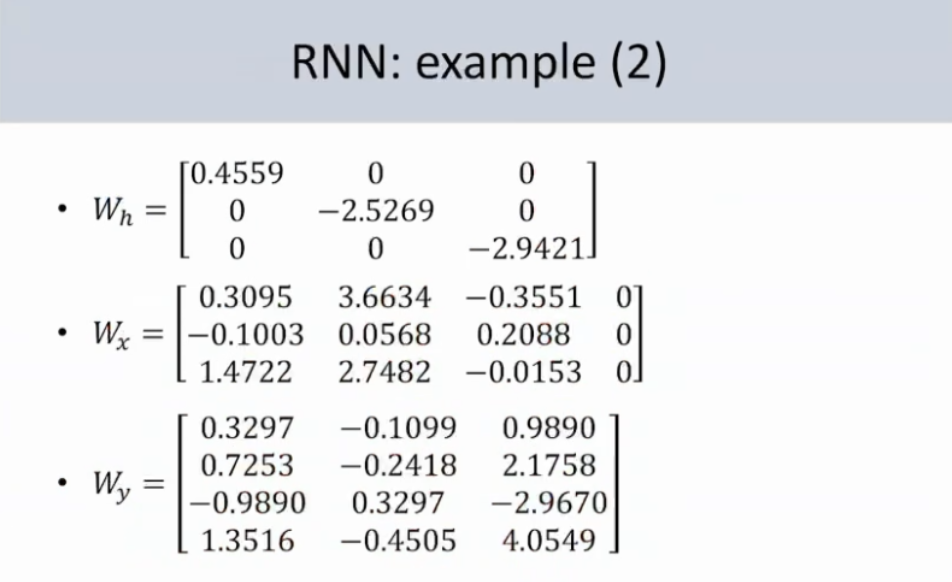
\includegraphics[width=0.75\linewidth]{images/rnn_example_5.png}\\

We then calculate our guess for our first input:

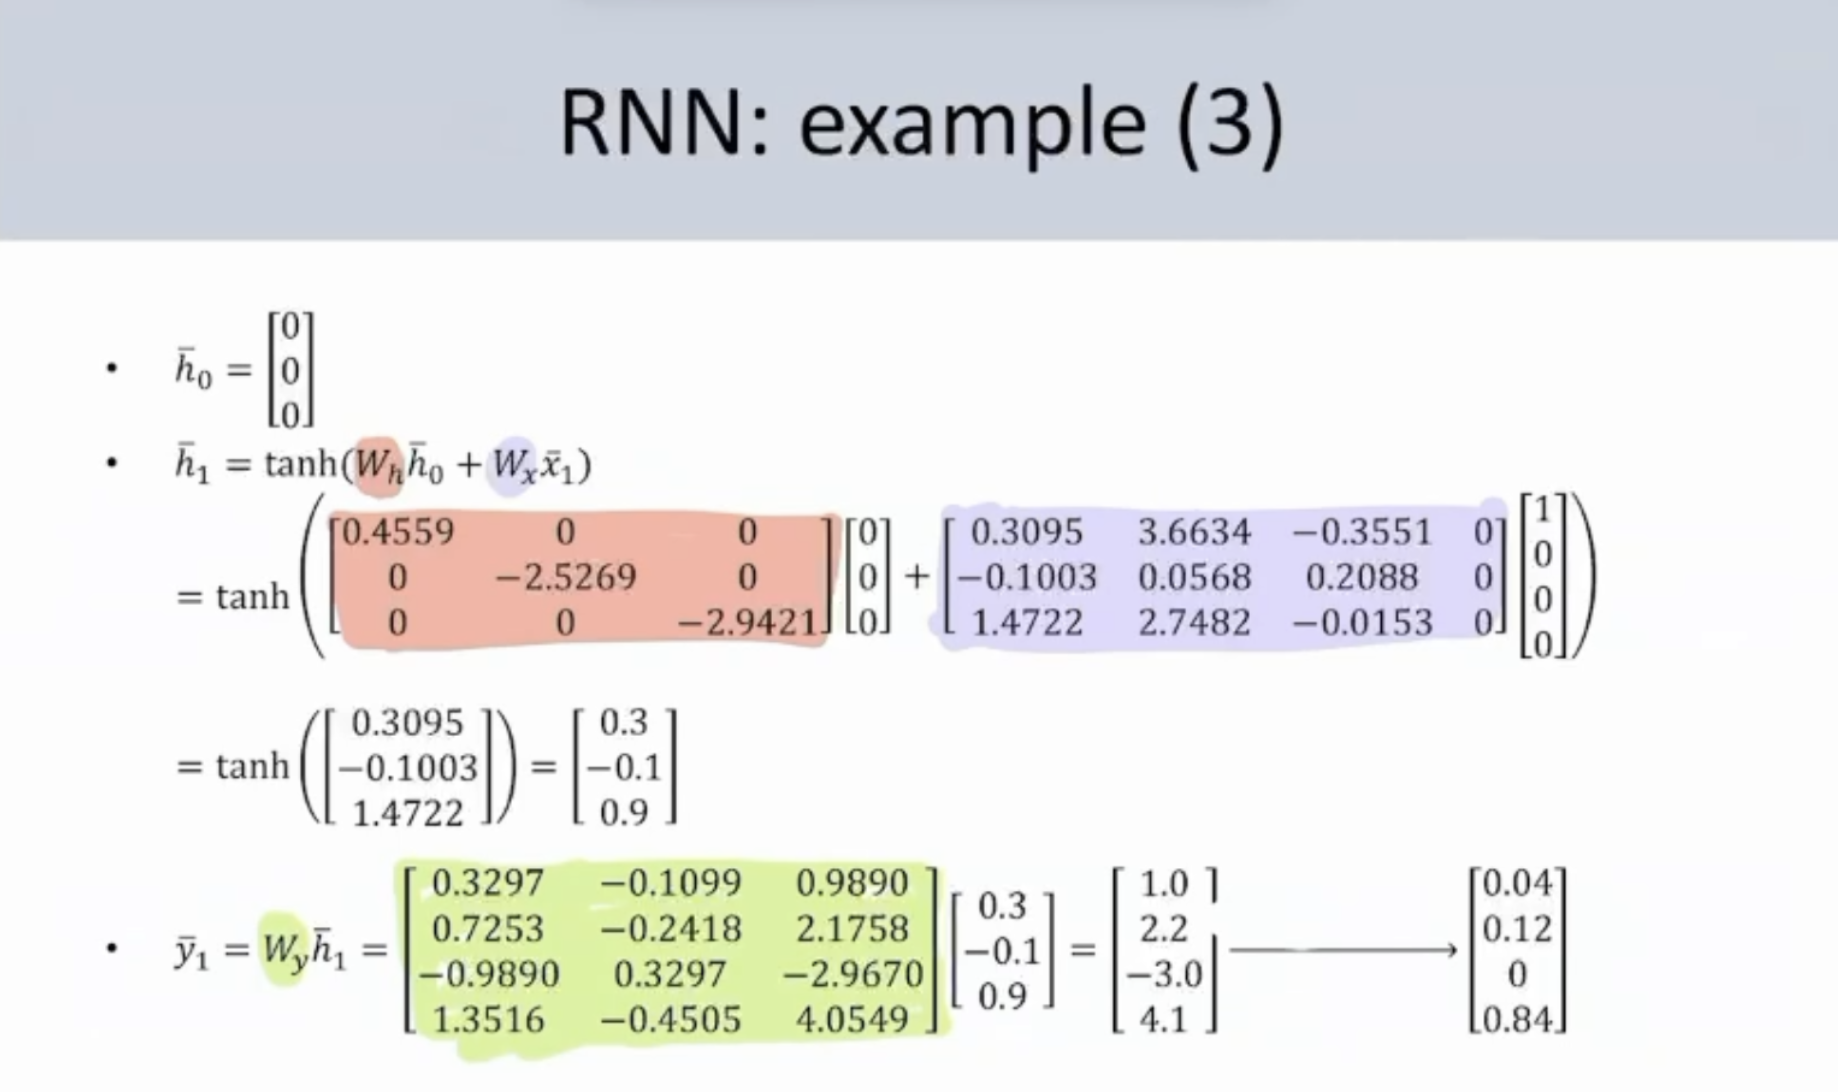
\includegraphics[width=0.75\linewidth]{images/rnn_example_6.png}\\

Notice that we initialize our hitten state to $\bar 0$. To make our prediction for the first input, we take the softmax of the output $\bar y_1$. We then continue to our second input:\\

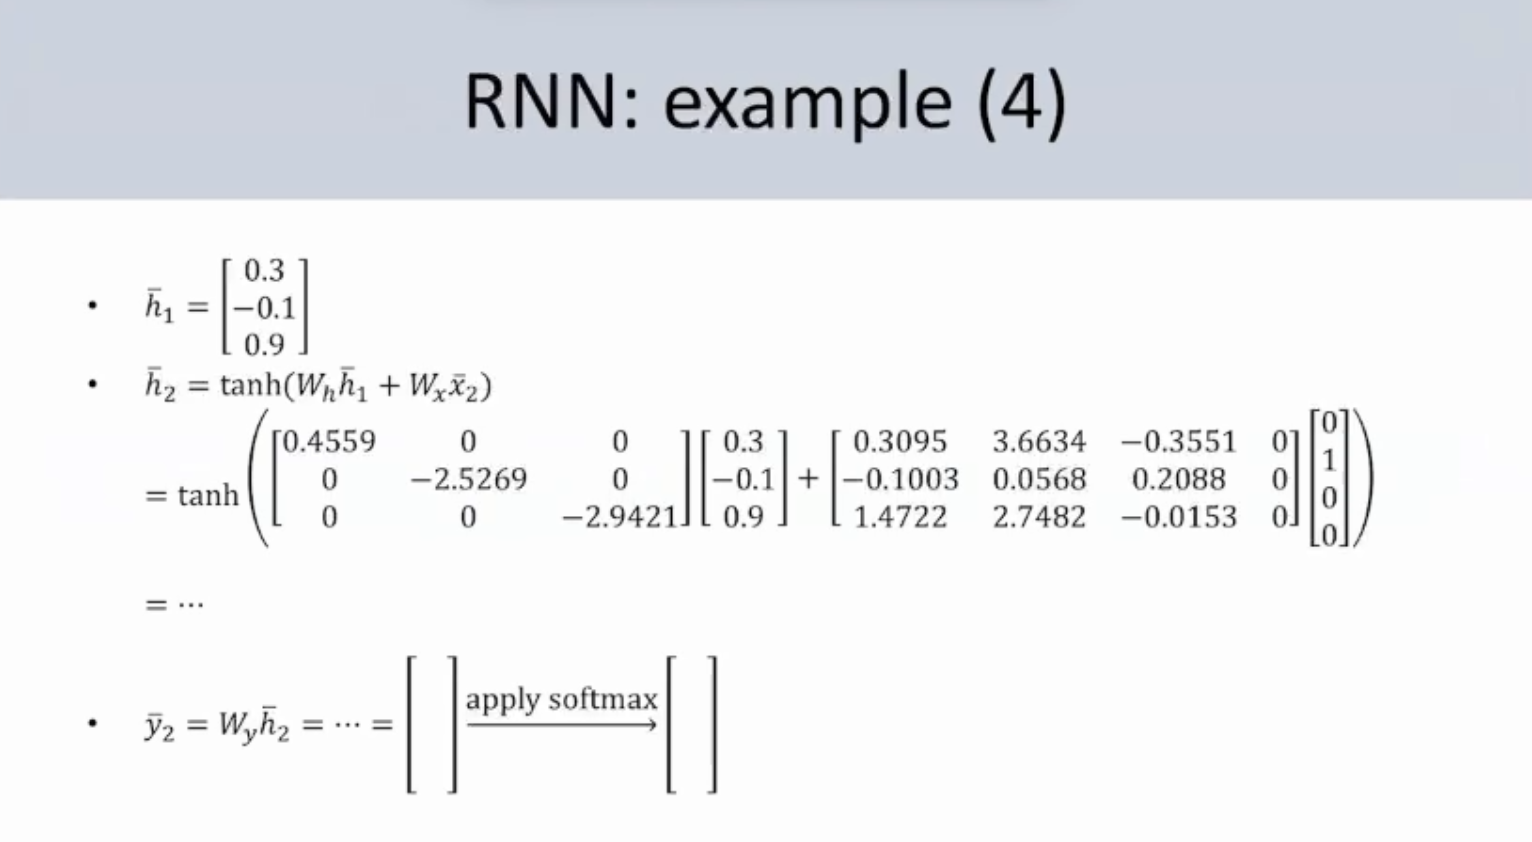
\includegraphics[width=0.75\linewidth]{images/rnn_example_7.png}\\

Our prediction for our second input follows very similar steps to our prediction for our first input, with the only difference being that we use $\bar h_1$ as our hidden state instead of $\bar h_0$.

\subsection{RNNs: Pros and Cons} 

\textbf{Pros:}

\begin{itemize}
	\item Incorporate dependencies over time
	\item Can handle sequences with variable lengths
	\item Model size doesn't increase for longer input
\end{itemize}

\textbf{Cons}

\begin{itemize}
	\item No paralleization: has to do recurrent, dependent computation
	\item Bad at long-term memory: vanishing gradient - In your BPTT, you typically have a term 
		\[ \prod_{t=2}^T \pdv{h_t}{h_{t-1}}\]
		If we look back at how back-propagation works in equation \ref{eq:two layer nn with sgd 3} in the original two layer NN example, we can extrapolate to see how this term is created for weight updates that connect information far apart in time. This is especially detrimental to NN that use the $\tanh$ activation function because the derivative is always $\le 1.0$. Thus, weight updates that occur through inaccuracies in relations between information far apart in time are essentially 0.
\end{itemize}

\part{Lecture 16}

\section{Long-Short Term Memory}

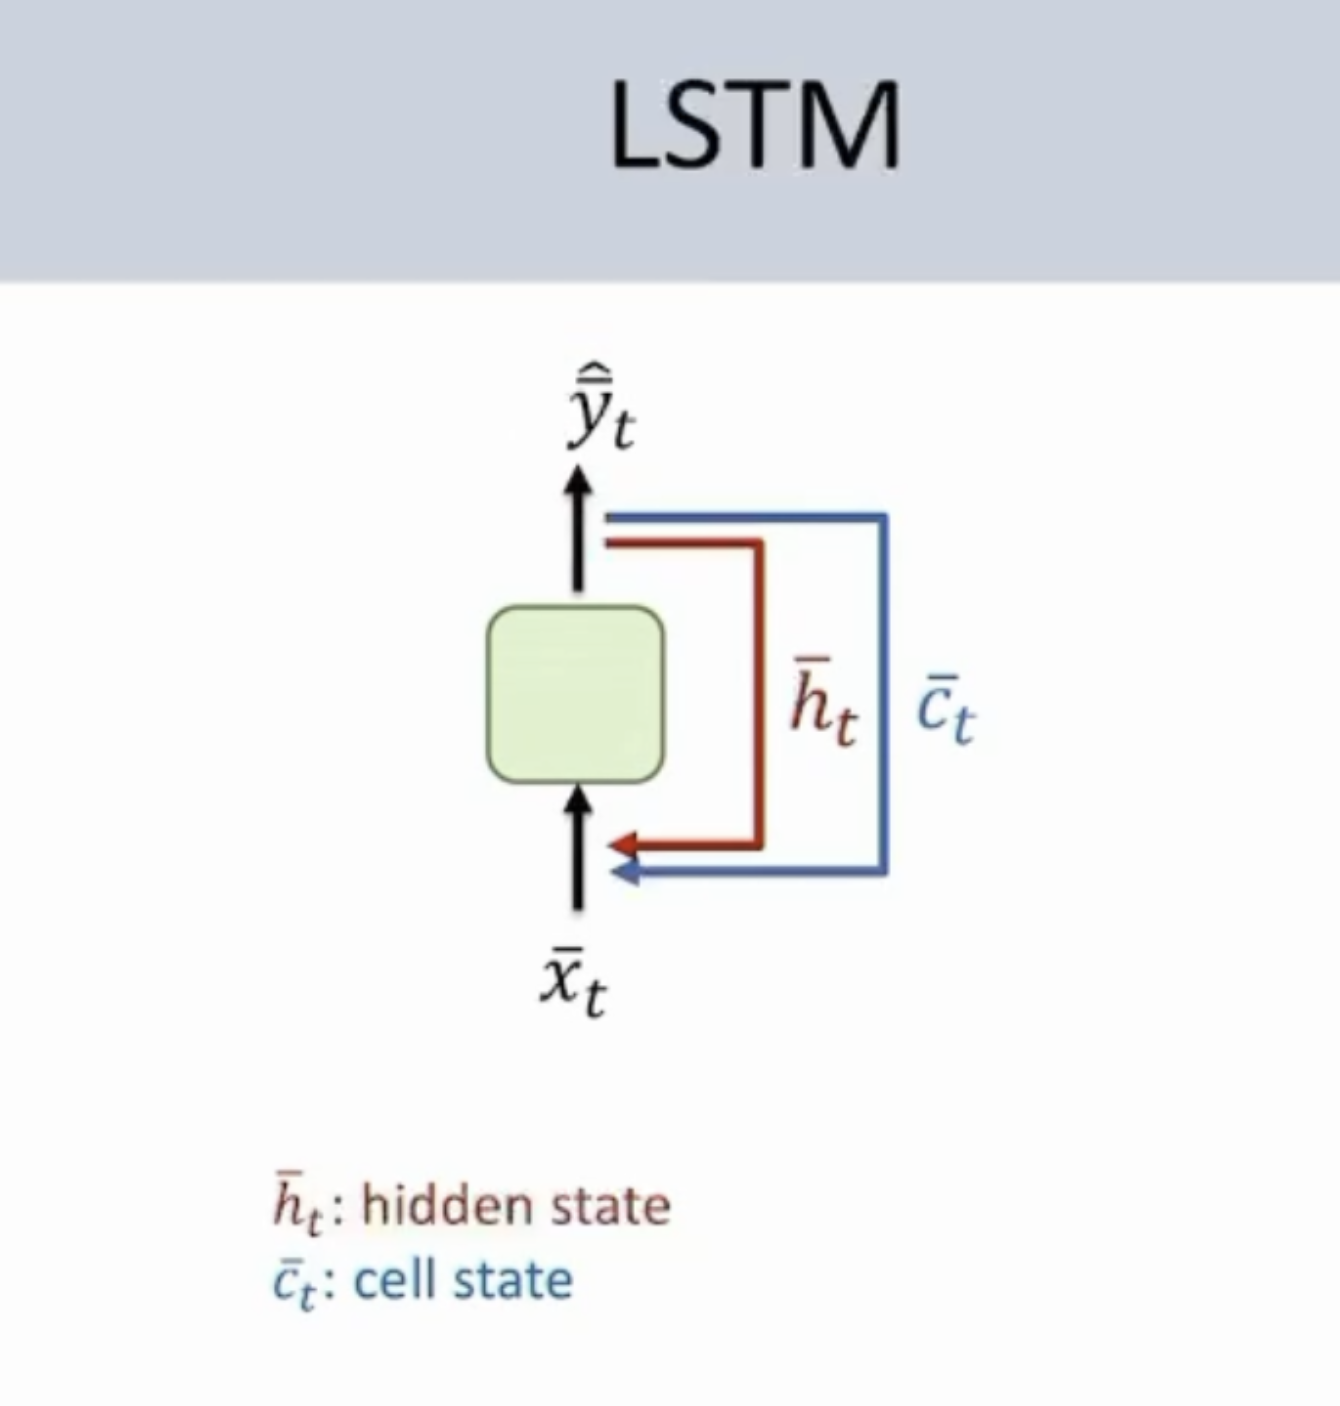
\includegraphics[width=0.75\linewidth]{images/lstm_example_1.png}\\

Similar to RNNs, LSTMs output an output vector $\bar y_t$ and a hidden state vector $\bar h_t$ for each timestep. It also outputs a new vector, $\bar c_t$, which is meant to encode long-term memory. This new vector is typically referred to as \textbf{cell state}. So now we have two types of memories, short-term and long-term memory, which is similar to how we humans remember information. These two memories are clearly going to be encoded differently from each other.

\subsection{LSTM unit}

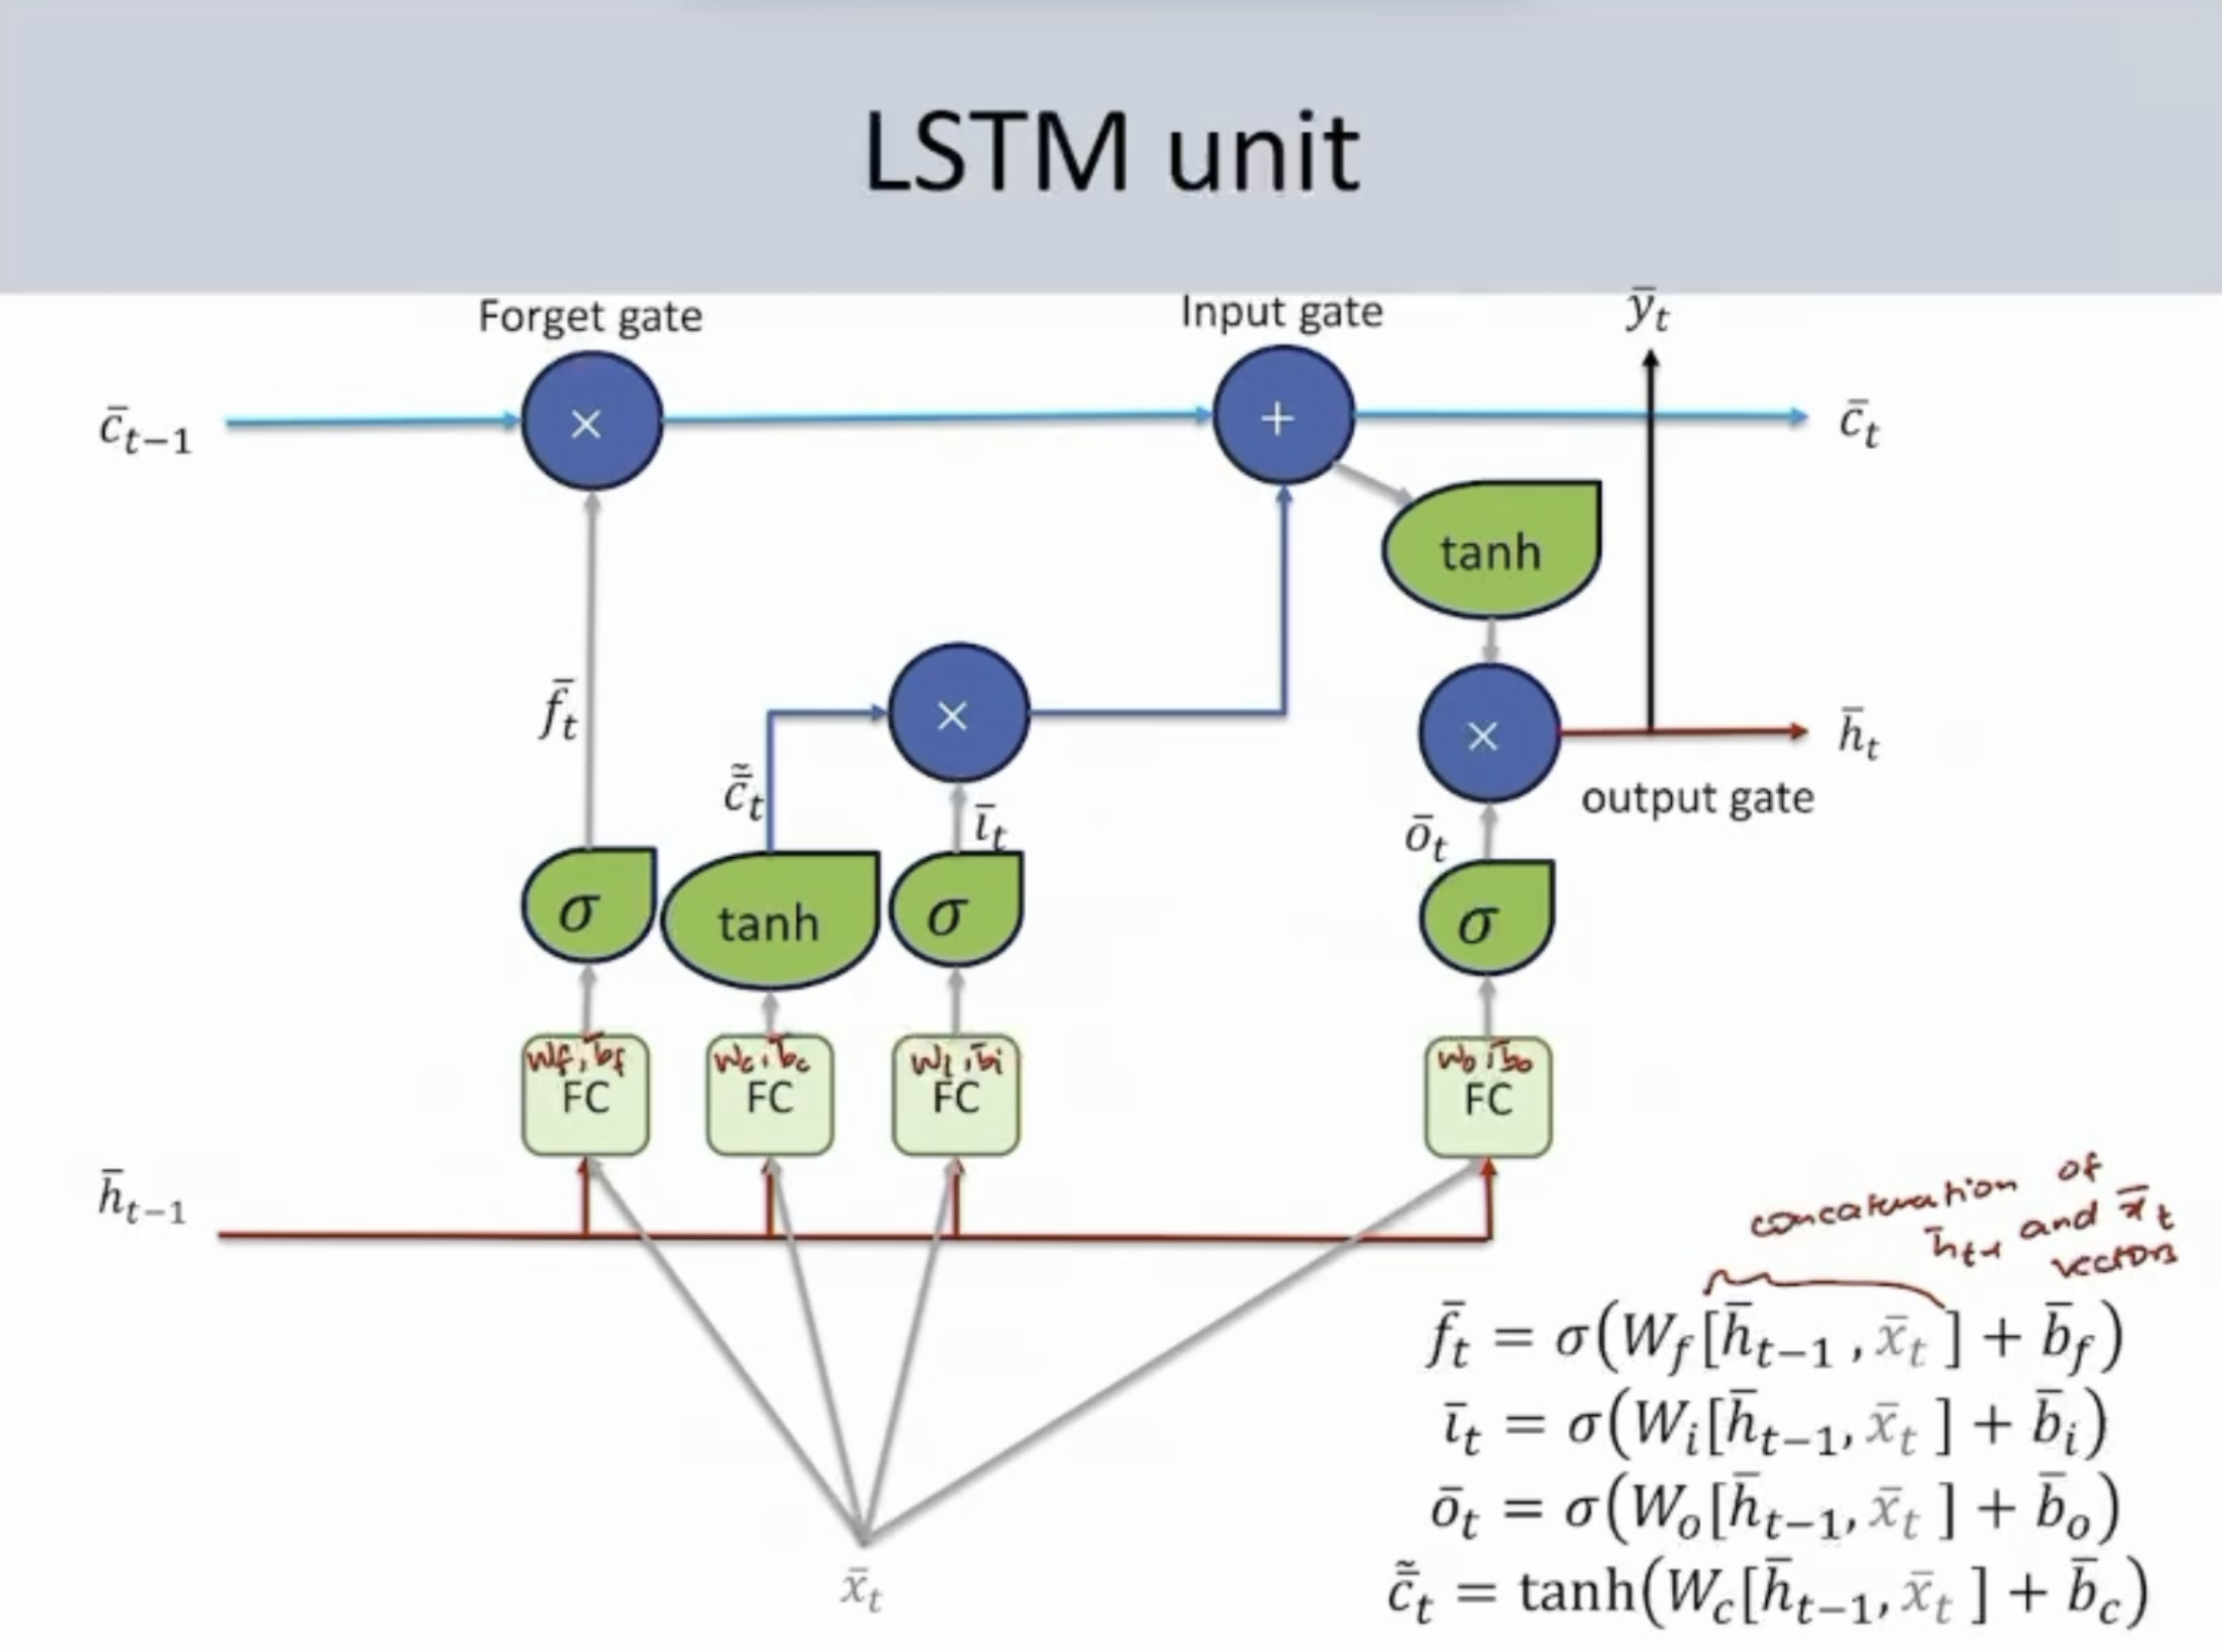
\includegraphics[width=0.75\linewidth]{images/lstm_example_3.png}\\

The $\times$ cells in this picture represent element-wise multiplication (hadamard product) and the $+$ cells represent element-wise plus. Remember that the $\sigma$ function squishes the input into a value in the range $[0, 1]$ and the $\tanh$ function squishes the input into a value in the range $[-1, 1]$.\\

\textbf{Note:} You could use an activation function (ex. soft max) instead of taking $\bar h_t$ directly as the output

\subsection{Forget Gate}

The forget gate takes the old long term memory $\bar c_{t-1}$ and filters the important memory by multiplying it with a vector that has passed through the $\sigma$ function (values between $[0,1]$). This product effectively retains the important elements of $\bar c_{t-1}$ by multiplying them with a value near $1$ and forget the unimportant elements by multiplying them with a value near $0$.


\subsection{Input Gate}

The input gate takes in freshly forgotten form of $\bar c_{t-1}$ and adds it with a second vector that represents the change to long term memory from this timestep. This second vector is the product of two vectors, $\tilde{\bar c}_t$ and $\bar l_t$. $\tilde{\bar c}_t$ has passed through the $\tanh$ function (values between $[-1, 1]$) and $\bar l_t$ has passed through the $\sigma$ function (values between $[0, 1]$). $\tilde{\bar c}_t$ represents the raw updates that $\bar h_{t-1}$ and $\bar x_t$ have on $\bar c_t$, and $\bar l_t$ represents the filtered impact that these updates should have. 

\subsection{Input Gate}

The output gate takes in the final version of our long term memory $\bar c_t$ after all its updates, and filters it using the old short-term memory $\bar h_{t-1}$ and the input $\bar x_t$. The output of this game is the state of the new short-term memory. This means that the states of short-term memory are essentially filtered versions of long-term memory, which kinda makes sense. 

\subsection{Encoder/Decoder}

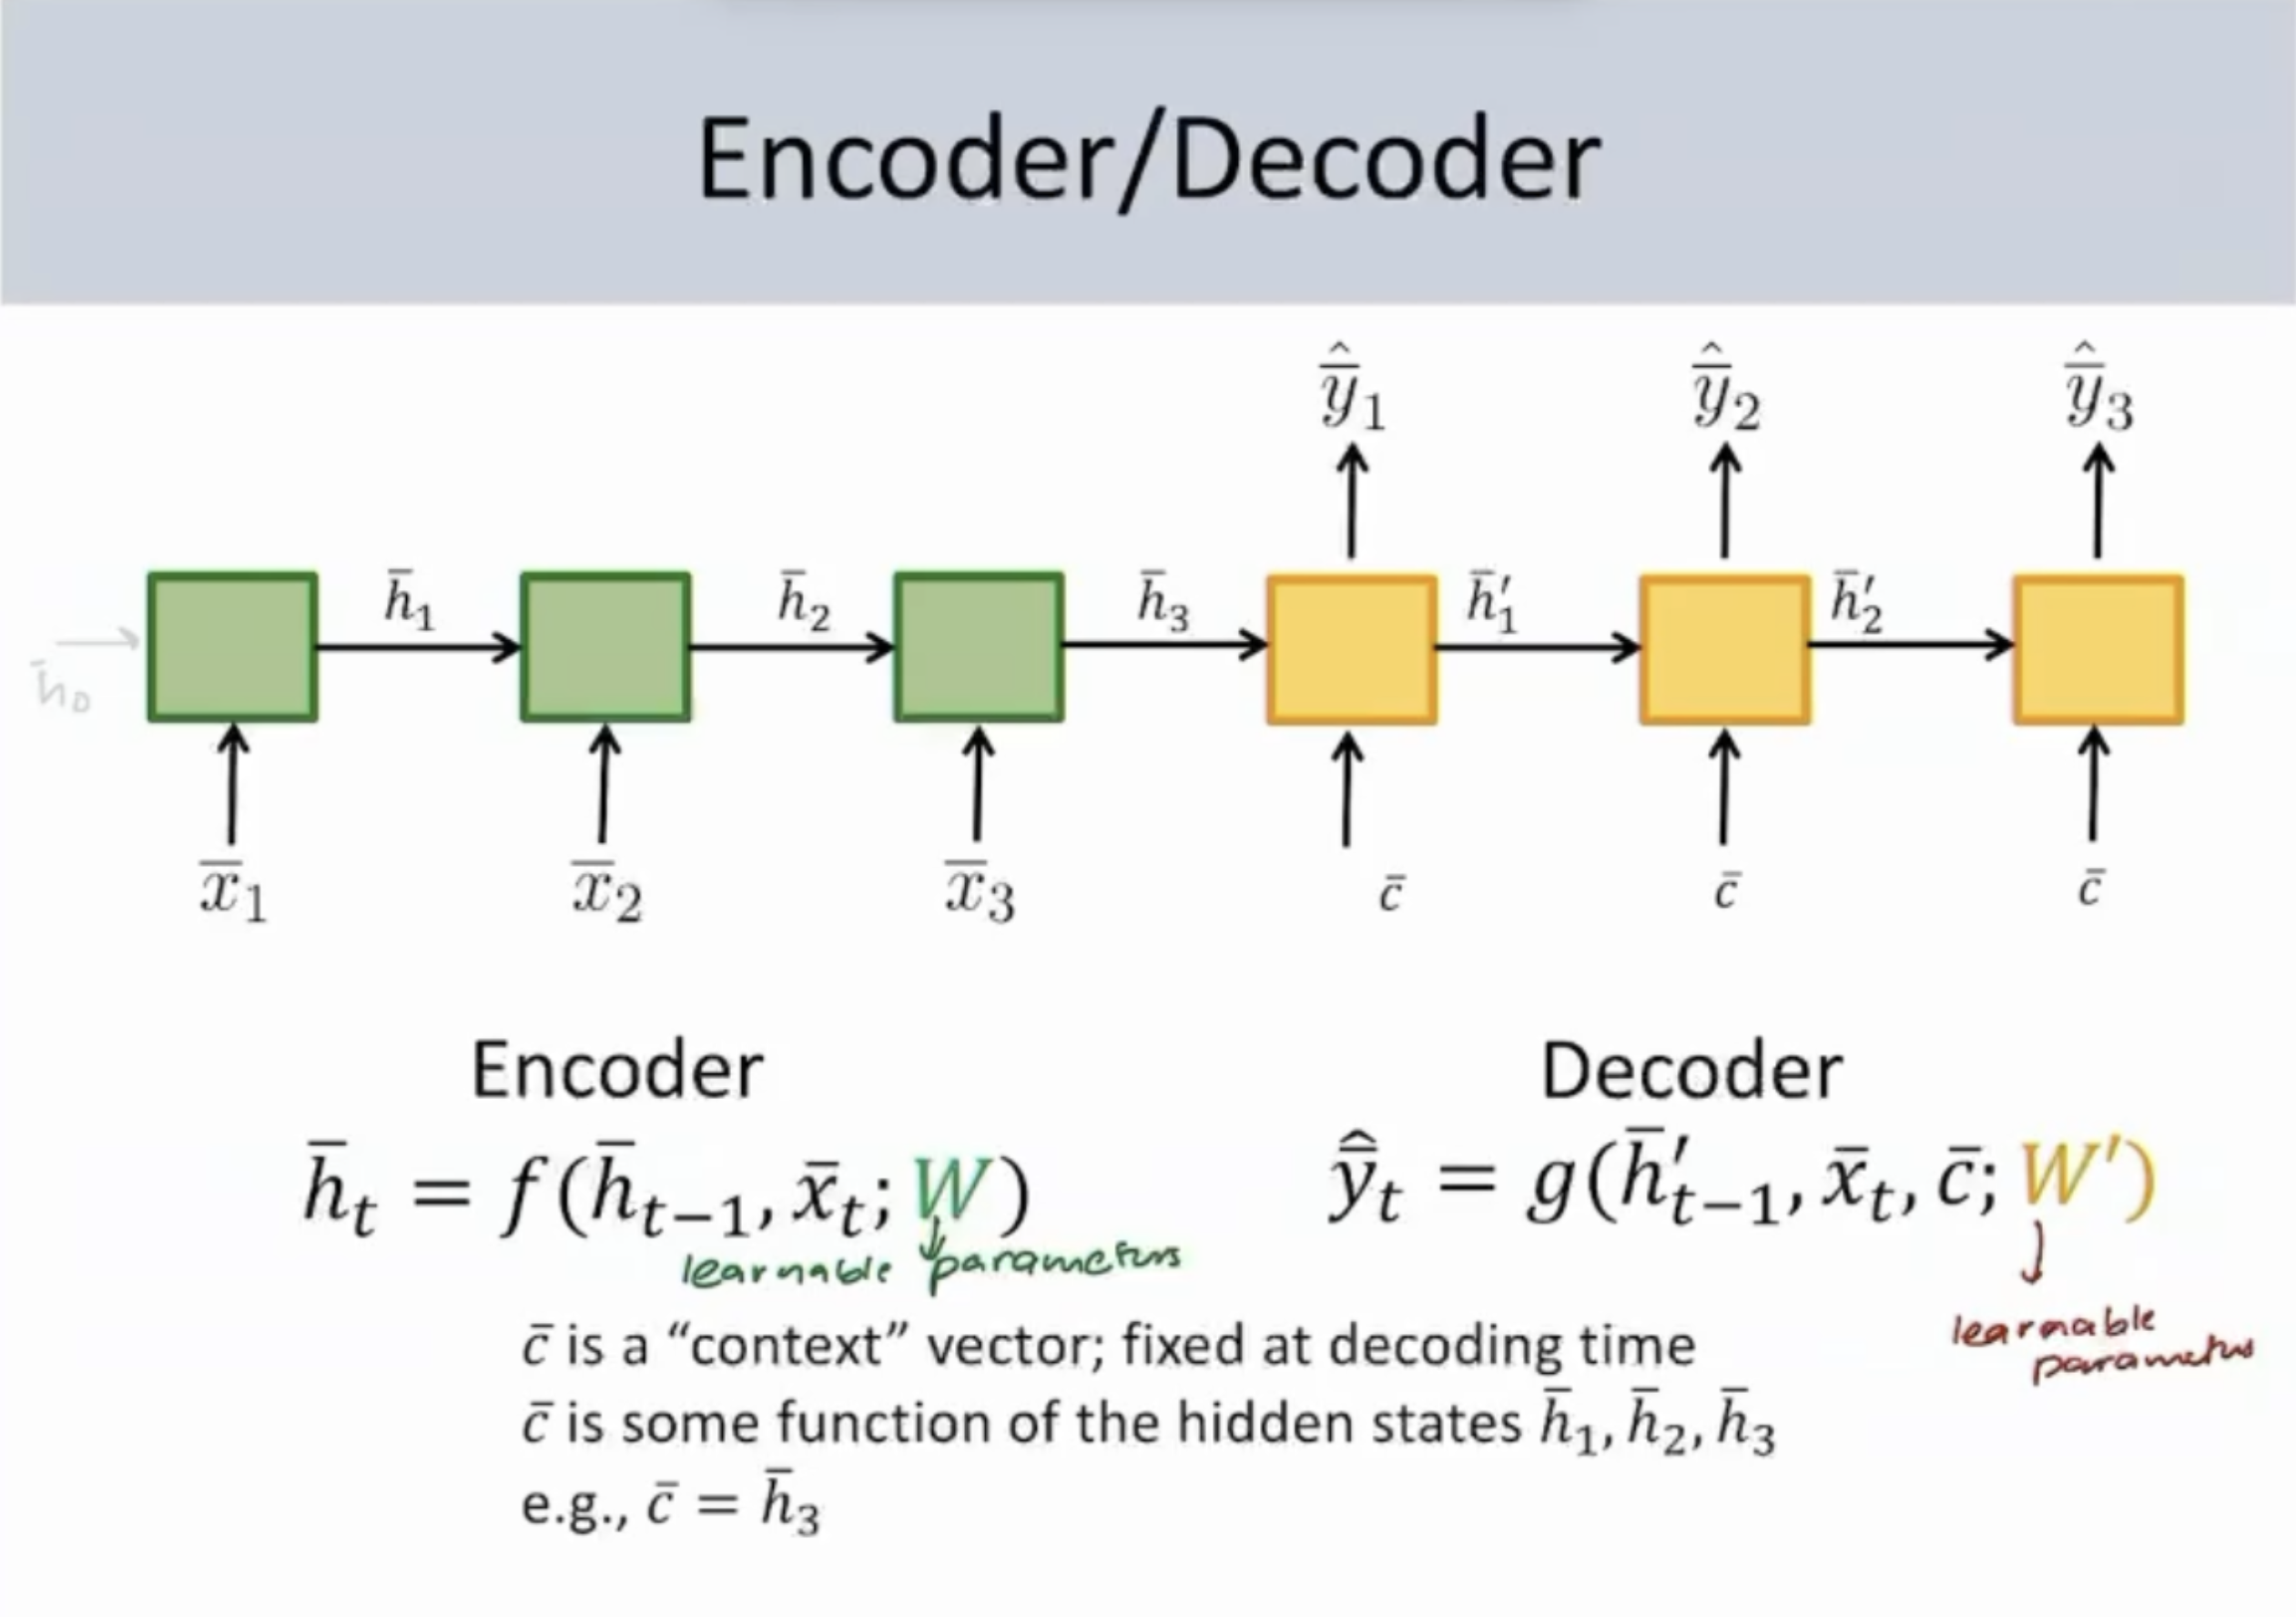
\includegraphics[width=0.75\linewidth]{images/encoder_decoder_example_1.png}

This is the original encoder/decoder architecture. As the figure states, $\bar c$ is some hidden state that is fixed at decoding time and is passed as input into each decoder block. Notice that using the same hidden state for each decoding block isn't necessary, so changing this hidden state (or in a different sense, paying attention to different hidden state) at decoding time is the first step.

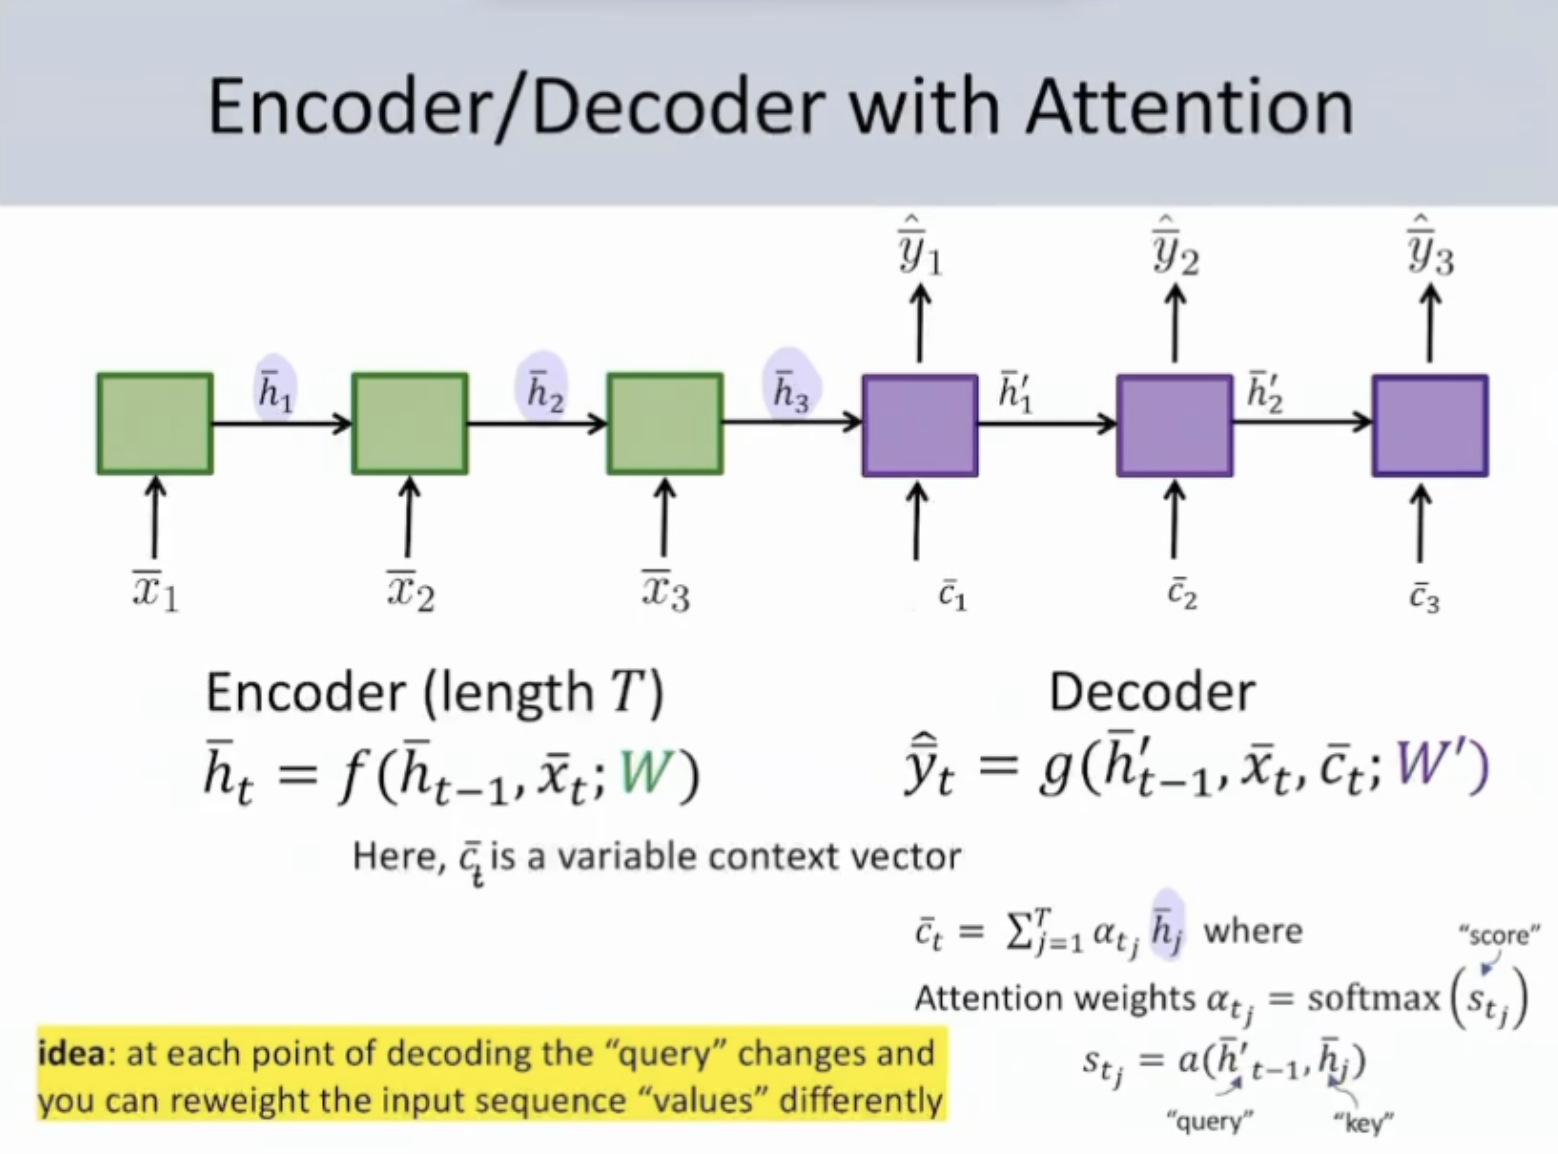
\includegraphics[width=0.75\linewidth]{images/encoder_decoder_with_attention_example_1.png}

Let $a$ be a simple dot product between the input parameters. With attention, the idea is that you change the amount of attention that you give to each of the input tokens ($\bar x_1, \bar x_2, \dots, \bar x_T$) depending on how similar the current hidden state $\bar h'_{t-1}$ in the decoder stage is to those input tokens. You can see this happening when computing $s_{tj}$, since the dot product measures similarity between two vectors. After taking the softmax of $\bar s_t$, we get the attention weights for each encoder token, which is multiplied by our encoder token vector to create our context vector $\bar c_t$. Here is an example of computing the context vector at $t=2$:

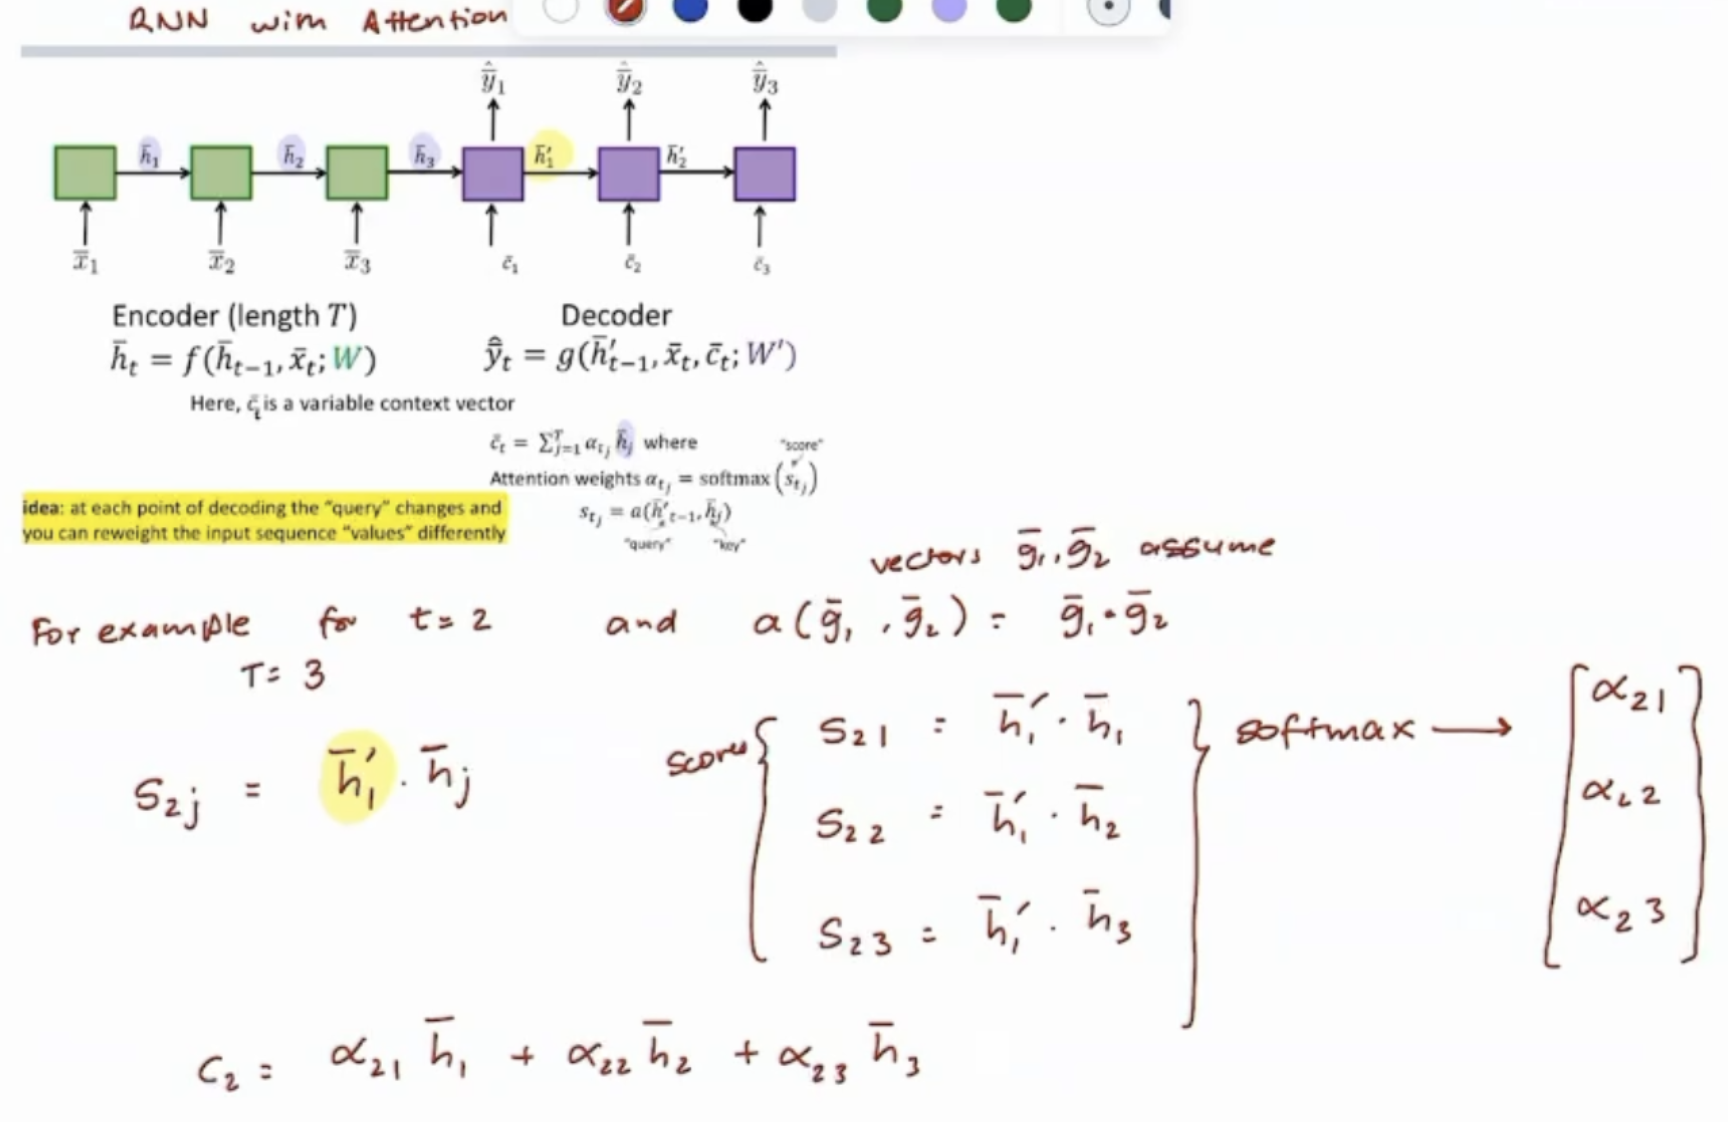
\includegraphics[width=0.75\linewidth]{images/encoder_decoder_with_attention_example_2.png}

\part{Lecture 17}

\section{Transformers: Architecture}

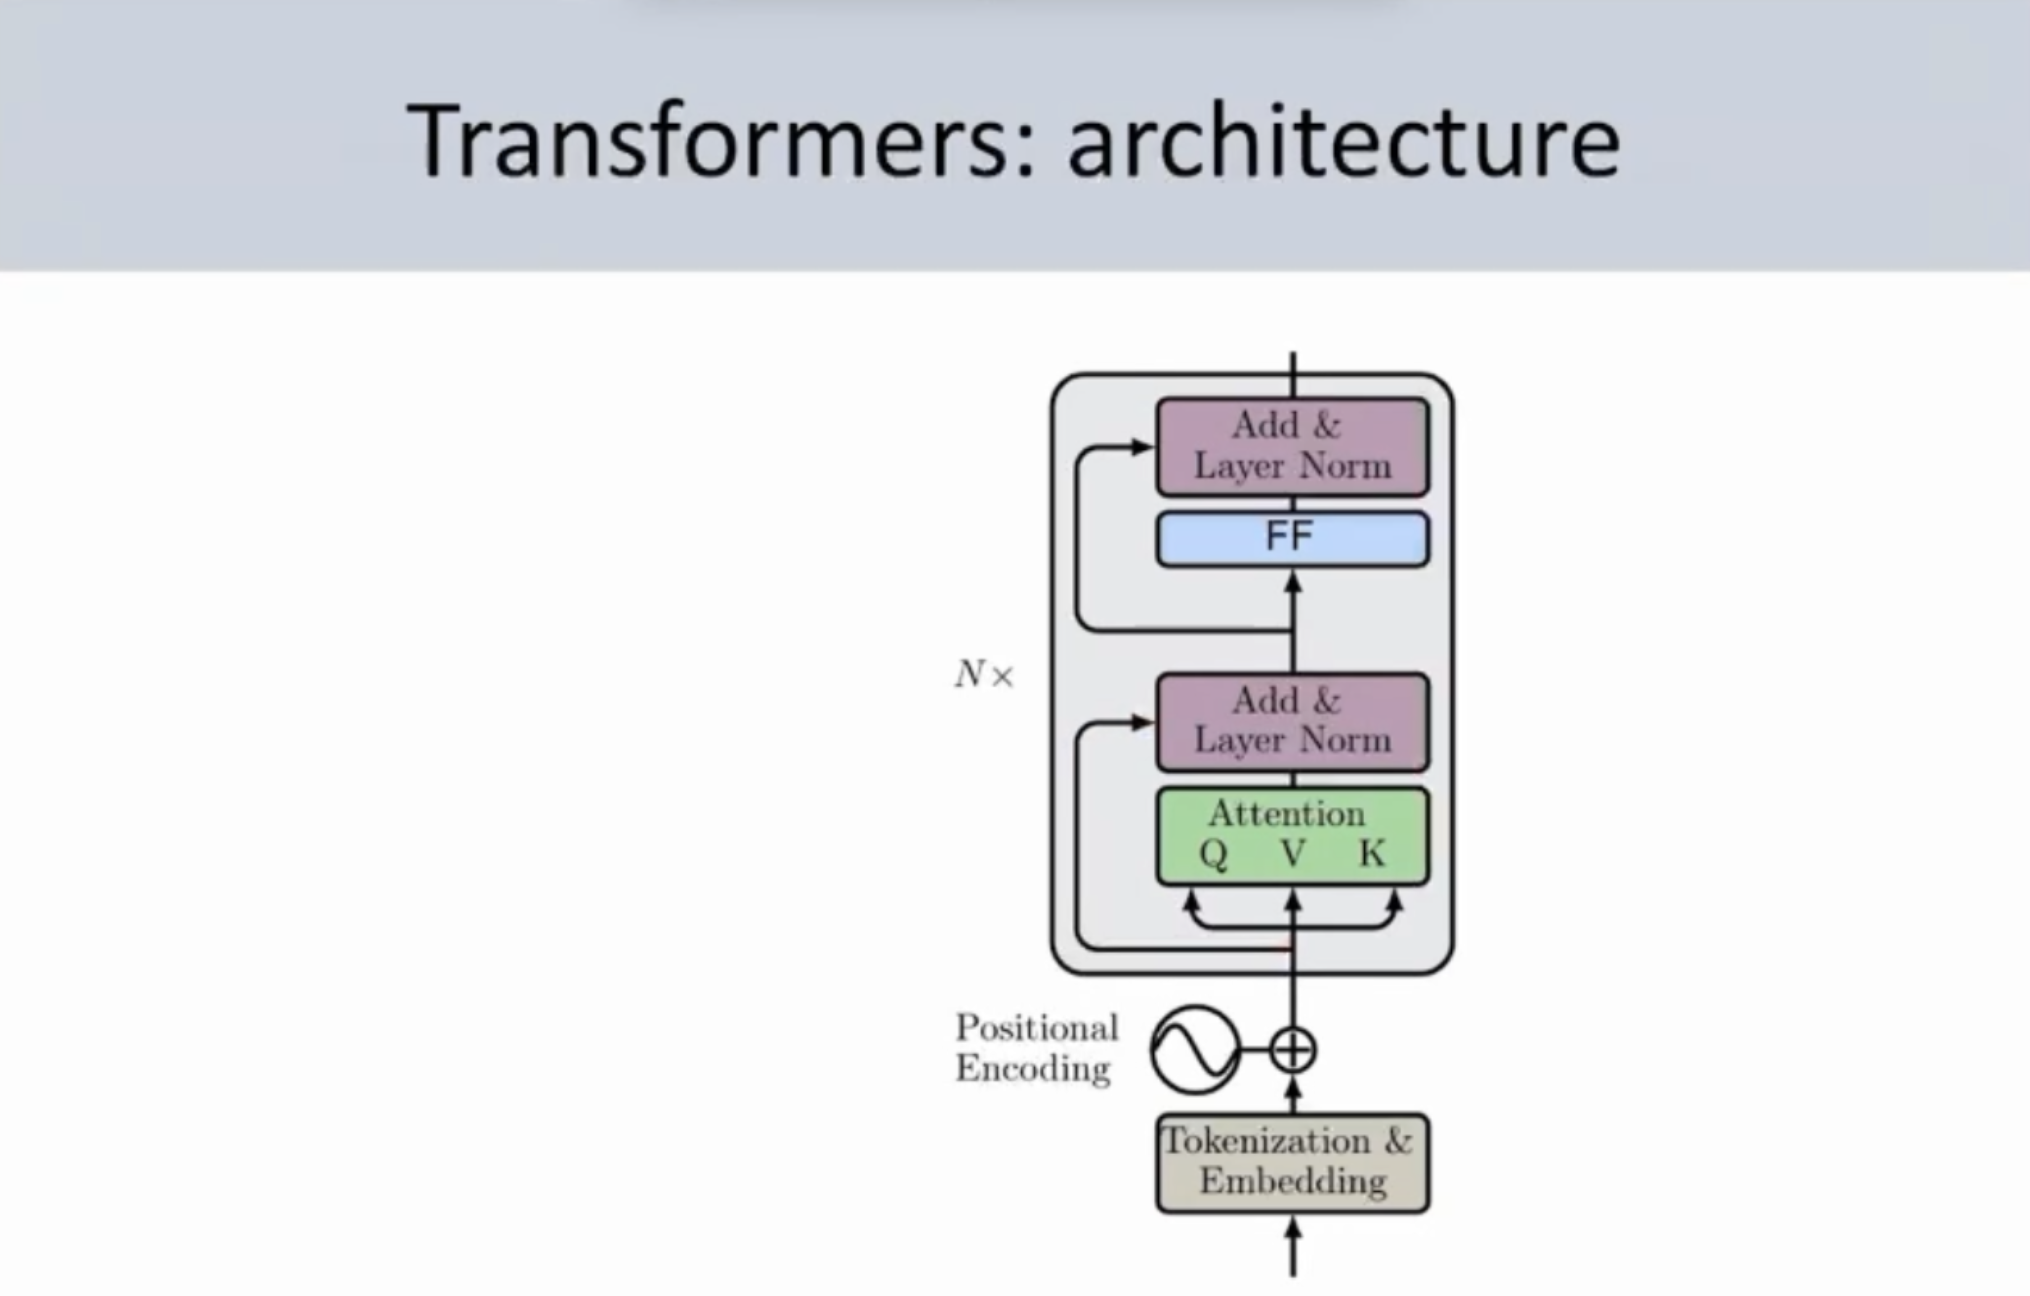
\includegraphics[width=0.75\linewidth]{images/transformers_example_1.png}

We will go through each part of this architecture one-by-one. Our focus will be in Natural Language Processing (NLP).

\subsection{Transformers: Tokenization \& Embedding}

This layer's goal is to take an input and 1. seperate the input into tokens and 2. map the tokens into Euclidean Space. The first part is called Tokenization and the second part is called Embedding. The output from this layer is a sequence of vectors, where vector $i$ corresponds to the embedded value of token $i$.

\begin{itemize}
	\item Tokenization: The idea behind tokenization is to break down raw text into smaller, manageable units called tokens. Computers can't read a string of text all at once; they need a discrete vocabulary to reference. The granularity for tokens in this class are usually entire words, but they could easily be smaller. Sub-word tokens (ex: ``unhappiness" $\rightarrow$ [``un", ``happi", ``ness"]) are nice because they allow a model to infer the meaning of a word its never seen before by looking at their pieces. Once a sentence is split into tokens, each unique token is assigned a specific ID.
	\item Embedding: The idea behind embedding is to map those raw IDs or tokens into vectors in a high-dimensional Euclidean Space. In this high-dimensional space, two close vector would signify high relations between those corresponding tokens. At the end of this embedding, we can use vector arithmetic to generate meaning. For example:
		$$\text{Vector(``King")} - \text{Vector(``Man")} + \text{Vector(``Woman")} \approx \text{Vector(``Queen")}$$
		\begin{itemize}
			\item Note: The problem with raw IDs is that they exist in $\R^1$, whereas human language is multi-dimensional. A single word has many features/meanings all at once. For example, take the word ``Apple":
				\begin{itemize}
					\item It is a Fruit (biological feature)
					\item It is Red/Green (visual feature)
					\item It is a Tech Company (corporate feature)
					\item It is Cruchy (texture feature)
				\end{itemize}
				In $\R^1$, you can only measure distance in two ways (left or right). In a high-dimensional space, the model can use some dimensions to represent food features and an entirely different dimension to represent corporate features. This allows ``Apple" to be close to ``Banana" while also being close to ``Microsoft" without creating an incomprehensible mess like it would in $\R^1$ (``Banana" would be forced to be close to ``Microsoft").
			\item Note: Obviously, this Embedding seems very complex. The ways this is done is out of scope for this class, but I really want to learn how they do this.
		\end{itemize}
\end{itemize}

\subsection{Transformers: Positional Encoding}

\textbf{Idea:} Retain information about the order of the word\\

Suppose the output from tokenization + embedding is $\bar x_1', \dots, \bar x_T'$ and positional encoding is $\bar p_1, \dots, \bar p_T$. We could simply create $\bar e_1', \dots, \bar e_T' = \bar x_1' + p_1, \dots, \bar x_T' + p_T$. Obviously this might not be the best way to encode position into our tokens, but its reasonable for now.\\

The goal of positional encoding is to create a way for the computer to distinguish between two sentences with exactly the same words but different order of words. For example, we want

\begin{center}
	``dog chased cat" \quad and \quad ``cat chased dog"
\end{center}

to look different in the computers eyes. To do this, we could serially process each word in the sequence and treat words in different sequence positions slightly differently. To parallelize this, we add preset positional information to all elements. The results looks like the following:

\[ \text{``dog"} ~ = [0, 1], \quad \text{``chased"} ~ = [1, 0], \quad \text{``cat"} ~ = [1, 1] \]
\[ \bar p_1 = [0, 0.2], \quad p_2 ~ = [0.2, 0], \quad p_3 ~ = [0.2, 0.2] \]
\[ \text{``dog chased cat"} ~ = [0, 1], [1.2,0], [1.2,1.2] \]
\[ \text{``cat chased dog"} ~ = [1, 1.2], [1.2, 0], [0.2, 1] \]


\subsection{Bidirectional self-attention} \label{bidirectional self-attention}

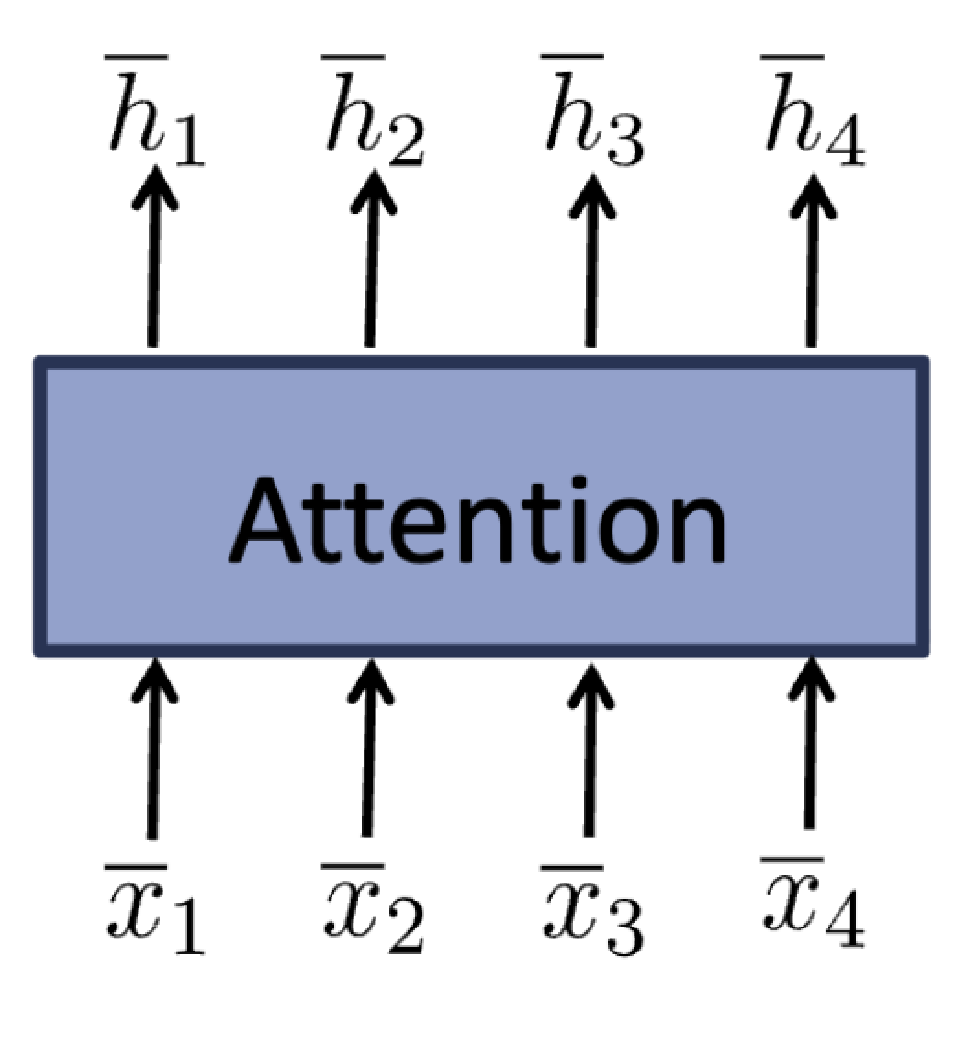
\includegraphics[width=0.5\linewidth]{images/bidirectional_self_attention_example_1.png}

\[ \bar h_i = \sum_{j=1}^T softmax(s_{ij}) \bar v_j, \quad s_{ij} = \frac {\bar k_j \cdot \bar q_i} {\sqrt{d_k}} \]

where 

\[ 
	\begin{aligned}
		\text{``query"} & \bar q_i = W^Q \bar x_i & W^Q \in \R^{d_k \times d}\\
		\text{``key"} & \bar k_j = W^K \bar x_j & W^K \in \R^{d_k \times d}\\
		\text{``value"} & \bar v_j = W^V \bar x_j & W^V \in \R^{d_V \times d}\\
	\end{aligned}
\]

\textbf{Note:} The reason we divide by $\sqrt{d_k}$ is because our representations $\bar q$ and $\bar k$ tend to be vectors of numbers around 1 on average, so if you estimate the l2 norm of $\bar k \cdot \bar q$, you would get $\sqrt{d_k}$.\\

The idea behind Bidirectional self-attention is that you want to find a representation for each token in the input sequence base on its relation with all (or some, ex causal self attention) other tokens in the input sequence. When calculating these attention weights, the model stores three types of information (query, key, and value) for each input token. Each of the three types of information has a different use:

\begin{itemize}
	\item Query: This represents the information that is important for the model to understand this specific token. 
		\begin{itemize}
			\item Role: It probes the other tokens to see which ones are relevant to its own meaning.
			\item Example: In the sentence ``The bank of the river," the Query for the word "bank" might be looking for ``nature-related context" to distinguish it from a financial institution.
		\end{itemize}
	\item Key: This acts as a label or an index that describes what kind of information that token offers.
		\begin{itemize}
			\item Role: The system calculates the Dot Product ($s_{ij} = \bar{k}_j \cdot \bar{q}_i$) between a Query and a Key to determine the ``similarity score." If the Query and Key match well, the score is high, meaning that specific token is very relevant.
			\item Example: In the same sentence, the token ``river" has a Key that says ``I am a body of water." When the Query for ``bank" hits this Key, they match, and the model pays attention to ``water" when it tries to understand ``bank"
		\end{itemize}
	\item Value: This is the actual content or ``payload" of the token. Once the model knows which tokens are important (via the Q and K match), it extracts the actual information of the tokens from the Values.
		\begin{itemize}
			\item Role: The output $\bar{h}_i$ is a weighted sum of these Values. If a Key had a high attention score, its corresponding Value will contribute heavily to the final representation of the current token.
			\item Example: If the model determines that ``river" is highly relevant to ``bank," it takes the ``water/nature" information from the Value of ``river" and adds it to the new representation of ``bank."
		\end{itemize}
\end{itemize}

You can see all of this happening in the original formula for calculating $\bar h_i$ at the beginning of this subsection. Here is a visual example of this calculation:

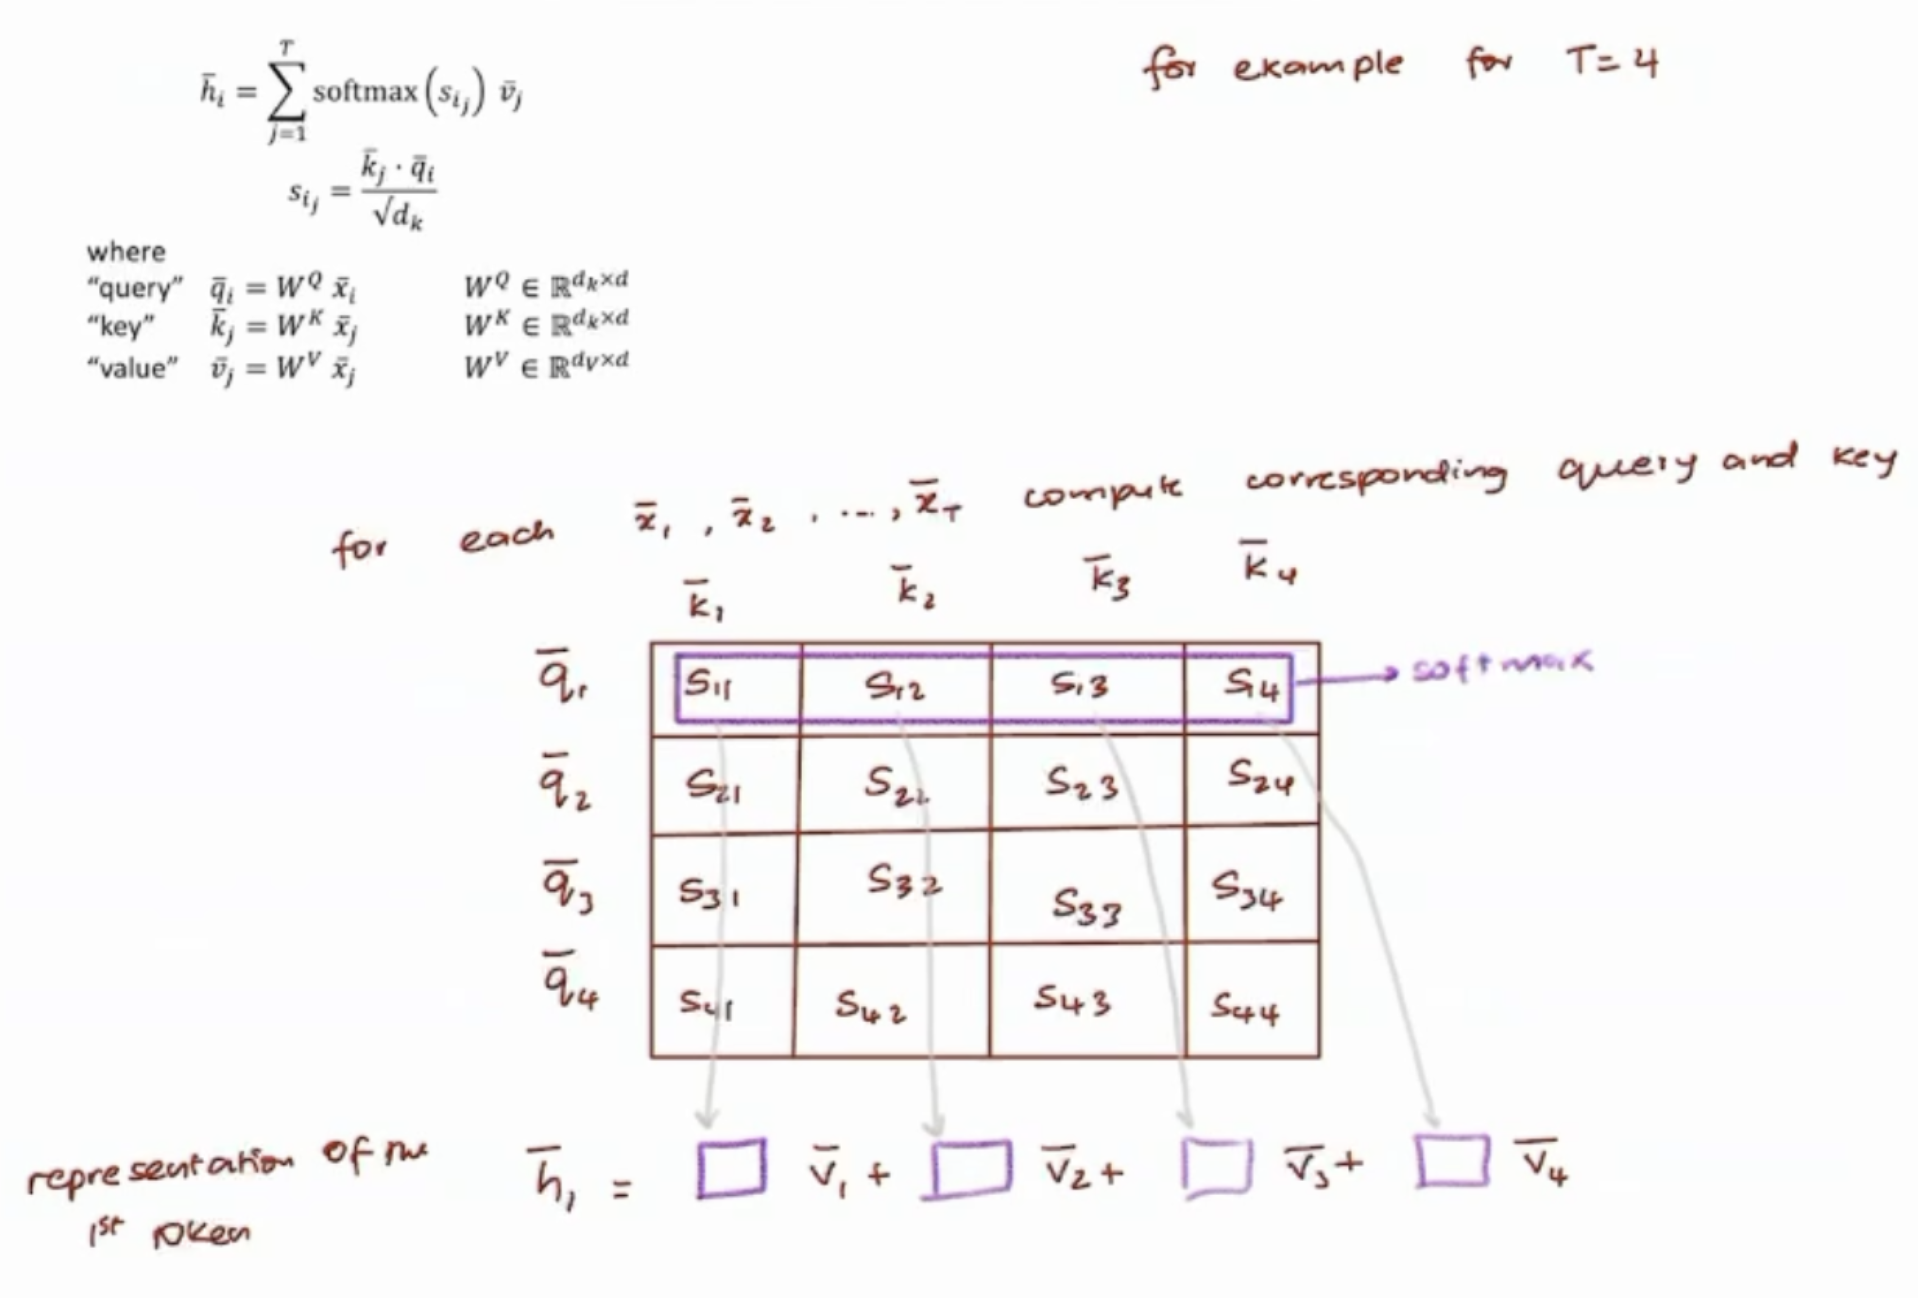
\includegraphics[width=0.75\linewidth]{images/bidirectional_self_attention_example_2.png}

\textbf{Note:} There is a lot that we don't understand fully about deep learning. All that has been said in this section is suspition as to what these representations learn. This is why it seems so arbitrary to say a specific vector represents ``queries" and another represents ``keys" when in reality the model will simply learn weights in an architecture that will result in the best performance. This is all what we think would make the most sense for the model to learn. 

\subsection{Transformers: Batch/Layer Normalization}

\begin{itemize}
	\item Batch Norm: Normalize the same features across mini-batches. Batch norm is the more intuitive way to normalize datapoints.
		\begin{itemize}
			\item Ex: 
				\begin{tabular}{|c|c|c|c|c|c|c|c|c|}
					\hline
					& $\bar x^{(1)}$ & $\bar x^{(2)}$ & $\bar x^{(3)}$ & mean & std\_dev & $\hat x^{(1)}$ & $\hat x^{(2)}$ & $\hat x^{(3)}$ \\
					\hline
					$x_1$ & 1 & 3 & 8 & 4 & 2.94 & -1.02 & -0.34 & 1.36\\
					\hline
					$x_2$ & 3 & 4 & 3 & 3.33 & 0.471 & -0.708 & 1.42 & -0.708\\
					\hline
					$x_3$ & 5 & 6 & 2 & 4.33 & 1.69 & 0.394 & 0.986 & -1.38\\
					\hline
					$x_4$ & 7 & 2 & 1 & 3.33 & 2.62 & 1.40 & -0.509 & -0.891\\
					\hline
				\end{tabular}~\\
		\end{itemize}

	\item Layer Norm: Normalize the same datapoint across all features.
		\begin{itemize}
			\item Ex: 
				\begin{tabular}{|c|c|c|c|}
					\hline
					& $\bar x^{(1)}$ & $\bar x^{(2)}$ & $\bar x^{(3)}$\\
					\hline
					$x_1$ & 1 & 3 & 8\\
					\hline
					$x_2$ & 3 & 4 & 3\\
					\hline
					$x_3$ & 5 & 6 & 2\\
					\hline
					$x_4$ & 7 & 2 & 1\\
					\hline
					mean & 4 & 3.75 & 3.50\\
					\hline
					std\_dev & 2.23 & 1.47 & 2.69\\
					\hline
				\end{tabular}~\\

				Results:

				\begin{tabular}{|c|c|c|c|}
					\hline
					& $\hat x^{(1)}$ & $\hat x^{(2)}$ & $\hat x^{(3)}$\\
					\hline
					$x_1$ & -1.35 & -0.510 & 1.67\\
					\hline
					$x_2$ & -0.448 & 0.17 & -0.186\\
					\hline
					$x_3$ & 0.448 & 1.53 & -0.558\\
					\hline
					$x_4$ & 1.35 & -1.19 & -0.929\\
					\hline
				\end{tabular}~\\
		\end{itemize}
\end{itemize}

Oftentimes, we use Layer Norm for RNN and Transformers for two specific reasons. 

\begin{enumerate}
	\item Variable lengths: I you have a batch where one setence is 5 words and another is 50, calculating a batch mean for the 40th word is impossible because most sentences don't have one.
	\item Dependency on Batch Size: Batch Norm breaks if your batch size is small (like 1 or 2). Layer Norm doesn't care about other data points; it only looks at the current one, making it much more stable for large models where we can only fit a few examples in memory at a time (batch sizes can't be large in this case).
\end{enumerate}


\subsection{Transformers: Residual Connections \& Add}

The primary role of the Residual Connection (Add layer) is to prevent the Vanishing Gradient problem. In a standard deep network, the error signal (gradient) must pass through ever weighted layer during backprop. Because this involves a long chain of multiplications, if the weights or activations are small, the signal shrinks exponentially as it travels toward the earlier layers. By the time it reaches the bottom of the model, the gradient can become so close to zero that the initial layers stop learning entirely. The Residual Connection solves this by adding the original input $x$ to the output of the sub-layer, creating the mathematical identity $F(x) + x$. When calculating the gradient for this operation, the $+x$ term provides a constant derivative of 1, ensuring that a full-strength version of the signal can bypass the complex weights and reach the earlier layers unimpeded.\\

Beyond solving technical training issues, this structure changes what the model is actually trying to learn. Instead of forcing a block to learn a complex, entire transformation from scratch, the model only needs to learn the residual—the small edit or refinement needed to improve the current representation. If a specific attention head or feed-forward layer finds that its input is already optimal, it can simply drive its internal weights toward zero. Because of the Add step, the original information ($x$) will still flow through perfectly. This makes the identity function (passing data through unchanged) the easiest state for the model to achieve, rather than a difficult mathematical target, allowing Transformers to be stacked dozens of layers deep without losing the core meaning of the tokens.

\subsection{Transformers: Feed-Forward Neural Network}

This is just a regular FFNN. You need this layer because at the end of the day, FFNN are the best at processing/classifying data. The rest of the Transformer creating representations of the input (and output) sequencesso that the FFNN has the patterns and features it needs to optimally classify. 

\section{Types of Transformers}

\subsection{Encoder-Only transformers}

\begin{itemize}
	\item Most often use in classification setting
	\item Can stack multiple layers
	\item e.g., BERT
		\begin{itemize}
			\item Bidirection Encoder Representations from Transformers
			\item Bidirectional because every learned representation depends on tokens that precede and succeed it
		\end{itemize}
\end{itemize}

\subsection{Decoder-Only Transformers}

\begin{itemize}
	\item Most often used in text generation e.g., the GPT family
	\item Uses masked (causal) attention
	\item \textbf{Causal-self attention:} allows each position in decoder to attend to all position up to and including that position (masks all values in the input that correspond to look ahead)
		\begin{itemize}
			\item i.e., does not allow looking forward in the sequence
			\item All the math for calculating $\bar h_i$ stays the same as \ref{bidirectional self-attention}, except:

				\[ 
					s_{ij} = \begin{cases}
						\frac {\bar k_j \cdot \bar q_i} {\sqrt{d_k}} & j \le i\\
						-\infty & \text{otherwise}
					\end{cases}
				\]

				which, after sending through the softmax function, zeros all vectors that come after vector $i$.
		\end{itemize}
\end{itemize}

\subsection{Encoder-decoder Transformers}

\begin{itemize}
	\item Most often used in translation and summarization e.g., T5
	\item The output sequence uses \textbf{Masked Attention}, or Causal-self attention, to understand the context of all output already generated.
	\item Uses \textbf{cross-attention}: queries come from previous output of the decoder layer and the keys and values come from the output of the encoder. This is different from self-attention, where the all the information for each hidden state are made from the tokens in the encoder.
	\item Uses \textbf{multi-head attention}: multiple layers of attention blocks, each learning/capturing different patters within a sequence. This improves tasks like language understanding and translation.
\end{itemize}

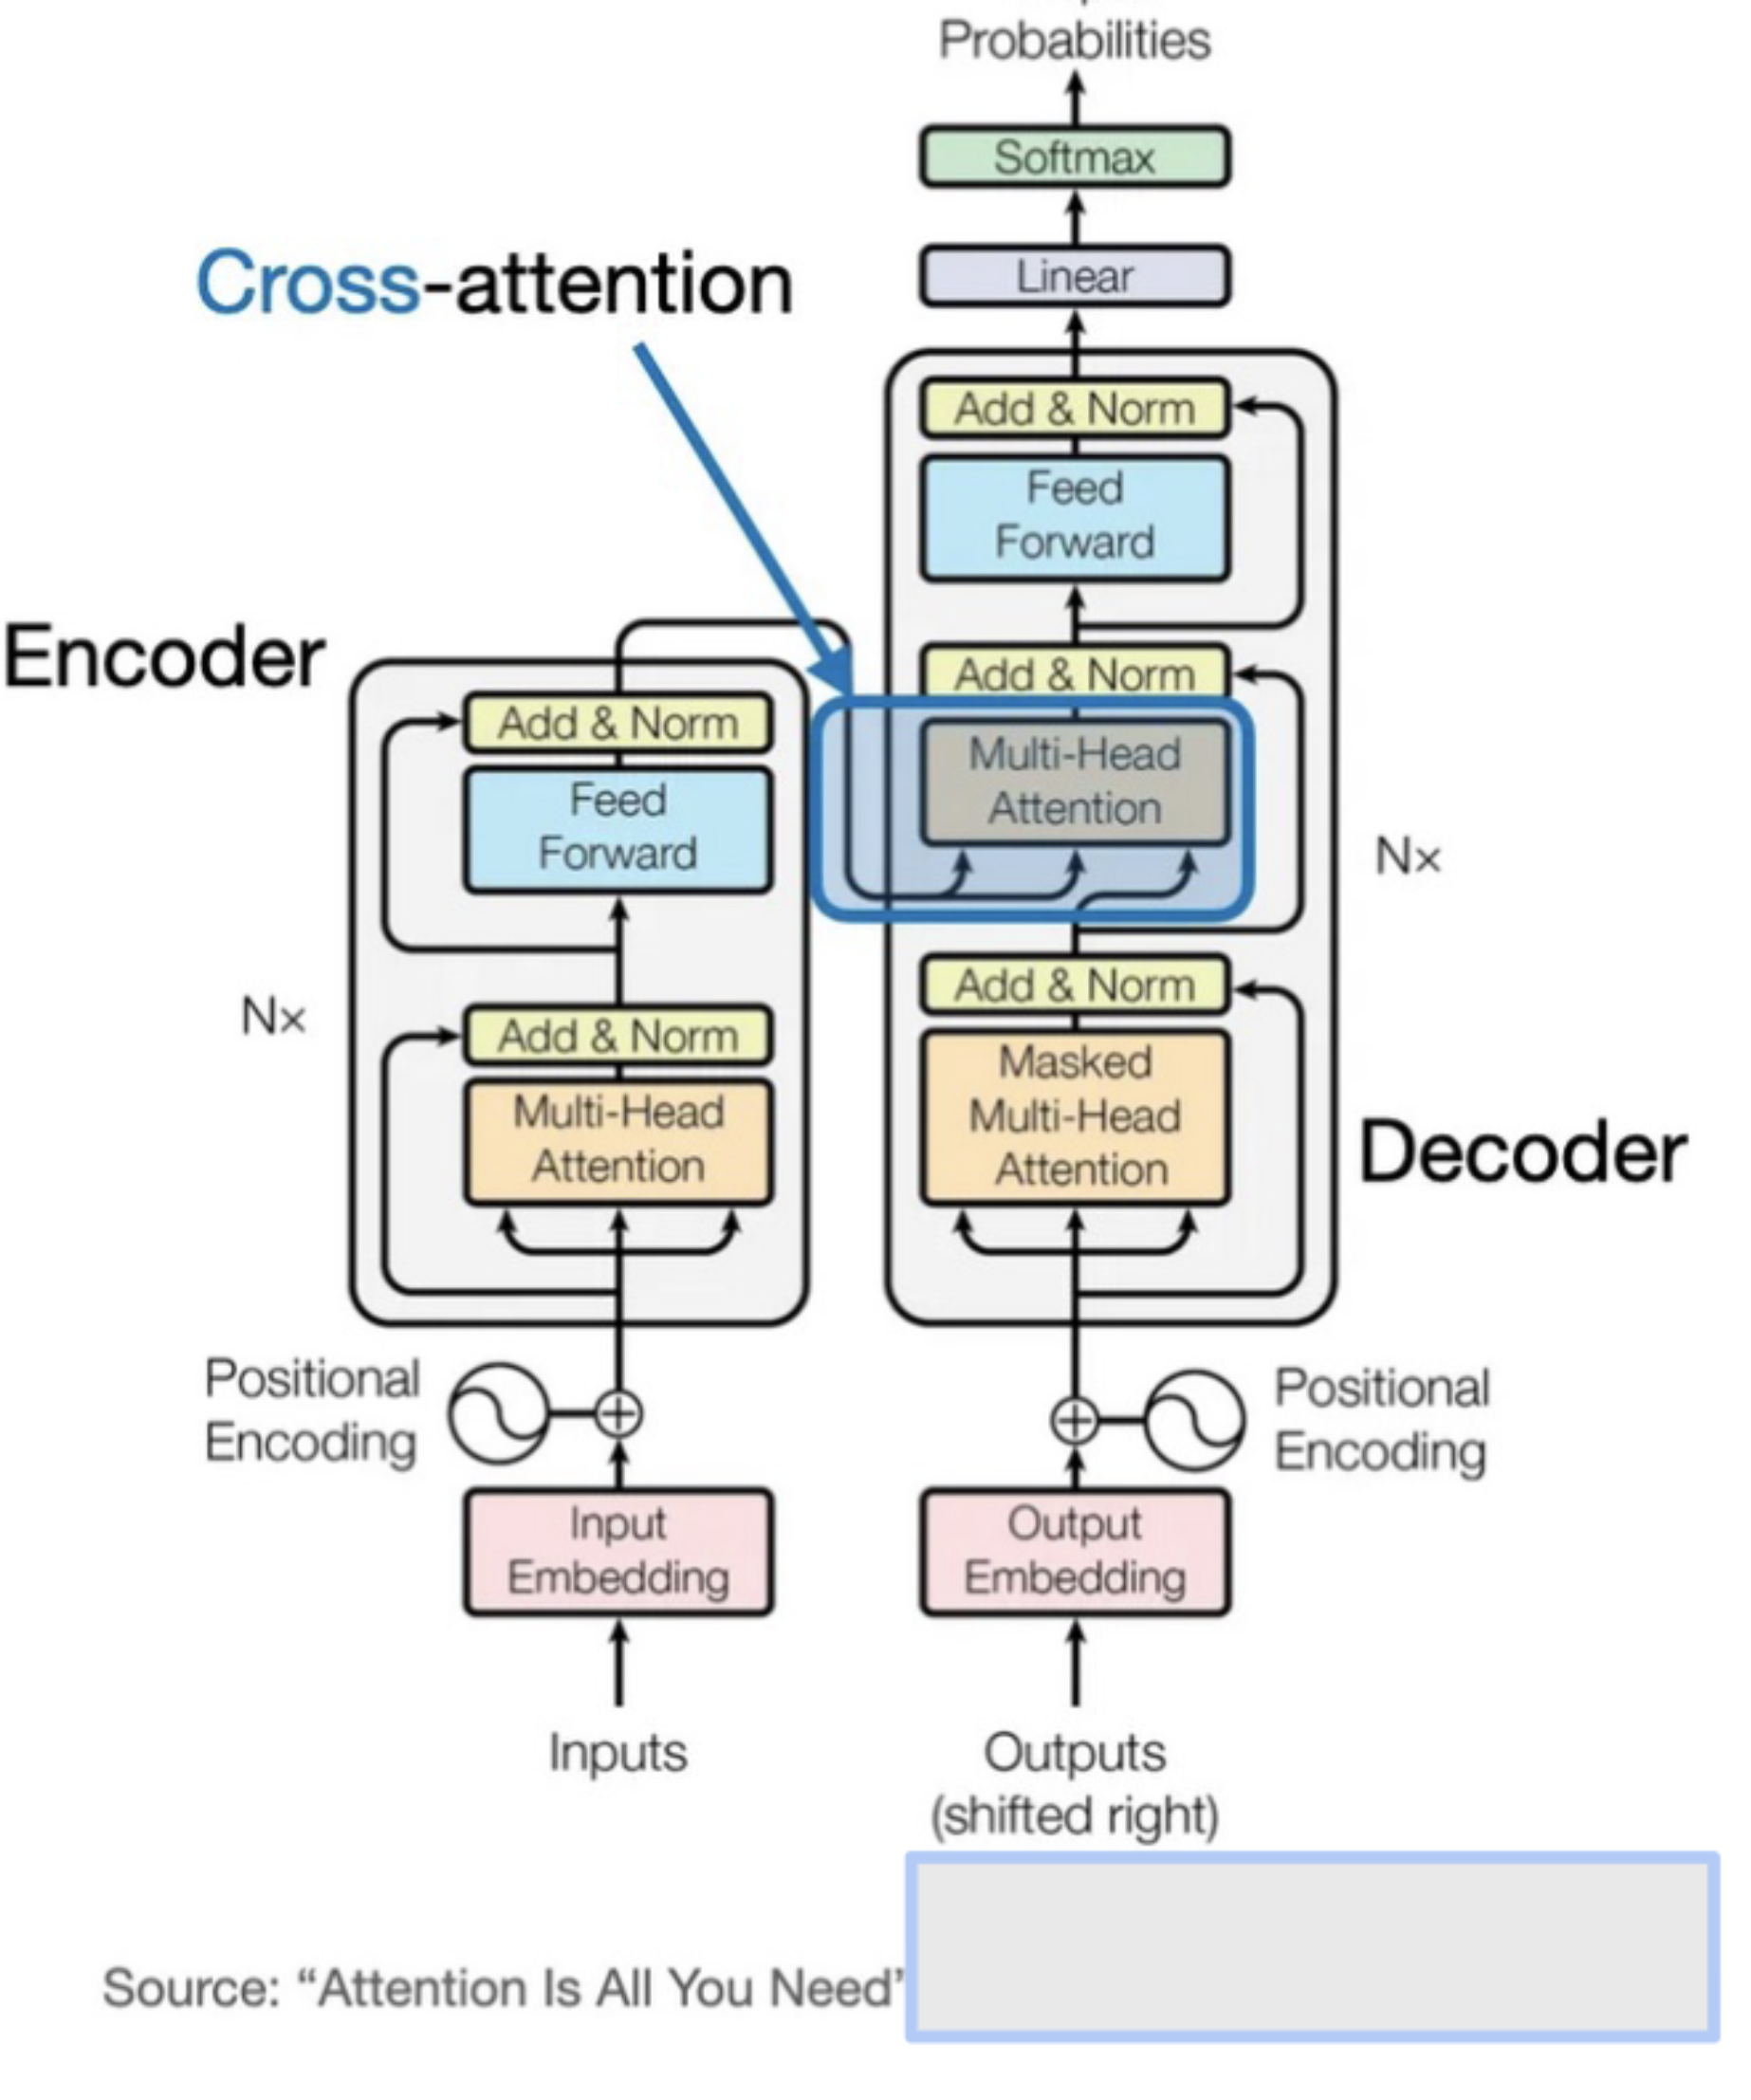
\includegraphics[width=0.75\linewidth]{images/types_of_transformers_example_1.png}

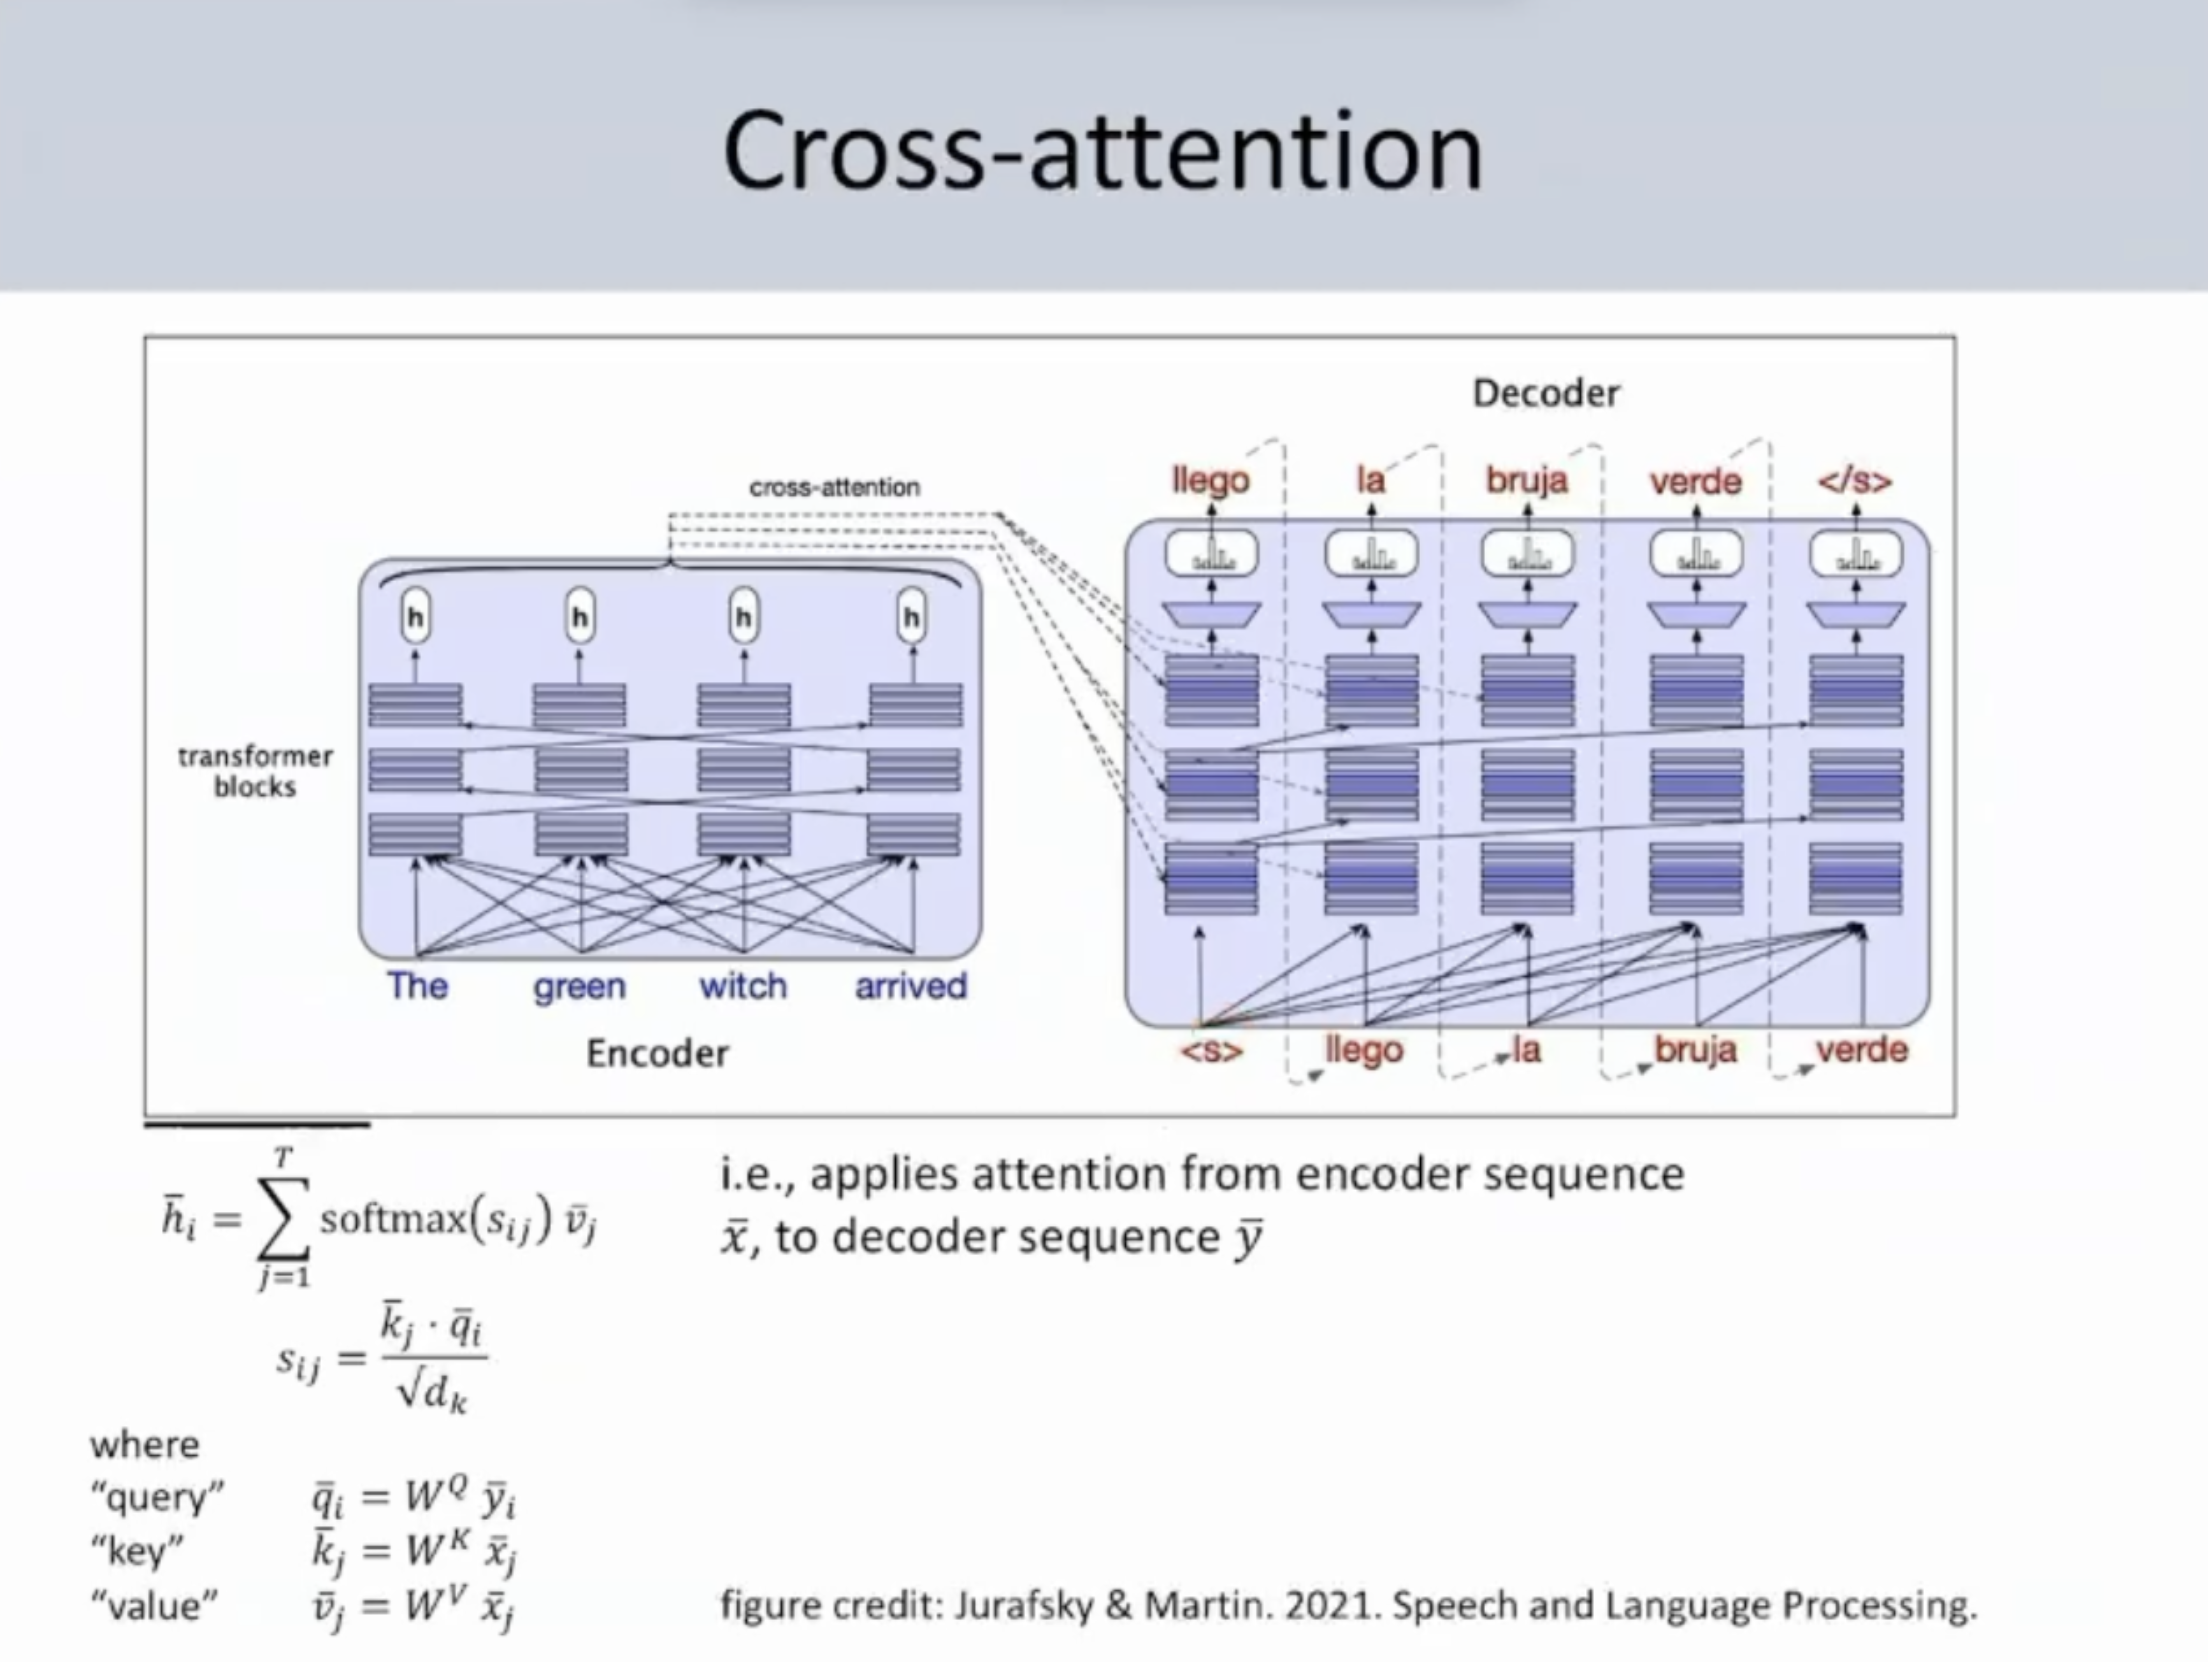
\includegraphics[width=0.75\linewidth]{images/types_of_transformers_example_2.png}

Here is a diagram of Multi-head attention:

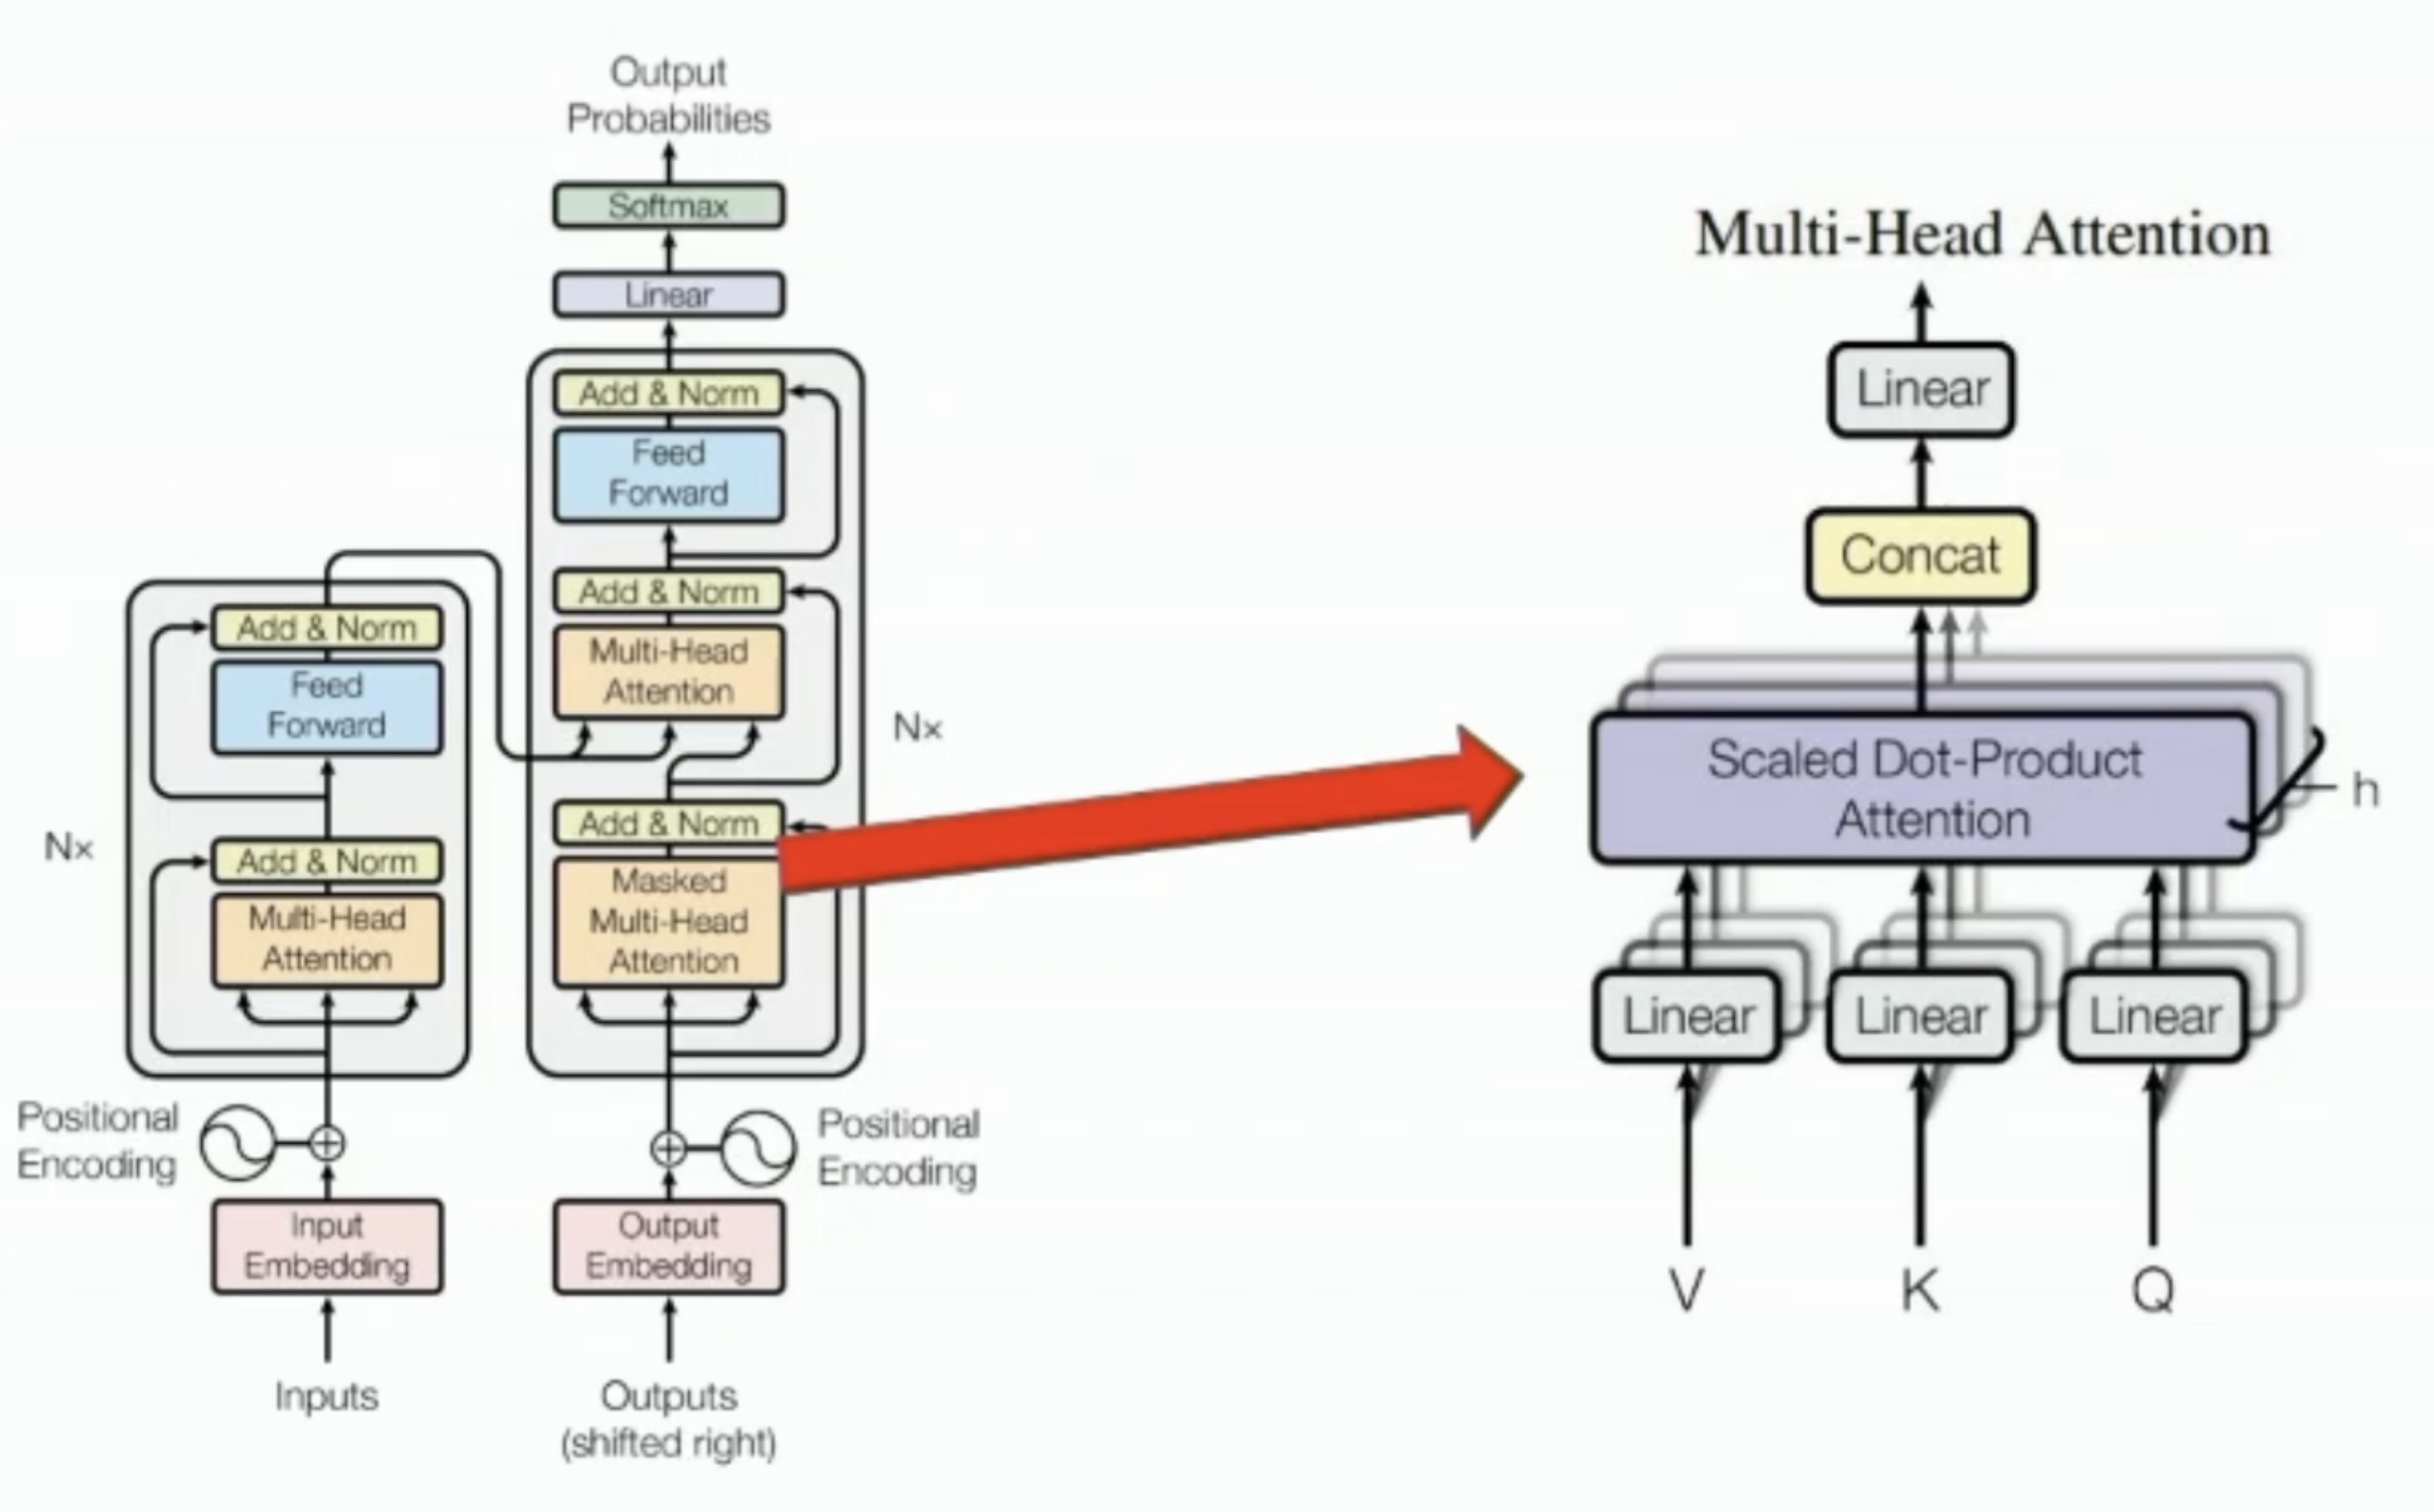
\includegraphics[width=0.75\linewidth]{images/types_of_transformers_example_3.png}

\section{Unsupervised Learning}

Up until this point, we have only talked about datasets in the following form:

\[ S_n = \{ \bar x^{(i)}, y^{(i)} \}_{i=1}^n \]

But what if we aren't given the labels $\bar y$? In this case, rather than finding patterns between similarly labeled datapoints, our goal is to generalize datapoints and see if we can make artificial groupings/patters of similar dataponts. One main question we will ask is ``where do labels come from"? Here are some options:

\begin{itemize}
	\item Domain experts (doctors, researchers, PhDs)
	\item MTurk (crowdsourcing)
	\item Generate automatically
\end{itemize}

The remainder of the class will focus on unsupervised learning and techniques to cluster similar datapoints toogether.

\part{Lecture 18}

\section{Clustering}

\textbf{Input:} $S_n = \{ \bar x^{(i)} \}_{i=1}^n \quad \bar x^{(i)} \in \R^d \quad k \text{ (number of clusters)}$\\
\textbf{Output:} a set of cluster assignements $c_1, \dots, c_n$ with each $c_i \in \{ 1, \dots, k \}$\\
\textbf{Goal:} assign similar (dissimilar) points to the same (different) cluster(s)\\

Clusters can be described by their corresponding set of examples or a representative point:

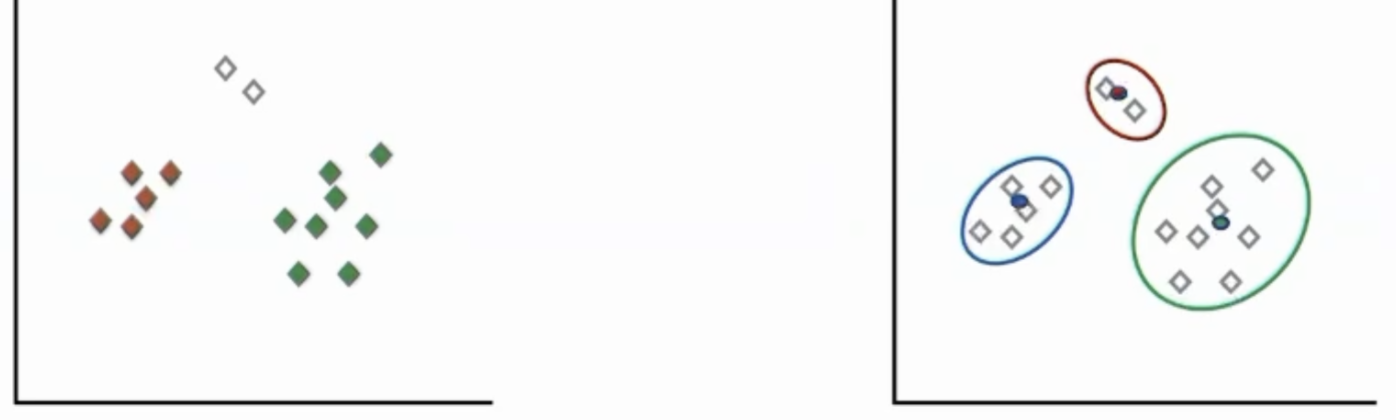
\includegraphics[width=0.75\linewidth]{images/clustering_example_1.png}

\subsection{$k$-means clustering}

\textbf{Goal:} Partition data into $k$ clusters (defined by $k$ ``means"") such that the sum of squares of Euclidean distances of each point to its cluster's mean is minimized.\\

\textbf{Steps:}

\begin{enumerate}
	\item Initialize all datapoints
	\item Randomly assign $k$ means to the Euclidean space. 
	\item Assign each datapoint to its closest mean. 
	\item Recompute the $k$ means to the mean of their assigned cluster in step (3)
	\item repeat steps 3-4 until clusters stop changing.
\end{enumerate}

Here is a visual example of how the algorithm would work:

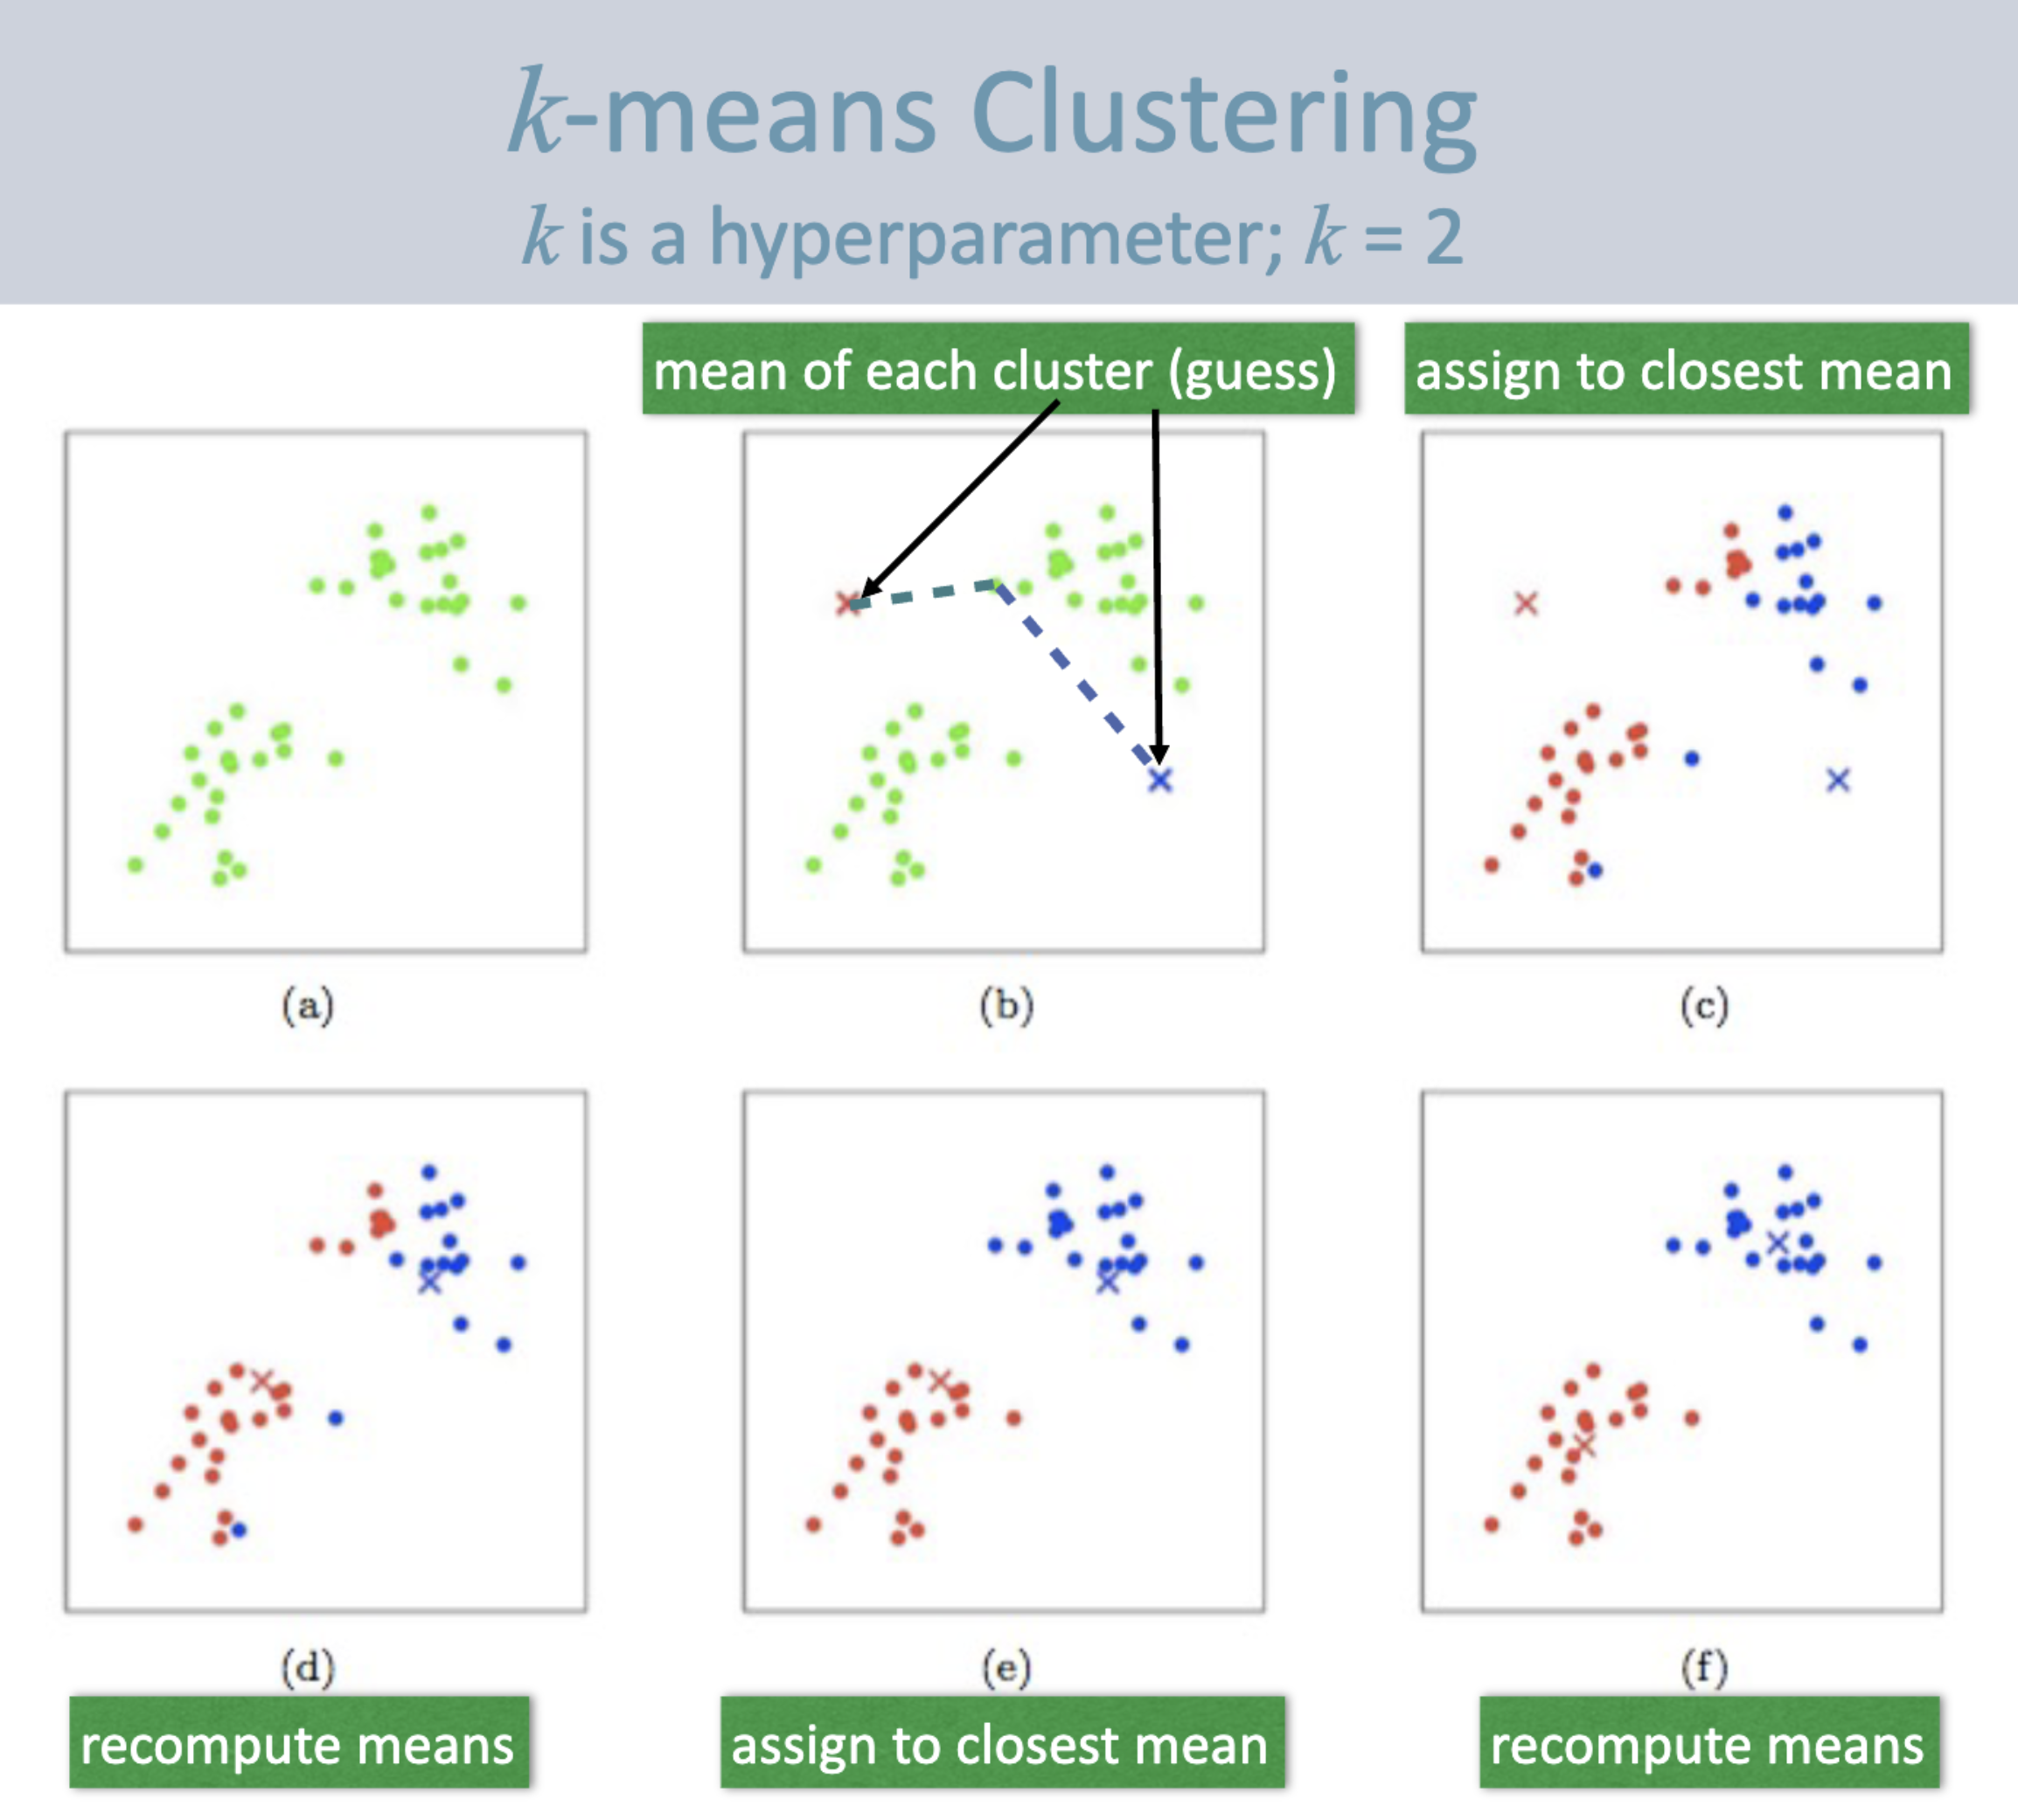
\includegraphics[width=0.5\linewidth]{images/clustering_example_2.png}

\subsection{$k$-means objective function}

For datapoints 

\[ \bar x^{(1)}, \dots, \bar x^{(n)} \]

we want to find a cluster 

\[ c_1, \dots, c_n \quad \text{with each} \quad c_i \in \{ 1, \dots, k \} \]

for each datapoint and a corresponding mean

\[ \bar {\mu}^{(1)}, \dots, \bar {\mu}^{(k)} \]

for each cluster to minimize for the objective function

\begin{equation}
	J(\bar c, M) = \sum_{i=1}^n ||\bar x^{(i)} - \bar{\mu}^{(c_i)}||^2.
	\label{eq:k-means objective function}
\end{equation}


Observe what minimizing this objective function searches for. It searches for the $\bar {\mu}^{(i)}$ for each cluster and $c_i$ for each point such that the total squared distance between all datapoints and their corresponding cluster mean is minimized. Intuitively, this seems optimal.\\

\textbf{Note:} Since $J$ must monotonically decrease, and there are a finite number of cluster assignments, $J$ must eventually converge. However, $J$ is not convex, meaning this algorithm is not guaranteed to converge to a global minimum.

\subsection{How to pick $k$-means and find global optimum efficiently}

\begin{enumerate}
	\item Option 1: Solve an $NP$-hard problem
	\item Option 2: Randonly pick amongst given datapoints (or random points in space) $\rightarrow$ works sometimes, othertimes converges to only local minimums
	\item Option 3: $k$-means++. Similar to option 2, but pick points w.r.t. already selected means. Points that further from already selected means have a higher chance of being picked. Notice that we don't automatically choose the furthest points - we still choose with randomness but weighted towards further points.
		\begin{itemize}
			\item Approximation Guarantee: The expected value of the objective returned by $k$-means is never more than O(log $k$) from optimal and can be as close as O(1) from optimal. Even in the former case, with $2k$ random restarts, one restart will be O(1) from optimal (with high probability).
		\end{itemize}
\end{enumerate}

\subsection{$k$-means clustering algorithm}

\begin{algorithm} \label{alg:k-means clustering}
	\caption{$k$-means clustering}
	\begin{algorithmic}
		\For{$i = 1, \dots, k$}
			\State assign unique $\bar {\mu}^{(i)} \in \R^d$ (see subsection 31.3)
		\EndFor
		\While{cluster assignments are non-static}
			\For{$i = 1, \dots, n$}
				\State $c_i = \underset{j \in \{ 1, \dots, k \}}{argmin}||\bar x^{(i)} - \bar{\mu}^{(j)}||^2$
			\EndFor
			\For{$j = 1, \dots, k$}
				\State $\bar{\mu}^{(j)} = \frac{\sum_i [[c_i = j]]\bar x^{(i)}} {\sum_i[[c_j = j]]}$
			\EndFor
		\EndWhile
	\end{algorithmic}
\end{algorithm}

\part{Lecture 19}

\subsection{How do we select $k$?}

Imagine we were given the following dataset:

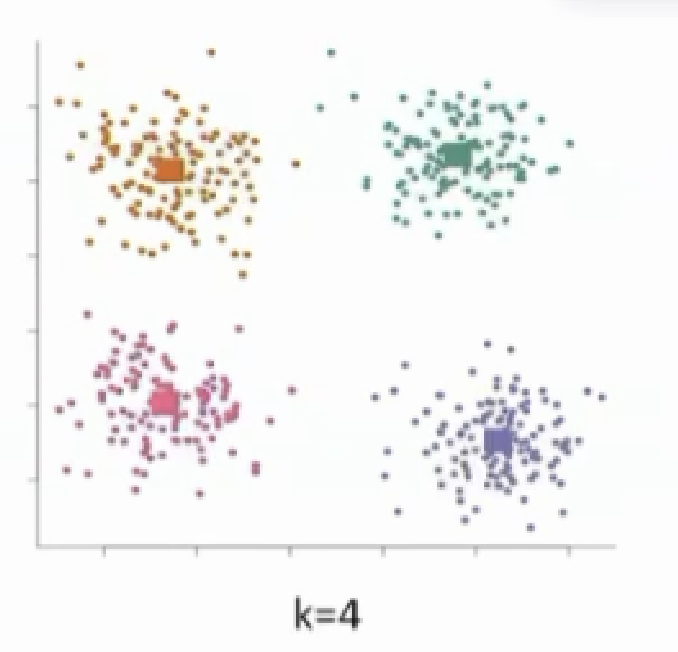
\includegraphics[width=0.5\linewidth]{images/clustering_example_3.png}

$k = 4$ clusters already seems quite satisfying. What if we chose a higher $k$? What would the cluster means look like then? It turns out, the cluster means don't converge to particularly satisfying solutions. In fact, higher $k$ values simply break up the given clusters into smaller clusters, which doesn't seem like should be the case. 

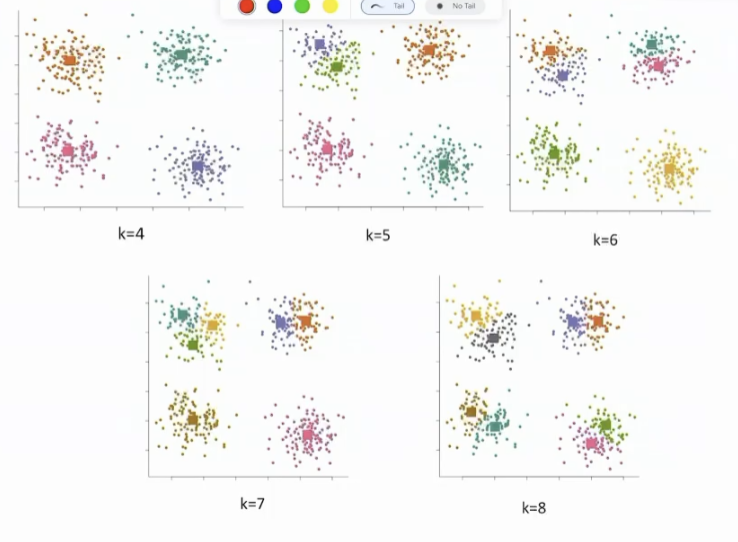
\includegraphics[width=0.5\linewidth]{images/clustering_example_4.png}

However, higher $k$ values will always lead to lower value for our objective function $J$. In fact, the value $k = n$ can easily lead to a $J = 0$, since each datapoint would be in a cluster of their own. So, it doesn't seem reasonable to choose $k$ that results in the minimum $J$.\\

A heuristic that works generally well is the \textbf{Elbow method}. This method exploits the tendancy that if datapoints are distributed in a globby way such that $k$-means is a very appropriate algorithm for the question, you will see an elbow-like shape in the objective function plotted againset $k$:

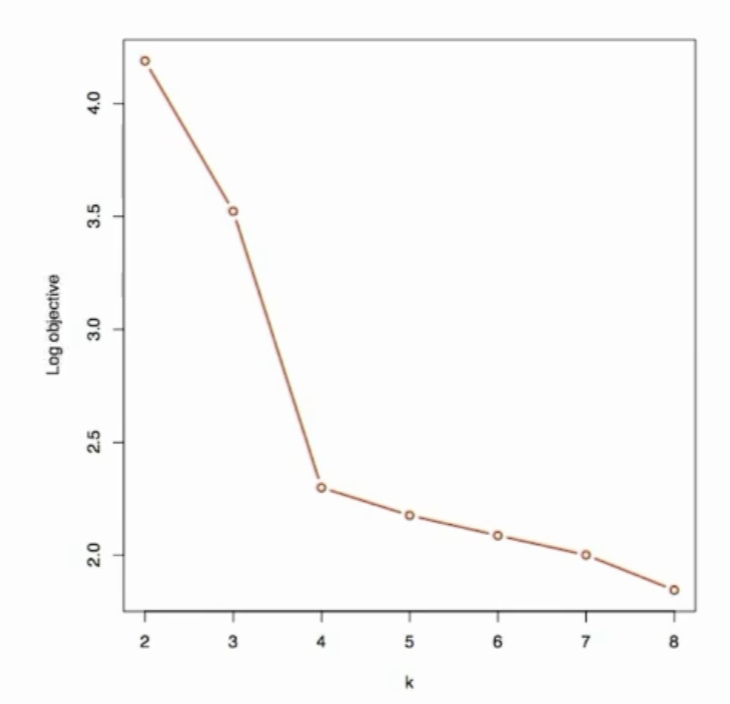
\includegraphics[width=0.5\linewidth]{images/clustering_example_5.png}

After the big drop and the relatively small drops afterwards, we guess that $k = 4$ is the correct number of clusters for this dataset.\\

\textbf{Note:} We talked last lecture about $J$ not being convex, and ways to become more confident that our $k$-means are at a global minimum. Applying that here, to generate the graph above, we would initialize our $k$-means using $k$-means++ and run the algorithm to convergence $2k$ times to produce each point for each individual value of $k$, and use the result that produced the minimum objective function for that $k$.

\subsection{$k$-means clustering claims}

\begin{enumerate}
	\item $k$-means performs \textbf{coordinate descent} on the objective function $J$ from equation (\ref{eq:k-means objective function})
	\item $k$-means is guaranteed to converge, though not guaranteed at the global minimum. This is because coordinate descent is a greedy algorithm that decreases the objective function at each step, and $J$ is not a convex function. Thus, coordinate descent can get stuck at local optimums.
	\item $k$-means++ Approximation Guarantee: The expected value of the objective returned by $k$-means is never more than O(log $k$) from optimal and can be as close as O(1) from optimal. Even in the former case, with $2k$ random restarts, one restart will be O(1) from optimal (with high probability).
\end{enumerate}

\subsection{When $k$-means doesn't work well}

Here is an example dataset and what we want $k = 3$ clusters to converge to:

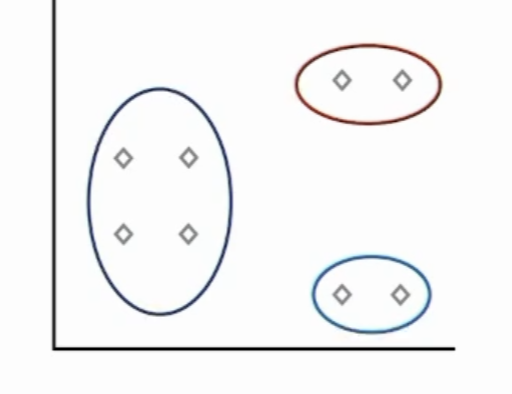
\includegraphics[width=0.5\linewidth]{images/clustering_example_6.png}

However, this isn't always what the algorithm will converge to. One other possible convergence, for a different initilization of the $k$ means, is this:

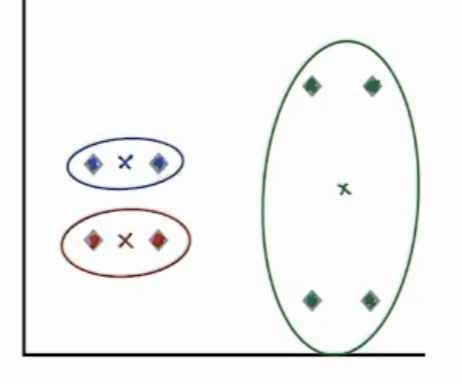
\includegraphics[width=0.5\linewidth]{images/clustering_example_7.png}

Obviously, in this case, $k$-means++ initialization would essentially guarantee a solution for the global minimum, since a very small proportion of initialization will actually end up in the bad convergence case. However, in other cases, we might not be so lucky. For example, for the following datasets, we want

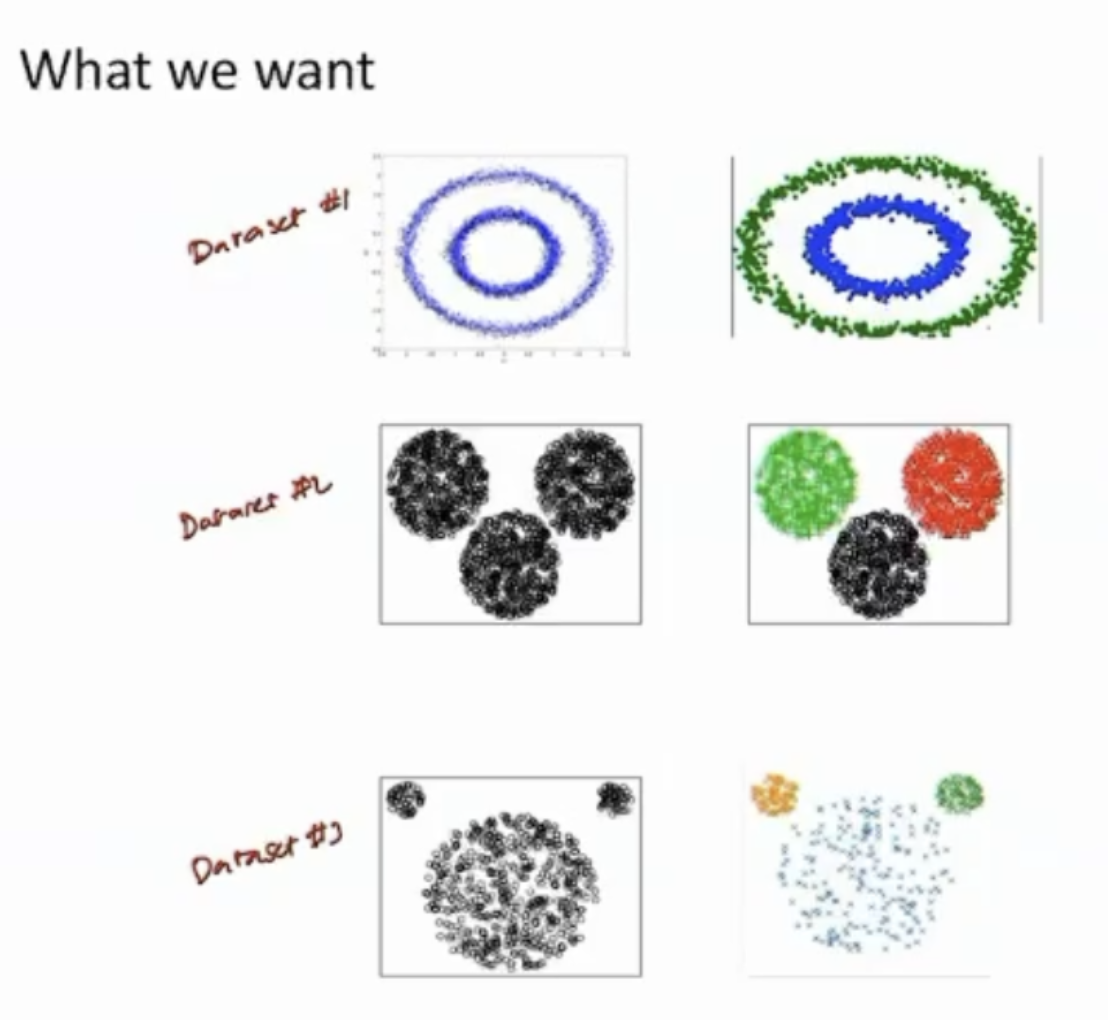
\includegraphics[width=0.5\linewidth]{images/clustering_example_8.png}

but from our current $k$-means algorithm, we would get:

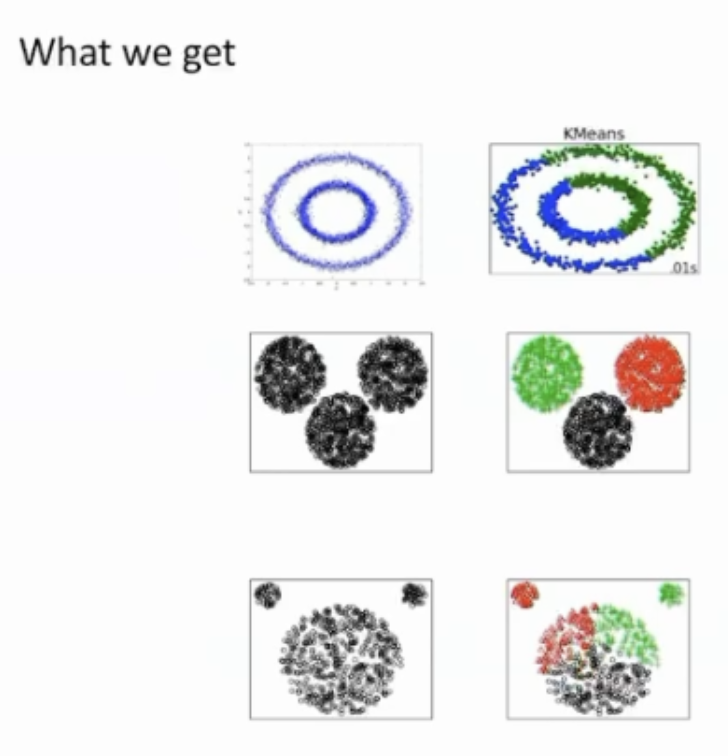
\includegraphics[width=0.5\linewidth]{images/clustering_example_9.png}

To solve the first dataset, we would need to raise our dataset to a higher dimension using a feature map, or the kernel trick. The second dataset is already a perfect problem for $k$-means due to its evenly sized clusters. The third dataset need a more genearlized algorithm (namely, the EM algorithm in subsection \ref{sub:33.4}) to acheive our preferred clusters.

\section{Discriminative vs Generative Models}

So far in the class, we have only talked about discriminative models, which have a sole goal of creating a decision boundary to guess labels based on patterns in the source dataset. Generative models are a way for us to understand where our data comes from. We can do this by using probability distributions to make some guess about the underlying probability distribution that created our data. 

\subsection{Why do we care about a generative story?}

\textbf{Better understanding of where our data came from; how it was generated}

\begin{itemize}
	\item describes internal structure of the data
	\item can also be used for classification
	\item We can use this as a basis for soft clustering
	\item We can use this as a basis for graphical models
\end{itemize}

All of this is extremely important \emph{especially} in the context of unsupervised learning. Having an understanding of the distribution of datapoints is essentially what we were doing with the $k$-means clustering algorithm and can become very important in our goals of generating guesses for labels.

\subsection{Probability Rules}

\textbf{Product Rule:} $p(X,Y) = p(X | Y) p(Y) = p(Y | X) p(X)$\\
\textbf{Sum Rule:} $p(X) = \sum_Y p(X,Y) = \sum_Y p(X|Y)p(Y)$

\subsection{Maximum Likelihood Estimation (MLE)}

Given 

\[ S_n = \{ \bar x^{(i)} \}_{i=1}^n \]

assume

\begin{itemize}
	\item each $\bar x^{(i)} \sim \mathcal{D}$ \hfill (identically distributed)
	\item $\forall i \ne j \quad p(\bar x^{(i)}, \bar x^{(j)}) = p(\bar x^{(i)}) p(\bar x^{(j)})$ \hfill (independently distributed)
\end{itemize}

Consequently

\[ p(S_n) = \prod_{i=1}^n p(\bar x^{(i)}) \]

\textbf{Goal: }Determine $\mathcal{D}$. We typically assume that $\mathcal{D}$ is from some family of (parameterized) distributions so that the problem is now to estimate the parameters.\\

In other words, the goal of MLE is to find the probability distribution that maximizes the likelihood of producing given dataset. This is slightly different from finding the most likely distribution (MAP) given the dataset for the following reasosn. Firstly, the MLE maximizes for

\[ P(\text{Data} | \theta) \]

whereas MAP maximizes for

\[ P(\theta| \text{Data}) = \frac {P(\text{Data}|\theta) P(\theta)} {P(\text{Data})}. \]

Notice for the MAP calculation, if the prior ($\bar{\theta}$) is uniform, then maximizing for MLE equivalently maximizes for MAP.\\


\textbf{Note:} Observe that maximizing for MAP does not require $P(\text{Data})$ to be calculated, since this is a constant value that doesn't change where the peak of the function is.


\part{Lecture 20}

We will be going over 4 main scenarios in this lecture:

\begin{enumerate}
	\item MLE for $x^{(i)} \in \R$ generated using a univariate Gaussian
	\item MLE for $\bar x^{(i)} \in \R^d$ generated using a multivariate Gaussian
	\item Spherical Gaussian
	\item Mixture of Distribution (EM algorithm)
\end{enumerate}

\subsection{Univariate Gaussian (normal) Distribution}

We assume each datapoint $x^{(i)} \in \R$ is generated i.i.d. from an unknown Gaussian distribution. In other words, each datapoint was drawn from the same ``bell curve".\\

Each Gaussian distribution $\mathcal{N}$ is parameterized by two values, the mean $\mu$ and the varaince $\sigma^2$.\\

The Probability Density function for the Gaussian is

\[ \mathcal{N}(x | \mu, \sigma^2) = \frac 1 {\sqrt{2 \pi \sigma^2}} \exp \left(- \frac {(x - \mu)^2} {2 \sigma^2}\right) \]

\subsection{MLE for univariabel Gaussian}

Given $S_n = \{ x^{(i)} \}_{i=1}^n$ with $x^{(i)} \in \R$ drawn iid from the Gaussian, we have

\[ p(S_n) = \prod_{i=1}^n \mathcal{N}(x^{(i)}| \mu, \sigma^2). \]

Our goal for MLE is to maximize $p(S_n)$. Essentially, we are finding the highest likely probability distribution that would have resulted in our given dataset. Since we are given all $x^{(i)}$ from our dataset $S_n$, we need to find the parameters of the Gaussian $\mu$ and $\sigma^2$. So our goal is to 

\begin{itemize}
	\item Maximize $p(S_n)$ wrt $\mu$
	\item Maximize $p(S_n)$ wrt $\sigma^2$
\end{itemize}

Maximizing this function directly is really hard since we have a product of many Gaussian terms. If we instead optimized for the log likelihood of $p(S_n)$, then the product becomes an addition. Optimizing for the log likelihood turns out to also optimize for the original likelihood because the log function is a strictly monotonically increasing function. The log likelihood function is 

\[ 
	\begin{aligned}
		l(S_n; \mu, \sigma^2) &= \ln \left[ \prod_{i=1}^n \mathcal{N}(x^{(i)}| \mu, \sigma^2) \right]\\
													&= \sum_{i=1}^n \ln \left[ \mathcal{N}(x^{(i)}| \mu, \sigma^2) \right]\\
													&= \sum_{i=1}^n \ln \left[ \frac 1 {\sqrt{2 \pi \sigma^2}} \exp \left(- \frac {(x^{(i)} - \mu)^2} {2 \sigma^2}\right) \right]\\
													&= \sum_{i=1}^n \ln \left[ \frac 1 {\sqrt{2 \pi \sigma^2}} \right] + \ln \left[ \exp \left(- \frac {(x^{(i)} - \mu)^2} {2 \sigma^2}\right) \right]\\
													&= \sum_{i=1}^n \ln \left[ \frac 1 {\sqrt{2 \pi \sigma^2}} \right] - \frac {(x^{(i)} - \mu)^2} {2 \sigma^2}\\
													&= n\ln \left[ \frac 1 {\sqrt{2 \pi \sigma^2}} \right] - \frac 1 {2 \sigma^2} \sum_{i=1}^n (x^{(i)} - \mu)^2\\
													&= -\frac n 2 \ln (2 \pi \sigma^2) - \frac 1 {2 \sigma^2} \sum_{i=1}^n (x^{(i)} - \mu)^2\\
	\end{aligned}
\]

\begin{itemize}
	\item Maximize $l(S_n; \mu, \sigma^2)$ wrt $\mu$:
		\[ 
			\begin{aligned}
				\frac {dl(S_n; \mu, \sigma^2)}{d\mu} &= 0\\
																						 &= -\frac 1 {2 \sigma^2} \sum_{i=1}^n 2(x^{(i)} - \mu)(-1)\\
																						 &= \frac 1 {\sigma^2} \sum_{i=1}^n x^{(i)} - \mu\\
																						 &= -\frac {n \mu} {\sigma^2} + \frac 1 {\sigma^2} \sum_{i=1}^n x^{(i)}\\
			\end{aligned}
		\]

		So

		\[ \mu_{MLE} = \sum_{i=1}^n \frac {x^{(i)}} n \]

	\item Maximize $l(S_n; \mu, \sigma^2)$ wrt $\sigma^2$
		\[ 
			\begin{aligned}
				\frac {dl(S_n; \mu, \sigma^2)}{d\sigma^2} &= 0\\
																									&= -\frac {2n \pi} {2 \pi \sigma^2}  + \frac 2 {2 \sigma^4} \sum_{i=1}^n (x^{(i)} - \mu)^2\\
																									&= -\frac n {\sigma^2} + \frac 1 {\sigma^4} \sum_{i=1}^n (x^{(i)} - \mu)^2\\
			\end{aligned}
		\]

		So

		\[ \sigma_{MLE}^2 = \sum_{i=1}^n \frac {(x^{(i)} - \mu_{MLE})^2} n \]
\end{itemize}

\subsection{Multivariate Gaussian Distribution}

Now, $\bar x^{(i)} \in \R^d$. We have 

\[ \bar {\mu} = E[\bar x] \in \R^d \]

and our $\Sigma \in \R^{d \times d}$ (where $\Sigma_{ij}$ measures the covariance between $x_i$ and $x_j$) becomes

\[ \Sigma = E[(\bar x - \bar {\mu})(\bar x - \bar {\mu})^T]. \]

Our PDF now becomes

\[ \mathcal{N}(\bar x|\bar{\mu}, \Sigma) = \frac 1 {(2 \pi)^{d/2} |\Sigma|^{1/2}} \exp\left[ -\frac 1 2 (\bar x - \bar{\mu})^T \Sigma^{-1} (\bar x - \bar{\mu}) \right] \]

Depending on what values $\Sigma$ takes, here is a visualization of the contour plots that the Multivariate Gaussian produces:

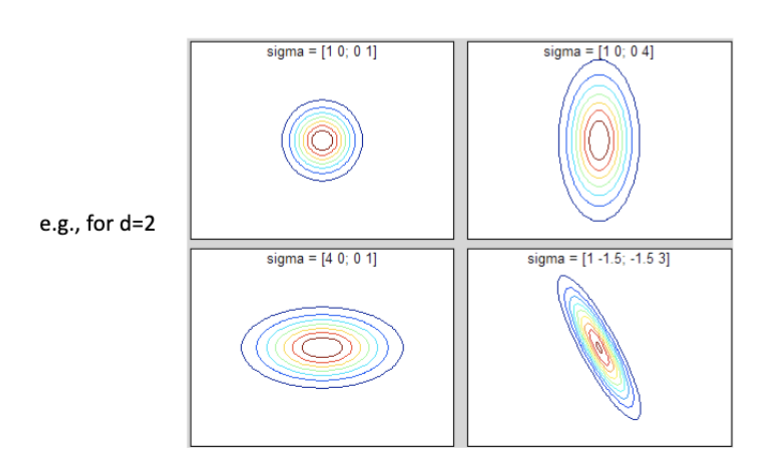
\includegraphics[width=0.5\linewidth]{images/gaussian_example_1.png}


\subsection{Spherical Gaussian Distribution}

The Spherical Gaussian is almost exactly the same as the Multivariate Gaussian, except for one thing: 

\[ \Sigma = \sigma^2 I_d \]

So $\Sigma$ only has one free parameter $\sigma$ and it is multiplied by the identity matrix (a square matrix where entries on the main diagonal are 1 and all other entries are 0). Geometrically, a spherical Gaussian model differs from a regular multivariate Gaussian model with the shape it creates. A spherical model only learns a center and a radius, creating a perfect circle or hypersphere (and contour plots with only circles/hyperspheres). A general spherical Gaussian learns covariance between dimensions, which means that divergence from the mean in one dimension lead to divergence from the mean in a correlated dimension. This leads to oval or ellipsoid shapes. We end up with the PDF:

\[ \mathcal{N}(\bar x|\bar{\mu}, \sigma^2) = \frac 1 {(2 \pi \sigma^2)^{d/2}} \exp\left[ -\frac 1 {2 \sigma^2} ||\bar x - \bar{\mu}||^2\right] \]

Now, going back to MLE, we do the following:\\

Given $S_n = \{ \bar x^{(i)} \}_{i=1}^n$ drawn iid according to $\mathcal{N}(\bar x | \bar{\mu}, \sigma^2)$, we want to maximize $p(S_n)$ wrt parameters $\bar {\theta} = (\bar{\mu}, \sigma^2)$

\[ p(S_n) = \prod_{i=1}^n p(\bar x^{(i)}) = \prod_{i=1}^n \left[\frac 1 {(2 \pi \sigma^2)^{d/2}} \exp\left( -\frac 1 {2 \sigma^2} ||\bar x - \bar{\mu}||^2\right)\right] \]

Doing this is horribly complex. We would have to calculate the partial derivative wrt $\bar {\mu}$ the partial derivative wrt $\sigma^2$, which sounds terrible in this amount of products in this equation. Instead of optimizing for the raw likelihood, we will optimize for the log likelihood.

\subsection{Log Likelihood of the Spherical Gaussian}

\[ 
	\begin{aligned}
		l(S_n; \bar{\mu}, \sigma^2) &= \ln p(S_n) = \ln \prod_{i=1}^n p(\bar x^{(i)}) = \ln \prod_{i=1}^n \mathcal{N}(\bar x^{(i)}|\bar{\mu}, \sigma^2) \\
																&= \ln \prod_{i=1}^n \left[\frac 1 {(2 \pi \sigma^2)^{d/2}} \exp\left( -\frac 1 {2 \sigma^2} ||\bar x^{(i)} - \bar{\mu}||^2\right)\right]\\
																&= \sum_{i=1}^n \ln \left[\frac 1 {(2 \pi \sigma^2)^{d/2}} \exp\left( -\frac 1 {2 \sigma^2} ||\bar x^{(i)} - \bar{\mu}||^2\right)\right]\\
																&= \sum_{i=1}^n \left[\ln \left(\frac 1 {(2 \pi \sigma^2)^{d/2}}\right) + \ln \left(\exp\left( -\frac 1 {2 \sigma^2} ||\bar x^{(i)} - \bar{\mu}||^2\right)\right)\right]\\
																&= \sum_{i=1}^n \left[-\frac d 2 \ln (2 \pi \sigma^2) -\frac 1 {2 \sigma^2} ||\bar x^{(i)} - \bar{\mu}||^2\right]\\
	\end{aligned}
\]

\subsection{Spherical Gaussian: MLE of the mean $\bar{\mu}$}

\[ 
	\begin{aligned}
		\nabla_{\bar{\mu}} l(S_n; \bar{\mu}, \sigma^2) &= \nabla_{\bar{\mu}} \sum_{i=1}^n \left[-\frac d 2 \ln (2 \pi \sigma^2) -\frac 1 {2 \sigma^2} ||\bar x^{(i)} - \bar{\mu}||^2\right]\\
																									 &= \sum_{i=1}^n \left[- \nabla_{\bar{\mu}} \left(\frac d 2 \ln (2 \pi \sigma^2)\right) - \nabla_{\bar{\mu}} \left(\frac 1 {2 \sigma^2} ||\bar x^{(i)} - \bar{\mu}||^2\right)\right]\\
																									 &= \sum_{i=1}^n \left[- \nabla_{\bar{\mu}} \left(\frac 1 {2 \sigma^2} ||\bar x^{(i)} - \bar{\mu}||^2\right)\right]\\
																									 &= -\frac 1 {2 \sigma^2} \sum_{i=1}^n \nabla_{\bar{\mu}} (||\bar x^{(i)} - \bar{\mu}||^2)\\
																									 &= -\frac 1 {2 \sigma^2} \sum_{i=1}^n 2(\bar x^{(i)} - \bar{\mu})(-1)\\
																									 &= \frac 1 {\sigma^2} \sum_{i=1}^n (\bar x^{(i)} - \bar{\mu})\\
	\end{aligned}
\]

Set 

\[ \nabla_{\bar{\mu}} l(S_n; \bar{\mu}, \sigma^2) = \frac 1 {\sigma^2} \sum_{i=1}^n (\bar x^{(i)} - \bar{\mu}) = 0 \]

and solve for $\bar{\mu}$:

\[ 
	\begin{aligned}
		\frac 1 {\sigma^2} \sum_{i=1}^n (\bar x^{(i)} - \bar{\mu}_{MLE}) &= 0\\
		\sum_{i=1}^n (\bar x^{(i)} - \bar{\mu}_{MLE}) &= 0\\
		\sum_{i=1}^n \bar x^{(i)} - \sum_{i=1}^n \bar{\mu}_{MLE} &= 0\\
		\sum_{i=1}^n \bar x^{(i)} &= n \cdot \bar{\mu}_{MLE}\\
		\bar{\mu}_{MLE} &= \frac {\sum_{i=1}^n \bar x^{(i)}} n\\
	\end{aligned}
\]

\newpage

\subsection{Spherical Gaussian: MLE of the variance $\sigma^2$}

Let $v = \sigma^2$

\[ 
	\begin{aligned}
		\pdv {l(S_n; \bar{\mu}, \sigma^2)}{\sigma^2} &= \pdv {l(S_n; \bar{\mu}, v)}{v}\\
																								 &= \sum_{i=1}^n \left[-\frac d 2 \pdv {\ln (2 \pi v)}{v} - ||\bar x^{(i)} - \bar{\mu}||^2 \pdv {(\frac 1 {2v})}{v} \right]\\
																								 &= \sum_{i=1}^n \left(-\frac d {2v} + \frac {||\bar x^{(i)} - \bar{\mu}||^2} {2v^2} \right)\\
																								 &= -\frac {nd} {2v} + \sum_{i=1}^n \left(\frac {||\bar x^{(i)} - \bar{\mu}||^2} {2v^2} \right)\\
	\end{aligned}
\]

Set

\[ \pdv {l(S_n; \bar{\mu}, v)}{v} = -\frac {nd} {2v} + \sum_{i=1}^n \left(\frac {||\bar x^{(i)} - \bar{\mu}||^2} {2v^2} \right) = 0 \]

and solve for $v$:

\[ \sigma^2_{MLE} = \frac {\sum_{i=1}^n ||\bar x^{(i)} - \bar{\mu}_{MLE}||^2} {nd} \]


\part{Lecture 21}

\subsection{Generative Models Recap}

The goal of a generative model is to understand the internal structure of the process that generated the dataset. We usually do this by assuming that the data is generated i.i.d. from an unknown underlying distribution with parameters $\bar{\theta}_{TRUE}$ and try to guess this distribution by finding $\bar{\theta}_{MLE}$ that has the maximum likelihood of being the underlying distribution given the datapoints in the dataset.\\

For data that is 
 
\begin{itemize}
	\item binary, we can use a Bernoulli distribution with one parameter ($p$), which is the probability of one of the two cases;
	\item continuous from $\R$, we can use a univariate Gaussian with two parameters, $\mu$ and $\sigma^2$;
	\item continuous from $\R^d$ (and assuming that dimensions are uncorrelated), we can use a spherical Gaussian with one vector parameter $\bar{\mu}$ and one numerical parameter $\sigma^2$.
\end{itemize}

One thing that is confusing about these generative models is how assuming we sample i.i.d. from the dataset is different from the assuming events are uncorrelated with one another.\\

Assuming we sample i.i.d. from the underlying dataset allows us to use the MLE formulas that we calculated in section 32.5, 32.9, and 32.10. This is because assuming we sample i.i.d. from the underlying dataset allows us to calculate the probability $p(S_n; \bar{\theta})$ that we got the dataset given the distribution parameters by multiplying together the probabilities of each individual point. We then can find the distribution parameters that give us the highest probability of the dataset by taking gradient $\nabla_{\bar{\theta}} p(S_n;\bar{\theta})$, setting it to zero and solving for $\bar{\theta}_{MLE}$. Or alternatively, we use the log probability $l(S_n;\bar{\theta})$.\\

Assuming the events are uncorrelated allows our underlying distribution to be simpler, although this usually means we will end up with a MLE distribution that has a lower probability $p(S_n; \bar{\theta})$ of creating the given dataset (since the model is more restricted). This is clear from the distinction between general and spherical Gaussian distribution. General Gaussians are able to create oval/ellipsoid distributions, and can also create circular/hyperspherical distributions, whereas the spherical Gaussian can only create circular/hyperspherical distribution. However, the General Gaussian is certainly much harder computationally to find, requiring $\frac {d(d+3)} 2$ parameters to describe whereas the spherical Gaussian only requires $2$ parameters to describe it.

\section{Gaussian Mixture Models} \label{sec:33}

Some datasets have a distribution that doesn't seem to be captured by a single Gaussian, but instead, a combination of multiple Gaussian. To find the MLE distribution in these cases, we will find mixing coefficients (the likelihood of choosing a specific Gaussian to sample from) and the Gaussian distributions themselves. In essence, we will find distributions that look like the following:

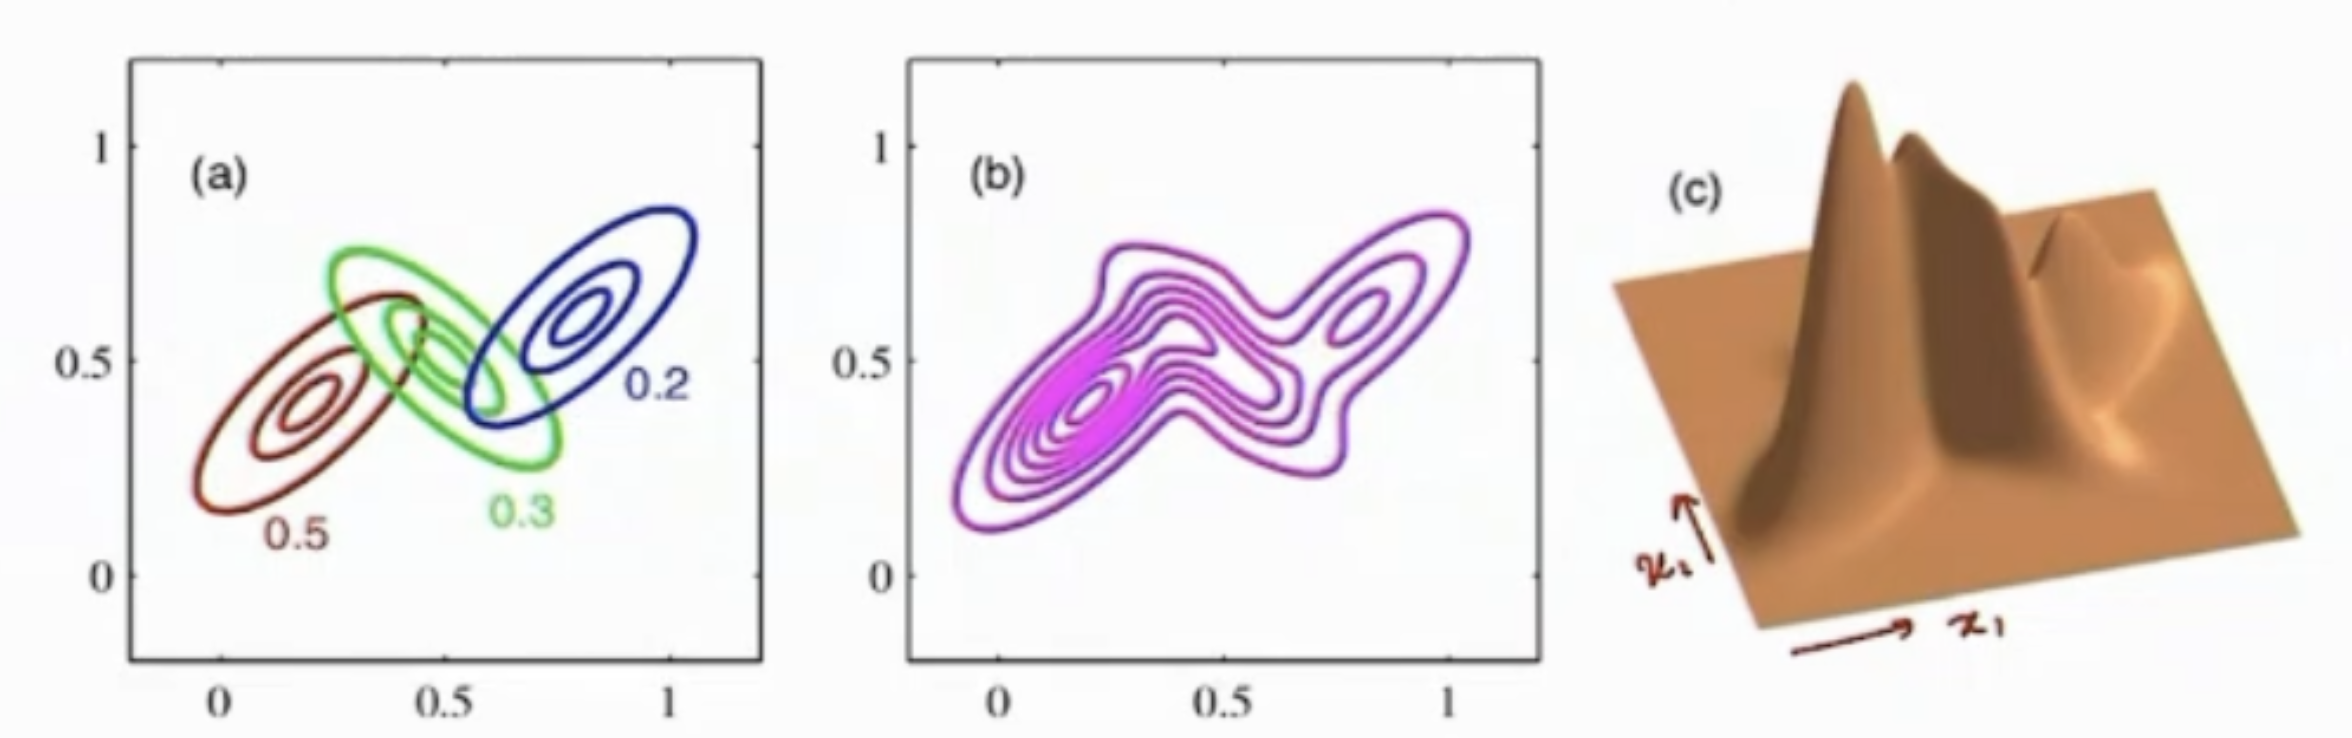
\includegraphics[width=0.75\linewidth]{images/gaussian_mixture_models_example_1.png}

\newpage

\subsection{GMM Notation}

Given $\bar x \in \R^d$

\[ 
	\begin{aligned}
		\gamma_1, \dots, \gamma_k &\quad \text{mixing weights}\\
		\mu_1, \dots, \mu_k &\quad \text{cluster means}\\
		\Sigma_1, \dots, \Sigma_k &\quad \text{cluster covariance matrices}\\
		\bar{\theta} = [\gamma_1, \dots, \gamma_k, \mu_1, \dots, \mu_k, \Sigma_1, \dots, \Sigma_k] &\quad \text{model parameters}\\
	\end{aligned}
\]

Assuming Gaussians are spherical, learned GMM:

\[ 
	\begin{aligned}
		z^{(i)} \sim \text{Categorical}(\bar{\gamma}) &\quad \text{cluster indicators}\\
		f(\bar x^{(i)} | z^{(i)}; \bar{\theta}) \sim \mathcal{N}(\bar{\mu}_{z^{(i)}}, \Sigma_{z^{(i)}}) &\quad \text{base distribution}\\
	\end{aligned}
\]

To calculate number of parameters for a GMM, we add mixing weights ($k-1$ parameters since mixing weights must sum to 1) + cluster means ($kd$ parameters) + cluster covariance matrices ($\frac {k(k-1)} 2 + k$ for general, $k$ for spherical)

\subsection{MLE of GMM with known labels}

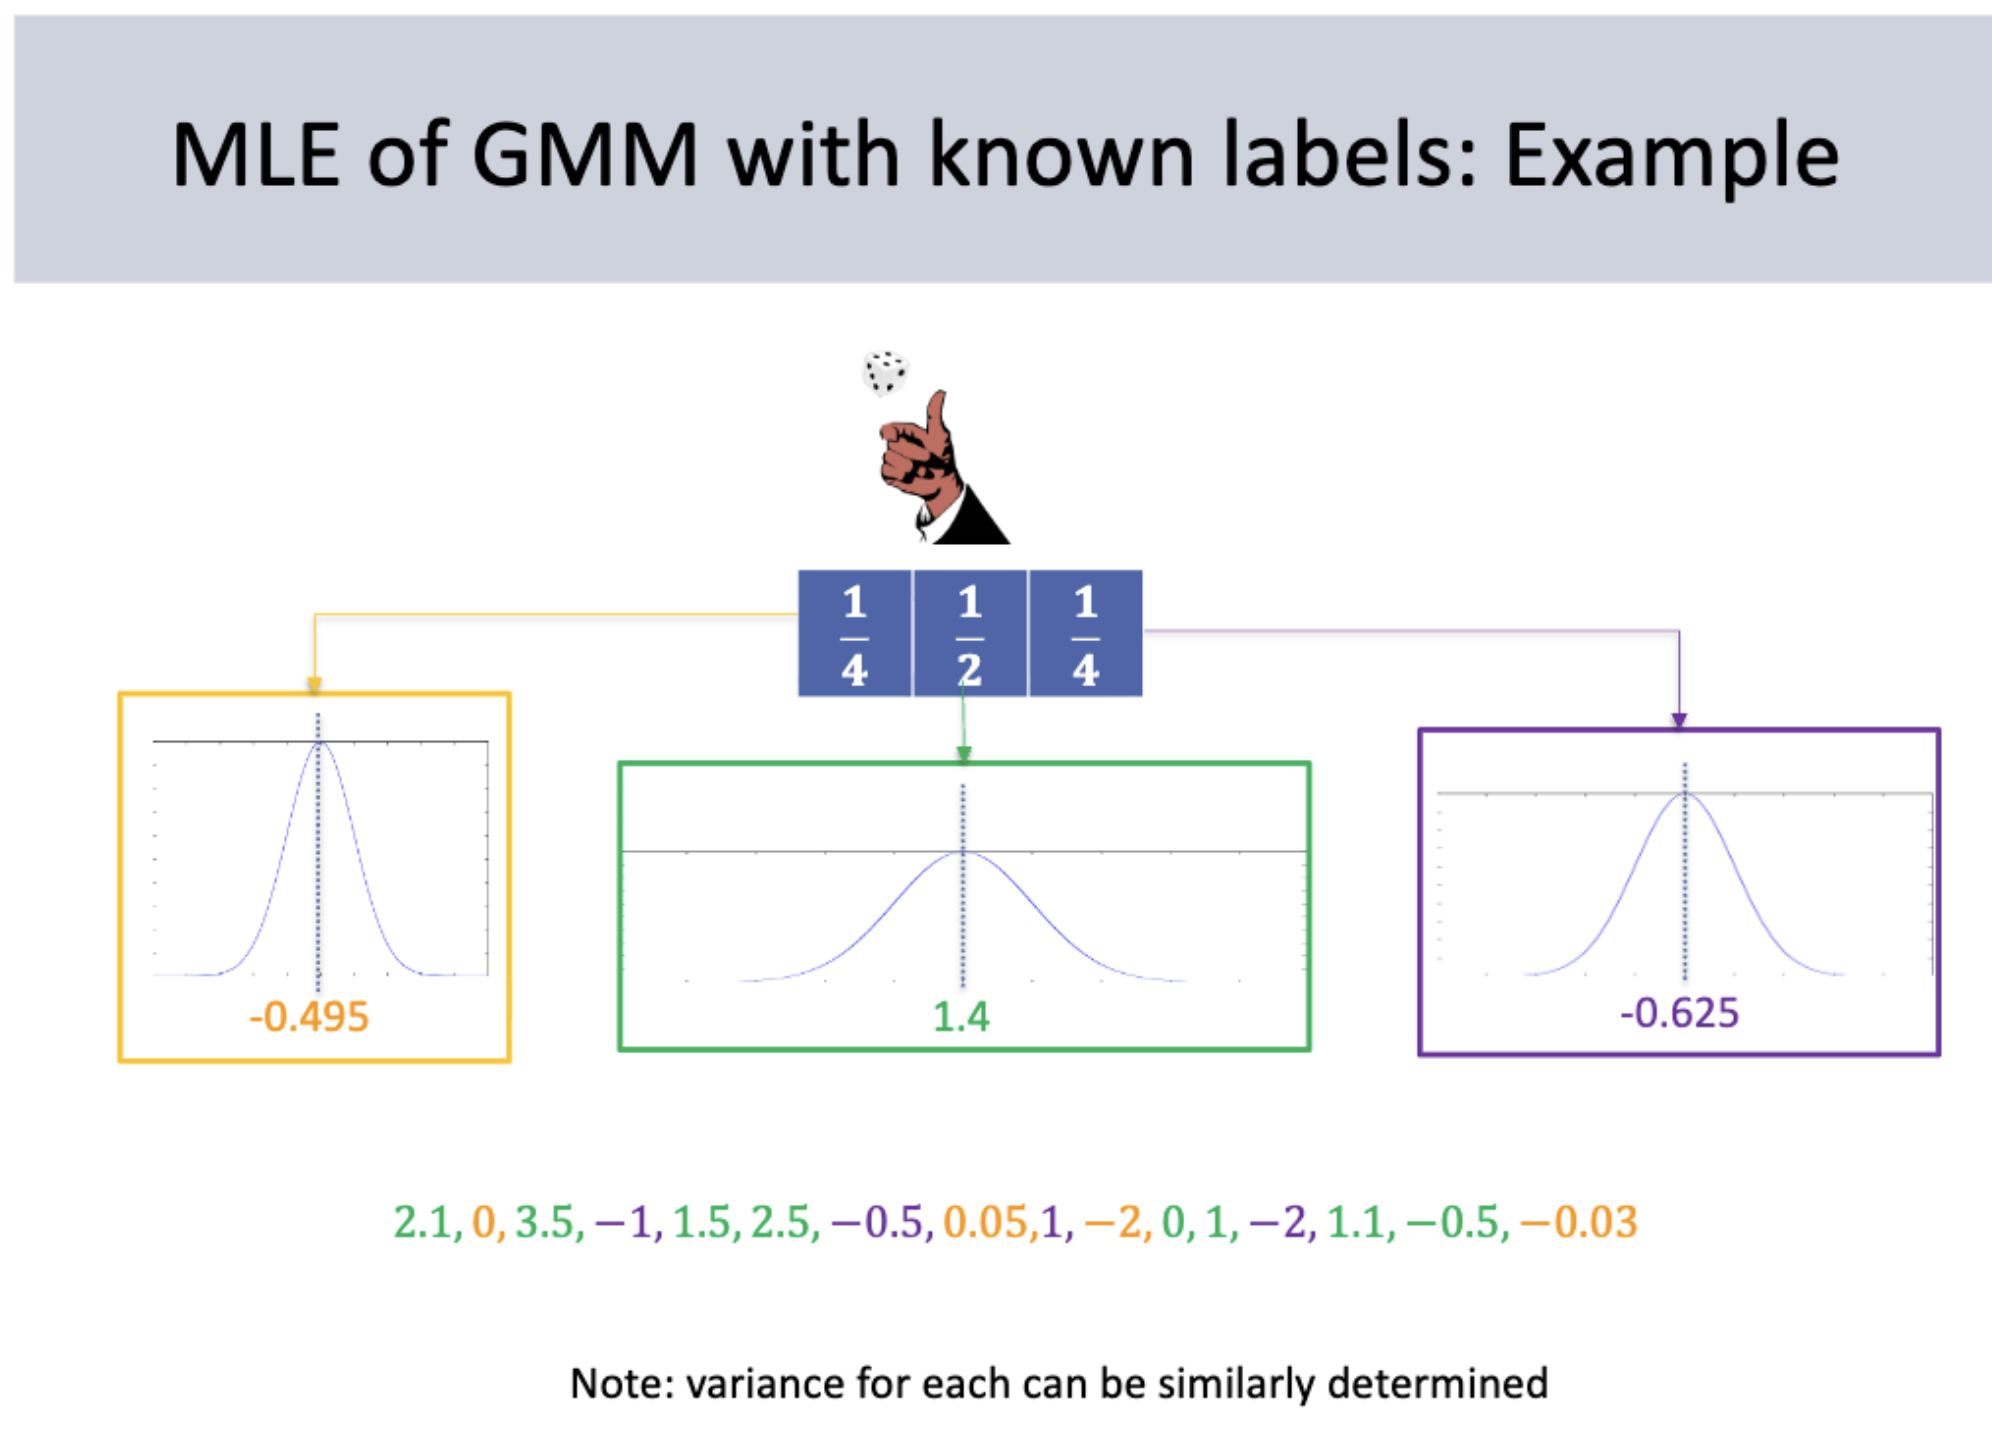
\includegraphics[width=0.75\linewidth]{images/gaussian_mixture_models_example_2.png}

In this example, we have a dataset with datapoints in $\R$ and each datapoint tells us which of 3 underlying gaussian distributions it is chosen from. Intuitively, we find the

\begin{itemize}
	\item mixing coefficients by counting the number of datapoints from each individual Gaussian distribution and dividing by the total number of datapoints
	\item Gaussian distribution parameters for distribution $i$ by using the MLE formulas above (section 32.5 in this case) on only the datapoints from Gaussian distribution $i$.
\end{itemize}

Analytically, we will define the MLE for this dataset and we expect the results to be what we intuitively want.

\subsection{Log-Likelihood for GMMs with known labels}
Let $\gamma_j$ be the chance of choosing the $j$-th distribution and indicator function

\[ 
	\delta(j|i) = \begin{cases}
		1 & \text{if $\bar{x}^{(i)}$ belongs to cluster $j$}\\
		0 & \text{otherwise}
	\end{cases}
\]

We define the probability $p(S_n)$ of getting dataset $S_n$ with $k$ distribution as follows:

\[ 
	\begin{aligned}
		p(S_n) &= \prod_{i=1}^n p(\bar{x}^{(i)}, y^{(i)})\\
					&= \prod_{i=1}^n p(\bar{x}^{(i)}|y^{(i)})p(y^{(i)})\\
					&= \prod_{i=1}^n \sum_{j=1}^k \delta(j|i) (\mathcal{N}(\bar x^{(i)}| \bar{\mu}^{(j)}, \sigma^2_j)\gamma_j)\\
	\end{aligned}
\]

and the log likelihood probability $l(S_n|\bar{\theta})$ with parameters of the GMM $\bar{\theta}$ as follows

\[ 
	\begin{aligned}
		l(S_n | \bar{\theta}) &= \ln \prod_{i=1}^n p(\bar{x}^{(i)}, y^{(i)} | \bar{\theta})\\
					&= \sum_{i=1}^n \ln p(\bar{x}^{(i)}, y^{(i)} | \bar{\theta})\\
					&= \sum_{i=1}^n \ln \left(\sum_{j=1}^k \delta(j|i) (\mathcal{N}(\bar x^{(i)}| \bar{\mu}^{(j)}, \sigma^2_j)\gamma_j)\right)\\
	\end{aligned}
\]

Here, we have a log of sums, which is generally hard to simplify. Luckily, since $\delta(j|i) = 1$ for exactly one $j$ for each $i$ and 0 otherwise, we can simplify to the following:

\[ 
	\begin{aligned}
		l(S_n | \bar{\theta}) &= \sum_{i=1}^n \ln \left(\sum_{j=1}^k \delta(j|i) (\mathcal{N}(\bar x^{(i)}| \bar{\mu}^{(j)}, \sigma^2_j)\gamma_j)\right)\\
													&= \sum_{i=1}^n \sum_{j=1}^k \delta(j|i) \ln (\mathcal{N}(\bar x^{(i)}| \bar{\mu}^{(j)}, \sigma^2_j)\gamma_j)\\
													&= \sum_{i=1}^n \sum_{j=1}^k \delta(j|i) \left(\ln \mathcal{N}(\bar x^{(i)}| \bar{\mu}^{(j)}, \sigma^2_j) + \ln \gamma_j\right)\\
	\end{aligned}
\]
\newpage
The MLE solutions are:

\begin{itemize}
	\item $\hat n_j = \sum_{i=1}^n \delta(j|i)$ (number of points assigned to cluster $j$)
	\item $\gamma_j = \frac {\hat n_j} n$ (number of points assigned to cluster $j$)
	\item $\bar{\mu}^{(j)} = \frac 1 {\hat n_j}\sum_{i=1}^n \delta(j|i) \bar x^{(i)}$ (mean of points in cluster $j$)
	\item $\sigma_j^2 = \frac 1 {d\hat n_j} \sum_{i=1}^n \delta(j|i) ||\bar x^{(i)} - \bar{\mu}^{(j)}||^2$ (mean squared distance of points in cluster $j$)
\end{itemize}

This is exactly the same as what we intuitively want.

\subsection{MLE for GMMs with unknown labels}

Finding the MLE parameters for a GMM with datapoints labeled is generally a very simple extension of finding MLE parameters for a single Gaussian distribution. The problem is that datapoints are almost never labeled. How do we find the parameters for a GMM from datapoints without labels?

\subsection{Expectation Maximization (EM) for GMMs: overview} \label{sub:33.4}

\textbf{Steps:}

\begin{enumerate}
	\item Initialize model parameters $\bar{\theta}$ and hyperparameters (e.g., $k$)
	\item Iterate until convergence:
		\begin{itemize}
			\item E step: use current estimate of mixture model to softly assign examples to a cluster
			\item M step: re-estimate each cluster model separately based on the points assigned to it (similar to the ``known label" case)
		\end{itemize}
\end{enumerate}

\subsection{Expectation Maximization for GMMs: E-Step}

fix $\bar{\theta} = [\gamma_1, \dots, \gamma_k, \bar{\mu}^{(1)}, \dots, \bar{\mu}^{(k)}, \sigma_1^2, \dots, \sigma_k^2] $. \\

Softly assign points to clusters according to posterior probability:

\[ p(j|i) = \frac {\gamma_j \mathcal{N}(\bar x^{(i)} | \bar{\mu}^{(j)}, \sigma_j^2)} {\sum_t \gamma_t \mathcal{N}(\bar x^{(i)} | \bar{\mu}^{(t)}, \sigma_t^2)} \]

Here is an illustration of what this step would look like:

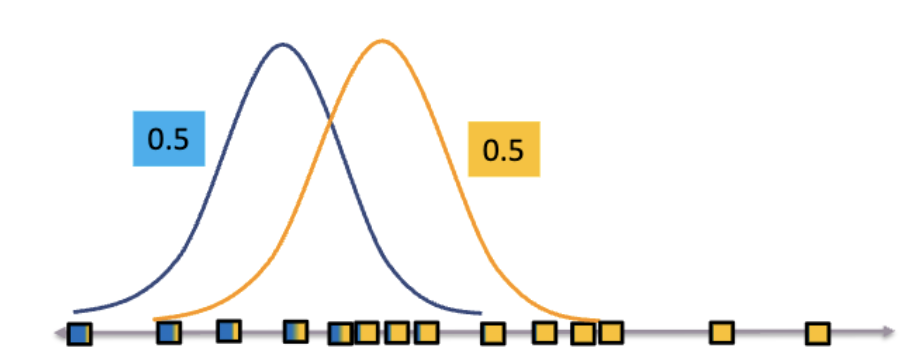
\includegraphics[width=0.75\linewidth]{images/em_algorithm_example_1.png}

\newpage

\subsection{Expectation Maximization for GMMs: M-Step}

Optimize each cluster separately given $p(j|i)$. These formulas will look very similar to before, only in the place of discrete labels $\delta(j|i)$, we will use the soft clustering proportions $p(j|i)$ we found in the E-Step:

\begin{itemize}
	\item $\hat n_j = \sum_{i = 1}^n p(j|i)$. 
	\item $\hat{\bar{\mu}}^{(j)} = \frac 1 {\hat n_j} \sum_{i = 1}^n p(j|i) \bar x^{(i)}$
	\item $\hat{\gamma}_j = \frac {\hat n_j} n$
	\item $\hat{\sigma}_j^2 = \frac 1 {d \hat n_j} \sum_{i=1}^n p(j|i)||\bar x^{(i)} - \hat{\bar{\mu}}^{(j)}||^2$ \quad ($d$ is the dimensionality of the gaussian/input)
\end{itemize}


\textbf{Note:} How is this possible? We can't use the same trick as before to get rid of the log of a summation since we don't have the fact that $p(j|1) = 1$ for exactly one $j$ for each $i$ and 0 otherwise, hence we don't have the equality:

\[ \ln \left( \sum_{j=1}^k p(j|i)\left( \mathcal{N}(\bar x^{(i)} | \bar{\mu}, \sigma_j^2 \right)\gamma_j \right) = \sum_{j=1}^k p(j|i) \ln \left( \mathcal{N}(\bar x^{(i)} | \bar{\mu}, \sigma_j^2) \gamma_j \right) \]

This is the response from piazza: Long story short, you can use Jensen's inequality to show that the right term represents a lower bound of the left term. So by optimizing the parameters using the lower bound in the M step we can improve the log likelihood of the data.

\subsection{Properties of the EM algorithm}

\begin{itemize}
	\item each iteration improves log-likelihood
		\begin{itemize}
			\item E step never decreases log-likelihood
			\item M step never decreases log-likelihood
		\end{itemize}
	\item EM converges to a (local) optimum
\end{itemize}

\subsection{Model Selection: How to pick $k$}

To pick $k$ (number of distributions in our mixture of distributions), one naive first idea is to find $k$ with the highest log-likelihood of creating the dataset. However, similar to $k$-means, a higher value of $k$ will essentially always lead to a higher log-likelihood until you have $k = n$, at which point the optimal mixture of distributions will be a distribution per datapoint, which is absolutely nonsensical.\\

A better way to pick $k$ is similar to the idea of regularization that we've seen in the past. Instead of purely optimizing for the log-likelihood, we will optimize for the following Bayesian Information Criterion (BIC) formula:

\[ BIC(S_n;\bar{\theta}) = l(S_n;\bar{\theta}) - \frac {\#param} 2 \log(n) \]

As you can see in the following picture, optimizing for BIC gives us a more satisfying number of clusters ($k = 3$) rather than optimizing for $l$ directly.

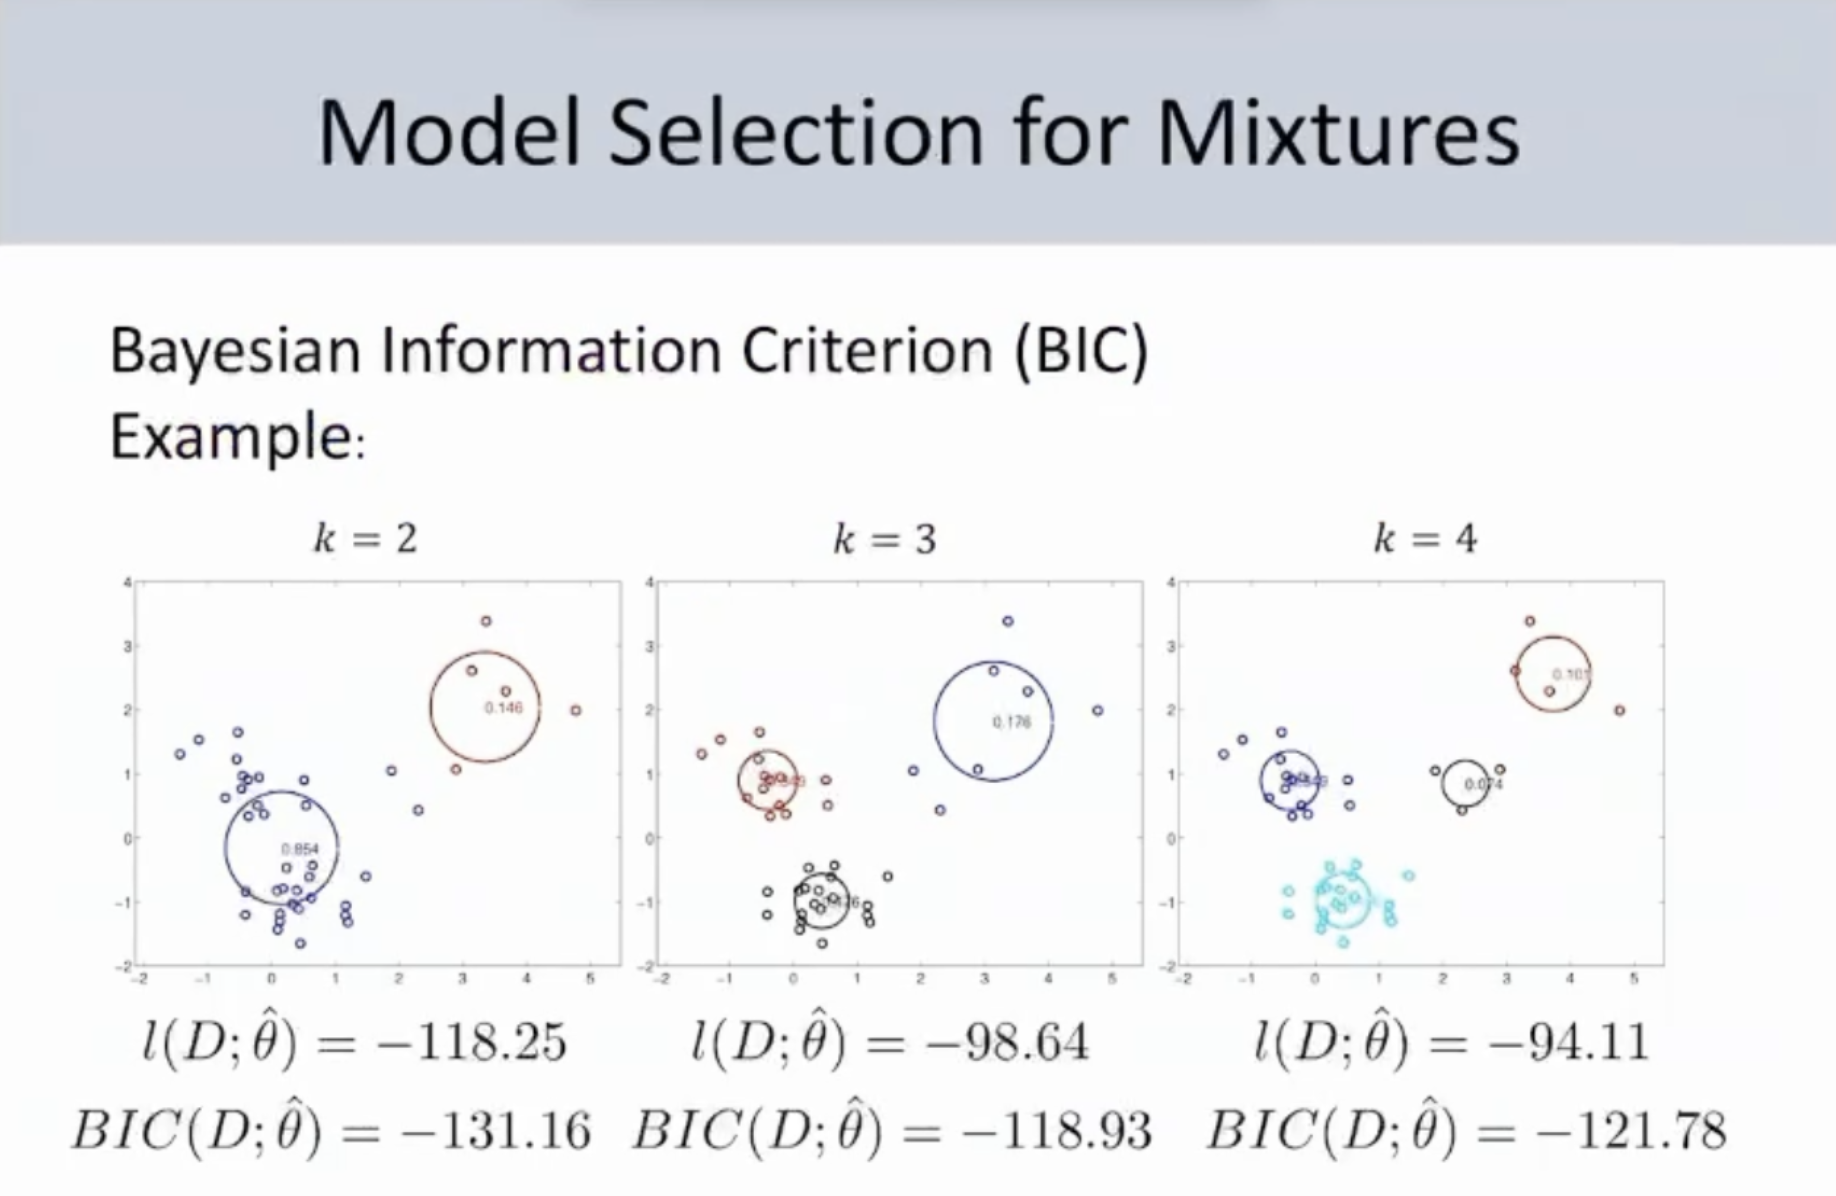
\includegraphics[width=0.75\linewidth]{images/em_algorithm_example_2.png}

\section{Bayesian Networks}

A Bayesian network is a probabilistic graphical model that represents a set of variables and their conditional dependencies via a directed acyclic graph (DAG). The purpose of a Bayesian Network is to represent, reason about, and predict complex systems involving uncertainty, specifically by mapping variables and their conditional dependencies.\\

\textbf{Note:} For our discussions of Bayesian Networks, we will keep our scope to only discrete random variables.

\subsection{Why use Bayesian Networks}

\begin{itemize}
	\item Savings in number of parameters
	\item Also captures dependencies which makes it easier to learn and infer
	\item For inference
		\begin{itemize}
			\item Can compute marginal probabilities
				\begin{itemize}
					\item $Pr(x_3)$
				\end{itemize}
			\item Can compute conditional probabilities
				\begin{itemize}
					\item $Pr(x_3 | x_1)$
				\end{itemize}
		\end{itemize}
\end{itemize}

\subsection{Probability refresher}

Suppose you are given random variables

\begin{itemize}
	\item Sunshine $S \in \{ 0, 1 \}$
	\item Rain $R \in \{ 0, 1 \}$
\end{itemize}

Then

\begin{itemize}
	\item their join distribution $Pr(S,R)$ is\\
		\begin{tabular}{|c|c|c|}
			\hline
			$s$ & $r$ & $Pr(S=s, R=r)$ \\
			\hline
			0 & 0 & 0.2\\
			\hline
			0 & 1 & 0.08\\
			\hline
			1 & 0 & 0.7\\
			\hline
			1 & 1 & 0.02\\
			\hline
		\end{tabular}~\\
	\item the marginal distribution $Pr(S)$ is\\
		\begin{tabular}{|c|c|}
			\hline
			$s$ & $Pr(S=s)$ \\
			\hline
			0 & 0.28\\
			1 & 0.72\\
			\hline
		\end{tabular}~\\
	\item and the conditional distribution $Pr(S|R)$ is\\
		\begin{tabular}{|c|c|}
			\hline
			$s$ & $Pr(S=s | R=1)$ \\
			\hline
			0 & 0.8\\
			1 & 0.2\\
			\hline
		\end{tabular}~\\
\end{itemize}

\subsection{Two notions of Independence}

\textbf{Marginal Independence:}

\[ Pr(X_1, X_2) = Pr(X_1)Pr(X_2) \]
\[ X_1 \perp X_2 \]
\[ Pr(X_1 | X_2) = Pr(X_1) \]

\textbf{Conditional Independence:}

\[ Pr(X_1, X_2 | X_3) = Pr(X_1|X_3)Pr(X_2|X_3) \]
\[ X_1 \perp X_2 | X_3 \]
\[ Pr(X_1 | X_2,X_3) = Pr(X_1|X_3) \]

\subsection{Bayesian Networks: factorization}

\begin{itemize}
	\item Recall chain rule of probability
		\[ p(X_1, \dots, X_d) = p(X_1| X_2, \dots, X_d)p(X_2| X_3, \dots, X_d) \dots p(X_{d-1}| X_d)p(X_d) \]
	\item Bayesian Networks encode marginal and conditional independencies (see section \ref{sub:34.8}).
	\item Thus, for a given graph, the joint distribution can be written as a product of the conditional probability of each variable given its parents.
		\begin{itemize}
			\item Variables $X_1, \dots, X_d$
			\item Parents of variable $X_i$ represented by $X_{pa_i}$
				\[ P(X_1, \dots, X_d) = \prod_{i=1}^d P(X_i | X_{pa_i}) \]
		\end{itemize}
\end{itemize}

\subsection{Bayesian Networks by Example}

Let $x_1$ and $x_2$ be random variables for the event of two independent, fair coin flips. Let $x_3$ be a third random variable that takes on the value 1 when $x_1 == x_2$ and 0 otherwise. In otherwords, 

\[ Pr(x_3 = 1 | x_1 == x_2) = 1 \quad \text{and} \quad Pr(x_3 = 0 | x_1 \ne x_2) = 1\]

Then we can create the following Bayesian graph:

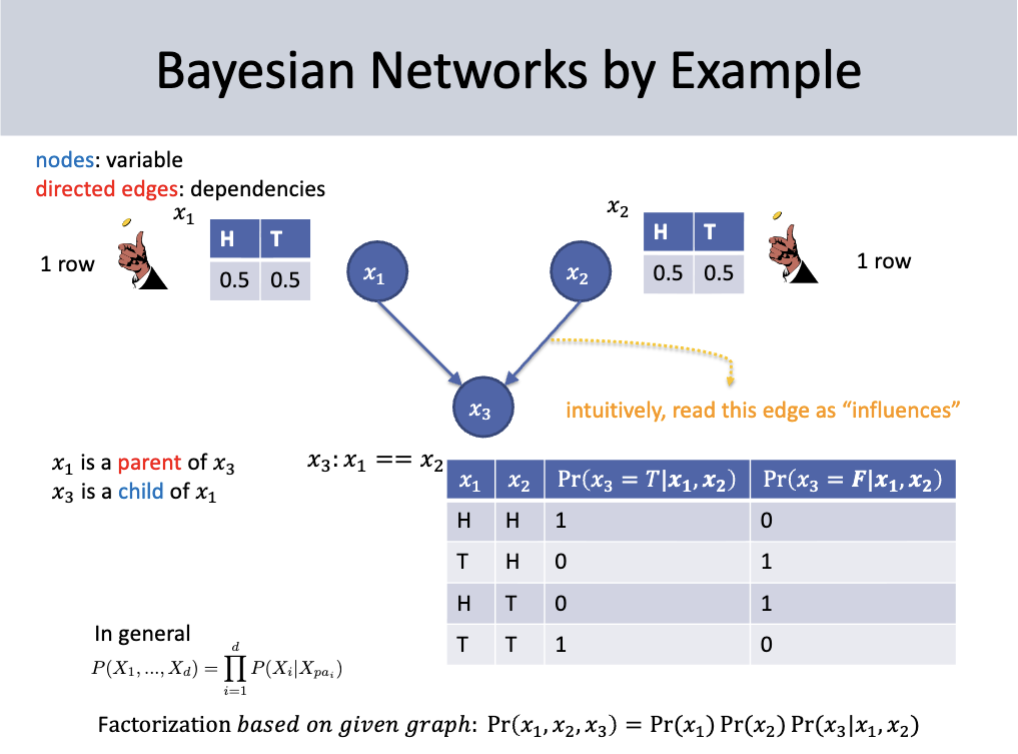
\includegraphics[width=0.75\linewidth]{images/bayesian_networks_example_1.png}

As shown from the picture and section 34.4, you can calculate the probability of an outcome of this specific Bayesian Network by using the formula

\[ P(x_1, x_2, x_3) = Pr(x_1) Pr(x_2) Pr(x_3 | x_1, x_2) \]

\subsection{Marginal Independence: Example}

Claim: $x_1$ and $x_2$ from the previous example are marginally independent of each other. That is, we want to show that $Pr(x_1, x_2) = Pr(x_1)Pr(x_2)$:

\[ Pr(x_1,x_2,x_3) = Pr(x_1)Pr(x_2)Pr(x_3|x_1, x_2) \]

\[ 
	\begin{aligned}
		Pr(x_1, x_2) &= \sum_{x_3} Pr(x_1, x_2, x_3)\\
								 &= \sum_{x_3} Pr(x_1)Pr(x_2)Pr(x_3|x_1, x_2)\\
								 &= Pr(x_1)Pr(x_2) \sum_{x_3} Pr(x_3|x_1, x_2)\\
								 &= Pr(x_1)Pr(x_2)
	\end{aligned}
\]

So $x_1 \perp x_2$

\subsection{Conditional Independence: Example}

However, $x_1$ and $x_2$ are conditionally dependent given $x_3$. To see this, note that if we only knew the value of $x_3$, we wouldn't immediately know the value of $x_1$. However, if we knew both $x_3$ and $x_2$, we would instantly know the value of $x_1$. Thus,

$Pr(X_1 | X_2, X_3) \ne Pr(X_1 | X_3)$.

Sp $X_1$ is not conditionally independent from $X_2$. This shows that marginal independence does not imply conditional independence, and vice versa.

\subsection{Inferring Independence (d-separation)} \label{sub:34.8}

\textbf{Steps}:\\
1. keep only ancestral graph of all observed variables\\
2a. connect nodes with common (immediate) child. This is different from connecting nodes with common descendants.\\
2b. make graph undirected\\
3. read off property:
\begin{itemize}
	\item If there is no path between variables of interest, then they are marginally independent
	\item If all paths between variables of interest go through a particular node $x_0$, then the variables are independent given $x_0$.
		\begin{itemize}
			\item Intuitively, we can say that node $x_0$ ``blocks" the influence from the first variable to the second
			\item \textbf{Note:} for $X_1 \perp X_2 | \{ X_3, X_4 \}$, each path has to go through at least one of the nodes in the set $\{ X_3, X_4 \}$.
		\end{itemize}
\end{itemize}

\subsection{Inference: Example}

Lets say we have the following Bayesian Network:

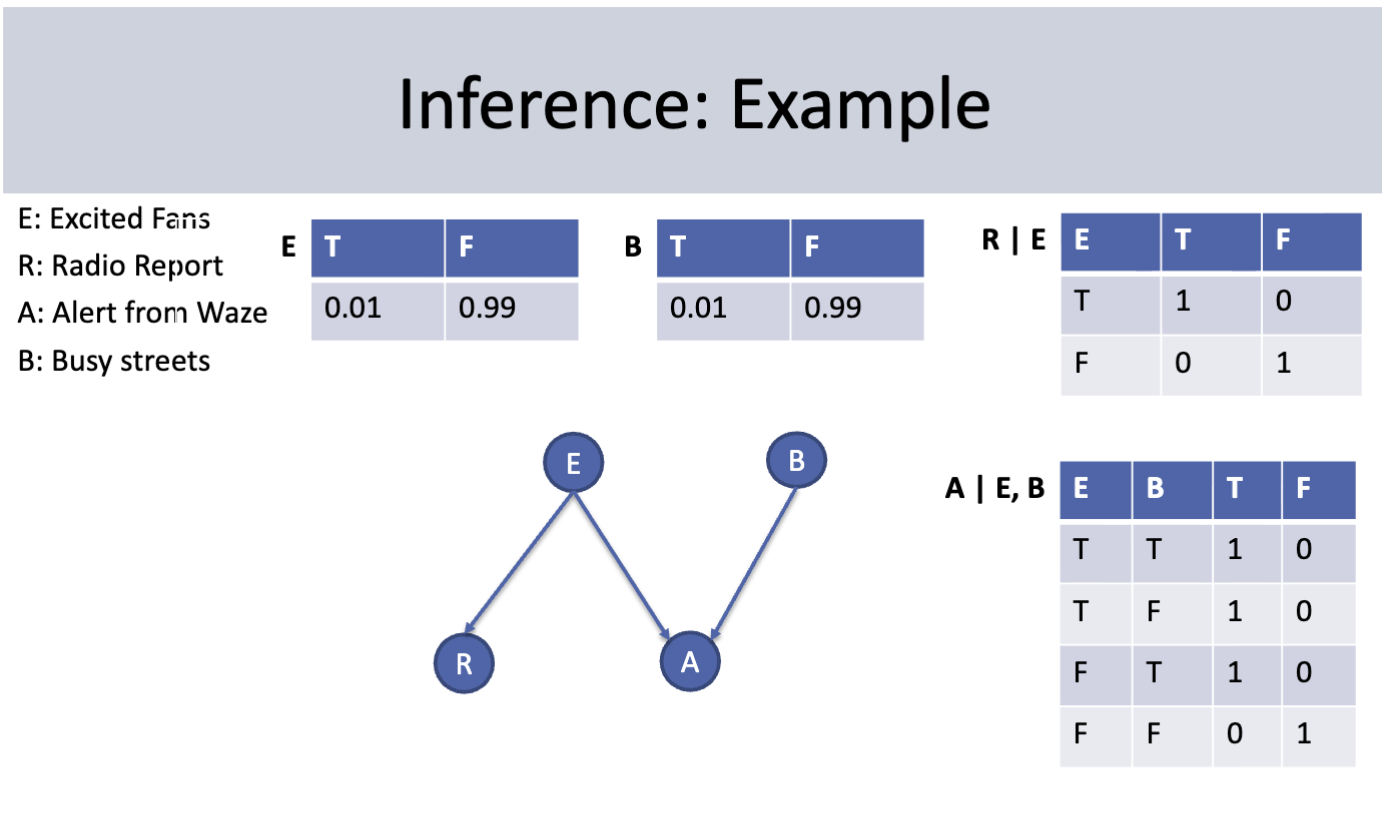
\includegraphics[width=0.75\linewidth]{images/bayesian_networks_example_2.png}

Suppose we observe $A = T$. Intuitively, we would expect the probability $P(B = T)$ to increase (specifically, to near 50\% because of how $A$ is defined, and $E$ and $B$ having the same distributions). To actually compute we calculate, we use the definition of conditional probability:

\[ 
	\begin{aligned}
		P(B=T|A=T) &= \frac {P(B=T, A=T)}{P(A=T)} & \text{(def. of conditional probability)}\\
							 &= \frac {P(B=T, A=T)}{\sum_b P(B=b, A=T)} & \text{(sum rule)}
	\end{aligned}
\]

Note that

\[ 
	\begin{aligned}
		P(B=b,A=a) &= \sum_e \sum_r P(B=b,A=a,E=e,R=r)\\
							 &= \sum_e \sum_r P(E=e) P(B=b) P(R=r|E=e) P(A=a|E=e, B=b)\\
							 &= P(B=b) \sum_e P(E=e) P(A=a|E=e, B=b) \sum_r P(R=r|E=e)\\
							 &= P(B=b) \sum_e P(E=e) P(A=a|E=e, B=b)\\
	\end{aligned}
\]

We get the last equality since $\sum_r P(R=r|E=e) = 1$. So we get

\[ P(B=T|A=T) = \frac {P(B=b) \sum_e P(E=e) P(A=a|E=e, B=b)} {\sum_b P(B=b) \sum_e P(E=e) P(A=a|E=e, B=b)}\]

After plugging in values, we get

\[ P(B=T|A=T) = \frac 1 {1.99} \approx \frac 1 2 \]

\section{Learning Bayesian Networks}

Two main problems:

\begin{enumerate}
	\item estimate parameters (conditional probabilities) given graph structure and data
		\begin{itemize}
			\item Easier problem to solve
		\end{itemize}
	\item Search over possible graph structures (i.e., graph nodes and edges)
		\begin{itemize}
			\item Harder problem to solve
		\end{itemize}
\end{enumerate}

\subsection{Learning parameters in a Bayesian Network}

Given a Bayesian graph and a dataset, we simply count the proportions in our dataset to get the conditional probabilities:

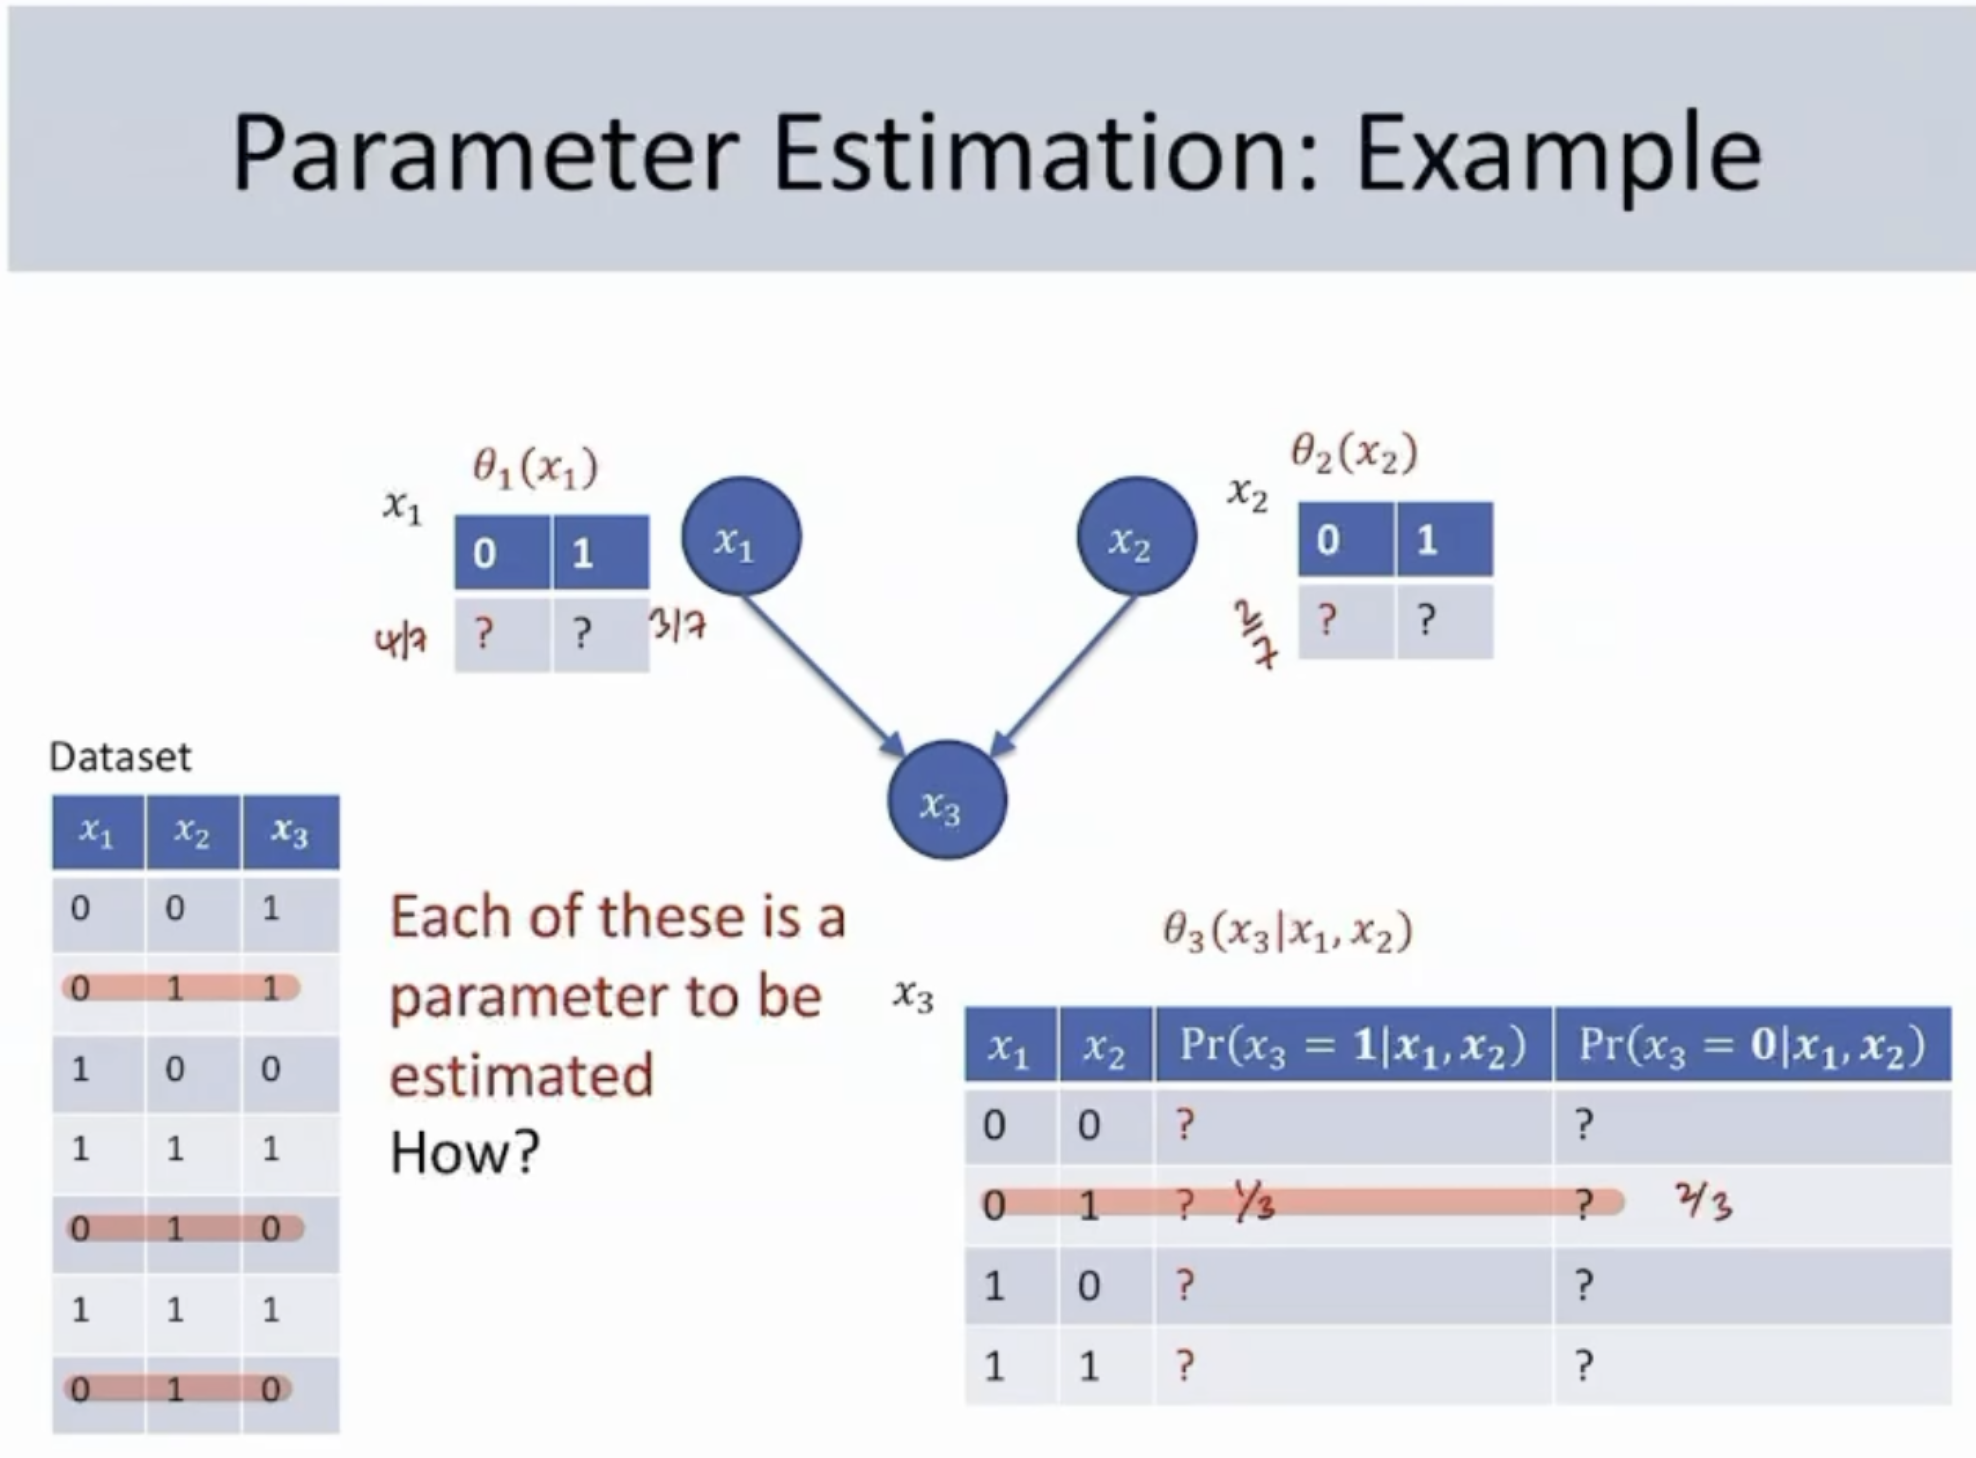
\includegraphics[width=0.75\linewidth]{images/learning_bayesian_networks_example_1.png}

Intuitively, this makes sense to do, but we can prove that this is optimal through MLE.

\newpage

\subsection{Bayesian Networks Parameter Estimation (MLE)}

Suppose we have $d$ discrete random variables $x_1, \dots, x_d$ and each $x_i \in V_i$ where $V_i = \{ v_1, v_2, \dots, v_{k_i}\}$ ($k_i$ is a variable the number of possible values that $i$th random variable can take on). Additionally, suppose we have $n$ complete overservations

\[ S_n \left\{ \left[ x_1^{(t)}, \dots, x_d^{(t)} \right] \right\}_{t=1}^n \]

The log-likelihood of a conditional probability function $\theta$ given the dataset is

\[ l(\bar{\theta};S_n, G) = \ln \prod_{t=1}^n \prod_{i=1}^d \theta_i(x_i^{(t)} | x_{pa_i}^{(t)}) = \sum_{t=1}^n \sum_{i=1}^d \ln \theta_i (x_i^{(t)}| x_{pa_i}^{(t)}) \]

where the first product is the result of the datapoints being i.i.d. and the second product is a result from the factorization rules of Bayesian networks. The corresponding MLE becomes

\[ \hat{\theta}_i (x_i = v_i | x_{pa_i} = v_{pa_i}) = \frac {n(x_i = v_i, x_{pa_i} = v_{pa_i})} {\sum_{v_i'} n(x_i = v_i', x_{pa_i} = v_{pa_i})} \]

where $n(x_i, x_{pa_i})$ is the number of observations in $S_n$ where $X_i = x_i$ and $X_{pa_i} = x_{pa_i}$

\subsection{Learning Graph Structure}

\textbf{First idea}: Choose graph structure that maximizes log likelihood\\
\textbf{Issue}: A graph with a superset of edges always results in a higher log-likelihood since there are more parameters in child nodes to play with, which means we can more easily overfit to the dataset.\\
\textbf{Fix}: Instead of optimizing solely on log-likelihood of parameters, we optimize for BIC (same idea as regularization):

\[ BIC(S_n;\bar{\theta}) = l(S_n;\bar{\theta}) - \frac k 2 \log(n). \]

with $k$ being the total number of parameters. To solve for $k$, suppose each random variable $x_i$ can take on $r_i$ possible values for $i = 1, \dots, m$:

\[ k = \sum_{i=1}^m (r_i - 1) \prod_{j \in pa_i} r_j \]

\section{Reinforcement Learning}

\subsection{Reinforcement Learning: Success Stories}

\begin{itemize}
	\item AlphaGo
		\begin{itemize}
			\item Modeled Go as a supervised learning problem using human expert moves
			\item Used neural networks and Reinforcement learning
		\end{itemize}

	\item AlphaGo Zero
		\begin{itemize}
			\item model was only provided game rules
			\item no other human data, guidance, or domain knowledge was given
			\item All the model could do was play against itself millions, maybe even billions of times
		\end{itemize}

	\item MuZero
		\begin{itemize}
			\item model was given the rules of an arbitrary game
			\item Same as AlphaGo Zero, the model wasn't given any other assistance. All it could do was play itself
			\item The model eventually would be able to play any game extremely well
		\end{itemize}

\end{itemize}

Specifically, with AlphaGo Zero, in 3 days it was able to beat the model of AlphaGo that beat Lee Sedol, and in 40 days, it outperformed every other model made for Go, effectively becoming the best Go player in the world.\\

Another examples of Reinforcement learning use cases is a robot teaching itself to walk rather than having it learn through direct programming or mimicry.\\

OpenAI popularized the notion of Reinforcement Learning with Human Feedback (RLHF), which utilizes a reward model that a human creates to create a superior model.

\subsection{Reinforcement Learning: Overview}

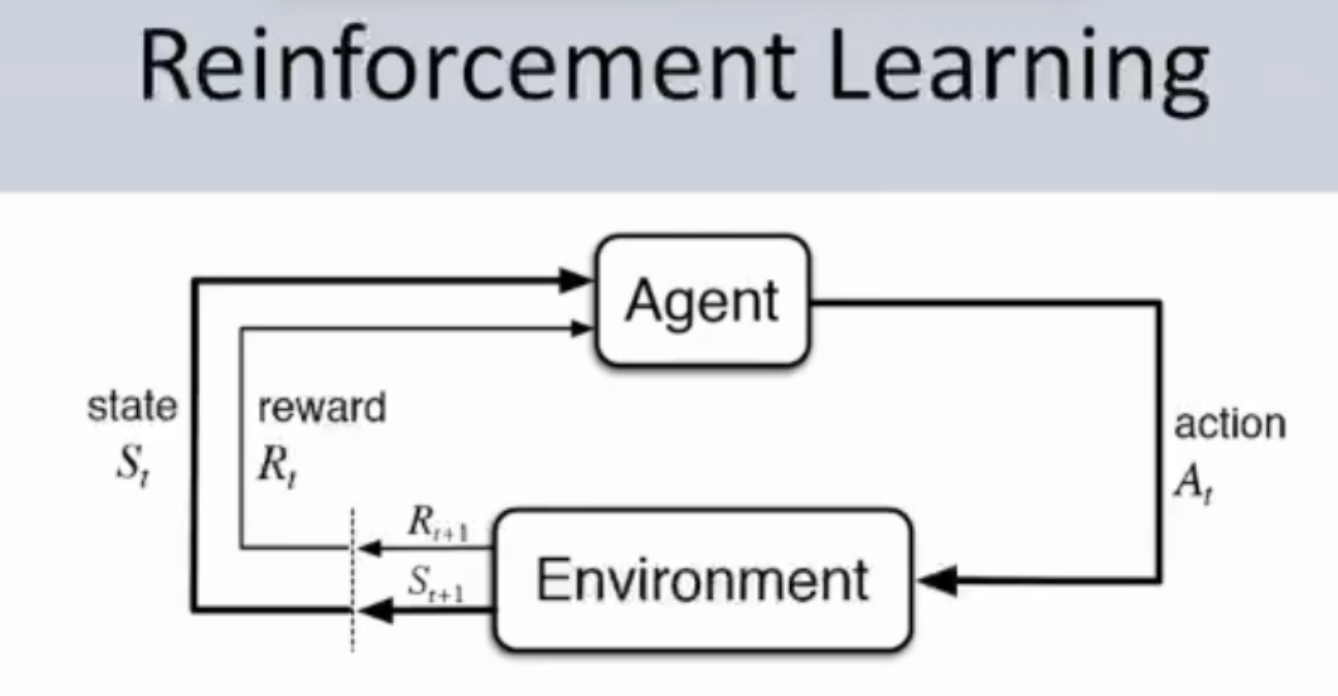
\includegraphics[width=0.75\linewidth]{images/reinforcement_learning_example_1.png}

In Reinforcement learning, there are two main puzzle pieces: The Agent and the Environment. The agent is some entity that iteratively observes the state it sees from the environment and does actions to explore new states and rewards from the environment. The environment has a state that gets changed by the agent's actions. Our goal is to train the agent so that it does actions that ultimately lead it to good circumstances (high reward) or states in the environment. Additionally, it is often perferrable to think of a reninforcement learning problem as a game, since it is usually very clear when a strategy is beneficial and when a strategy isn't through the result (win/loss) of a game.\\

This is different from supervised learning:
\begin{itemize}
	\item learner does not receive a passively labeled dataset
		\begin{itemize}
			\item actively collects information by interacting with the environment
		\end{itemize}
	\item environment is not fixed
		\begin{itemize}
			\item may vary as a result of actions
		\end{itemize}
	\item no fixed distribution from which all instances are drawn
\end{itemize}

\subsection{Markov Decision Processes}

We can model a reinforcement learning problem as a Markov Decision process (MDP) with

\[ s_t \in \mathcal{S}, \quad a_t \in \mathcal{A}, \quad r_t \in \mathcal{R} \subset \R \]

where $s_t$ is the state, $a_t$ is the action, and $r_t$ is the reward at time $t$. In a finite MDP, the sets $\mathcal{S}$, $\mathcal{A}$, and $\mathcal{R}$ are all finite sets, and the random variable $r_t$ and $s_t$ have well defined discrete probability distributions dependent only on the preceding state and action. The transition probabilites (also known as dynamics) of the MDP is defined by

\[ p(s_{t+1}, r_{t+1} | s_t, a_t). \]

\newpage

\subsection{Value and Policy functions}
\begin{itemize}
	\item $\pi(a|s)$ is called the policy function and specifies a distribution of the Action space $\mathcal{A}$ given a state $\mathcal{S}$. If a policy function always chooses a specific action for each state (i.e., each state has a probability of 1 for a specific action), it is considered a deterministic policy and is denoted at $\pi(s)$.\\

		\textbf{Note:} every finite MDP has an optimal deterministic policy (wrt total discounted reward). This can be seen from the Bellman Equation (subsection \ref{sub:36.7}) and the fact that a finite number of deterministic policies means that one or more must yield the highest possible reward. An optimal deterministic policy may fail to exist in other environment like Partially Observable Markov Decision Policies (POMDPs).
	\item discounted return $g_t$
		\[ g_t = r_{t+1} + \gamma r_{t+2} + \gamma^2 r_{t+3} + \cdots = \sum_{k=0}^{\infty} \gamma^k r_{t+k+1} = r_{t+1} + \gamma g_{t+1}  \]

		where $0 < \gamma < 1$ is a discount rate. This is similar to the idea of reverse interest. If you need to calculate $g_t$ for multiple values of $t$, then start with later time steps and calculate earlier values recursively using the recursive definition.

	\item Value funciton $v_{\pi}(s) = E_{\pi}[g_t|s_t = s]$. In other words, this is a function that measures the value of a state $s$ under some policy function $\pi$ by evaluating the discounted return in this state $s$.

	\item Optimal policy:
		\begin{itemize}
			\item $\pi \ge \pi'$ iff $\forall s \in \mathcal{S}, v_{\pi} \ge v_{\pi'} (s)$
			\item The policy that is at least as good as all other policies is an optimal policy
		\end{itemize}
\end{itemize}

\subsection{Reward Hypothesis}

What we mean by goals can be thought of as the maximization of the expected value of the cumulative sum of the received reward (a scalar quantity). The use of a reward signal to formalize the idea of a goal is one of the most distinctive features of reinforcement learning.

\subsection{Reinforcement Learning: Example}

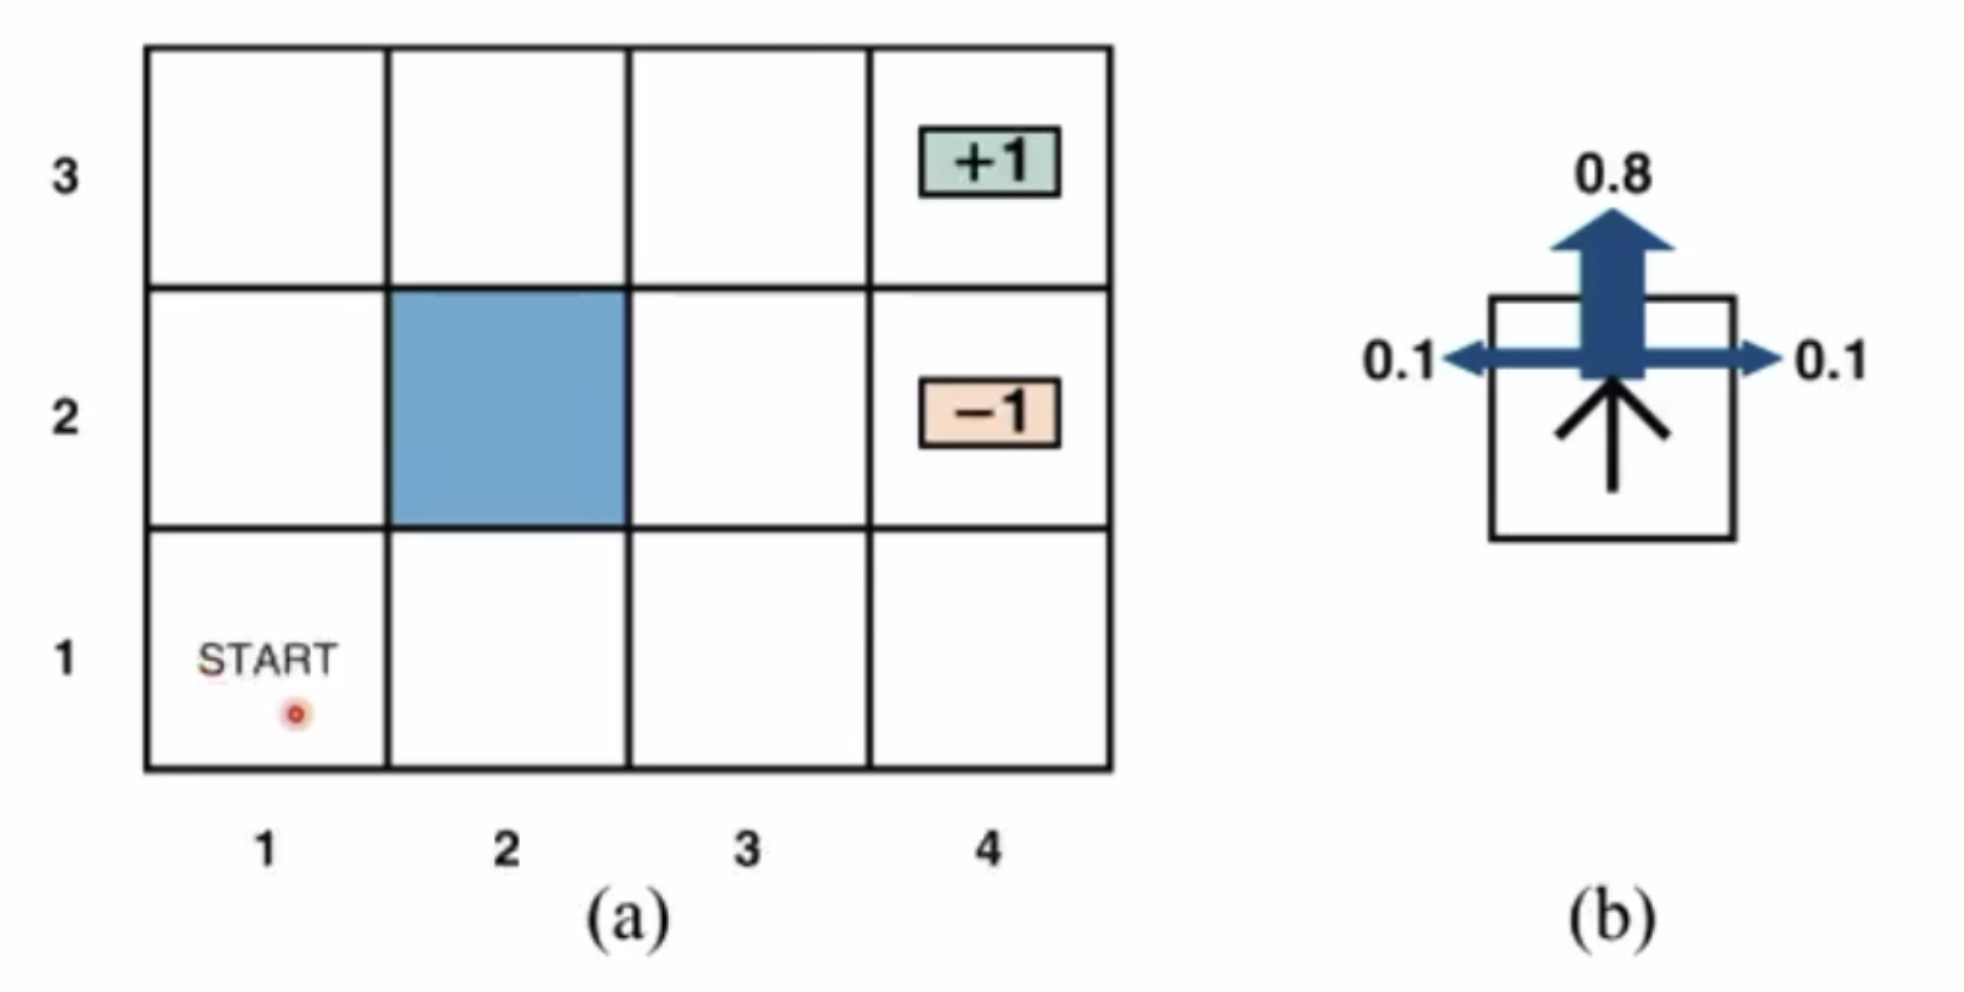
\includegraphics[width=0.75\linewidth]{images/reinforcement_learning_example_2.png}

In the example above, we have our a robot (our agent) start in the cell labeled start (1,1). The environment is a 4x3 grid. The actions in each cell are given by $a \in \{ Up, Down, Left, Right \}$, except for the cell labeled +1 (4,3) and -1 (4,2), which are terminal cells and which end the game if the agent ever gets to. If the robot chooses a specific direction to go, it has the probability distribution show on the right of the figure, i.e., if it chooses to go in a direction $a$, it has an 80\% chance of going in that direction and a 10\% chance of going in either orthogonal directions. A collision with a wall results in no movement. All transitions (other than transitions into terminal cells) have a reward of $r = -0.04$. With this, we get the following optimal policy:

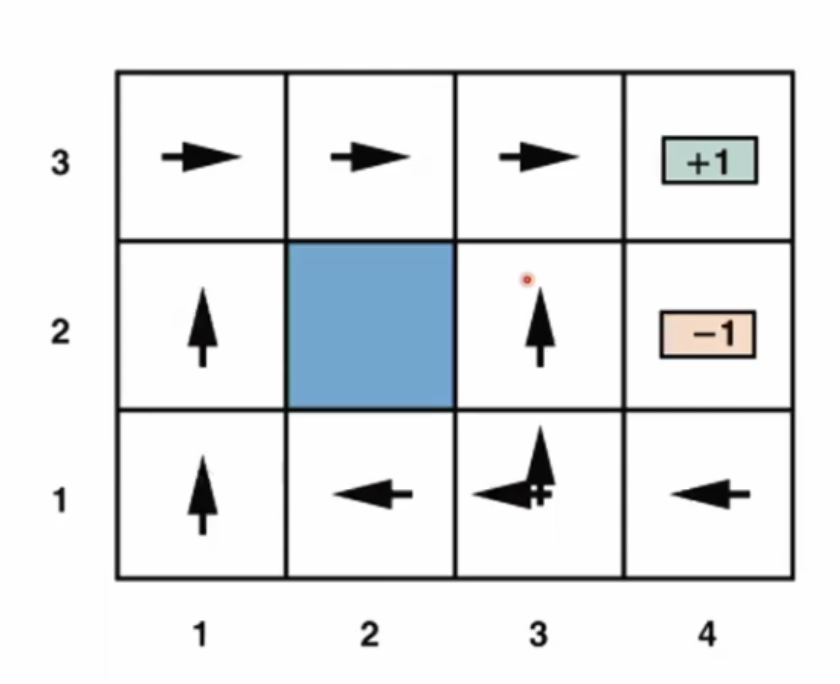
\includegraphics[width=0.75\linewidth]{images/reinforcement_learning_example_3.png}

where a single arrow in a state represents a deterministic policy and multiple arrows represents a non-deterministic policy. The policy at state (3,1) is particularly interesting. This optimal policy is telling us that it's optimal to choose both left and up in that particular state. This is due to how the math works out with $r=-0.04$ for every transition, and because in state (3,2), you have a much more likely chance of moving to the -1 state compared to the long way around.\\

Obviously, the optimal policy changes as your reward for each transition changes. Here are the optimal policies given different values of $r$:

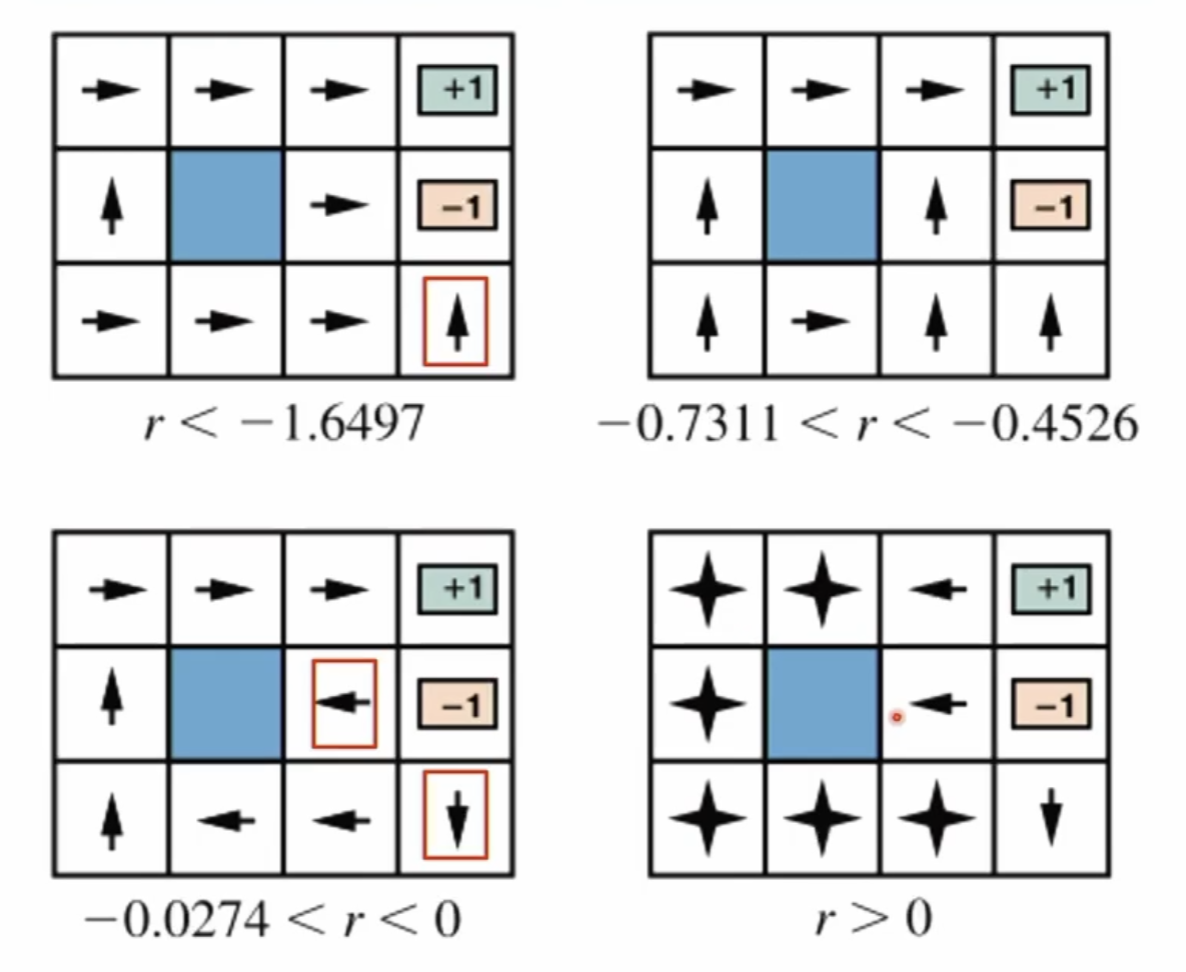
\includegraphics[width=0.75\linewidth]{images/reinforcement_learning_example_4.png}

\subsection{Bellman Equation} \label{sub:36.7}

The solution for an agent that tries to find a policy that maximizes expected total discounted reward is given by the Bellman Equation:

\[ 
	\begin{aligned}
		V^{\pi}(s) &= E\left[ \sum_{t=0}^{\infty} \gamma^t R(s_t, a_t) \big| s_0 = s, a_t \sim \pi(\cdot | s_t), s_{t+1} \sim P(\cdot | s_t, a_t)  \right]\\
							 &= E_{a \sim \pi(\cdot | s)} [R(s,a) + \gamma E_{s' \sim P(\cdot | s,a)} [V^{\pi} (s')]]\\
							 &= \sum_{a \in \mathcal{A}} \pi(a|s) \left( R(s,a) + \gamma \sum_{s' \in \mathcal{S}} P(s'|s,a) V^{\pi}(s') \right)
	\end{aligned}
\]

For deterministic $\pi$: 

\[ V^{\pi}(s) = R(s, \pi(s)) + \gamma \sum_{s' \in \mathcal{S}} P(s' | s, \pi(s)) V^{\pi}(s') \]

\section{Multi-Armed Bandits (MAB)}

This is a general problem in Reinforcement Learning. 

\begin{itemize}
	\item On each of an infinite sequence of time steps, $t=1,2,3,\dots$, you choose an action $a_t$ from $k$ possibilities, and receive a real-valued reward drawn iid
		\begin{itemize}
			\item agent sequentially chooses $a_t \in A$
			\item ovseres reward $r_t \sim R^{a_t}$
		\end{itemize}
	\item The distributions $R^1, \dots, R^k$ are unknown.
	\item Nevertheless, you must maximize your total reward
	\item You must both try actions to learn their values (explore), and prefer those that appear best (exploit)
\end{itemize}

\subsection{MAB: Performance Measure}

We have pairs of $<A,R>$, where $A$ is the set of actions (arms) $\{ 1, \dots, k \}$ and $R$ is a probabilistic mapping from actions to rewards. We define

\[ 
	\begin{aligned}
		& \mu(a) = E[r|a] && \text{mean reward for action $a$}\\
		& \mu^* = \underset{a \in A}{max}~\mu(a) && \text{action with optimal mean reward value}\\
		& L(T) = E\left[\sum_{t=1}^T (\mu^* - \mu(a_t))\right] && \text{total regret}\\
	\end{aligned}
\]

Goal: minimize total regret

\subsection{MAB: How to solve it}

Lets say we are given the following MAB problem:

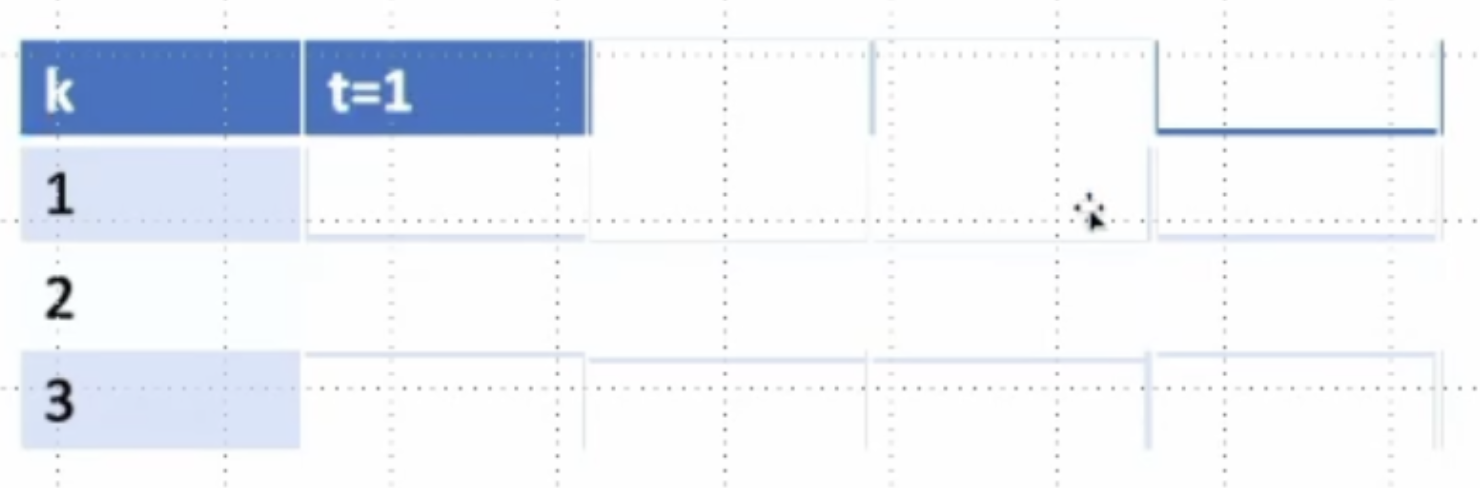
\includegraphics[width=0.75\linewidth]{images/multi_armed_bandit_example_1.png}

What would be the optimal strategy? Taking a glimpse at all possible values at each timestep, it should be clear that only getting partial feedback makes this problem extremely difficult

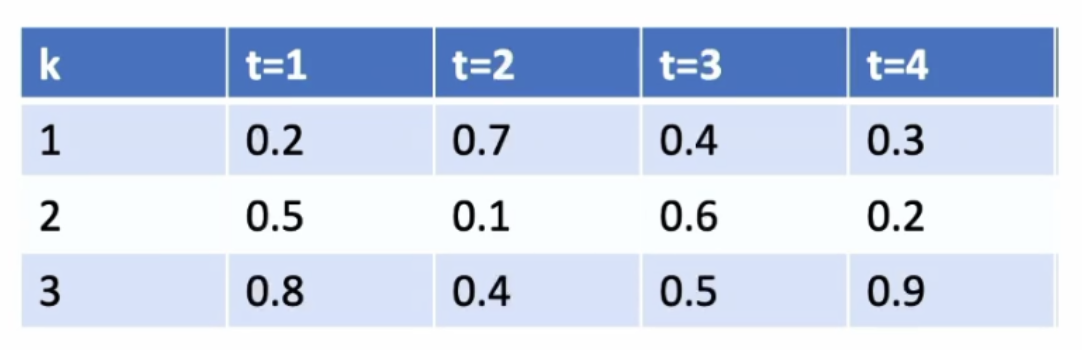
\includegraphics[width=0.75\linewidth]{images/multi_armed_bandit_example_2.png}

\textbf{Greedy Algorithm}: at each timestep, estimate a value for each action

\[ Q_t(a) = \frac {\text{sum of rewards when $a$ taken prior to $t$}} {\text{number of times $a$ taken prior to $t$}} = \frac {\sum_{i=1}^{t-1}r_i [[a_i = a]]} {\sum_{i=1}^{t-1}[[a_i = a]]} \]

and select the action with the maximum value

\[ a_t = \underset{a}{\text{argmax}} Q_t(a). \]

What are the properties of this solution? Here are some

\begin{itemize}
	\item Pro: Given the amount of information you have recieved, you minimize the amount of regret you would accumulate from the exploit aspect of the problem. In other words, you maximize the exploit aspect of the problem.

	\item Pro: If the variance of each arm is extremely small and the $\mu$ across arms are spread quite far, greedy will get the best total reward.

	\item Con: You don't explore efficiently enough, even to the point of certain outcomes being completely stuck with an unoptimal strategy (ex. an unoptimal strategy has been played observed too many times to have a $\mu$ that is lower than the observed $\mu$ of the optimal strategy because the optimal strategy was observed with low values a small number of times).

\end{itemize}

Obviously, this strategy is lacking in the exploration aspect of the problem. To solve this, we add a hyperparameter $\epsilon$ which represents the probability of exploring the existing actions rather than solely picking the ovserved optimal.\\

\textbf{$\epsilon$-Greedy Algorithm}: at time step $t$, estimate a value for each action

\[ Q_t(a) = \frac {\text{sum of rewards when $a$ taken prior to $t$}} {\text{number of times $a$ taken prior to $t$}} = \frac {\sum_{i=1}^{t-1}r_i [[a_i = a]]} {\sum_{i=1}^{t-1}[[a_i = a]]}. \]

With probability $1-\epsilon$, select the action with the maximum value (exploit)

\[ a_t = \underset{a}{\text{argmax}} Q_t(a). \]

With probability $\epsilon$, select an action uniformly at random from all the actions (i.e., each action selected with equal probability)\\

What are the properties of this solution? Here are some

\begin{itemize}
	\item Pro: No matter what, you continue to explore all actions no matter what, so you will never end up stuck in a non-optimal solution

	\item Con: You never stick with an optimal solution since you will always be switching (with a fixed probability) to non-optimal solutions during exploration

	\item Con: You consider actions during the exploration phase that are clearly out of the question for being the optimal arm. You should be able to probabilistically point out the arms that are in contention for being optimal and arms that are probabilistically impossible to be the optimal arm.

\end{itemize}

We can actually see the drawbacks of this strategy from the graphs below. It's clear that the more iterations you run this strategy for, this ``fixed" $\epsilon$-greedy algorithm will always begin to over explore options (unless $\epsilon = 0$). After 300 iterations, the total reward for $\epsilon = 0.1$ is the highest:

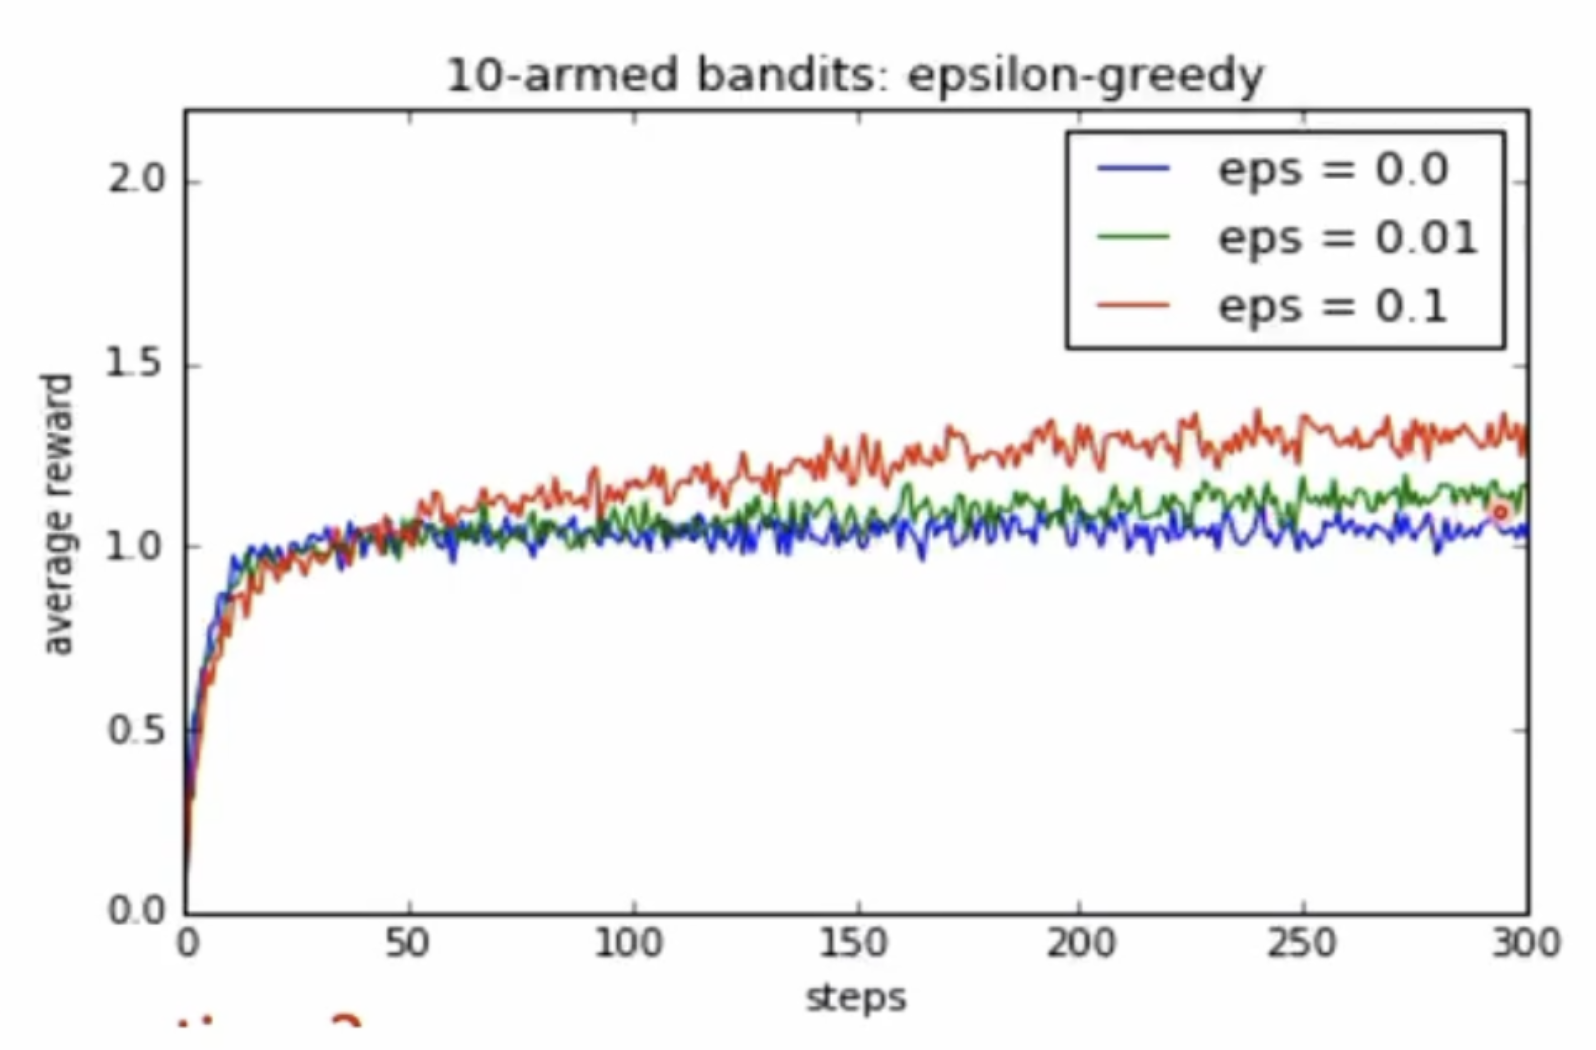
\includegraphics[width=0.75\linewidth]{images/multi_armed_bandit_example_3.png}

however, after 2000 iterations, the total reward for $\epsilon = 0.01$ outperforms $\epsilon = 0.1$

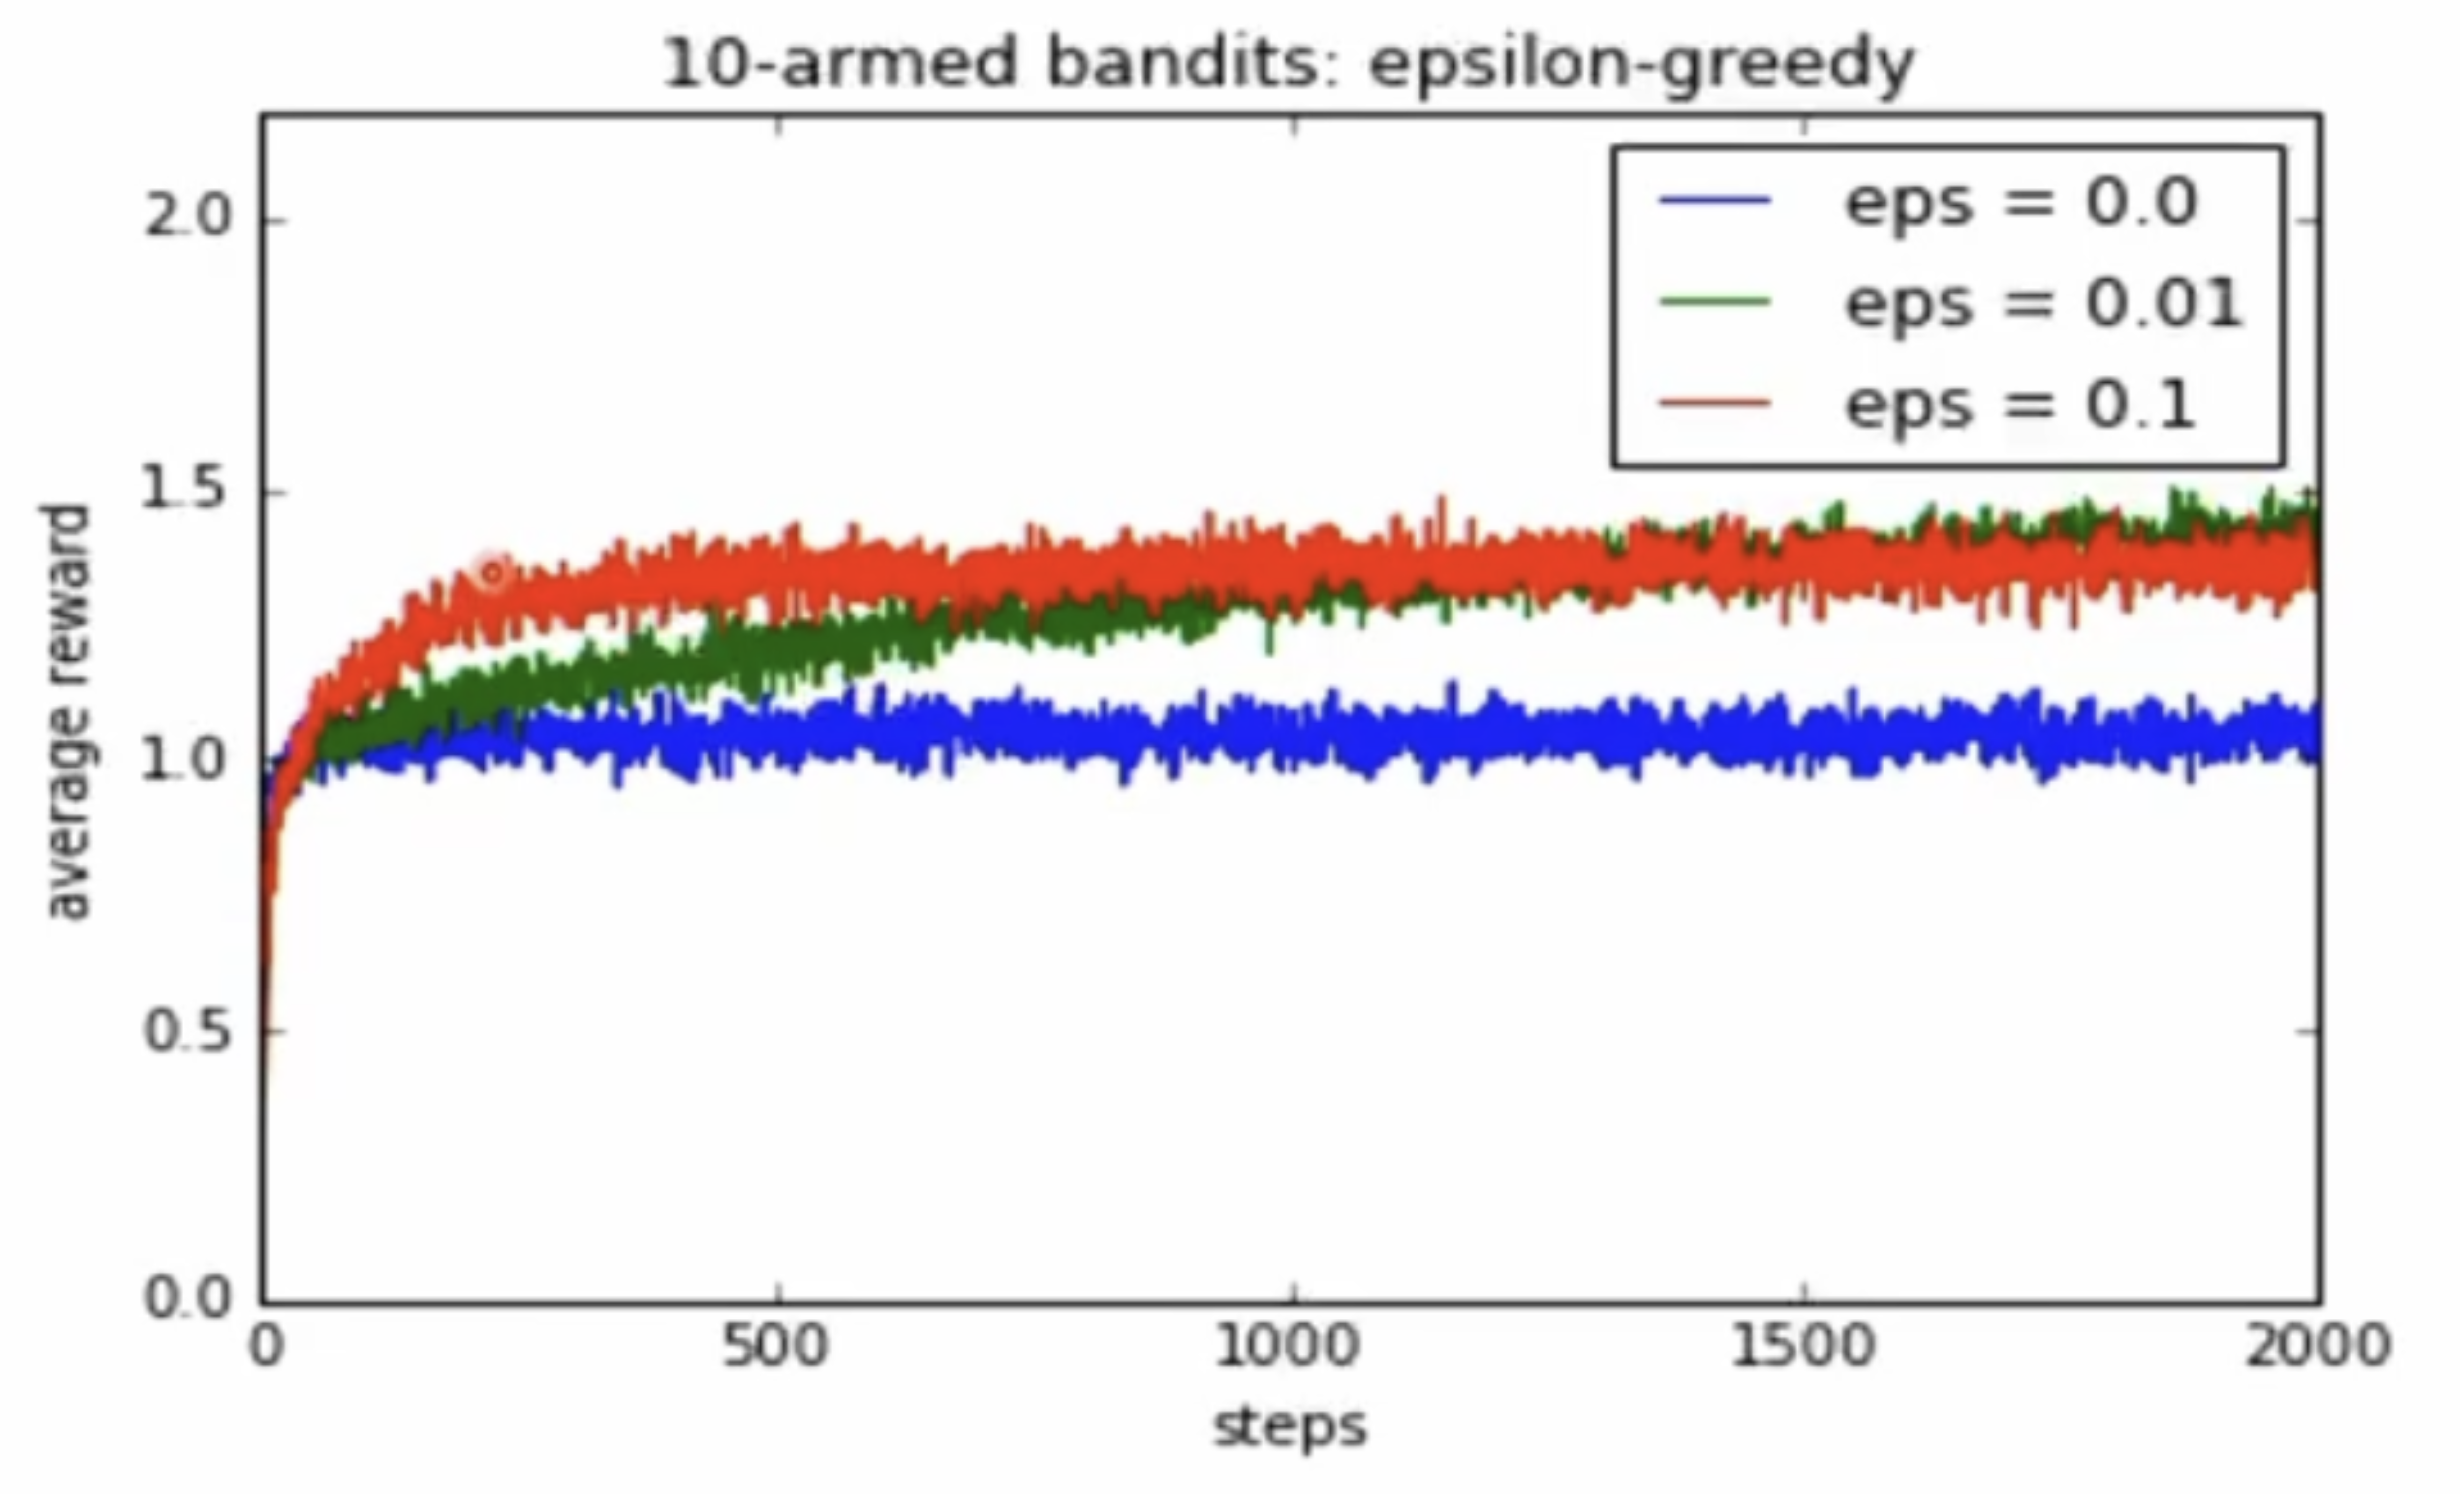
\includegraphics[width=0.75\linewidth]{images/multi_armed_bandit_example_4.png}

and you can imagine that for any $\epsilon > 0$, there exists $N$ where after $N$ iterations, a smaller $\epsilon$ starts to outperform that strategy.\\

One possible solution is decreasing the probability of exploration the more we explore. This is a nice balanced between exploring and exploiting that we wanted to find. However, this reintroduces a substantial probability of being stuck in an unoptimal arm. Instead, we will focus on the second con, which will conveniently solve our first con (honestly not sure about this. I'm pretty sure the optimal solution also decrease the probability of exploring as time goes on).\\

The main problem with this strategy is that during exploration, we are obliviously picking strategies without regards of existing information. What we should be doing instead is create confidence intervals on our arms to influence our action choice even in the exploration phase:\\

\textbf{Upper-Confidence-Bound Action Selection}: Select action maximizing upper-confidence-bound

\[ \underset{a}{\text{argmax}} \left[ Q_t(a) + c\sqrt{\frac {\ln t} {N_t(a)}} \right] \]

where $Q_t$ is the exploitation aspect, $c$ controls the degree of exploration, and the term after $c$ measures the degree of uncertainty for action $a$ through the following definition of function $N$:

\begin{itemize}
	\item Small $N_t(a) \rightarrow$ large confidence interval $\rightarrow Q_t(a)$ is more uncertain 
	\item Large $N_t(a) \rightarrow$ small confidence interval $\rightarrow Q_t(a)$ is less uncertain 
\end{itemize}

After examining the function, we see that this maintains the exploration phase and also introduces a confidence interval/degree of uncertainty where 

\begin{itemize}
	\item $t$ increases, but $N_t(a)$ does not
	\item as a result, the uncertainty estimate increases.
\end{itemize}

This means that the uncertainty of an action will grow unboundedly as it is continuously unchosen to be explored. So eventually every action will certainly (with a 100\% probability) be explored. For very unlikely events, we will still not rule out the possibility of it being the optimal (since there is always a non-zero chance of that action being the optimal) and thus we will still continue to explore all actions, but we will be picking it much much less than probable events.\\

GG

\newpage

\section{Final Exam Review}

\subsection{Parameter Counts}

\textbf{Fully Connected Neural Networks} with $n$ layers and $p_i$ non-bias neurons in layer $i$:

\[ \sum_{i = 2}^n p_i * (p_{i-1} + 1) \]

\textbf{CNN Convolutional Layer} with $n$ filters, each with dimensions $D \times H \times W$:

\[ n * (D*H*W + 1) \]

\textbf{CNN Batch/Layer Norm Layer}: 

\[ 2 \quad (\beta ~ \text{and} ~ \gamma) \]

\textbf{Gaussian} in $d$ dimenstions:

\[ 
	\begin{aligned}
		d + \frac {d(d-1)} 2 + d &\quad \text{mean + covariances + variances for general}\\
		d + 1 &\quad \text{mean + variance for spherical}
	\end{aligned}
\]

\textbf{GMM} with $k$ Guassians in $d$ dimenstions:

\[ 
	\begin{aligned}
		(k-1) + k(d + \frac {d(d-1)} 2 + d) &\quad \text{mixing coefficients + mean + covariances + variances for general}\\
		(k-1) + k(d + 1) &\quad \text{mixing coefficients + mean + variance for spherical}
	\end{aligned}
\]

\textbf{Bayesian Network} where each random variable $x_i$ can take on $r_i$ possible values for $i = 1, \dots, m$:

\[ \sum_{i = 1}^m (r_i - 1) \prod_{j \in pa_i} r_j \]

\newpage

\subsection{General Knowledge}:

\textbf{Ways to combat ``too small dataset" problem}:

\begin{itemize}
	\item Transfer Learning: Train a model on a similar source task with a much larger dataset to help with training on the smaller target task.
		\begin{enumerate}
			\item Pretrain a model with a source task $S'_m = \{ (\bar x^{(i)}, y^{(i)}) \}_{i=1}^m$.
			\item Freeze some number of layers $k$ and train the remaining $L-k$ layers on the target dataset. If $k = L-1$, this is called Linear Probing (only searching for the optimal final linear combination). If $k = 0$, this is called Fine-tuning (polishing the existing model to work on the target task).
		\end{enumerate}
	\item Data Augmentation: Augment individual datapoints in the dataset in a way so that the result is a different input (in the computers eyes) but should be classified exactly the same as before. Some common ways of augmentation are flipping, rotating or blocking parts of a image.
\end{itemize}

\textbf{Different forms of Attention}

\begin{itemize}
	\item Bidirectional self-attention: Default version of self-attention where each element in the sequence can attend to all other elements in the sequence.

		\[ \bar h_i = \sum_{j=1}^T softmax(s_{ij}) \bar v_j, \quad s_{ij} = \frac {\bar k_j \cdot \bar q_i} {\sqrt{d_k}} \]

		where 

		\[ 
			\begin{aligned}
				\text{``query"} & \bar q_i = W^Q \bar x_i & W^Q \in \R^{d_k \times d}\\
				\text{``key"} & \bar k_j = W^K \bar x_j & W^K \in \R^{d_k \times d}\\
				\text{``value"} & \bar v_j = W^V \bar x_j & W^V \in \R^{d_V \times d}\\
			\end{aligned}
		\]

	\item Causal-self attention (usually in the decoder): Allows each position in a sequence to attend to all positions up to and including that position. Math is the same as above except

		\[ 
			s_{ij} = \begin{cases}
				\frac {\bar k_j \cdot \bar q_i} {\sqrt{d_k}} & j \le i\\
				-\infty & \text{otherwise}
			\end{cases}
		\]
		
	\item Cross-attention: Queries come from previous output of the decoder layer and the keys and values come from the output of the encoder.\\

	\item Multi-head attention: multiple layers of attention blocks, each learning/capturing different patterns within a sequence.

		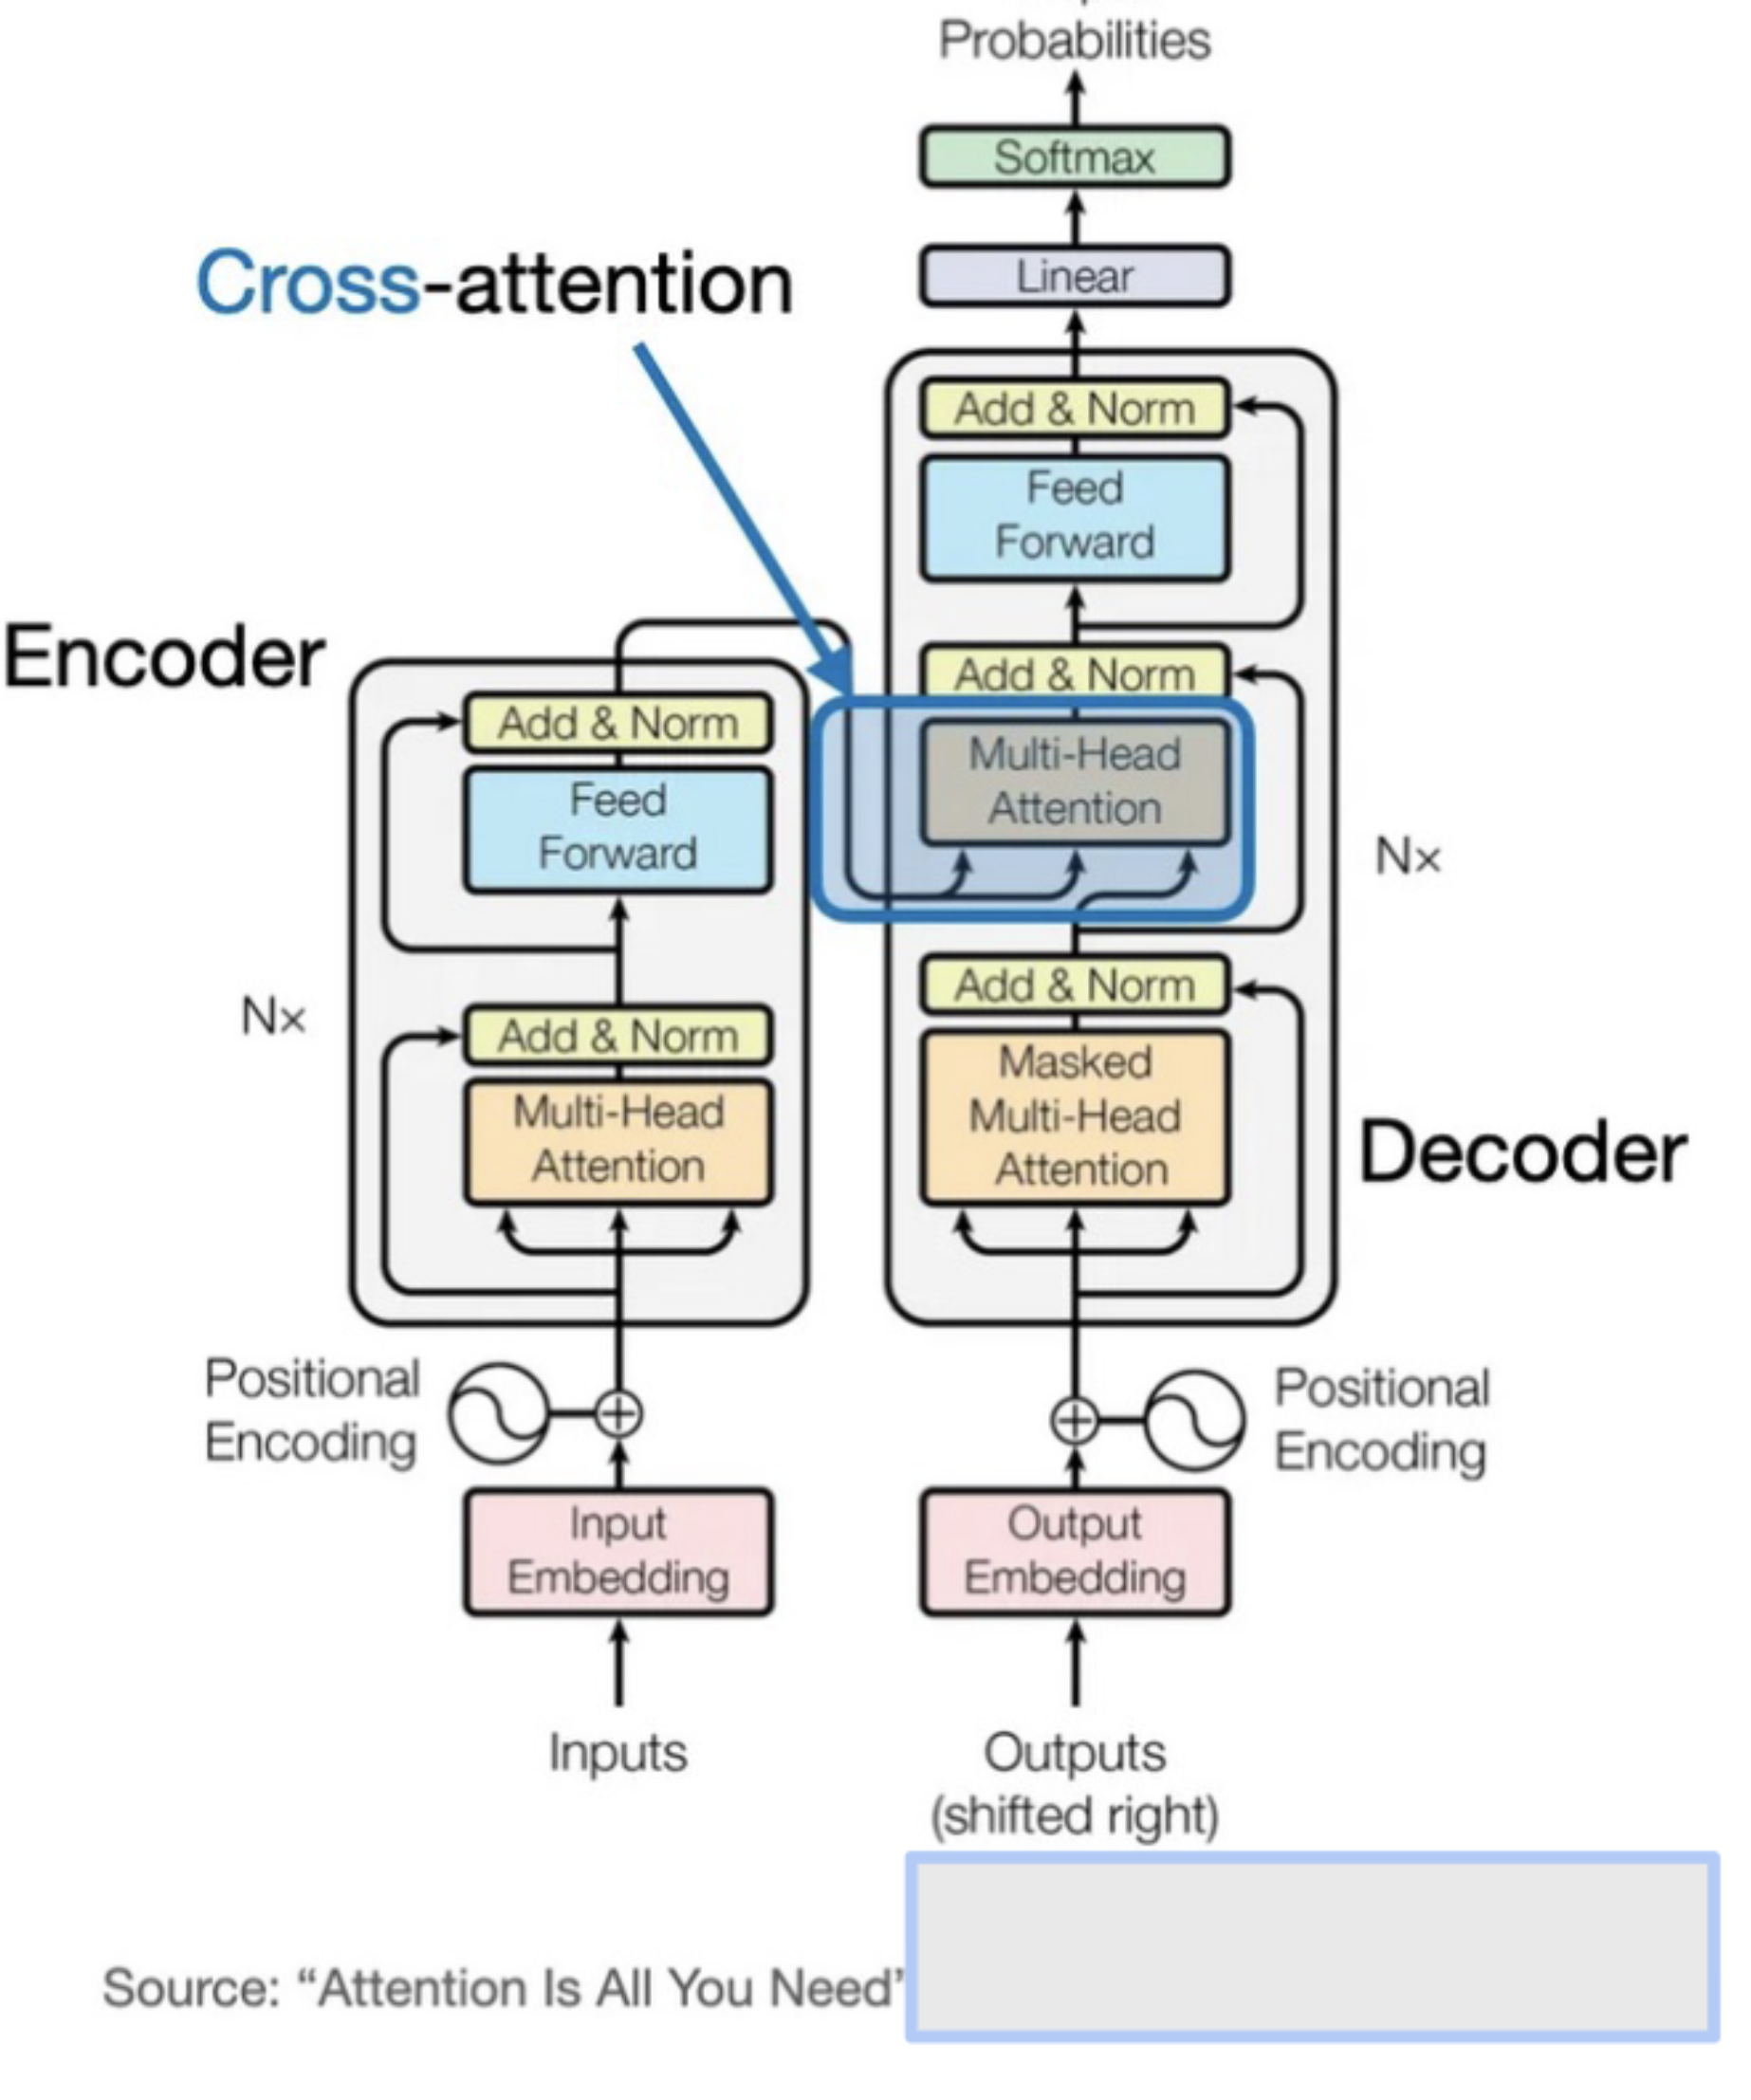
\includegraphics[width=0.25\linewidth]{images/types_of_transformers_example_1.png}
		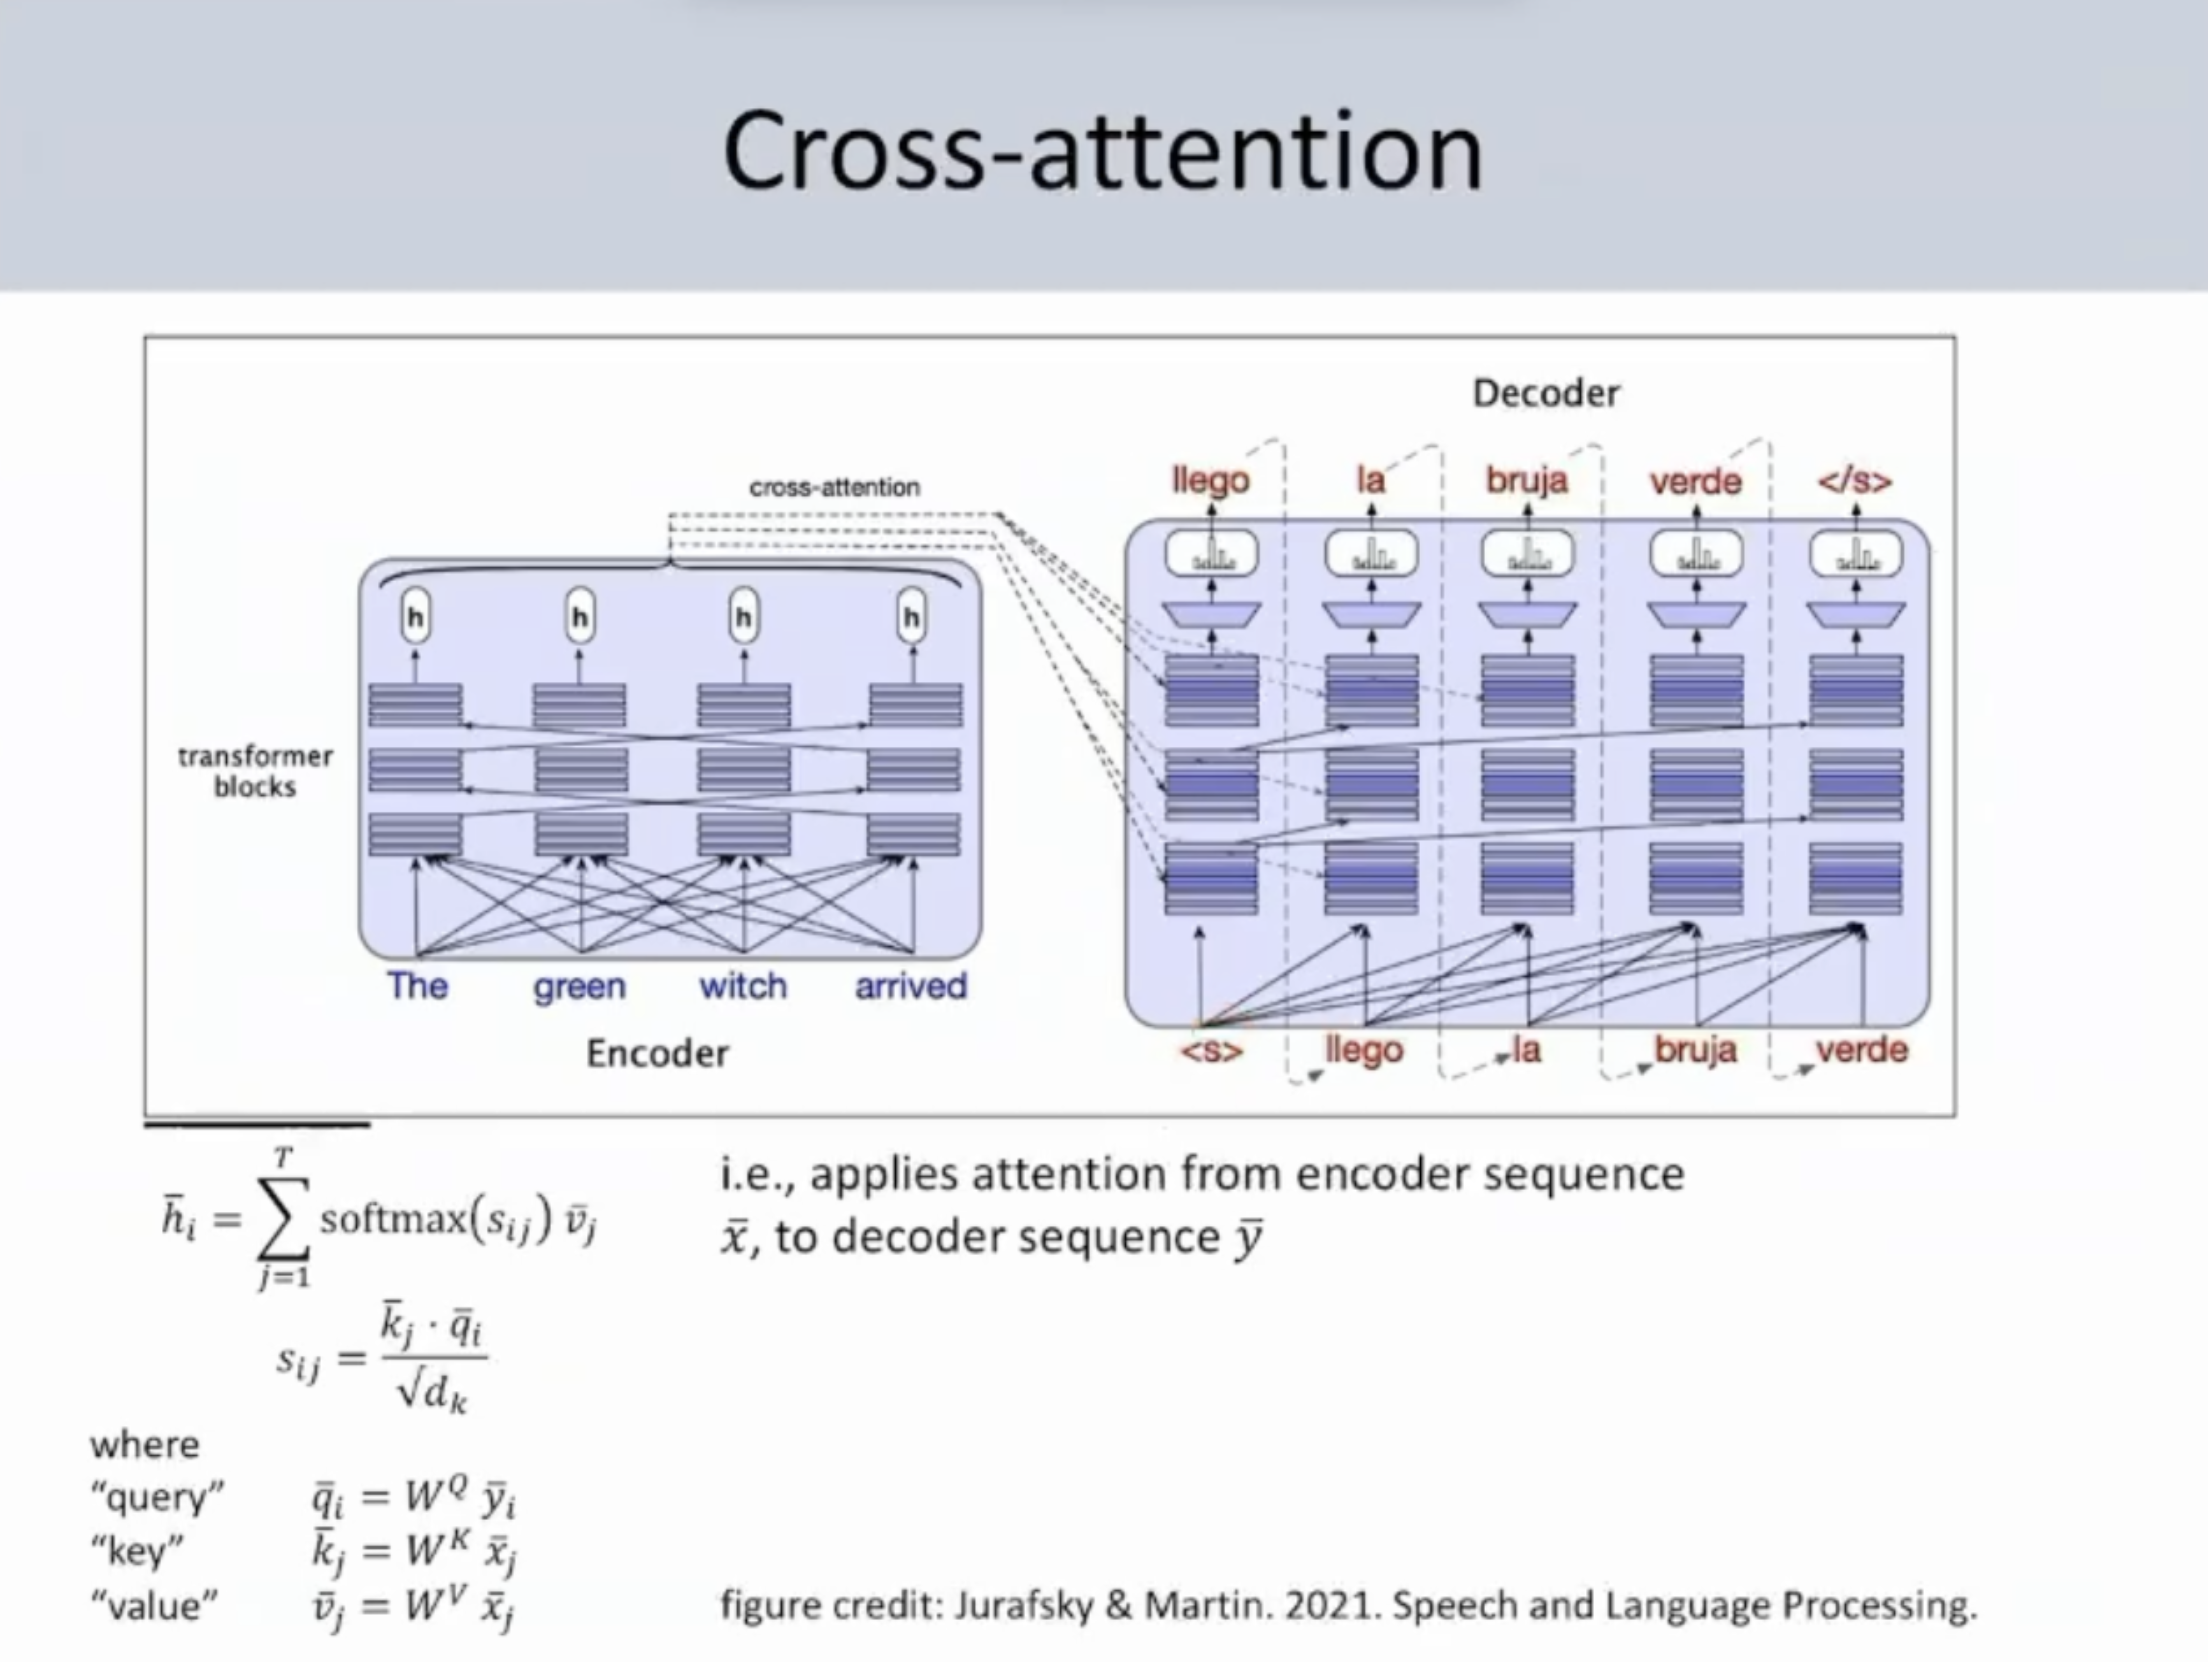
\includegraphics[width=0.25\linewidth]{images/types_of_transformers_example_2.png}
		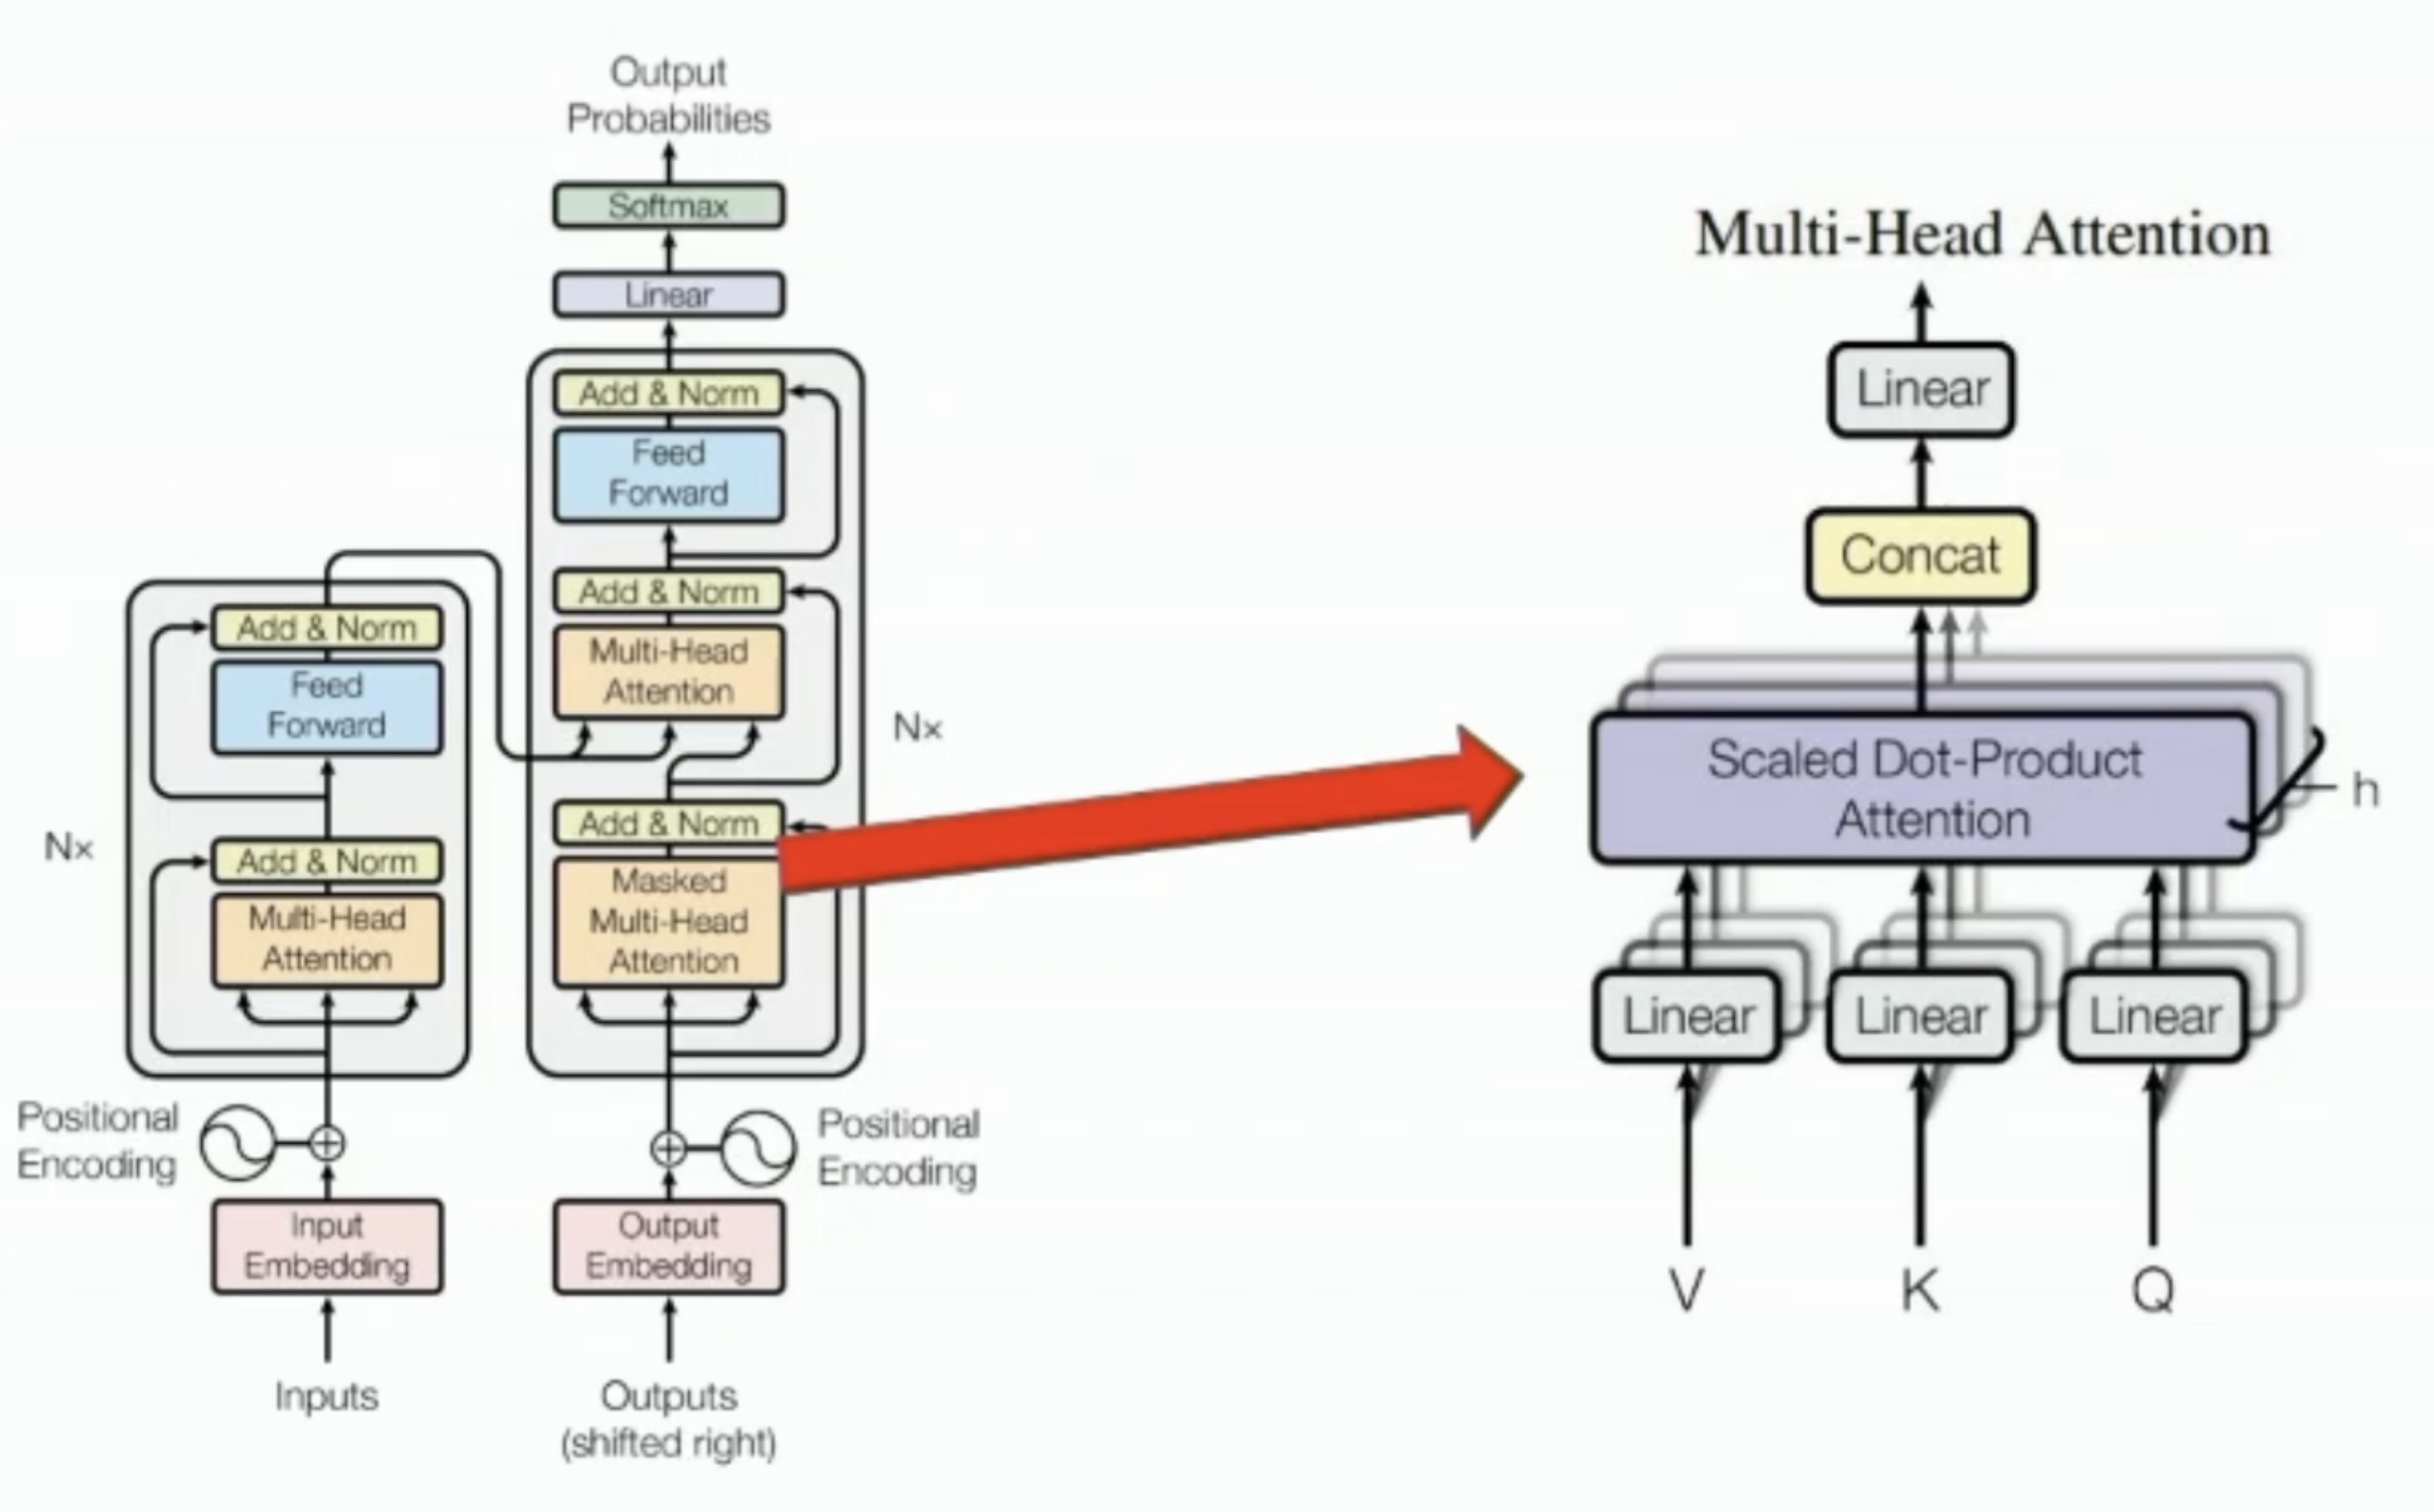
\includegraphics[width=0.25\linewidth]{images/types_of_transformers_example_3.png}

\end{itemize}

\end{document}

